\documentclass[lang=cn,newtx,10pt,scheme=chinese]{elegantbook}
\usepackage[utf8]{inputenc}
\usepackage[T1]{fontenc}
\usepackage{amsmath}
\usepackage{amsfonts}
\usepackage{amssymb}
\usepackage{stmaryrd}
\usepackage{hyperref}
\hypersetup{colorlinks=true, linkcolor=blue, filecolor=magenta, urlcolor=cyan,}
\urlstyle{same}
\usepackage{graphicx}
\usepackage[export]{adjustbox}
\usepackage{mdframed}
\usepackage{booktabs,array,multirow}
\usepackage{esint}
\usepackage{xeCJK}
\usepackage{adjustbox}
\newcommand{\HRule}{\begin{center}\rule{0.5\linewidth}{0.2mm}\end{center}}
\newcommand{\customfootnote}[1]{
	\let\thefootnote\relax\footnotetext{#1}
}

\title{高级中学课本 (试 用):微积分初步}
\subtitle{全一册(甲种本)}

\author{人民教育出版社数学室}
\institute{人民教育出版社}
\date{1985年 9 月}
\version{第 1 版}
\bioinfo{排版}{geezhu}

\extrainfo{人民教育出版社}

\setcounter{tocdepth}{3}

\logo{logo-blue.png}
\cover{cover.jpg}

% 本文档命令
\usepackage{array}
\newcommand{\ccr}[1]{\makecell{{\color{#1}\rule{1cm}{1cm}}}}

% 修改标题页的橙色带
\definecolor{customcolor}{RGB}{32,178,170}
\colorlet{coverlinecolor}{customcolor}
\usepackage{cprotect}

\addbibresource[location=local]{reference.bib} % 参考文献,不要删除

\begin{document}

\maketitle

\chapter*{说 明}
\markboth{说 明}{说 明}


一、本书供六年制中学高中三年级选用.

二、本书内容包括: 极限; 导数和微分; 导数的应用; 不定积分; 定积分及其应用. 学完这些内容, 约需 84 课时. 其中标有 “* ”号的内容, 供学生选学.

三、本书的习题共分三类: 练习

1. 练习 主要供课堂练习用. 编辑

2. 习题 主要供课内外作业 \(\nabla = 0\) 时

3. 复习参考题 在每章后配包组题主要供复习本章知识时使用; B 组题略带综合性、灵活性, 仅供学有余力的学生参考使用.

为了使教学更有针对性和灵活性, 本书配备的练习、习题和复习参考题 \(A\) 组数量较多,便于教学时根据实际情况选用.

四、本书在编写过程中, 曾参考了中小学通用教材数学编写组编写的全日制十年制学校高中课本(试用本)《数学》第四册的有关章节, 大部分内容是以原来章节为基础编写的.

五、本书由人民教育出版社数学室编写. 参加编写工作的有方明一、刘远图、曾宪源、于琛等。全书由于琛校订。

\frontmatter

\tableofcontents

\mainmatter

\chapter{极 限}

\begin{quotation}
	\textbf{\textcolor{red}{本模板自 2023 年 1 月 1 日开始,不再维护,不建议使用本系列模板!为了保证之前版本的用户仍然能查到说明文档,本说明文档仍然保留过去的信息。}}
\end{quotation}

Elegant\LaTeX{} 项目组致力于打造一系列美观、优雅、简便的模板方便用户使用。目前由 \href{https://github.com/ElegantLaTeX/ElegantNote}{ElegantNote},\href{https://github.com/ElegantLaTeX/ElegantBook}{ElegantBook},\href{https://github.com/ElegantLaTeX/ElegantPaper}{ElegantPaper} 组成,分别用于排版笔记,书籍和工作论文。大版本改动较大,请关注版本信息,在未开始使用模板前,建议直接选择最新正式版本!


本文将介绍本模板的一些设置内容以及基本使用方法。如果您有其他问题,建议或者意见,欢迎在 GitHub 上给我们提交 \href{https://github.com/ElegantLaTeX/ElegantBook/issues}{issues} 或者邮件联系我们。我们的联系方式如下,建议加入用户 QQ 群提问,这样能更快获得准确的反馈,加群时请备注 \LaTeX{} 或者 Elegant\LaTeX{} 相关内容。
\begin{itemize}
	\item 官网:\href{https://elegantlatex.org/}{https://elegantlatex.org/}
	\item GitHub 地址:\href{https://github.com/ElegantLaTeX/}{https://github.com/ElegantLaTeX/}
	\item CTAN 地址:\href{https://ctan.org/pkg/elegantbook}{https://ctan.org/pkg/elegantbook}
	\item 下载地址:\href{https://github.com/ElegantLaTeX/ElegantBook/releases}{正式发行版},\href{https://github.com/ElegantLaTeX/ElegantBook/archive/master.zip}{最新版}
	\item Bilibili:\href{https://space.bilibili.com/516479629}{ElegantLaTeX}
	\item 用户 QQ 群:692108391
\end{itemize}


\section{数列的极限}

我们来考察下面两个数列:

\[
1,\frac{1}{2},\frac{1}{3},\cdots \cdots ,\frac{1}{n},\cdots \tag{1}
\]

\[
\frac{1}{2},\frac{3}{4},\frac{7}{8},\cdots \cdots ,1 - \frac{1}{{2}^{n}},\cdots \text{.} \tag{2}
\]

为了直观起见, 我们把这两个数列中的前几项分别在数轴上表示出来(图 1-1):

\begin{center}
	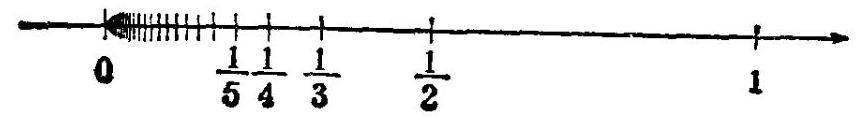
\includegraphics[width=0.5\textwidth]{images/01912c18-5c3f-733d-b775-749ba9897a9d_4_159408.jpg}

\end{center}

\begin{center}
	(1)
\end{center}


\begin{center}
	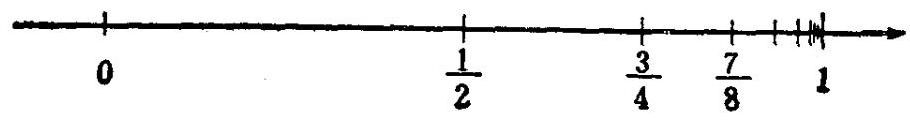
\includegraphics[width=0.5\textwidth]{images/01912c18-5c3f-733d-b775-749ba9897a9d_4_459236.jpg}
\end{center}

图 1-1

容易看出,当项数 \(n\) 无限增大时,数列 (1) 中的项无限趋近于 0 , 数列 (2) 中的项无限趋近于 1 .

事实上, 在数列 (1) 中, 各项与 0 的差的绝对值如下页的表所示.

我们看到,无论预先指定多么小的一个正数 \(\varepsilon\) ,总能在

\begin{center}
	\adjustbox{max width=\textwidth}{
		\begin{tabular}{|c|c|c|}
			\hline
			项 号 & 项 & 这一项与 0 的差的绝对值 \\
			\hline
			1 & 1 & \(\left| {0 - 1}\right| = 1\) \\
			\hline
			2 & \(\frac{1}{2}\) & \(\left| {0 - \frac{1}{2}}\right| = \frac{1}{2}\) \\
			\hline
			3 & \(\frac{1}{3}\) & \(\left| {0 - \frac{1}{3}}\right| = \frac{1}{3}\) \\
			\hline
			4 & \(\frac{1}{4}\) & \(\left| {0 - \frac{1}{4}}\right| = \frac{1}{4}\) \\
			\hline
			5 & \(\frac{1}{5}\) & \(\left| {0 - \frac{1}{5}}\right| = \frac{1}{5}\) \\
			\hline
			6 & \(\frac{1}{6}\) & \(\left| {0 - \frac{1}{6}}\right| = \frac{1}{6}\) \\
			\hline
			7 & \(\frac{1}{7}\) & \(\left| {0 - \frac{1}{7}}\right| = \frac{1}{7}\) \\
			\hline
			... & \(\cdots\) & \(\cdots\) \\
			\hline
		\end{tabular}
	}
\end{center}

数列 (1) 中找到这样一项, 使得这一项后面的所有项与 0 的差的绝对值都小于 \(\varepsilon\) . 例如,如果取 \(\varepsilon = \frac{1}{5}\) ,那么数列 (1) 中第 5 项后面所有的项与 0 的差的绝对值都小于 \(\varepsilon\) . 如果取 \(\varepsilon = \frac{1}{100}\) , 那么数列 (1) 中第 100 项后面所有的项与 0 的差的绝对值都小于 \(\varepsilon\) . 在这种情况下,我们就说数列 (1) 的极限是 0 .

同样, 对于数列 (2), 我们也可以列成下页的表.

可以看出,如果取 \(\varepsilon = {0.1}\) ,那么数列 (2) 中第 3 项后面所有的项与 1 的差的绝对值都小于 \(\varepsilon\) ; 如果取 \(\varepsilon = {0.01}\) ,那么第 6 项后面所有的项与 1 的差的绝对值都小于 \(\varepsilon\) . 就是说,无论预先指定多么小的一个正数 \(\varepsilon\) ,总能在数列(2)中找到这样一

\begin{center}
	\adjustbox{max width=\textwidth}{
		\begin{tabular}{|c|c|c|}
			\hline
			项 号 & 项 & 这一项与 1 的差的绝对值 \\
			\hline
			1 & \(\frac{1}{2}\) & \(\left| {\frac{1}{2} - 1}\right| = \frac{1}{2} = {0.5}\) \\
			\hline
			2 & \(\frac{3}{4}\) & \(\left| {\frac{3}{4} - 1}\right| = \frac{1}{4} = {0.25}\) \\
			\hline
			3 & \(\frac{7}{8}\) & \(\left| {\frac{7}{8} - 1}\right| = \frac{1}{8} = {0.125}\) \\
			\hline
			4 & \(\frac{15}{16}\) & \(\left| {\frac{15}{16} - 1}\right| = \frac{1}{16} = {0.0625}\) \\
			\hline
			5 & \(\frac{31}{32}\) & \(\left| {\frac{31}{32} - 1}\right| = \frac{1}{32} = {0.03125}\) \\
			\hline
			6 & \(\frac{63}{64}\) & \(\left| {\frac{63}{64} - 1}\right| = \frac{1}{64} = {0.015625}\) \\
			\hline
			7 & \(\frac{127}{128}\) & \(\left| {\frac{127}{128} - 1}\right| = \frac{1}{128} = {0.0078125}\) \\
			\hline
			\(\cdots\) & \(\cdots\) & \(\cdots\) \\
			\hline
		\end{tabular}
	}
\end{center}

项,使得这一项后面的所有项与 1 的差的绝对值都小于 \(\varepsilon\) . 这时, 我们说数列 (2) 的极限是 1 .

一般地,对于一个无穷数列 \(\left\{ {a}_{n}\right\}\) ,如果存在一个常数 \(A\) , 无论预先指定多么小的正数 \(\varepsilon\) ,都能在数列中找到一项 \({a}_{N}\) ,使得这一项后面所有的项与 \(A\) 的差的绝对值都小于 \(\varepsilon\) (即当 \(n >\) \(N\) 时, \(\left| {{a}_{n} - A}\right| < \varepsilon\) 恒成立),就把常数 \(A\) 叫做数列 \(\left\{ {a}_{n}\right\}\) 的极限, 记作

\[
\mathop{\lim }\limits_{{n \rightarrow \infty }}{a}_{n} = A\text{. O }
\]

这个式子读作 “当 \(n\) 趋向于无穷大时, \({a}_{n}\) 的极限等于 \({A}^{n}\) . “->” 表示 “趋向于”, “ \(\infty\) ” 表示 “无穷大”, “ \(n \rightarrow \infty\) ” 表示 “ \(n\) 趋向于无穷大”,也就是 \(n\) 无限增大的意思.

\customfootnote{
	
	O lim 是拉丁文 limis (极限) 一词的前三个字母, 一般按英文 limit (极限) 一词读音. \(\mathop{\lim }\limits_{{n \rightarrow \infty }}{a}_{n} = A\) 也可读作 “limit \({a}_{n}\) 当 \(n\) 趋于无穷大时等于 \({A}^{n}\) .
	
}

\(\mathop{\lim }\limits_{{n \rightarrow \infty }}{a}_{n} = A\) 有时也可记作

\[
\text{当}n \rightarrow \infty \text{时,}{a}_{n} \rightarrow A\text{.}
\]

从数列极限的定义可以看出,数列 \(\left\{ {a}_{n}\right\}\) 以 \(A\) 为极限,是指当 \(n\) 无限增大时,数列 \(\left\{ {a}_{n}\right\}\) 中的项 \({a}_{n}\) 无限趋近于常数 \(A\) .

例 1 已知数列

\[
1, - \frac{1}{2},\frac{1}{3}, - \frac{1}{4},\cdots ,{\left( -1\right) }^{n + 1}\frac{1}{n},\cdots \text{.}
\]

(1) 写出这个数列的各项与 0 的差的绝对值.

(2)第几项后面所有的项与 0 的差的绝对值都小于 0.1 ? 都小于 0.001 ? 都小于 0.0003 ?

(3)第几项后面所有的项与 0 的差的绝对值都小于任何预先指定的正数 \(\varepsilon\) ?

(4) 0 是不是这个数列的极限?

解: 这个数列的项在数轴上的表示如图 1-2:

\begin{center}
	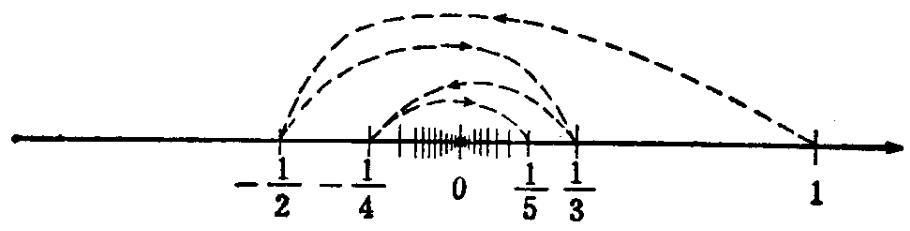
\includegraphics[max width=0.9\textwidth]{images/01912c18-5c3f-733d-b775-749ba9897a9d_7_608223.jpg}
\end{center}

图 1-2

(1)这个数列的各项与 0 的差的绝对值依次是

\[
1,\frac{1}{2},\frac{1}{3},\cdots ,\frac{1}{n},\cdots
\]

(2)要使 \(\frac{1}{n} < {0.1}\) ,只要 \(n > {10}\) 就行了. 这就是说,第 10 项后面所有的项与 0 的差的绝对值都小于 0.1 .

要使 \(\frac{1}{n} < {0.001}\) ,只要 \(n > {1000}\) 就行了. 这就是说,第 1000 项后面所有的项与 0 的差的绝对值都小于 0.001 .

要使 \(\frac{1}{n} < {0.0003}\) ,只要 \(n > {3333}\frac{1}{3}\) 就行了. 这就是说,第 3333 项后面所有的项与 0 的差的绝对值都小于 0.0003 .

(3)要使 \(\frac{1}{n} < \varepsilon\) ,只要 \(n > \frac{1}{\varepsilon }\) 就行了,因为所求的项数必须是正整数,因此设 \(\frac{1}{e}\) 的整数部分是 \(N\) ,那么第 \(N\) 项后面所有的项与 0 的差的绝对值都小于 \(\varepsilon\) .

(4)从(3)可以知道, 0 是这个数列的极限, 记作:

\[
\mathop{\lim }\limits_{{n \rightarrow \infty }}{\left( -1\right) }^{n + 1}\frac{1}{n} = 0
\]

例 2 已知数列

\[
\frac{1}{2},\frac{2}{3},\frac{3}{4},\cdots ,\frac{n}{n + 1},\cdots
\]

(1) 计算 \(\left| {{a}_{n} - 1}\right|\) .

(2)第几项后面所有的项与 1 的差的绝对值都小于 \(\frac{1}{100}\) ?

(3)第几项后面所有的项与 1 的差都小于任意指定的正数 \({\varepsilon }_{2}\)

(4) 1 是不是这个数列的极限?

解: (1) \(\left| {{a}_{n} - 1}\right| = \left| {\frac{n}{n + 1} - 1}\right| = \left| \frac{-1}{n + 1}\right| = \frac{1}{n + 1}\) .

(2)要使 \(\frac{1}{n + 1} < \frac{1}{100}\) ,就是要使 \(n + 1 > {100}\) ,即 \(n > {99}\) ,这就是说,第 99 项后面所有的项与 1 的差的绝对值都小于 \(\frac{1}{100}\) .

(3)要使 \(\frac{1}{n + 1} < \varepsilon\) ,就是要使 \(n + 1 > \frac{1}{\varepsilon }\) ,即 \(n > \frac{1}{\varepsilon } - 1\) ,设 \(\frac{1}{\varepsilon } - 1\) 的整数部分是 \(N\) ,那么第 \(N\) 项后面所有的项与 1 的差的绝对值都小于正数 \(\varepsilon\) .

(4) 从 (3) 可以知道, 这个数列的极限是 1 , 记作:

\[
\mathop{\lim }\limits_{{n \rightarrow \infty }}\frac{n}{n + 1} = 1
\]

例 3 已知数列

\[
\frac{1}{2},\frac{1}{4},\frac{1}{8},\cdots ,\frac{1}{{2}^{n}}\cdots
\]

(1) 计算 \(\left| {{a}_{n} - 0}\right|\) .

(2)第几项后面所有的项与 0 的差的绝对值小于正数 \(\varepsilon\) ?

(3) 0 是不是这个数列的极限?

解: (1) \(\left| {{a}_{n} - 0}\right| = \left| {\frac{1}{{2}^{n}} - 0}\right| = \frac{1}{{2}^{n}}\) .

(2)要使 \(\frac{1}{{2}^{n}} < \varepsilon\) ,就是要使 \(n > \frac{\ln \frac{1}{\varepsilon }}{\ln 2}\) . 设 \(\frac{\ln \frac{1}{\varepsilon }}{\ln 2}\) 的整数部分是 \(N\) ,那么第 \(N\) 项后面所有的项与 0 的差的绝对值都小于正数 \(\varepsilon\) .

(3)从 \(\left( 2\right)\) 可以知道,这个数列的极限是 0 ,记作

\[
\mathop{\lim }\limits_{{n \rightarrow \infty }}\frac{1}{{2}^{n}} = 0
\]

例 4 求常数数列 \(- 7, - 7, - 7,\cdots\) 的极限.

解: 这个数列的各项与 -7 的差的绝对值都等于 0 , 所以从第 1 项起,这个绝对值就能够小于任意指定的正数 \(\varepsilon\) ,因此这个数列的极限是 -7 .

一般地, 任何一个常数数列的极限都是这个常数本身, 即

\[
\mathop{\lim }\limits_{{n \rightarrow \infty }}C = C\text{ ( }C\text{ 是常数). }
\]

应该指出, 并不是每一个无穷数列都有极限. 例如, 数列

\[
1,2,3,\cdots ,n,\cdots
\]

就没有极限.

数列

\[
- 1,1, - 1,1,\cdots ,{\left( -1\right) }^{n},\cdots
\]

也没有极限.

\begin{problemset}[练习]
	\item 已知数列
	
	\[
	\frac{1}{{1}^{2}},\frac{1}{{2}^{2}},\frac{1}{{3}^{2}},\frac{1}{{4}^{2}},\cdots ,\frac{1}{{n}^{2}},\cdots
	\]
	
	(1)把这个数列的前 5 项在数轴上表示出来。
	
	(2)写出这个数列的各项与 0 的差的绝对值。
	
	(3)第几项后面的所有项与 0 的差的绝对值都小于 0.1 ? 都小于 0.01 ? 都小于 0.00011 都小于任何预先指定的正数 \(\varepsilon\) ?
	
	(4)是不是这个无穷数列的极限?
	
	\item 已知数列 \(4 - \frac{1}{10},4 - \frac{1}{20},4 - \frac{1}{30},\cdots ,4 - \frac{1}{10n},\cdots\) .
	
	(1) 计算 \(\left| {{a}_{n} - 4}\right|\) .
	
	(2) 第几项后面的所有项与 4 的差的绝对值都小于 0.01 ? 都小于任意指定的正数 \(\varepsilon\) ?
	
	(3) 确定这个数列的极限。
\end{problemset}



\section{数列极限的四则运算}
前面我们看到, 一些简单的数列可以从变化趋势找出它们的极限. 例如,

\[
\mathop{\lim }\limits_{{n \rightarrow \infty }}\frac{1}{n} = 0,\;\mathop{\lim }\limits_{{n \rightarrow \infty }}\frac{1}{{2}^{n}} = 0,\;\mathop{\lim }\limits_{{n \rightarrow \infty }}C = C.
\]

如果求极限的数列比较复杂, 就要分析已知数列是由哪些简单的数列经过怎样的运算结合而成的, 这样就能把复杂的数列的极限的计算问题转化为简单的数列的极限的计算问题. 因此, 下面引入数列极限的四则运算法则 (证明从略):

\[
\text{如果}\mathop{\lim }\limits_{{n \rightarrow \infty }}{a}_{n} = A,\mathop{\lim }\limits_{{n \rightarrow \infty }}{b}_{n} = B\text{,那么,}
\]

\[
\mathop{\lim }\limits_{{n \rightarrow \infty }}\left( {{a}_{n} \pm {b}_{n}}\right) = A \pm B
\]

\[
\mathop{\lim }\limits_{{n \rightarrow \infty }}\left( {{a}_{n} \cdot {b}_{n}}\right) = A \cdot B
\]

\[
\mathop{\lim }\limits_{{n \rightarrow \infty }}\frac{{a}_{n}}{{b}_{n}} = \frac{A}{B}\left( {B \neq 0}\right) .
\]

特别地,如果 \(C\) 是常数,那么,

\[
\mathop{\lim }\limits_{{n \rightarrow \infty }}\left( {C \cdot {a}_{n}}\right) = \mathop{\lim }\limits_{{n \rightarrow \infty }}C \cdot \mathop{\lim }\limits_{{n \rightarrow \infty }}{a}_{n} = {CA}.
\]

上面的数列极限的四则运算法则表明: 如果两个数列都有极限, 那么, 这两个数列的各对应项的和、差、积、商组成的数列的极限, 分别等于这两个数列的极限的和、差、积、商 (各项作为除数的数列的极限不能为零).

例如, 数列

\[
\frac{1}{2},\frac{2}{3},\frac{3}{4},\cdots ,\frac{n}{n + 1},\cdots
\]

与

\[
2,2,2,\cdots ,2,\cdots
\]

的极限分别是 1 与 2 , 那么根据上面的运算法则, 这两个数列的各对应项的和组成的数列

\[
2 + \frac{1}{2},2 + \frac{2}{3},2 + \frac{3}{4},\cdots ,2 + \frac{n}{n + 1},\cdots
\]

的极限是 3 .

例 1 已知 \(\mathop{\lim }\limits_{{n \rightarrow \infty }}{a}_{n} = 5,\mathop{\lim }\limits_{{n \rightarrow \infty }}{b}_{n} = 3\) ,求 \(\mathop{\lim }\limits_{{n \rightarrow \infty }}\left( {3{a}_{n} - 4{b}_{n}}\right)\) .

解: \(\mathop{\lim }\limits_{{n \rightarrow \infty }}\left( {3{a}_{n} - 4{b}_{n}}\right) = \mathop{\lim }\limits_{{n \rightarrow \infty }}3{a}_{n} - \mathop{\lim }\limits_{{n \rightarrow \infty }}4{b}_{n}\)

\[
= 3\mathop{\lim }\limits_{{n \rightarrow \infty }}{a}_{n} - 4\mathop{\lim }\limits_{{n \rightarrow \infty }}{b}_{n} = 3 \times 5 - 4 \times 3 = 3\text{.}
\]

例 2 求:

(1) \(\mathop{\lim }\limits_{{n \rightarrow \infty }}\left( {5 + \frac{1}{n}}\right)\) (2) \(\mathop{\lim }\limits_{{n \rightarrow \infty }}\frac{{3n} - 2}{n}\)

(3) \(\mathop{\lim }\limits_{{n \rightarrow \infty }}\frac{{2n} + 1}{{3n} + 2}\) (4) \(\mathop{\lim }\limits_{{n \rightarrow \infty }}\frac{3{n}^{2} - {2n} + 8}{4 - {n}^{2}}\) .

解: (1) \(\mathop{\lim }\limits_{{n \rightarrow \infty }}\left( {5 + \frac{1}{n}}\right) = \mathop{\lim }\limits_{{n \rightarrow \infty }}5 + \mathop{\lim }\limits_{{n \rightarrow \infty }}\frac{1}{n}\)

\[
= 5 + 0 = 5\text{. }
\]

(2) \(\mathop{\lim }\limits_{{n \rightarrow \infty }}\frac{{3n} - 2}{n} = \mathop{\lim }\limits_{{n \rightarrow \infty }}\left( {\frac{3n}{n} - \frac{2}{n}}\right)\)

\[
= \mathop{\lim }\limits_{{n \rightarrow \infty }}3 - \mathop{\lim }\limits_{{n \rightarrow \infty }}\left( {2 \cdot \frac{1}{n}}\right) = 3 - 2\mathop{\lim }\limits_{{n \rightarrow \infty }}\frac{1}{n}
\]

\[
= 3 - 2 \times 0 = 3\text{. }
\]

(3)当 \(n\) 无限增大时,分式 \(\frac{{2n} + 1}{{3n} + 2}\) 中的分子、分母同时无限增大, 上面的极限运算法则不能直接运用. 为此, 我们将分式中的分子、分母同时除以 \(n\) 后求它的极限,得

\[
\mathop{\lim }\limits_{{n \rightarrow \infty }}\frac{{2n} + 1}{{3n} + 2} = \mathop{\lim }\limits_{{n \rightarrow \infty }}\frac{2 + \frac{1}{n}}{3 + \frac{2}{n}}
\]

\[
= \frac{\mathop{\lim }\limits_{{n \rightarrow \infty }}\left( {2 + \frac{1}{n}}\right) }{\mathop{\lim }\limits_{{n \rightarrow \infty }}\left( {3 + \frac{2}{n}}\right) } = \frac{\mathop{\lim }\limits_{{n \rightarrow \infty }}2 + \mathop{\lim }\limits_{{n \rightarrow \infty }}\frac{1}{n}}{\mathop{\lim }\limits_{{n \rightarrow \infty }}3 + \mathop{\lim }\limits_{{n \rightarrow \infty }}\frac{2}{n}}
\]

\[
= \frac{2 + 0}{3 + 0} = \frac{2}{3}
\]

(4) \(\mathop{\lim }\limits_{{n \rightarrow \infty }}\frac{3{n}^{2} - {2n} + 8}{4 - {n}^{2}} = \mathop{\lim }\limits_{{n \rightarrow \infty }}\frac{3 - \frac{2}{n} + \frac{8}{{n}^{2}}}{\frac{4}{{n}^{2}} - 1}\)

\[
= \frac{\mathop{\lim }\limits_{{n \rightarrow \infty }}\left( {3 - \frac{2}{n} + \frac{8}{{n}^{2}}}\right) }{\mathop{\lim }\limits_{{n \rightarrow \infty }}\left( {\frac{4}{{n}^{2}} - 1}\right) } = \frac{\mathop{\lim }\limits_{{n \rightarrow \infty }}3 - \mathop{\lim }\limits_{{n \rightarrow \infty }}\frac{2}{n} + \mathop{\lim }\limits_{{n \rightarrow \infty }}\frac{8}{{n}^{2}}}{\mathop{\lim }\limits_{{n \rightarrow \infty }}\frac{4}{{n}^{2}} - \mathop{\lim }\limits_{{n \rightarrow \infty }}1}.
\]

\[
= \frac{3 - 0 + 0}{0 - 1} = - 3\text{. }
\]

例 3 已知等比数列

\[
\frac{1}{2},\frac{1}{4},\frac{1}{8},\cdots ,\frac{1}{{2}^{n}},\cdots
\]

求这个数列前 \(n\) 项的和当 \(n \rightarrow \infty\) 时的极限.

解: 这个等比数列的公比是

\[
q = \frac{\frac{1}{4}}{\frac{1}{2}} = \frac{1}{2}.
\]

根据等比数列前 \(n\) 项和的公式,得

\[
{S}_{n} = \frac{{a}_{1}\left( {1 - {q}^{n}}\right) }{1 - q} = \frac{\frac{1}{2}\left\lbrack {1 - {\left( \frac{1}{2}\right) }^{n}}\right\rbrack }{1 - \frac{1}{2}} = 1 - \frac{1}{{2}^{n}}.
\]

因此,

\[
\mathop{\lim }\limits_{{n \rightarrow \infty }}{S}_{n} = \mathop{\lim }\limits_{{n \rightarrow \infty }}\left( {1 - \frac{1}{{2}^{n}}}\right)
\]

\[
= 1 - \mathop{\lim }\limits_{{n \rightarrow \infty }}\frac{1}{{2}^{n}}
\]

\[
= 1 - 0 = 1\text{. }
\]

\begin{center}
	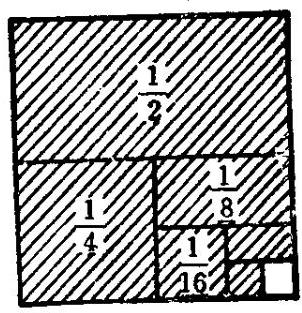
\includegraphics[max width=0.3\textwidth]{images/01912c18-5c3f-733d-b775-749ba9897a9d_14_791114.jpg}
\end{center}

图 1-3

上述结果可从图 1-3 中看出, 图 1-3 中各小矩形与小正

方形面积的和 (阴影部分) 的极限等于大正方形的面积.

例 3 中的无穷等比数列有这样的特点: 它的公比的绝对值小于 1 .

一般地, 设无穷等比数列

\[
{a}_{1},{a}_{1}q,{a}_{1}{q}^{2},\cdots ,{a}_{1}{q}^{n - 1},\cdots
\]

的公比 \(q\) 的绝对值小于 1,我们来求它的前 \(n\) 项的和当 \(n\) 无限增大时的极限.

无穷等比数列前 \(n\) 项的和是

\[
{S}_{n} = {a}_{1} + {a}_{1}q + \cdots + {a}_{1}{q}^{n - 1} = \frac{{a}_{1}\left( {1 - {q}^{n}}\right) }{1 - q},
\]

因此,

\[
\mathop{\lim }\limits_{{n \rightarrow \infty }}{S}_{n} = \mathop{\lim }\limits_{{n \rightarrow \infty }}\frac{{a}_{1}\left( {1 - {q}^{n}}\right) }{1 - q}
\]

\[
= \mathop{\lim }\limits_{{n \rightarrow \infty }}\frac{{a}_{1}}{1 - q} \cdot \mathop{\lim }\limits_{{n \rightarrow \infty }}\left( {1 - {q}^{n}}\right)
\]

\[
= \frac{{a}_{1}}{1 - q}\left( {\mathop{\lim }\limits_{{n \rightarrow \infty }}1 - \mathop{\lim }\limits_{{n \rightarrow \infty }}{q}^{n}}\right) .
\]

因为当 \(\left| q\right| < 1\) 时, \(\mathop{\lim }\limits_{{n \rightarrow \infty }}{q}^{n} = 0\) (证明较繁,本书从略),所以,

\[
\mathop{\lim }\limits_{{n \rightarrow \infty }}{S}_{n} = \frac{{a}_{1}}{1 - q} \cdot \left( {1 - 0}\right) = \frac{{a}_{1}}{1 - q}.
\]

公比的绝对值小于 1 的无穷等比数列前 \(n\) 项的和当 \(n\) 无限增大时的极限, 叫做这个无穷等比数列各项的和(注意: 这与有限个数的和从意义上说是不一样的),并且用符号 \(S\) 表示. 从上面知道,

\[
S = {a}_{1} + {a}_{1}q + {a}_{1}{q}^{2} + \cdots + {a}_{1}{q}^{n - 1} + \cdots = \frac{{a}_{1}}{1 - q}.
\]

例 4 求无穷等比数列 \({0.3},{0.03},{0.003},\cdots\) 各项的和.

解: \(\because {a}_{1} = {0.3},q = {0.1}\) ,

\[
\therefore \;S = \frac{0.3}{1 - {0.1}} = \frac{1}{3}\text{. }
\]

例 5 将下列循环小数化成分数:

(1) 0.7 ; (2) 0.231 .

解: (1) 纯循环小数 \({0.7} = {0.777}\cdots\) 可以写成

\[
\frac{7}{10} + \frac{7}{100} + \frac{7}{1000} + \cdots
\]

这里各项组成公比等于 \(\frac{1}{10}\) 的无穷等比数列,因此,

\[
{0.7} = \frac{\frac{7}{10}}{1 - \frac{1}{10}} = \frac{\frac{7}{10}}{\frac{9}{10}} = \frac{7}{9}
\]

也就是说, \({0.7} = \frac{7}{9}\) .

(2)混循环小数 \({0.231} = {0.2313131}\cdots\) 可以写成

\[
\frac{2}{10} + \frac{31}{1000} + \frac{31}{100000} + \frac{31}{10000000} + \cdots ,
\]

这里从第 2 项起各项组成公比等于 \(\frac{1}{100}\) 的无穷等比数列, 因此,

\[
{0.2}\dot{3}\dot{1} = \frac{2}{10} + \frac{\frac{31}{1000}}{1 - \frac{1}{100}} = \frac{2}{10} + \frac{31}{990}
\]

\[
= \frac{2 \times {99} + {31}}{990} = \frac{229}{990}
\]

\begin{problemset}[练习]
\item 已知 \(\mathop{\lim }\limits_{{n \rightarrow \infty }}{a}_{n} = 2,\mathop{\lim }\limits_{{n \rightarrow \infty }}{b}_{n} = - \frac{1}{3}\) ,求下列极限:

(1) \(\mathop{\lim }\limits_{{n \rightarrow \infty }}\left( {2{a}_{n} + 3{b}_{n}}\right)\) ; (2) \(\mathop{\lim }\limits_{{n \rightarrow \infty }}\frac{{a}_{n} - {b}_{n}}{{a}_{n}}\) .

\item 求下列极限:

(1) \(\mathop{\lim }\limits_{{n \rightarrow \infty }}\left( {3 - \frac{1}{n}}\right)\) (2) \(\mathop{\lim }\limits_{{n \rightarrow \infty }}\frac{2}{5 + \frac{3}{n}}\)

(3) \(\mathop{\lim }\limits_{{n \rightarrow \infty }}\frac{n + 1}{n}\) (4) \(\mathop{\lim }\limits_{{n \rightarrow \infty }}\frac{n - 1}{{n}^{2} + 1}\) .

\item 求下列无穷等比数列各项的和:

(1) \(3,1,\frac{1}{3},\frac{1}{9},\cdots\) ; (2) \(1, - \frac{1}{2},\frac{1}{4}, - \frac{1}{8},\cdots\) .

\end{problemset}
\begin{problemset}[习题一]
	\item 已知无穷数列 \(5 + 1,5 - \frac{1}{2},5 + \frac{1}{3},5 - \frac{1}{4},\cdots\) .
	
	(1)把这个数列的前 5 项在数轴上表示出来.
	
	(2)计算这个数列的第 \(n\) 项与 5 的差的绝对值 \(\left| {{a}_{n} - 5}\right|\) .
	
	(3)对于任何预先指定的正数 \(\varepsilon\) ,找一个自然数 \(N\) ,使得 \(n > N\) 时, \(\left| {{a}_{n} - 5}\right| < \varepsilon\) .
	
	(4)确定这个数列的极限。
	
	\item 一个无穷数列的通项公式是 \({a}_{n} = \frac{n + 1}{n + 2}\) .
	
	(1)把这个数列的前 5 项在数轴上表示出来。
	
	(2)计算 \(\left| {{a}_{n} - 1}\right|\) .
	
	(3)对于下表中的 \(\varepsilon\) ,各找出一个对应的自然数 \(N\) ,使得 \(n > N\) 时, \(\left| {{a}_{n} - 1}\right| < \varepsilon\) .
	
	\begin{center}
		\adjustbox{max width=\textwidth}{
			\begin{tabular}{|c|c|c|c|c|c|}
				\hline
				e & 0.2 & 0.1 & 0.05 & 0.01 & 任何给定 的正数 \\
				\hline
				\(N\) & \phantom{X} & \phantom{X} & \phantom{X} & \phantom{X} & \phantom{X} \\
				\hline
			\end{tabular}
		}
	\end{center}
	
	(4)确定这个数列的极限.
	
	\item 一个无穷数列的通项公式是 \({a}_{n} = \frac{{8n} + 1}{2n}\) .
	
	(1)把这个数列的前 5 项在数轴上表示出来.
	
	(2)计算 \(\left| {{a}_{n} - 4}\right|\) .
	
	(3)确定这个无穷数列的极限。
	
	\item 一个无穷数列的通项公式是 \({a}_{n} = \frac{n}{{2n} + 1}\) ,求证这个数列的极限是 \(\frac{1}{2}\) 。
	
	\item 举一个极限是 5 的无穷数列的例子.
	
	\item 无穷数列 \(- 2,0, - 2,0,\cdots ,{\left( -1\right) }^{n} - 1,\cdots\) 有极限吗?
	
	\item 已知无穷数列
	
	\[
	\frac{5}{3},\frac{10}{4},\frac{15}{5},\cdots ,\frac{5n}{n + 2},\cdots
	\]
	
	\[
	\frac{1}{3},\frac{2}{4},\frac{3}{5},\cdots ,\frac{n}{n + 2},\cdots
	\]
	
	(1)求证这两个数列的极限分别是 5 与 1 .
	
	(2)另作一个每一项都等于这两个数列的对应项的和的无穷数列. 验证所得数列的极限等于这两个数列的极限的和。
	
	\item 求下列极限:
	
	(1) \(\mathop{\lim }\limits_{{n \rightarrow \infty }}\left( {\frac{3}{{n}^{2}} + \frac{1}{n} + 5}\right)\) ; (2) \(\mathop{\lim }\limits_{{n \rightarrow \infty }}\frac{{2n} + 1}{{2n} - 1}\)
	
	(3) \(\mathop{\lim }\limits_{{n \rightarrow \infty }}\left( {\frac{2}{n} + \frac{{4n} - 1}{4n}}\right)\) (4) \(\mathop{\lim }\limits_{{n \rightarrow \infty }}\left( {1 - \frac{2n}{n + 2}}\right)\) ;
	
	(5) \(\mathop{\lim }\limits_{{n \rightarrow \infty }}\frac{5 + {7n}}{{6n} - {11}}\) (6) \(\mathop{\lim }\limits_{{n \rightarrow \infty }}\frac{2{n}^{2} + n - 1}{3{n}^{2} - 1}\)
	
	(7) \(\mathop{\lim }\limits_{{n \rightarrow \infty }}\frac{n + 1}{{n}^{2} - 9}\) (8) \(\mathop{\lim }\limits_{{n \rightarrow \infty }}\frac{{n}^{2} + n + 1}{{\left( n - 1\right) }^{2}}\) .
	
	\item (1) 求 \(\mathop{\lim }\limits_{{n \rightarrow \infty }}\frac{1 + 2 + \cdots + n}{{n}^{2}}\)
	
	(2)求 \(\mathop{\lim }\limits_{{n \rightarrow \infty }}\frac{{1}^{2} + {2}^{2} + \cdots + {n}^{2}}{{n}^{3}}\) .
	
	\[
	\text{(提示:}{1}^{2} + {2}^{2} + \cdots + {n}^{2} = \frac{n\left( {n + 1}\right) \left( {{2n} + 1}\right) }{6}\text{.}
	\]
	
	\item (1) 如图,在圆的内接正多边形中, \({r}_{n}\) 是边心距, \({p}_{n}\) 是周长, \({S}_{n}\) 是面积,求证 \({S}_{n} = \frac{1}{2}{p}_{n}{r}_{n}\) .
	
	(2)当圆的内接正多边形的边数无限增加时, \({r}_{n}\) 的极限是圆的半径 \(R,{p}_{n}\) 的极限是圆周长 \({2\pi R},{S}_{n}\) 的极限是圆面积,求证圆面积等于 \(\pi {R}^{2}\) .
	
	\item 如图,三角形的一条底边是 \(a\) ,这条边上的高是 \(h\) .
	
	(1)过高的 5 等分点分别作底边的平行线, 并作出相应的 4 个矩形, 求这些矩形面积的和.
	
	(2)把高 \(n\) 等分,同样作出 \(n - 1\) 个矩形,求这些矩形面积的和.
	
	(3)求证: 当 \(n\) 无限增大时,这些矩形面积的和的极限等于三角形的面积 \(\frac{ah}{2}\) .
	
	\begin{center}
		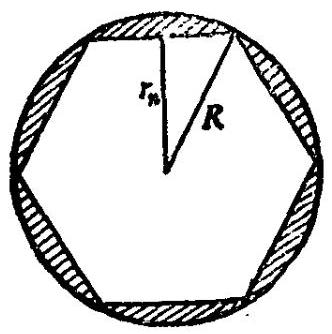
\includegraphics[max width=0.3\textwidth]{images/01912c18-5c3f-733d-b775-749ba9897a9d_20_155049.jpg}
	\end{center}
	
	(第 10 题)
	
	\begin{center}
		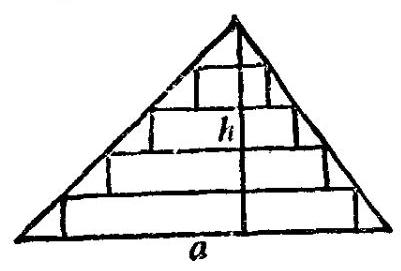
\includegraphics[max width=0.4\textwidth]{images/01912c18-5c3f-733d-b775-749ba9897a9d_20_862371.jpg}
	\end{center}
	
	(第 11 题)
	
	\item 求下列无穷等比数列各项的和:
	
	(1) \(\frac{8}{9}, - \frac{2}{3},\frac{1}{2}, - \frac{3}{8},\cdots\) ;
	
	(2) \(6\frac{2}{3},1\frac{1}{3},\frac{4}{15},\frac{4}{75},\cdots\) ;
	
	(3) \(\frac{\sqrt{3} + 1}{\sqrt{3} - 1},1,\frac{\sqrt{3} - 1}{\sqrt{3} + 1},\cdots\) ;
	
	(4) \(1, - x,{x}^{2}, - {x}^{3},\cdots ,\left( {\left| x\right| < 1}\right)\) .
	
	\item 如图,等边三角形 \({ABC}\) 的面积等于 1,连结这个三角形各边的中点得到一个小三角形, 又连结这个小三角形各边的中点得到一个更小的三角形, 如此无限继续下去, 求所有这些三角形面积的和。
	
	\begin{center}
		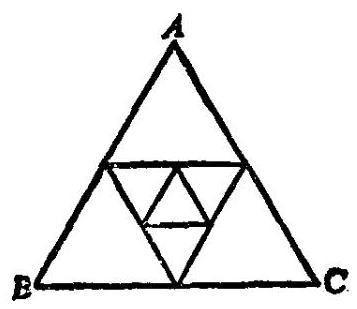
\includegraphics[max width=0.4\textwidth]{images/01912c18-5c3f-733d-b775-749ba9897a9d_20_529798.jpg}
	\end{center}
	
	(第 13 题)
	
	\begin{center}
		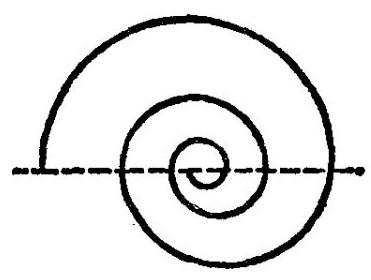
\includegraphics[max width=0.4\textwidth]{images/01912c18-5c3f-733d-b775-749ba9897a9d_20_500122.jpg}
	\end{center}
	
	(第 14 题)
	
	\item 如图, 第 1 个半圆的直径是 3 厘米, 第 2 个半圆的直径是
	
	2 厘米,以后每个半圆的直径都是前一个的 \(\frac{2}{3}\) ,这样无限继续下去, 求整条曲线的长。
	
	\item 将下列循环小数化成分数:
	
	(1) \({0.4}\) ; (2) 0.135 ;
	
	(3) \({0.436}\) ; (4) 2.138 .
	
\end{problemset}

\section{函数的极限}
前面我们研究了数列的极限的概念和极限的运算法则. 从本节起, 我们将讨论函数的极限的概念和运算法则.

\section*{1.当 \(x \rightarrow \infty\) 时函数的极限}


我们考察函数 \(y = \frac{1}{x}\) 当 \(x\) 无限增大时的变化趋势. 为此,

我们列出下表,并作出函数 \(y = \frac{1}{x}\) 的图象 (图 1-4).

\begin{center}
	\adjustbox{max width=\textwidth}{
		\begin{tabular}{|c|c|c|c|c|c|c|c|}
			\hline
			\(x\) & 1 & 10 & 100 & 1000 & 10000 & 100000 & 母曲曲 \\
			\hline
			\(y\) & 1 & 0.1 & 0.01 & 0.001 & 0.0001 & 0.00001 & ... \\
			\hline
		\end{tabular}
	}
\end{center}

从函数 \(y = \frac{1}{x}\) 的图象可以看出,当自变量 \(x\) 取正值并无限增大时,函数 \(y = \frac{1}{x}\) 的值无限趋近于零. 这里的“无限趋近于零”,就是表示函数值 \(y\) 与 0 之差的绝对值 \(\left| {y - 0}\right|\) 可以变得任意小.

\begin{center}
	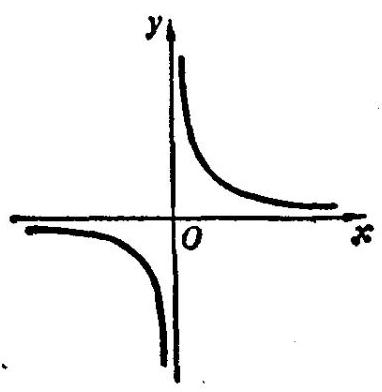
\includegraphics[max width=0.4\textwidth]{images/01912c18-5c3f-733d-b775-749ba9897a9d_21_654074.jpg}
\end{center}

图 1-4

例如,当 \(x\) 大于 1000 时,

\[
\left| {y - 0}\right| < {0.001}\text{.}
\]

当 \(x\) 大于 100000 时,

\[
\left| {y - 0}\right| < {0.00001}\text{.}
\]

一般地,对于预先指定的任意小的正数 \(\varepsilon\) ,当 \(x > \frac{1}{\varepsilon }\) 时,

\[
\left| {y - 0}\right| = \frac{1}{x} < \varepsilon
\]

总之,当 \(x\) 取正值并无限增大时,函数 \(y = \frac{1}{x}\) 的值无限趋近于 0 . 于是我们说,当 \(x\) 趋向于正无穷大时,函数 \(y = \frac{1}{x}\) 的极限是 0 , 记作

\[
\mathop{\lim }\limits_{{x \rightarrow + \infty }}\frac{1}{x} = 0
\]

同样地,当 \(x\) 取负值并且它的绝对值无限增大时,函数 \(y = \frac{1}{x}\) 的值也无限趋近于 0 . 于是我们说,当 \(x\) 趋向于负无穷大时,函数 \(y = \frac{1}{x}\) 的极限是 0,记作.

\[
\mathop{\lim }\limits_{{x \rightarrow - \infty }}\frac{1}{x} = 0
\]

一般地,当自变量 \(x\) 的绝对值无限增大时,如果函数 \(f\left( x\right)\) 无限趋近于一个常数 \(A\) ,就说当 \(x\) 趋向于无穷大时,函数 \(f\left( x\right)\) 的极限是 \(A\) ,记作

\[
\mathop{\lim }\limits_{{x \rightarrow \infty }}f\left( x\right) = A
\]

也可记作

当 \(x \rightarrow \infty\) 时, \(f\left( x\right) \rightarrow A\) .

\section*{2.当 \(x \rightarrow {x}_{0}\) 时函数的极限}


我们来研究函数 \(y = {x}^{2}\) 当 \(x\) 无限趋近于 2 时的变化趋势.

先列出下表,并作出函数 \(y = {x}^{2}\) 的图象 (图 1-5).

\begin{center}
	\adjustbox{max width=\textwidth}{
		\begin{tabular}{|c|c|c|c|c|c|c|}
			\hline
			\(x\) & 1. 5 & 1.9 & 1.99 & 1.999 & 1. 9999 & ... \\
			\hline
			\(y\) & 2. 25 & 3. 61 & 3.96 & 3.996 & 3 9996 & ... \\
			\hline
			\(\left| {y - 4}\right|\) & 1.75 & 0.39 & 0.04 & 0.004 & 0.0004 & es \\
			\hline
		\end{tabular}
	}
\end{center}

\begin{center}
	\adjustbox{max width=\textwidth}{
		\begin{tabular}{|c|c|c|c|c|c|c|}
			\hline
			\(x\) & 2. 5 & 2. 1 & 2.01 & 2.001 & 2.0001 & ... \\
			\hline
			\(y\) & 6.25 & 4.41 & 4.04 & 4.004 & 4.0004 & * \(* *\) \\
			\hline
			\(\left| {y - 4}\right|\) & 2. 25 & 0.41 & 0.04 & 0.004 & 0.0004 & . \\
			\hline
		\end{tabular}
	}
\end{center}

我们看到,当自变量 \(x\) 越接近 2 时,函数 \(y = {x}^{2}\) 的值越接近 4; 当 \(x\) 无限趋近于 2 (但不等于 2 ) 时, \(y\) 的值无限趋近于 4 . 于是我们说,当 \(x\) 无限趋近于 2 时,函数 \(y = {x}^{2}\) 的极限是 4,记作

\[
\mathop{\lim }\limits_{{x \rightarrow 2}}{x}^{2} = 4\text{. }
\]

\begin{center}
	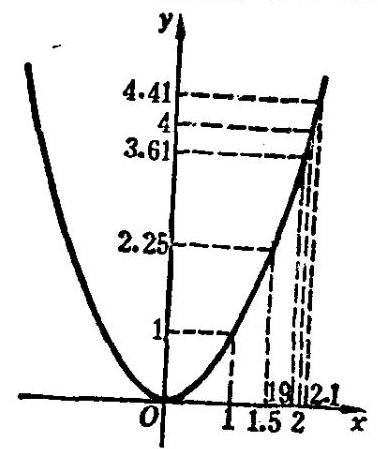
\includegraphics[max width=0.4\textwidth]{images/01912c18-5c3f-733d-b775-749ba9897a9d_23_174405.jpg}
\end{center}

图 1-5

我们再来研究函数 \(y = \frac{{x}^{2} - 1}{x - 1}\) 当 \(x\) 无限趋近于 1 (但不等 1)时的变化趋势.

如图 1-6,函数的图象是直线 \(y = x + 1\) 上除去点 \(\left( {1,2}\right)\) 以外的部分. 从图象上看到,当 \(x\) 接近于 1 时,函数 \(y = \frac{{x}^{2} - 1}{x - 1}\) 的值趋近于 2 .

\begin{center}
	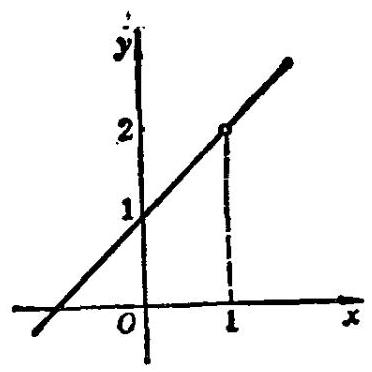
\includegraphics[max width=0.4\textwidth]{images/01912c18-5c3f-733d-b775-749ba9897a9d_24_728399.jpg}
\end{center}

图 1-6

这时,我们说,当 \(x\) 无限趋近于 1 (但不等于 1 ) 时, 函数

\[
y = \frac{{x}^{2} - 1}{x - 1}
\]

的极限是 2 , 记作

\[
\mathop{\lim }\limits_{{x \rightarrow 1}}\frac{{x}^{2} - 1}{x - 1} = 2
\]

一般地,当自变量 \(x\) 无限趋近于常数 \({x}_{0}\) (但 \(x\) 不等于 \({x}_{0}\) ) 时,如果函数 \(y = f\left( x\right)\) 无限趋近于一个常数 \(A\) ,就说当 \(x\) 趋近于 \({x}_{0}\) 时,函数 \(f\left( x\right)\) 的极限是 \(A\) ,记作

\[
\mathop{\lim }\limits_{{x \rightarrow {x}_{0}}}f\left( x\right) = A
\]

或者

当 \(x \rightarrow {x}_{0}\) 时, \(f\left( x\right) \rightarrow A\) .

从这个定义可以得出:

当 \(x\) 趋于任何数 \({x}_{0}\) 时,常数函数的极限就是这个常数, 即

\[
\mathop{\lim }\limits_{{x \rightarrow {x}_{0}}}C = C\text{. }
\]

当 \(x \rightarrow {x}_{0}\) 时, \(f\left( x\right) = x\) 的极限是 \({x}_{0}\) ,即

\[
\mathop{\lim }\limits_{{x \rightarrow {x}_{0}}}x = {x}_{0}
\]

\section*{3.函数的左极限和右极限}

首先,我们介绍在微积分中常常用到的函数 \(y = \left\lbrack x\right\rbrack\) ,符号 \(\left\lbrack x\right\rbrack\) 表示不超过数 \(x\) 的整数部分,例如

\[
\left\lbrack 0\right\rbrack = 0,\left\lbrack \frac{10}{3}\right\rbrack = \left\lbrack {{3.33}\cdots \cdots }\right\rbrack = 3,\;\left\lbrack {-{2.5}}\right\rbrack = - 3.
\]

函数 \(y = \left\lbrack x\right\rbrack\) 的图象如图 1-7.

现在,我们再来研究函数 \(y = \left\lbrack x\right\rbrack\) 在点 \(x = 1\) 处的极限.

如图 1-7,当 \(x\) 从点 \(x = 1\) 的左侧趋近于 1 时,函数 \(y\) 趋近于 0 ; 当 \(x\) 从点 \(x = 1\) 的右侧趋近于 1 时,函数 \(y\) 趋近于 1 . 因此,当 \(x\) 从点 \(x = 1\) 的左侧和右侧分别趋近于 1 时,函数 \(y\) 所趋近的值不同. 根据函数在一点处的极限的定义,函数 \(y\) 的极限不存在.

\begin{center}
	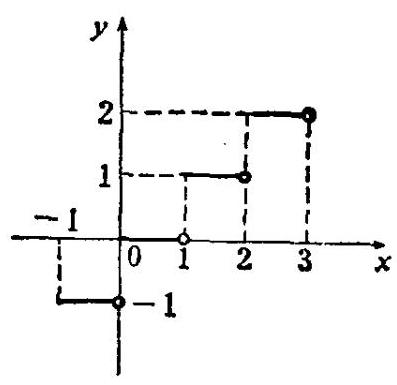
\includegraphics[max width=0.4\textwidth]{images/01912c18-5c3f-733d-b775-749ba9897a9d_25_214056.jpg}
\end{center}

图 1-7

从这个例子我们看到,虽然函数 \(y = \left\lbrack x\right\rbrack\) 在点 \(x = 1\) 处没有极限,但是当 \(x\) 从点 \(x = 1\) 的一侧趋近于 1 时,函数 \(y\) 还是趋近于确定的常数. 由此我们引出单侧极限的定义.

如果当 \(x\) 从点 \(x = {x}_{0}\) 左侧 (即 \(x < {x}_{0}\) ) 无限趋近于 \({x}_{0}\) 时,函数 \(f\left( x\right)\) 无限趋近于常数 \(A\) ,就说 \(A\) 是函数 \(f\left( x\right)\) 在点 \({x}_{0}\) 处的左极限, 记作

\[
\mathop{\lim }\limits_{{x \rightarrow {x}_{0} - }}f\left( x\right) = A\text{. }
\]

同样,如果当 \(x\) 从点 \(x = {x}_{0}\) 右侧 (即 \(x > {x}_{0}\) ) 无限趋近于 \({x}_{0}\) 时,函数 \(f\left( x\right)\) 无限趋近于常数 \(A\) ,就说 \(A\) 是函数 \(f\left( x\right)\) 在点 \({x}_{0}\) 处的右极限, 记作

\[
\mathop{\lim }\limits_{{x \rightarrow {x}_{0} + }}f\left( x\right) = A.
\]

根据极限、左极限和右极限的定义, 可以得出表示它们之间的关系的一条定理 (证明从略):

定理 \(\mathop{\lim }\limits_{{x \rightarrow {x}_{0}}}f\left( x\right) = A\) 的充要条件是

\[
\mathop{\lim }\limits_{{x \rightarrow {x}_{0} + }}f\left( x\right) = \mathop{\lim }\limits_{{x \rightarrow {x}_{0} - }}f\left( x\right) = A.
\]

\begin{problemset}[练习]
	\item 给定函数 \(y = \frac{1}{{x}^{2} + 1}\) . 填写下表并画出函数的图象,观察函数 \(y\) 当 \(x \rightarrow \infty\) 时的变化趋势:
	
	\begin{center}
		\adjustbox{max width=\textwidth}{
			\begin{tabular}{|c|c|c|c|c|c|c|}
				\hline
				\(x\) & 0 & \(\pm 2\) & \(\pm {10}\) & \(\pm {10}^{2}\) & \(\pm {10}^{3}\) & est \\
				\hline
				\(y\) & \phantom{X} & \phantom{X} & \phantom{X} & \phantom{X} & \phantom{X} & \phantom{X} \\
				\hline
				\(\left| {y - 0}\right|\) & \phantom{X} & \phantom{X} & \phantom{X} & \phantom{X} & \phantom{X} & \phantom{X} \\
				\hline
			\end{tabular}
		}
	\end{center}
	
	\item 根据函数极限的定义和函数的图象, 说出下列极限:
	
	(1) \(\mathop{\lim }\limits_{{x \rightarrow + \infty }}\frac{1}{{x}^{3}}\) (2) \(\mathop{\lim }\limits_{{x \rightarrow - \infty }}\frac{1}{{x}^{3}}\) (3) \(\mathop{\lim }\limits_{{x \rightarrow \infty }}\frac{1}{{x}^{3}}\) .
	
	\item 对于函数 \(y = {2x} + 1\) 填写下表,并作出函数的图象,观察当 \(x \rightarrow 1\) 时函数 \(y = {2x} + 1\) 的变化趋势:
	
	\begin{center}
		\adjustbox{max width=\textwidth}{
			\begin{tabular}{|c|c|c|c|c|c|c|}
				\hline
				\(x\) & 0.5 & 0.9 & 0.99 & 0.999 & 0.9999 & 0.99999 \\
				\hline
				\(y\) & \phantom{X} & \phantom{X} & \phantom{X} & \phantom{X} & \phantom{X} & \phantom{X} \\
				\hline
				\(\left| {y - 3}\right|\) & \phantom{X} & \phantom{X} & \phantom{X} & \phantom{X} & \phantom{X} & \phantom{X} \\
				\hline
			\end{tabular}
		}
	\end{center}
	
	\begin{center}
		\adjustbox{max width=\textwidth}{
			\begin{tabular}{|c|c|c|c|c|c|c|}
				\hline
				\(x\) & 1. 5 & 1. 1 & 1.01 & 1.001 & 1.0001 & 1.00001 \\
				\hline
				\(y\) & \phantom{X} & \phantom{X} & \phantom{X} & \phantom{X} & \phantom{X} & \phantom{X} \\
				\hline
				\(\left| {y - 3}\right|\) & \phantom{X} & \phantom{X} & \phantom{X} & \phantom{X} & \phantom{X} & \phantom{X} \\
				\hline
			\end{tabular}
		}
	\end{center}
	
	(1)当 \(\left| {x - 1}\right| < {0.01}\) 时, \(\left| {y - 3}\right|\) 小于什么数? 当 \(\left| {x - 1}\right|\) \(< {0.00001}\) 时, \(\left| {y - 3}\right|\) 小于什么数?
	
	(2)说出当 \(x \rightarrow 1\) 时函数 \(y\) 的极限.
	
	\item 根据函数极限的定义和函数的图象, 说出下列函数的极限 (其中 \(C\) 是常数):
	
	(1) \(\mathop{\lim }\limits_{{x \rightarrow \infty }}C\) ; (2) \(\mathop{\lim }\limits_{{x \rightarrow 3}}C\) ;
	
	(3) \(\mathop{\lim }\limits_{{x \rightarrow \infty }}\frac{1}{{x}^{2}}\) (4) \(\mathop{\lim }\limits_{{x \rightarrow 2}}\frac{1}{{x}^{2}}\) .
	
	\item 说出下列各图中表示的函数在点 \(x = a\) 的左极限、右极限和极限 (如果存在的话):
	
	\begin{center}
		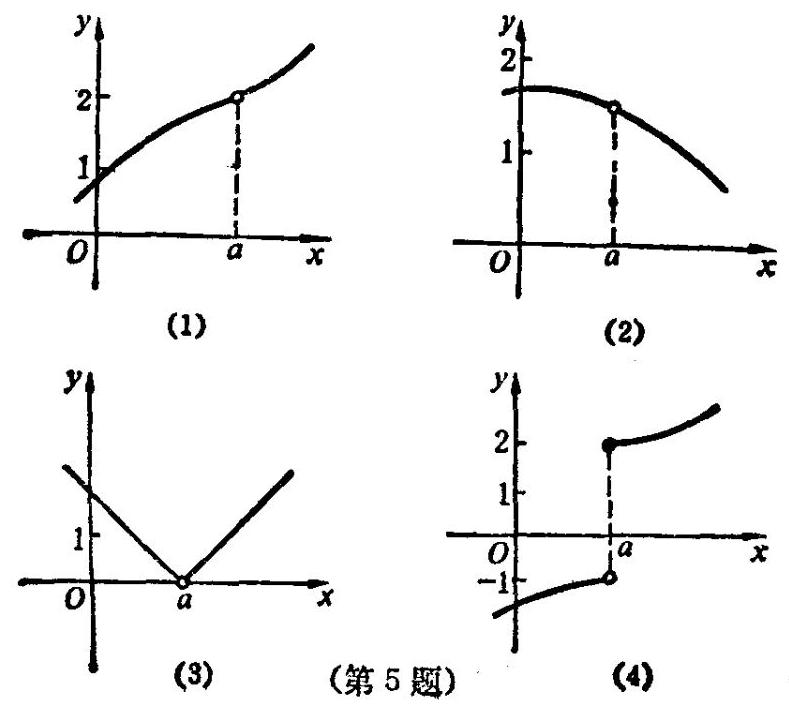
\includegraphics[max width=0.8\textwidth]{images/01912c18-5c3f-733d-b775-749ba9897a9d_27_586841.jpg}
	\end{center}
	
\end{problemset}

\section{函数极限的四则运算法则}

函数极限的四则运算与数列极限的四则运算有类似的定理.

如果 \(\mathop{\lim }\limits_{{x \rightarrow {x}_{0}}}f\left( x\right) = A,\mathop{\lim }\limits_{{x \rightarrow {x}_{0}}}g\left( x\right) = B\) ,那么,

\[
\mathop{\lim }\limits_{{x \rightarrow {x}_{0}}}\left\lbrack {f\left( x\right) \pm g\left( x\right) }\right\rbrack = A \pm B;
\]

\[
\mathop{\lim }\limits_{{x \rightarrow {x}_{0}}}\left\lbrack {f\left( x\right) \cdot \mathbf{g}\left( x\right) }\right\rbrack = \mathbf{A} \cdot \mathbf{B};
\]

\[
\mathop{\lim }\limits_{{x \rightarrow {x}_{0}}}\frac{f\left( x\right) }{g\left( x\right) } = \frac{A}{B}\left( {B \neq 0}\right) .
\]

这个定理对于 \(x \rightarrow \infty\) 的情况仍然成立.

由上面第二个式子可以推出: 当 \(C\) 是常数、 \(n\) 是正整数时,

\[
\mathop{\lim }\limits_{{x \rightarrow {x}_{0}}}\left\lbrack {{Cf}\left( x\right) }\right\rbrack = C\mathop{\lim }\limits_{{x \rightarrow {x}_{0}}}f\left( x\right) ;
\]

\[
\mathop{\lim }\limits_{{x \rightarrow {x}_{0}}}{\left\lbrack f\left( x\right) \right\rbrack }^{n} = {\left\lbrack \mathop{\lim }\limits_{{x \rightarrow {x}_{0}}}f\left( x\right) \right\rbrack }^{n}.
\]

利用函数极限的运算法则, 我们可以根据已知的几个函数的极限, 求出较复杂的函数的极限.

例 1 求 \(\mathop{\lim }\limits_{{x \rightarrow 2}}\left( {{x}^{2} + {3x}}\right)\) .

解: \(\mathop{\lim }\limits_{{x \rightarrow 2}}\left( {{x}^{2} + {3x}}\right) = \mathop{\lim }\limits_{{x \rightarrow 2}}{x}^{2} + \mathop{\lim }\limits_{{x \rightarrow 2}}{3x}\)

\[
= {\left( \mathop{\lim }\limits_{{x \rightarrow 2}}x\right) }^{2} + 3\mathop{\lim }\limits_{{x \rightarrow 2}}x
\]

\[
= {2}^{2} + 3 \times 2 = {10}\text{. }
\]

例 2 求 \(\mathop{\lim }\limits_{{x \rightarrow 1}}\frac{2{x}^{3} - {x}^{2} + 1}{x + 1}\) .

解: \(\mathop{\lim }\limits_{{x \rightarrow 1}}\frac{2{x}^{3} - {x}^{2} + 1}{x + 1} = \frac{\mathop{\lim }\limits_{{x \rightarrow 1}}\left( {2{x}^{3} - {x}^{2} + 1}\right) }{\mathop{\lim }\limits_{{x \rightarrow 1}}\left( {x + 1}\right) }\)

\[
= \frac{\mathop{\lim }\limits_{{x \rightarrow 1}}2{x}^{3} - \mathop{\lim }\limits_{{x \rightarrow 1}}{x}^{2} + \mathop{\lim }\limits_{{x \rightarrow 1}}1}{\mathop{\lim }\limits_{{x \rightarrow 1}}x + \mathop{\lim }\limits_{{x \rightarrow 1}}1}
\]

\[
= \frac{2{\left( \mathop{\lim }\limits_{{x \rightarrow 1}}x\right) }^{3} - {\left( \mathop{\lim }\limits_{{x \rightarrow 1}}x\right) }^{2} + \mathop{\lim }\limits_{{x \rightarrow 1}}1}{\mathop{\lim }\limits_{{x \rightarrow 1}}x + \mathop{\lim }\limits_{{x \rightarrow 1}}1}
\]

\[
= \frac{2 \times {1}^{3} - {1}^{2} + 1}{1 + 1}
\]

\[
= 1\text{.}
\]

例 3 求 \(\mathop{\lim }\limits_{{x \rightarrow 4}}\frac{{x}^{2} - {16}}{x - 4}\) .

分析: 当 \(x \rightarrow 4\) 时,分母的极限是 0,不能直接运用上面的极限运算法则. 因为当 \(x \rightarrow 4\) 时函数的极限,只与 \(x\) 无限趋近于 4 时的函数值有关,与 \(x = 4\) 时的函数值无关,因此可以先将分子和分母约去公因式 \(x - 4\) 以后再求函数的极限.

解: \(\mathop{\lim }\limits_{{x \rightarrow 4}}\frac{{x}^{2} - {16}}{x - 4} = \mathop{\lim }\limits_{{x \rightarrow 4}}\frac{\left( {x + 4}\right) \left( {x - 4}\right) }{x - 4}\)

\[
= \mathop{\lim }\limits_{{x \rightarrow 4}}\left( {x + 4}\right) = \mathop{\lim }\limits_{{x \rightarrow 4}}x + \mathop{\lim }\limits_{{x \rightarrow 4}}4
\]

\[
= 4 + 4 = 8\text{. }
\]

例 4 求 \(\mathop{\lim }\limits_{{x \rightarrow \infty }}\frac{3{x}^{2} - x + 2}{{x}^{2} + 1}\) .

分析: 当 \(x \rightarrow \infty\) 时,分子、分母没有极限,不能直接运用上面的商的极限运算法则. 为此,先将分子、分母同时除以 \({x}^{2}\) 后, 再求它的极限.

解: \(\mathop{\lim }\limits_{{x \rightarrow \infty }}\frac{3{x}^{2} - x + 2}{{x}^{2} + 1} = \mathop{\lim }\limits_{{x \rightarrow \infty }}\frac{\frac{3{x}^{2}}{{x}^{2}} - \frac{x}{{x}^{2}} + \frac{2}{{x}^{2}}}{\frac{{x}^{2}}{{x}^{2}} + \frac{1}{{x}^{2}}}\)

\[
= \frac{\mathop{\lim }\limits_{{x \rightarrow \infty }}\left( {3 - \frac{1}{x} + \frac{2}{{x}^{2}}}\right) }{\mathop{\lim }\limits_{{x \rightarrow \infty }}\left( {1 + \frac{1}{{x}^{2}}}\right) }
\]

\[
= \frac{\mathop{\lim }\limits_{{x \rightarrow \infty }}3 - \mathop{\lim }\limits_{{x \rightarrow \infty }}\frac{1}{x} + \mathop{\lim }\limits_{{x \rightarrow \infty }}\frac{2}{{x}^{2}}}{\mathop{\lim }\limits_{{x \rightarrow \infty }}1 + \mathop{\lim }\limits_{{x \rightarrow \infty }}\frac{1}{{x}^{2}}}
\]

\[
= \frac{\mathop{\lim }\limits_{{x \rightarrow \infty }}3 - \mathop{\lim }\limits_{{x \rightarrow \infty }}\frac{1}{x} + 2{\left( \mathop{\lim }\limits_{{x \rightarrow \infty }}\frac{1}{x}\right) }^{2}}{\mathop{\lim }\limits_{{x \rightarrow \infty }}1 + {\left( \mathop{\lim }\limits_{{x \rightarrow \infty }}\frac{1}{x}\right) }^{2}}
\]

\[
= \frac{3 - 0 + 0}{1 + 0} = 3\text{. }
\]

从以上各例求极限的过程可以看出, 在求有理函数的极限时, 最后总是归结为求下列极限:

\[
\mathop{\lim }\limits_{{x \rightarrow {x}_{0}}}C = C,\;\mathop{\lim }\limits_{{x \rightarrow {x}_{0}}}{x}^{k} = {x}_{0}^{k}\left( {k\text{ 是正整数 }}\right) ,
\]

\[
\mathop{\lim }\limits_{{x \rightarrow \infty }}C = C,\;\mathop{\lim }\limits_{{x \rightarrow \infty }}\frac{1}{{x}^{k}} = 0\text{ ( }k\text{ 是正整数). }
\]

这些极限可以由极限的定义和运算法则推出, 以后可以直接运用这些结果.

例 5 求 \(\mathop{\lim }\limits_{{x \rightarrow \infty }}\frac{2{x}^{2} + x - 4}{3{x}^{3} - {x}^{2} + 1}\) .

解: \(\mathop{\lim }\limits_{{x \rightarrow \infty }}\frac{2{x}^{2} + x - 4}{3{x}^{3} - {x}^{2} + 1} = \mathop{\lim }\limits_{{x \rightarrow \infty }}\frac{\frac{2{x}^{2}}{{x}^{3}} + \frac{x}{{x}^{3}} - \frac{4}{{x}^{3}}}{\frac{3{x}^{3}}{{x}^{3}} - \frac{{x}^{2}}{{x}^{3}} + \frac{1}{{x}^{3}}}\)

\[
= \frac{\mathop{\lim }\limits_{{x \rightarrow \infty }}\left( {\frac{2}{x} + \frac{1}{{x}^{2}} - \frac{4}{{x}^{3}}}\right) }{\mathop{\lim }\limits_{{x \rightarrow \infty }}\left( {3 - \frac{1}{x} + \frac{1}{{x}^{3}}}\right) }
\]

\[
= \frac{0 + 0 - 0}{3 - 0 + 0} = 0\text{. }
\]


\begin{problemset}[练习]
\item 利用函数极限的运算法则求下列极限:

(1) \(\mathop{\lim }\limits_{{x \rightarrow \frac{1}{2}}}\left( {{2x} - 3}\right)\) ; (2) \(\mathop{\lim }\limits_{{x \rightarrow 2}}\left( {2{x}^{2} - {3x} + 1}\right)\) ;

(3) \(\mathop{\lim }\limits_{{x \rightarrow 4}}\left( {{2x} - 1}\right) \left( {x + 3}\right)\) ; (4) \(\mathop{\lim }\limits_{{x \rightarrow 1}}\frac{2{x}^{2} + 1}{3{x}^{2} + {4x} - 1}\) .

\item 求下列极限:

(1) \(\mathop{\lim }\limits_{{x \rightarrow 3}}\frac{{x}^{2} - {5x} + 6}{{x}^{2} - 9}\) (2) \(\mathop{\lim }\limits_{{x \rightarrow - 1}}\frac{{x}^{3} + 1}{x + 1}\)

(3) \(\mathop{\lim }\limits_{{x \rightarrow \infty }}\frac{2{x}^{2} + x - 2}{3{x}^{2} - {3x} + 1}\) (4) \(\mathop{\lim }\limits_{{y \rightarrow \infty }}\frac{2{y}^{2} - y}{{y}^{3} - 5}\) .

\end{problemset}
\begin{problemset}[习 题 二]

\item 根据函数极限的定义, 说出下列极限:

(1) \(\mathop{\lim }\limits_{{x \rightarrow + \infty }}{\left( \frac{1}{2}\right) }^{x}\) (2) \(\mathop{\lim }\limits_{{x \rightarrow \infty }}\frac{2}{{x}^{2} + 1}\) .

\item 根据函数极限的定义, 说出下列极限:

(1) \(\mathop{\lim }\limits_{{x \rightarrow 2}}{3x}\) (2) \(\mathop{\lim }\limits_{{x \rightarrow a}}\left( {{2x} - 1}\right)\) ; 1

(3) \(\mathop{\lim }\limits_{{x \rightarrow - 1}}\frac{1}{{x}^{2}}\) (4) \(\mathop{\lim }\limits_{{x \rightarrow 1}}\frac{{x}^{3} - x}{x - 1}\) .

\item 求下列极限:

(1) \(\mathop{\lim }\limits_{{x \rightarrow 1}}\left( {2{x}^{3} + {3x} + 4}\right)\) ; (2) \(\mathop{\lim }\limits_{{x \rightarrow 2}}\frac{{x}^{2} + 5}{{x}^{2} - 3}\)

(3) \(\mathop{\lim }\limits_{{x \rightarrow 0}}\left( {\frac{{x}^{2} - {3x} + 1}{x - 4} + 1}\right)\) ; (4) \(\mathop{\lim }\limits_{{x \rightarrow \sqrt{3}}}\frac{{x}^{2} - 3}{{x}^{4} + {x}^{2} + 1}\)

(5) \(\mathop{\lim }\limits_{{x \rightarrow 2}}\frac{x - 2}{{x}^{3} - 8}\) (6) \(\mathop{\lim }\limits_{{x \rightarrow 1}}\frac{2x}{1 + x + {x}^{2}}\)

(7) \(\mathop{\lim }\limits_{{x \rightarrow 1}}\frac{{x}^{2} - {2x} + 1}{{x}^{3} - 1}\) (8) \(\mathop{\lim }\limits_{{x \rightarrow 0}}\frac{3{x}^{3} + {x}^{2}}{{x}^{5} + 3{x}^{4} - 2{x}^{2}}\)

(9) \(\mathop{\lim }\limits_{{x \rightarrow - 2}}\frac{{x}^{3} + 3{x}^{2} + {2x}}{{x}^{2} - x - 6}\) (10) \(\mathop{\lim }\limits_{{x \rightarrow 0}}\frac{{\left( x + m\right) }^{3} - {m}^{3}}{x}\)

(11) \(\mathop{\lim }\limits_{{x \rightarrow \infty }}\left( {2 - \frac{1}{x} + \frac{1}{{x}^{2}}}\right)\) (12) \(\mathop{\lim }\limits_{{x \rightarrow \infty }}\frac{{x}^{2} + 1}{2{x}^{2} + {2x} - 1}\)

(13) \(\mathop{\lim }\limits_{{x \rightarrow \infty }}\frac{{x}^{3} + x}{{x}^{4} + 3{x}^{2} + 1}\) (14) \(\mathop{\lim }\limits_{{x \rightarrow \infty }}{\left( \frac{2{x}^{3} + 1}{3{x}^{3} - 2}\right) }^{2}\) .

\item 求下列极限:

(1) \(\mathop{\lim }\limits_{{x \rightarrow 1}}\frac{3{x}^{2} - {11x} + 6}{2{x}^{2} - {5x} - 3}\) ; (2) \(\mathop{\lim }\limits_{{x \rightarrow \infty }}\frac{3{x}^{2} - {11x} + 6}{2{x}^{2} - {5x} - 3}\) ;

(3) \(\mathop{\lim }\limits_{{x \rightarrow 0}}\frac{x - {x}^{2} - 6{x}^{3}}{{2x} - 5{x}^{2} - 3{x}^{3}}\) ; (4) \(\mathop{\lim }\limits_{{x \rightarrow \infty }}\frac{x - {x}^{2} - 6{x}^{3}}{{2x} - 5{x}^{2} - 3{x}^{3}}\) .
\end{problemset}
\section{函数的连续性}
我们以前学过的许多函数,例如 \(y = {x}^{2}\) ,它的图象是连续 (不间断) 的曲线. 对于连续曲线 \(y = f\left( x\right)\) 上的每一点 \({x}_{0}\) 来说,当 \(x \rightarrow {x}_{0}\) 时,都有 \(f\left( x\right) \rightarrow f\left( {x}_{0}\right)\) .

如果函数 \(y = f\left( x\right)\) 在点 \({x}_{0}\) 的附近有定义,而且

\[
\mathop{\lim }\limits_{{x \rightarrow {x}_{0}}}f\left( x\right) = f\left( {x}_{0}\right)
\]

就说函数 \(f\left( x\right)\) 在点 \({x}_{0}\) 处连续.

例 1 研究函数 \(f\left( x\right) = {x}^{2}\) 在点 \(x = 2\) 处的连续性.

解: 函数 \(f\left( x\right) = {x}^{2}\) 在点 \(x = 2\) 的附近有定义,而且

\[
\mathop{\lim }\limits_{{x \rightarrow 2}}{x}^{2} = 4
\]

\[
f\left( 2\right) = {2}^{2} = 4,
\]

\(\therefore\)

\[
\mathop{\lim }\limits_{{x \rightarrow 2}}{x}^{2} = f\left( 2\right) \text{. }
\]

因此,函数 \(f\left( x\right) = {x}^{2}\) 在点 \(x = 2\) 处连续.

从上面的定义可以看出,函数 \(f\left( x\right)\) 在点 \(x = {x}_{0}\) 处连续必须具备以下三个条件:

1. 函数 \(f\left( x\right)\) 在点 \({x}_{0}\) 的附近有定义;

2. \(\mathop{\lim }\limits_{{x \rightarrow {x}_{0}}}f\left( x\right)\) 存在;

3. \(\mathop{\lim }\limits_{{x \rightarrow {x}_{0}}}f\left( x\right) = f\left( {x}_{0}\right)\) ,即函数 \(f\left( x\right)\) 在点 \({x}_{0}\) 处的极限等于 \(f\left( x\right)\) 在点 \({x}_{0}\) 的函数值.

如果函数 \(f\left( x\right)\) 在点 \(x = {x}_{0}\) 处对上述三个条件中有一个条件不具备,那么函数在点 \(x = {x}_{0}\) 处不连续,点 \(x = {x}_{0}\) 称为该函数的间断点.

例如,函数 \(y = \operatorname{tg}x\) 在点 \(x = \frac{\pi }{2}\) 处没有定义,所以 \(x = \frac{\pi }{2}\) 是函数 \(y = \operatorname{tg}x\) 的间断点.

下面我们给出函数 \(f\left( x\right)\) 在点 \({x}_{0}\) 处右连续和左连续的定义.

如果函数 \(f\left( x\right)\) 在点 \({x}_{0}\) 附近右侧 (或左侧) 有定义,而且

\[
\mathop{\lim }\limits_{{x \rightarrow {x}_{0} + }}f\left( x\right) = f\left( {x}_{0}\right) \text{ (或者 }\mathop{\lim }\limits_{{x \rightarrow {x}_{0} - }}f\left( x\right) = f\left( {x}_{0}\right) \text{ ),}
\]

那么就说函数 \(f\left( x\right)\) 在点 \(x\) 处右连续 (或者左连续),

例 2 研究函数 \(y = \left\lbrack x\right\rbrack\) 在点 \(x = 2\) 处的连续性.

解: 函数 \(y = \left\lbrack x\right\rbrack\) 在 \(x = 2\) 的附近有定义 (参看图 1-7).

由于

\[
\mathop{\lim }\limits_{{x \rightarrow 2 + }}\left\lbrack x\right\rbrack = 2 = \left\lbrack 2\right\rbrack ,\;\mathop{\lim }\limits_{{x \rightarrow 2 - }}\left\lbrack x\right\rbrack = 1 \neq \left\lbrack 2\right\rbrack ,
\]

所以函数 \(y = \left\lbrack x\right\rbrack\) 在点 \(x = 2\) 处是右连续,但不是左连续.

由于当 \(x \rightarrow 2\) 时函数 \(\left\lbrack x\right\rbrack\) 没有极限,所以函数 \(y = \left\lbrack x\right\rbrack\) 在点 \(x = 2\) 处不连续.

如果函数 \(f\left( x\right)\) 在某一区间 \(\left( {a,b}\right)\) 内每一点处都连续,就说 \(f\left( x\right)\) 在区间 \(\left( {\mathbf{a},\mathbf{b}}\right)\) 内连续,或者说 \(f\left( x\right)\) 是区间 \(\left( {\mathbf{a},\mathbf{b}}\right)\) 内的连续函数.

如果函数 \(f\left( x\right)\) 在开区间 \(\left( {a,b}\right)\) 内连续,在左端点 \(x = a\) 处右连续,在右端点 \(x = b\) 处左连续,就说函数 \(f\left( x\right)\) 在闭区间 \(\left\lbrack {a,b}\right\rbrack\) 上连续.

例如,函数 \(y = 1 - {x}^{2}\) 在闭区间 \(\left\lbrack {-1,1}\right\rbrack\) 上连续. 而函数 \(y = \frac{1}{x}\) 在开区间 \(\left( {0,1}\right)\) 内连续,在闭区间 \(\left\lbrack {0,1}\right\rbrack\) 上不连续,因为它在点 \(x = 0\) 不是右连续.

在区间上连续的函数的图象, 是一条连续的曲线. 利用闭区间上连续函数的图象可以说明它具有如下的性质.

\begin{center}
	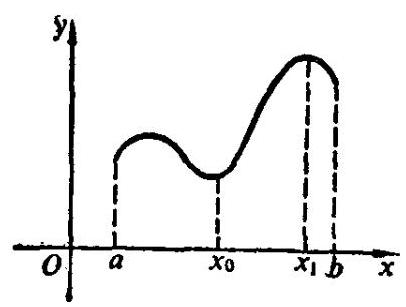
\includegraphics[max width=0.4\textwidth]{images/01912c18-5c3f-733d-b775-749ba9897a9d_34_898703.jpg}
\end{center}

图 1-8

性质 1 (最大值和最小值定理) 如果 \(f\left( x\right)\) 是闭区间 \(\left\lbrack {a,b}\right\rbrack\) 上的连续函数,那么 \(f\left( x\right)\) 在 \(\left\lbrack {a,b}\right\rbrack\) 上有最大值和最小值.

如图 1-8, \(f\left( {x}_{1}\right) \geq f\left( x\right) ,x \in \left\lbrack {a,b}\right\rbrack\) ;

\[
f\left( {x}_{0}\right) \leq f\left( x\right) ,\;x \in \left\lbrack {a,b}\right\rbrack .
\]

利用函数极限的运算法则, 还可以证明连续函数的和、 差、积、商仍然是连续函数.

性质 2 如果函数 \(f\left( x\right) \text{、}g\left( x\right)\) 在某一点 \(x = {x}_{0}\) 处连续, 那么

(1) \(f\left( x\right) \pm g\left( x\right)\) ,

(2) \(f\left( x\right) \cdot g\left( x\right)\) ,

(3) \(\frac{f\left( x\right) }{g\left( x\right) }\;\left( {g\left( x\right) \neq 0}\right)\)

在点 \(x = {x}_{0}\) 处都连续.

证明: 因为函数 \(f\left( x\right) \text{、}g\left( x\right)\) 在点 \(x = {x}_{0}\) 处连续,所以,

\[
\mathop{\lim }\limits_{{x \rightarrow {x}_{0}}}f\left( x\right) = f\left( {x}_{0}\right) ,\mathop{\lim }\limits_{{x \rightarrow {x}_{0}}}g\left( x\right) = g\left( {x}_{0}\right) .
\]

由极限的运算法则, 得出

\[
\mathop{\lim }\limits_{{x \rightarrow {x}_{0}}}\left\lbrack {f\left( x\right) \pm g\left( x\right) }\right\rbrack = \mathop{\lim }\limits_{{x \rightarrow {x}_{0}}}f\left( x\right) \pm \mathop{\lim }\limits_{{x \rightarrow {x}_{0}}}g\left( x\right)
\]

\[
= f\left( {x}_{0}\right) \pm g\left( {x}_{0}\right) \text{.}
\]

因此,函数 \(f\left( x\right) \pm g\left( x\right)\) 在点 \(x = {x}_{0}\) 处连续.

同样可以证明(2)和(3).

\begin{problemset}[练习]


\item 连续函数的图象有什么特点? 观察下列各函数图象, 说出函数在 \(x = a\) 处是否连续:

\begin{center}
	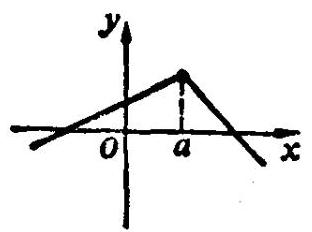
\includegraphics[max width=0.3\textwidth]{images/01912c18-5c3f-733d-b775-749ba9897a9d_35_115885.jpg}
	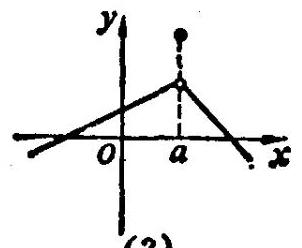
\includegraphics[max width=0.3\textwidth]{images/01912c18-5c3f-733d-b775-749ba9897a9d_35_560451.jpg}
	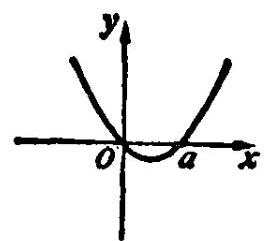
\includegraphics[max width=0.3\textwidth]{images/01912c18-5c3f-733d-b775-749ba9897a9d_35_351282.jpg}
\end{center}

\noindent % 确保表格从左边开始,不产生额外的缩进
\begin{tabular}{ccc}
	\makebox[0.3\textwidth][c]{(1)} &
	\makebox[0.3\textwidth][c]{(2)} &
	\makebox[0.3\textwidth][c]{(3)}
\end{tabular}

\begin{center}
	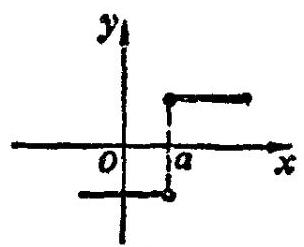
\includegraphics[max width=0.3\textwidth]{images/01912c18-5c3f-733d-b775-749ba9897a9d_36_706273.jpg}
	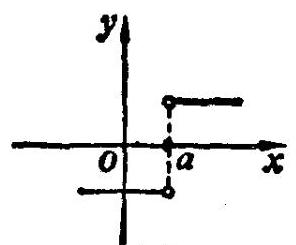
\includegraphics[max width=0.3\textwidth]{images/01912c18-5c3f-733d-b775-749ba9897a9d_36_222184.jpg}
	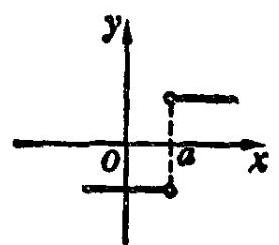
\includegraphics[max width=0.3\textwidth]{images/01912c18-5c3f-733d-b775-749ba9897a9d_36_774109.jpg}
\end{center}

\noindent % 确保表格从左边开始,不产生额外的缩进
\begin{tabular}{ccc}
	\makebox[0.3\textwidth][c]{(3)} &
	\makebox[0.3\textwidth][c]{(4)} &
	\makebox[0.3\textwidth][c]{(5)}
\end{tabular}

\begin{center}
	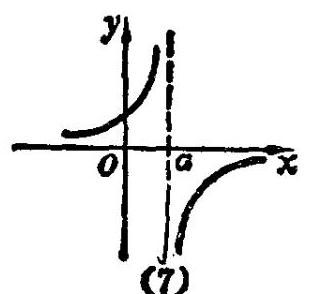
\includegraphics[max width=0.3\textwidth]{images/01912c18-5c3f-733d-b775-749ba9897a9d_36_255638.jpg}
	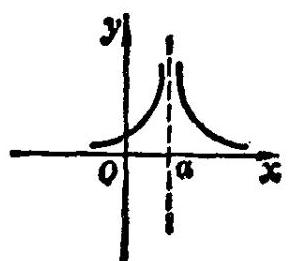
\includegraphics[max width=0.3\textwidth]{images/01912c18-5c3f-733d-b775-749ba9897a9d_36_333878.jpg}
	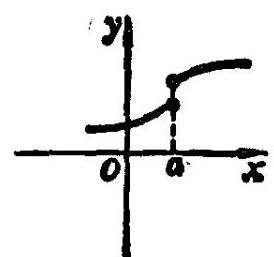
\includegraphics[max width=0.3\textwidth]{images/01912c18-5c3f-733d-b775-749ba9897a9d_36_561922.jpg}
\end{center}

\noindent % 确保表格从左边开始,不产生额外的缩进
\begin{tabular}{ccc}
	\makebox[0.3\textwidth][c]{(7)} &
	\makebox[0.3\textwidth][c]{(8)} &
	\makebox[0.3\textwidth][c]{(9)}
\end{tabular}


(第 1 题)

\item 结合下列函数的图象, 说明函数在给定点或区间上是否连续:

(1) \(f\left( x\right) = \frac{1}{{x}^{2}},x = 0\) ; (2) \(f\left( x\right) = \left| x\right| ,x = 0\) ;

(3) \(f\left( x\right) = \frac{{x}^{2} - 1}{x - 1},\left( {0,1}\right)\) ;

(4) \(f\left( x\right) = a{x}^{2} + {bx} + c,\left( {-\infty ,\infty }\right)\) .

\end{problemset}

\subsection*{复合函数的连续性}
我们学过的函数可以分为以下五类: .

幂函数 \(y = {x}^{\alpha }\) ( \(\alpha\) 是实数); 0.5

指数函数 \(y = {a}^{x}\left( {a > 0\text{,且}a \neq 1}\right)\) ;

对数函数 \(y = {\log }_{a}x\left( {a > 0\text{,且}a \neq 1}\right)\) ;

三角函数 \(y = \sin x,y = \cos x,y = \operatorname{tg}x,y = \operatorname{ctg}x\) ,等等;

反三角函数 \(y = \arcsin x,y = \arccos x,y = \operatorname{arctg}x\) ,

\(y = \operatorname{arcctg}x\) ,等等. 这五种函数统称基本初等函数.

关于基本初等函数的连续性有如下结论:

基本初等函数在其定义区间上是连续函数.

例如, \(y = {x}^{\frac{1}{2}}\) 在 \(\lbrack 0, + \infty )\) 上连续, \(y = \sin x\) 在 \(\left( {-\infty , + \infty }\right)\) 上连续, \(y = \operatorname{tg}x\) 在 \(\left( {{n\pi } - \frac{\pi }{2},{n\pi } + \frac{\pi }{2}}\right)\) 上连续.

我们以前学过的许多函数是由基本初等函数和常数经过有限次四则运算得出的. 例如, 二次函数

\[
y = a{x}^{2} + {bx} + c
\]

可以看作是由常数 \(a\) 乘以幂函数 \({x}^{2}\) 的积,加上常数 \(b\) 乘以幂函数 \(x\) 的积,再加上常数 \(c\) 而得到的一个函数.

另外还有一些函数,例如 \(y = \sin {2x}\) ,它和 \(y = \sin x\) 不同, 不是基本初等函数. 下面我们将会看到, 它是由三角函数 \(y = \sin u\) 和一次函数 \(u = {2x}\) 经过 “复合”而成的.

同样, 函数

\[
y = \sqrt{1 + {x}^{2}}
\]

是由幂函数 \(y = {u}^{\frac{1}{2}}\) 和二次函数 \(u = 1 + {x}^{2}\) 经过 “复合”而成的.

一般地说,如果 \(y\) 是 \(u\) 的函数,而 \(u\) 又是 \(x\) 的函数,即 \(y = f\left( u\right) ,u = g\left( x\right)\) ,那么 \(y\) 关于 \(x\) 的函数

\[
y = f\left\lbrack {g\left( x\right) }\right\rbrack
\]

叫做函数 \(f\) 和 \(g\) 的复合函数, \(u\) 叫做中间变量.

例 1 (1) 函数 \(y = f\left( u\right) = \lg u\) 与 \(u = g\left( x\right) = \sin x\) 经过 “复合”以后得到什么函数?

(2)函数 \(y = f\left( u\right) = \sin u\) 与 \(u = g\left( x\right) = \lg x\) 呢?

解: (1) \(\lg \sin x\) ;

(2) \(\sin \left( {\lg x}\right)\) .

复合函数也可以是由三个或三个以上的函数复合而成的.

例 2 说出下列函数是由哪几个简单的函数复合而成的:

(1) \(y = a\sin \left( {{bt} + c}\right)\) ;

(2) \(y = {\log }_{a}{\left( 1 + x\right) }^{2}\) .

解: (1) \(y = a\sin \left( {{bt} + c}\right)\) 可以看成是 \(y = a\sin u\) 和 \(u =\) \({bt} + c\) 两个函数复合而成的.

(2) \(y = {\log }_{a}{\left( 1 + x\right) }^{2}\) 可以看成是由 \(y = {\log }_{a}u,u = {v}^{2},v =\) \(1 + x\) 三个函数复合而成的.

一般地, 关于复合函数连续性有如下结论:

如果函数 \(u = g\left( x\right)\) 在点 \(x = {x}_{0}\) 处连续, \(g\left( {x}_{0}\right) = {u}_{0}\) ,且函数 \(y = f\left( u\right)\) 在点 \(u = {u}_{0}\) 处连续,那么复合函数 \(y = f\left\lbrack {g\left( x\right) }\right\rbrack\) 在点 \({x}_{0}\) 处连续.

由基本初等函数和常数经过有限次四则运算和有限次函数的复合而得出的函数, 统称初等函数.

由基本初等函数的连续性、连续函数的性质 2 和复合函数的连续性可以得出如下结论:

一切初等函数在它们的定义区间上是连续函数.

根据这条结论, 函数

\[
y = \frac{{ax} + b}{c{x}^{2} + d},\;y = a\sin \left( {{\omega t} + \varphi }\right) ,
\]

\[
y = {\log }_{a}{\left( 1 + x\right) }^{2},\;y = \sqrt{{a}^{2} - {b}^{2}{\cos }^{2}x},\;y = \frac{{e}^{x} - {e}^{-x}}{2}
\]

都是在其定义区间上的连续函数.

这个结论不仅给我们提供了判断一个函数是不是连续函数的根据, 而且为我们提供了计算初等函数的极限问题的一种方法. 这种方法是: 如果函数 \(f\left( x\right)\) 是初等函数,而且点 \({x}_{0}\) 是函数定义区间内的一点,那么求 \(x \rightarrow {x}_{0}\) 时函数 \(f\left( x\right)\) 的极限,只要求出 \(f\left( x\right)\) 在点 \({x}_{0}\) 处的函数值 \(f\left( {x}_{0}\right)\) 就可以了.

例 3 利用初等函数的连续性, 求下列极限:

(1) \(\mathop{\lim }\limits_{{x \rightarrow 1}}\sqrt{3 + {x}^{2}}\) ; (2) \(\mathop{\lim }\limits_{{x \rightarrow 0}}\frac{1 - {e}^{x}}{1 + {e}^{x}}\)

(3) \(\mathop{\lim }\limits_{{x \rightarrow \frac{\pi }{2}}}\ln \sin x\) ;

(4) \(\mathop{\lim }\limits_{{x \rightarrow a}}\sqrt{1 + {\operatorname{arctg}}^{2}\frac{x}{a}}\;\left( {a \neq 0}\right)\) .

解: (1) \(\mathop{\lim }\limits_{{x \rightarrow 1}}\sqrt{3 + {x}^{2}} = \sqrt{3 + {1}^{2}} = 2\) ;

(2) \(\mathop{\lim }\limits_{{x \rightarrow 0}}\frac{1 - {e}^{x}}{1 + {e}^{x}} = \frac{1 - {e}^{0}}{1 + {e}^{0}} = \frac{1 - 1}{1 + 1} = 0\) ;

(3) \(\mathop{\lim }\limits_{{x \rightarrow \frac{\pi }{2}}}\ln \sin x = \ln \sin \frac{\pi }{2} = \ln 1 = 0\) ;

(4) \(\mathop{\lim }\limits_{{x \rightarrow a}}\sqrt{1 + \operatorname{arctg}{}^{2}\frac{x}{a}} = \sqrt{1 + \operatorname{arctg}{}^{2}\frac{a}{a}}\)

\[
= \sqrt{1 + {\left( \frac{\pi }{4}\right) }^{2}}
\]

\[
= \frac{1}{4}\sqrt{{16} + {\pi }^{2}}
\]

例 4 求下列极限:

(1) \(\mathop{\lim }\limits_{{x \rightarrow 1}}\frac{\left( {x - 1}\right) \sqrt{2 - x}}{{x}^{4} - 1}\) ; (2) \(\mathop{\lim }\limits_{{x \rightarrow 0}}\frac{\sqrt{1 + x} - 1}{x}\) .

解: (1) \(\mathop{\lim }\limits_{{x \rightarrow 1}}\frac{\left( {x - 1}\right) \sqrt{2 - x}}{{x}^{4} - 1} = \mathop{\lim }\limits_{{x \rightarrow 1}}\frac{\sqrt{2 - x}}{{x}^{3} + {x}^{2} + x + 1}\)

\[
= \frac{\sqrt{2 - 1}}{{1}^{3} + {1}^{2} + 1 + 1}
\]

\[
= \frac{1}{4}\text{. }
\]

(2) \(\mathop{\lim }\limits_{{x \rightarrow 0}}\frac{\sqrt{1 + x} - 1}{x} = \mathop{\lim }\limits_{{x \rightarrow 0}}\frac{\left( {\sqrt{1 + x} - 1}\right) \left( {\sqrt{1 + x} + 1}\right) }{x\left( {\sqrt{1 + x} + 1}\right) }\)

\[
= \mathop{\lim }\limits_{{x \rightarrow 0}}\frac{x}{x\left( {\sqrt{1 + x} + 1}\right) }
\]

\[
= \mathop{\lim }\limits_{{x \rightarrow 0}}\frac{1}{\sqrt{1 + x} + 1} = \frac{1}{2}\text{. }
\]

\begin{problemset}[练习]

\item 下列函数是由基本初等函数经过哪些运算得出的函数?

(1) \(y = {ax} + b\) ; (2) \(y = \frac{1 + {x}^{2}}{ax}\) ;

(3) \(y = 5{a}^{x}\sin x\) ; (4) \(y = \left( {1 + \ln x}\right) \sin x\) .

\item 写出下列函数经过复合而成的函数的表示式:

(1) \(y = {e}^{u},u = {x}^{2}\) ; (2) \(y = {u}^{2},u = {e}^{x}\) ;

(3) \(y = \sqrt{u},u = 1 + {\sin }^{2}x\) ;

(4) \(y = a{u}^{2},u = \sin v,v = {bx} + c\) .

\item 说出下列函数是由哪几个简单的函数复合而成的:

(1) \(y = \sqrt{1 + {a}^{x}}\) ; (2) \(y = \ln {ax}\) ;

(3) \(y = \frac{1}{\cos \left( {1 + {x}^{2}}\right) }\) ; (4) \(y = \sqrt{{a}^{2} - {b}^{2}{\cos }^{2}x}\) .

\item 求下列极限:

(1) \(\mathop{\lim }\limits_{{x \rightarrow 0}}\lg \cos {3x}\) ; (2) \(\mathop{\lim }\limits_{{x \rightarrow \frac{\pi }{2}}}\frac{\sin {2x}}{\cos x}\)

(3) \(\mathop{\lim }\limits_{{x \rightarrow 1}}\frac{\sqrt{3 + {x}^{2}} - \sqrt{{x}^{2} - 1}}{x + 1}\)

(4) \(\mathop{\lim }\limits_{{x \rightarrow 0}}\frac{\left( {1 + {a}^{x}}\right) \left( {1 - \cos x}\right) }{{\sin }^{2}\frac{x}{2}}\) .

\end{problemset}
\section{两个重要的极限}

现在我们来讨论微积分中常常用到的两个重要的极限.

\subsection*{1. \(\mathop{\lim }\limits_{{x \rightarrow 0}}\frac{\sin x}{x} = 1\)}

为了证明这个极限, 我们先介绍一个有关极限的定理 (证明略).

定理 如果函数 \(f\left( x\right) ,g\left( x\right) ,h\left( x\right)\) 在点 \({x}_{0}\) 的附近满足:

(1) \(g\left( x\right) \leq f\left( x\right) \leq h\left( x\right)\) ,

(2) \(\mathop{\lim }\limits_{{x \rightarrow {x}_{0}}}g\left( x\right) = A,\mathop{\lim }\limits_{{x \rightarrow {x}_{0}}}h\left( x\right) = A\) ( \(A\) 是常数),

那么有

\[
\mathop{\lim }\limits_{{x \rightarrow {x}_{0}}}f\left( x\right) = A\text{. }
\]

现在我们来讨论 \(\mathop{\lim }\limits_{{x \rightarrow 0}}\frac{\sin x}{x}\) . 为此,我们先列出当 \(x\) 接近于 0 时函数 \(\frac{\sin x}{x}\) 的值如下表,并作出函数的图象 (图 1-9).

\begin{center}
	\adjustbox{max width=\textwidth}{
		\begin{tabular}{|c|c|c|}
			\hline
			\(x\) (弧度) & \(\sin x\) & \(\frac{\sin x}{x}\) \\
			\hline
			1.000 & 0.84147098 & 0.84147098 \\
			\hline
			0.100 & 0.099833417 & 0.99833417 \\
			\hline
			0.010 & 0.0099998334 & 0.99998334 \\
			\hline
			0.001 & 0.00099999984 & 0.99999984 \\
			\hline
		\end{tabular}
	}
\end{center}

\begin{center}
	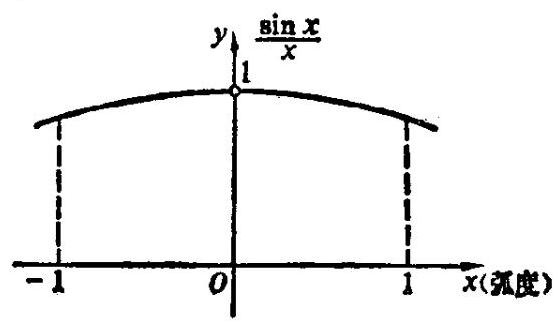
\includegraphics[max width=0.6\textwidth]{images/01912c18-5c3f-733d-b775-749ba9897a9d_42_483969.jpg}
\end{center}

图 1-9

\begin{center}
	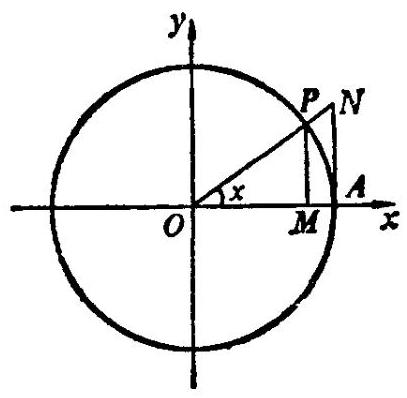
\includegraphics[max width=0.4\textwidth]{images/01912c18-5c3f-733d-b775-749ba9897a9d_42_838953.jpg}
\end{center}

图 1-10

从上表和图 1-9 可以看出,当 \(x\) 无限趋近于 0 时,函数 \(\frac{\sin x}{x}\) 的值无限趋近于 1,即 \(\mathop{\lim }\limits_{{x \rightarrow 0}}\frac{\sin x}{x} = 1\) . 下面我们利用上面的定理来证明这个结论.

如图 1-10,在单位圆中,以 \({OA}\) 为始边的圆心角 \(x\) (不大的正角) 是用弧度来度量的,角的终边与圆相交于 \(P.{MP} \bot\) \({OA},{AN}\) 是过圆 \(O\) 上 \(A\) 点的切线,它和 \({OP}\) 相交于 \(N\) . 从图中知道,

\[
{MP} = \sin x,\overset{⏜}{PA} = x,{AN} = \operatorname{tg}x,
\]

那么面积

\[
{S}_{\bigtriangleup {OAP}} = \frac{1}{2}\sin x,{S}_{\text{焦形 }{OAP}} = \frac{1}{2}x,
\]

\[
{S}_{\bigtriangleup {OAN}} = \frac{1}{2}\operatorname{tg}x.
\]

由

\[
{S}_{\bigtriangleup {OAP}} < {S}_{\text{底形 }{OAP}} < {S}_{\bigtriangleup {OAN}},
\]

得

\[
\sin x < x < \operatorname{tg}x\text{.}
\]

当自变量 \(x\) 取正值趋近于 0 时, \(\sin x > 0\) ,因此,

\[
1 < \frac{x}{\sin x} < \frac{\operatorname{tg}x}{\sin x}
\]

即

\[
1 < \frac{x}{\sin x} < \frac{1}{\cos x}
\]

于是,

\[
\cos x < \frac{\sin x}{x} < 1\text{.}
\]

因为余弦函数是连续函数,所以 \(\mathop{\lim }\limits_{{x \rightarrow 0 + }}\cos x = 1\) . 根据上面判定函数极限存在的定理,得到当 \(x\) 取正值趋近于 0 时,

\[
\mathop{\lim }\limits_{{x \rightarrow 0 + }}\frac{\sin x}{x} = 1
\]

又当 \(x\) 取负值趋近于 0 时, \(- x \rightarrow 0, - x > 0,\sin \left( {-x}\right)\) \(> 0\) ,于是

\[
\mathop{\lim }\limits_{{x \rightarrow 0 - }}\frac{\sin x}{x} = \mathop{\lim }\limits_{{-x \rightarrow 0 + }}\frac{\sin \left( {-x}\right) }{-x} = 1.
\]

根据 1.3 节最后的定理, 由于

\[
\mathop{\lim }\limits_{{x \rightarrow 0 + }}\frac{\sin x}{x} = \mathop{\lim }\limits_{{x \rightarrow 0 - }}\frac{\sin x}{x} = 1
\]

所以有

\[
\mathop{\lim }\limits_{{x \rightarrow 0}}\frac{\sin x}{x} = 1
\]

在推导这个重要极限时,用到 \({S}_{\text{扇形 }{OAP}} = \frac{1}{2}x,x\) 以弧度为单位. 一般地, 在微积分中三角函数的自变量都是实数, 它对应于以弧度为单位的角或弧.

例 1 求 \(\mathop{\lim }\limits_{{x \rightarrow 0}}\frac{\operatorname{tg}x}{x}\) .

解: \(\mathop{\lim }\limits_{{x \rightarrow 0}}\frac{\operatorname{tg}x}{x} = \mathop{\lim }\limits_{{x \rightarrow 0}}\left( {\frac{\sin x}{x} \cdot \frac{1}{\cos x}}\right)\)

\[
= \mathop{\lim }\limits_{{x \rightarrow 0}}\frac{\sin x}{x} \cdot \mathop{\lim }\limits_{{x \rightarrow 0}}\frac{1}{\cos x}
\]

\[
= 1 \times 1 = 1\text{.}
\]

例 2 求 \(\mathop{\lim }\limits_{{x \rightarrow 0}}\frac{1 - \cos x}{{x}^{2}}\) .

解: \(\mathop{\lim }\limits_{{x \rightarrow 0}}\frac{1 - \cos x}{{x}^{2}} = \mathop{\lim }\limits_{{x \rightarrow 0}}\frac{2{\sin }^{2}\frac{x}{2}}{{x}^{2}}\)

\[
= \frac{1}{2}\mathop{\lim }\limits_{{x \rightarrow 0}}\frac{{\sin }^{2}\frac{x}{2}}{{\left( \frac{x}{2}\right) }^{2}}
\]

\(= \frac{1}{2}\mathop{\lim }\limits_{{\frac{x}{2} \rightarrow 0}}{\left( \frac{\sin \frac{x}{2}}{\frac{x}{2}}\right) }^{2}\left( {\text{ 当 }x \rightarrow 0\text{ 时,}\;\frac{x}{2} \rightarrow 0}\right)\)

\[
= \frac{1}{2}\mathop{\lim }\limits_{{\frac{x}{2} \rightarrow 0}}\left( \frac{\sin \frac{x}{2}}{\frac{x}{2}}\right) \cdot \mathop{\lim }\limits_{{\frac{x}{2} \rightarrow 0}}\left( \frac{\sin \frac{x}{2}}{\frac{x}{2}}\right) = \frac{1}{2} \times 1 \times 1 = \frac{1}{2}\text{.}
\]

\subsection*{2. \(\mathop{\lim }\limits_{{x \rightarrow \infty }}{\left( 1 + \frac{1}{x}\right) }^{x} = e\)}

我们从下表可以看出当 \(x \rightarrow + \infty\) 时函数 \({\left( 1 + \frac{1}{x}\right) }^{x}\) 的变化趋势:

\begin{center}
	\adjustbox{max width=\textwidth}{
		\begin{tabular}{|c|c|c|}
			\hline
			\(x\) & \({\left( 1 + \frac{1}{x}\right) }^{x}\) & 近 似 值 \\
			\hline
			1 & \({\left( 1 + \frac{1}{1}\right) }^{1}\) & 2 \\
			\hline
			10 & \({\left( 1 + \frac{1}{10}\right) }^{10}\) & 2. 59374 \\
			\hline
			100 & \({\left( 1 + \frac{1}{100}\right) }^{100}\) & 2. 70481 \\
			\hline
			1000 & \({\left( 1 + \frac{1}{1000}\right) }^{1000}\) & 2. 71692 \\
			\hline
			10000 & \({\left( 1 + \frac{1}{10000}\right) }^{10000}\) & 2. 71815 \\
			\hline
			100000 & \({\left( 1 + \frac{1}{100000}\right) }^{100000}\) & 2. 71827 \\
			\hline
			\(\cdots\) & \(\cdots\) & \(\cdots\) \\
			\hline
		\end{tabular}
	}
\end{center}

同样,当 \(x \rightarrow - \infty\) 时,函数 \({\left( 1 + \frac{1}{x}\right) }^{x}\) 有相同的变化趋势 (见下页的表).

可以证明,当 \(x\) 趋向无穷时, \({\left( 1 + \frac{1}{x}\right) }^{x}\) 趋近于无理数 \({2.71828182845}\cdots\) ,记作 \(e\) . 即

\[
\mathop{\lim }\limits_{{x \rightarrow \infty }}{\left( 1 + \frac{1}{x}\right) }^{x} = e
\]

\begin{center}
	\adjustbox{max width=\textwidth}{
		\begin{tabular}{|c|c|c|}
			\hline
			\(- 2\) & \({\left( 1 + \frac{1}{-2}\right) }^{-2}\) & 4 \\
			\hline
			\(- {10}\) & \({\left( 1 + \frac{1}{-{10}}\right) }^{-{10}}\) & 2. 86797 \\
			\hline
			\(- {100}\) & \({\left( 1 + \frac{1}{-{100}}\right) }^{-{100}}\) & 2. 73199 \\
			\hline
			\(- {1000}\) & \({\left( 1 + \frac{1}{-{1000}}\right) }^{-{1000}}\) & 2. 71964 \\
			\hline
			\(- {10000}\) & \({\left( 1 + \frac{1}{-{10000}}\right) }^{-{10000}}\) & 2. 71842 \\
			\hline
			\(- {100000}\) & \({\left( 1 + \frac{1}{-{100000}}\right) }^{-{100000}}\) & 2. 71830 \\
			\hline
			\(\cdots\) & \(\cdots\) & \(\cdots\) \\
			\hline
		\end{tabular}
	}
\end{center}

如果作一个变换 \(y = \frac{1}{x}\) ,那么当 \(x \rightarrow \infty\) 时, \(y \rightarrow 0\) ,于是又得到

\[
\mathop{\lim }\limits_{{y \rightarrow 0}}{\left( 1 + y\right) }^{\frac{1}{y}} = e
\]

无理数 \(e\) 是自然对数的底,它在微积分和其他科学技术中经常用到.

例 3 求 \(\mathop{\lim }\limits_{{x \rightarrow \infty }}{\left( 1 + \frac{1}{x}\right) }^{-x}\) .

解: \(\mathop{\lim }\limits_{{x \rightarrow \infty }}{\left( 1 + \frac{1}{x}\right) }^{-x} = \mathop{\lim }\limits_{{x \rightarrow \infty }}\frac{1}{{\left( 1 + \frac{1}{x}\right) }^{x}}\)

\[
= \frac{1}{\mathop{\lim }\limits_{{x \rightarrow \infty }}{\left( 1 + \frac{1}{x}\right) }^{x}} = \frac{1}{e}
\]

\begin{problemset}[练习]

\item 求下列极限:

(1) \(\mathop{\lim }\limits_{{x \rightarrow 0}}\frac{x}{\sin x}\) 

(2) \(\mathop{\lim }\limits_{{x \rightarrow 0}}\frac{\sin {4x}}{3x}\) .

\item 求下列极限:

(1) \(\mathop{\lim }\limits_{{x \rightarrow \infty }}{\left( 1 + \frac{1}{x}\right) }^{2x}\)

(2) \(\mathop{\lim }\limits_{{x \rightarrow 0}}{\left( 1 + x\right) }^{-\frac{1}{x}}\) .
\end{problemset}

\begin{problemset}[习 题 三]


\item 根据函数连续性的定义, 说明下列函数在给定点处连续:

(1) \(f\left( x\right) = {3x} + 1,x = \frac{1}{2}\) ;

(2) \(f\left( x\right) = a{x}^{2} + b,x = 1\) ;

(3) \(f\left( x\right) = \frac{4{x}^{2} - 1}{{2x} - 1},x = 2\) ;

(4) \(f\left( x\right) = a{x}^{3} + b{x}^{2} + {cx} + d,x = 0\) .

\item 说出下列函数在实数轴上哪些点处不连续:

(1) \(y = \frac{1}{{x}^{2} + {3x} + 2}\) (2) \(y = \frac{1}{\sin x}\) .

\item 写出由下列各组函数复合而成的复合函数:

(1) \(y = {u}^{2},u = \sin x\) ;

(2) \(y = \sin u,u = {x}^{2}\) ;

(3) \(y = {u}^{3},u = {x}^{2} + 1\) ;

(4) \(y = \ln \dot{u};u = {v}^{2} + 1,v = \sin x\) ;

(5) \(y = {e}^{u},u = {v}^{2},v = \operatorname{ctg}x\) ;

(6) \(y = \arcsin u,u = \sqrt{v},v = \frac{x - a}{b - a}\) .

\item 下列函数是由哪几个简单函数复合而成的?

(1) \(y = {\left( 1 + x\right) }^{5}\) ; (2) \(y = \frac{1}{{\left( 1 - {x}^{2}\right) }^{3}}\) ;

(3) \(y = \ln {\sin }^{2}{3x}\) ; (4) \(y = {e}^{2{\cos }^{2}x}\) ;

(5) \(y = \frac{1}{\sqrt{1 - \operatorname{tg}{3x}}}\) ; (6) \(y = {\left( 1 + \operatorname{arctg}{x}^{2}\right) }^{8}\) .

\item 求下列极限:

(1) \(\mathop{\lim }\limits_{{x \rightarrow 1}}\sqrt{{x}^{2} + {3x} - 2}\) ; (2) \(\mathop{\lim }\limits_{{u \rightarrow 1}}\frac{{u}^{2} + u + 2}{3 - u}\) ;

(3) \(\mathop{\lim }\limits_{{x \rightarrow {16}}}\frac{\sqrt[4]{x} - 2}{\sqrt{x} - 4}\) (4) \(\mathop{\lim }\limits_{{x \rightarrow 2}}\frac{\sqrt{{2x} - 2} - \sqrt{x}}{{x}^{2} - 4}\) ;

(5) \(\mathop{\lim }\limits_{{\alpha \rightarrow \frac{\pi }{4}}}{\left( 1 + \sin 2\alpha \right) }^{2}\) ; (6) \(\mathop{\lim }\limits_{{x \rightarrow 2}}{\log }_{3}\left( {{x}^{3} + 1}\right)\) .

\item 求下列极限:

(1) \(\mathop{\lim }\limits_{{x \rightarrow 0}}\frac{x}{\operatorname{tg}{3x}}\) (2) \(\mathop{\lim }\limits_{{x \rightarrow 0}}\frac{\sin {3x}}{\sin {5x}}\)

(3) \(\mathop{\lim }\limits_{{x \rightarrow 0}}\frac{\sin x\operatorname{tg}x}{{x}^{2}}\) (4) \(\mathop{\lim }\limits_{{x \rightarrow 0}}\frac{1 - \cos {2x}}{x\sin x}\) .

\item 求下列极限:

(1) \(\mathop{\lim }\limits_{{x \rightarrow \infty }}{\left( 1 + \frac{1}{x}\right) }^{x + 2}\) (2) \(\mathop{\lim }\limits_{{x \rightarrow \infty }}{\left( 1 + \frac{2}{x}\right) }^{\frac{x}{2}}\)

(3) \(\mathop{\lim }\limits_{{x \rightarrow 0}}{\left( 1 + 2x\right) }^{\frac{1}{x}}\) (4) \(\mathop{\lim }\limits_{{x \rightarrow \infty }}{\left( 1 - \frac{1}{x}\right) }^{2x}\) .
\end{problemset}

\chapter*{小 结}
\markboth{小 结}{小 结}

一、本章的主要内容是数列的极限的概念及其运算法则; 函数的极限的概念及其运算法则; 函数连续的概念和初等函数的连续性; 两个重要的极限, 即

\[
\mathop{\lim }\limits_{{x \rightarrow 0}}\frac{\sin x}{x} = 1,\;\mathop{\lim }\limits_{{x \rightarrow \infty }}{\left( 1 + \frac{1}{x}\right) }^{x} = e.
\]

二、极限是描述数列和函数在无限过程中的变化趋势的重要概念. 极限方法是人们从有限中认识无限, 从近似中认识精确, 从量变中认识质变的一种数学方法, 它是微积分的基本思想和方法.

数列的极限与函数的极限的运算法则是类似的: 两个数列 (或函数) 的和、差、积、商的极限分别等于这两个数列 (或函数) 的极限的和、差、积、商 (作为除数的数列或函数的极限不能为零). 运用这些运算法则, 可以简化极限的计算过程.

三、连续的概念是用极限的概念定义的, 但是连续和极限是有区别的: 极限所讨论的是函数在某一点附近的变化趋势, 而不管函数在这一点上是否有定义或取什么值; 函数在一点处连续不仅要求在这一点有极限, 而且要求极限同这一点的函数值相等.

四、幂函数、指数函数、对数函数、三角函数和反三角函数, 统称基本初等函数.

由基本初等函数和常数经过有限次四则运算和有限次函数的复合而得出的函数, 统称初等函数.

基本初等函数和一切初等函数在它们的定义区间上是连续函数。

\chapter*{复习参考题一}
\markboth{复习参考题一}{复习参考题一}
\section*{\(A\) 组}

1. 求无穷等比数列 \(\left\{ {q}^{n}\right\}\) 当 \(q = \frac{1}{2}\) 时前 10 项的和与前 100 项的和。

2. 作图表示下列无穷数列, 并说出数列是否趋近于某一常数:

(1) \(\left\{ {1 + {\left( -1\right) }^{n}\frac{2}{n}}\right\}\) (2) \(\left\{ \frac{{\left( n - 1\right) }^{2}}{2n}\right\}\)

(3) \(\left\{ {\left( -\frac{1}{n}\right) }^{3}\right\}\) (4) \(\{ \sqrt{n}\}\) .

3. 已知数列 \(\left\{ \frac{1}{{3}^{n}}\right\}\) ,根据下表中给出的 \(\varepsilon\) 的数值,求出相应的正整数 \(N\) ,使得当 \(n > N\) 时, \(\left| {\frac{1}{{3}^{n}} - 0}\right| < \varepsilon\) 恒成立.

\begin{center}
	\adjustbox{max width=\textwidth}{
		\begin{tabular}{|c|c|c|c|c|}
			\hline
			e & 0.1 & 0.02 & 0.003 & 0.0001 \\
			\hline
			\(N\) & \phantom{X} & \phantom{X} & \phantom{X} & \phantom{X} \\
			\hline
		\end{tabular}
	}
\end{center}

4. 举出两个极限是 7 的无穷数列.

5. 举出两个没有极限的无穷数列。

6. 求下列数列的极限:

(1) \(\mathop{\lim }\limits_{{n \rightarrow \infty }}\frac{{2n} + 1}{n}\) (2) \(\mathop{\lim }\limits_{{n \rightarrow \infty }}\frac{3n}{n + 1}\)

(3) \(\mathop{\lim }\limits_{{n \rightarrow \infty }}\frac{{n}^{2}}{{n}^{2} - n}\) (4) \(\mathop{\lim }\limits_{{n \rightarrow \infty }}\frac{1}{{n}^{2} + 1}\) .

7. (1) 求 \(\mathop{\lim }\limits_{{n \rightarrow \infty }}\frac{1 + 2 + 3 + \cdots + n}{1 + 3 + 5 + \cdots + \left( {{2n} - 1}\right) }\) ;

(2)求 \(\mathop{\lim }\limits_{{n \rightarrow \infty }}\frac{1 + \frac{1}{2} + \frac{1}{4} + \cdots + \frac{1}{{2}^{n}}}{1 + \frac{1}{3} + \frac{1}{9} + \cdots + \frac{1}{{3}^{n}}}\) .

8. 求下列极限:

(1) \(\mathop{\lim }\limits_{{n \rightarrow \infty }}\left( {\frac{1}{n} + \frac{{2n} - 1}{3n}}\right)\) ; (2) \(\mathop{\lim }\limits_{{n \rightarrow \infty }}\frac{5{n}^{2} + 7}{3{n}^{2} + n - 1}\)

(3) \(\mathop{\lim }\limits_{{n \rightarrow \infty }}\frac{\left( {n - 1}\right) \left( {n + 1}\right) \left( {n + 2}\right) }{2{n}^{3}}\) ; (4) \(\mathop{\lim }\limits_{{n \rightarrow \infty }}\frac{{\left( n - 1\right) }^{3}}{{n}^{3} + 1}\) ;

(5) \(\mathop{\lim }\limits_{{x \rightarrow 1}}\left( {\frac{1}{1 - x} - \frac{3}{1 - {x}^{3}}}\right)\) ;

(6) \(\mathop{\lim }\limits_{{x \rightarrow \infty }}\left( {\frac{{x}^{3}}{2{x}^{2} - 1} - \frac{{x}^{2}}{{2x} + 1}}\right)\) .

9. 已知 \(f\left( x\right) = \frac{{a}_{0}{x}^{m} + {a}_{1}{x}^{m - 1} + \cdots + {a}_{m}}{{b}_{0}{x}^{m} + {b}_{1}{x}^{n - 1} + \cdots + {b}_{n}}\) ,而且 \({x}_{0}\) 不是 \(f\left( x\right)\) 的分母的根:

(1)求 \(\mathop{\lim }\limits_{{x \rightarrow {x}_{0}}}f\left( x\right)\) ;

(2)当 \(m \leq n\) 时,求 \(\mathop{\lim }\limits_{{x \rightarrow \infty }}f\left( x\right)\) .

10. 说出下列函数是怎样复合而成的:

(1) \(y = {\left( a + bx\right) }^{5}\) ; (2) \(y = {\left( \arccos \sqrt{1 - {x}^{2}}\right) }^{3}\) ;

(3) \(y = \operatorname{arctg}\sqrt[5]{{x}^{3} - 1}\) ; (4) \(y = {e}^{\frac{1}{2}\lg \left( {{ax} + b}\right) }\) .

11. 求下列极限:

(1) \(\mathop{\lim }\limits_{{x \rightarrow \sqrt{2}}}\frac{2{x}^{2} - 1}{{x}^{4} + 2{x}^{2} - 1}\) (2) \(\mathop{\lim }\limits_{{a \rightarrow \frac{\pi }{3}}}\left( {\sin {2\theta } + \cos {2\theta }}\right)\) ;

(3) \(\mathop{\lim }\limits_{{x \rightarrow a}}\frac{\sin x - \sin a}{x - a}\) ; (4) \(\mathop{\lim }\limits_{{x \rightarrow 0}}\frac{{\sin }^{2}{3x}}{x\sin {2x}}\)

(5) \(\mathop{\lim }\limits_{{x \rightarrow 2}}\frac{x - 2}{\sqrt{x - 1} - 1}\) ; (6) \(\mathop{\lim }\limits_{{x \rightarrow 3}}\frac{\sqrt{1 + x} - 2}{x - 3}\) .

12. 求下列极限:

(1) \(\mathop{\lim }\limits_{{x \rightarrow 0}}\frac{{x}^{2}}{{\sin }^{2}\left( \frac{x}{3}\right) }\) (2) \(\mathop{\lim }\limits_{{x \rightarrow 0}}\left( {x \cdot \operatorname{ctg}x}\right)\) ;

(3) \(\mathop{\lim }\limits_{{x \rightarrow \infty }}{\left( \frac{x}{1 + x}\right) }^{x}\) ; (4) \(\mathop{\lim }\limits_{{x \rightarrow \infty }}{\left( 1 + \frac{2}{x}\right) }^{x}\) .

\section*{B 组}

13. 下面的数列中, 哪些有极限? 如果数列有极限, 说出它的极限。

(1) \(1,{0.1},{0.01},{0.001},\cdots \cdots\) ;

(2) \(+ 2, - 2, + 2, - 2,\cdots \cdots\) ;

(3) \(\left\{ \frac{\sqrt{n} + 1}{n}\right\}\)

(4) \(\left\{ {q}^{n}\right\}\) (提示: 分 \(q = 1,q = - 1;\left| q\right| < 1,\left| q\right| > 1\) 四种情况讨论).

14. 已知 \(a > 0\) ,求下列极限:

(1) \(\mathop{\lim }\limits_{{n \rightarrow \infty }}\frac{1}{1 + {a}^{n}}\) (2) \(\mathop{\lim }\limits_{{n \rightarrow \infty }}\frac{{a}^{n}}{1 + {a}^{n}}\) .

15. 如图,从 \(\angle {BAC}\) 的边上一点 \(B\) 作 \({BC} \bot {AC}\) ,从 \(C\) 作 \({CD} \bot\) \({AB}\) ,从 \(D\) 再作 \({DE} \bot {AC}\) ,这样无限进行下去. 假定 \({BC} =\) \(7\mathrm{\;{cm}},{CD} = 6\mathrm{\;{cm}}\) ,求这些垂线长的和.

\begin{center}
	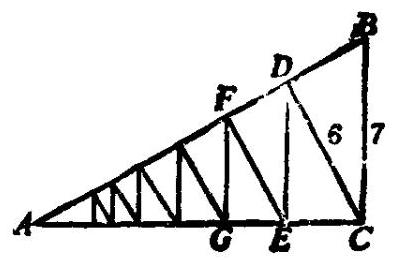
\includegraphics[max width=0.4\textwidth]{images/01912c18-5c3f-733d-b775-749ba9897a9d_52_461588.jpg}
\end{center}

(第 15 题)

16. 将下列循环小数化成分数:

(1) \({0.2}\dot{7}\) ; (2) 2.5142857 .

17. 求下列极限:

(1) \(\mathop{\lim }\limits_{{x \rightarrow \infty }}\frac{{x}^{2} + 2}{{x}^{2} + x + 1}\)

(2) \(\mathop{\lim }\limits_{{x \rightarrow \infty }}\frac{{x}^{2} + 1}{4{x}^{3} - 1}\)

(3) \(\mathop{\lim }\limits_{{x \rightarrow - \infty }}\frac{3{x}^{2} - 1}{{x}^{2} + {2x}}\)

(4) \(\mathop{\lim }\limits_{{x \rightarrow + \infty }}\frac{5{x}^{2} + x - 3}{4{x}^{2} - {2x} + 1}\) .

18. 求下列极限:

(1) \(\mathop{\lim }\limits_{{x \rightarrow 3}}\frac{{x}^{2} - 9}{{x}^{2} - {4x} + 3}\) (2) \(\mathop{\lim }\limits_{{u \rightarrow 1}}\frac{{u}^{3} - 1}{{u}^{2} - 1}\)

(3) \(\mathop{\lim }\limits_{{x \rightarrow 1}}\frac{{x}^{m} - 1}{{x}^{n} - 1}\;\left( {m,n\text{是自然数}}\right)\) .

19. 求下列无穷数列各项的和 \(S\) :

(1) \(\frac{1}{1 \cdot 2},\frac{1}{2 \cdot 3},\cdots ,\frac{1}{n\left( {n + 1}\right) },\cdots\)

\[
\text{提示:}\left. {\frac{1}{n\left( {n + 1}\right) } = \frac{1}{n} - \frac{1}{n + 1}}\right\rbrack \text{;}
\]

(2) \(\frac{2}{{2}^{2} - 1},\frac{2}{{3}^{2} - 1},\cdots ,\frac{2}{{\left( n + 1\right) }^{2} - 1},\cdots\)

\[
\left\lbrack {\text{提示:}\frac{1}{{\left( n + 1\right) }^{2} - 1} = \frac{1}{n\left( {n + 2}\right) }}\right\rbrack \text{.}
\]

20. 求下列极限:

(1) \(\mathop{\lim }\limits_{{x \rightarrow 1}}\frac{\sqrt[3]{x} - 1}{\sqrt{x} - 1}\)

(2) \(\mathop{\lim }\limits_{{x \rightarrow \infty }}\left( {\sqrt{{x}^{2} + 1} - \sqrt{{x}^{2} - 1}}\right)\) .

21. 求下列极限:

(1) \(\mathop{\lim }\limits_{{x \rightarrow \infty }}{\left( 1 + \frac{3}{x}\right) }^{x}\) ; (2) \(\mathop{\lim }\limits_{{x \rightarrow 0}}{\left( 1 + x\right) }^{\frac{1}{x} + 2}\) ;

(3) \(\mathop{\lim }\limits_{{x \rightarrow 0}}{\left( 1 + \operatorname{tg}x\right) }^{\operatorname{ctg}x}\) ; (4) \(\mathop{\lim }\limits_{{x \rightarrow 1}}\frac{\sin \left( {1 - x}\right) }{1 - {x}^{2}}\) .

\chapter{导数和微分}

\section*{导 数 概 念}

\section{瞬时速度}

我们知道,物体作匀速直线运动时,物体的位移 \(s\) 与所经过的时间 \(t\) 的比,就是物体运动的速度 \(v\) ,即

\[
v = \frac{s}{t}
\]

这个速度在匀速直线运动过程中的任何时刻都是一样的.

如果物体作非匀速直线运动, 也就是说, 在运动过程的各个时刻, 物体运动的快慢不一样, 这时, 设已知物体的运动规律是 \(s = s\left( t\right)\) ,从 \({t}_{0}\) 到 \({t}_{0} + {\Delta t}({\Delta t}\) 称为时间改变量) 这段时间内, 物体的位移 (即位置改变量) 是

\[
{\Delta s} = s\left( {{t}_{0} + {\Delta t}}\right) - s\left( {t}_{0}\right) ,
\]

那么,位置改变量 \({\Delta s}\) 与时间改变量 \({\Delta t}\) 的比,就是这段时间内物体的平均速度 \(\bar{v}\) ,即

\[
\bar{v} = \frac{\Delta s}{\Delta t} = \frac{s\left( {{t}_{0} + {\Delta t}}\right) - s\left( {t}_{0}\right) }{\Delta t}.
\]

平均速度的大小反映在这段时间内物体运动快慢的平均程度.

为了更精确地刻划非匀速运动, 还需知道物体在某一时刻的“速度”. 那么, 作非匀速直线运动的物体在某一时刻的 “速度”怎样求呢?

现在我们以自由落体运动为例, 来说明作非匀速直线运动的物体在某一时刻的“速度”的求法.

我们知道, 自由落体运动的方程是

\[
s = s\left( t\right) = \frac{1}{2}g{t}^{2},
\]

这里 \(g\) 是重力加速度,通常取 \(g = {9.8}\) 米 \(/{\text{秒}}^{2}\) . 现在来求 \(t = 3\) 秒这一时刻落体的 “速度”.

当 \({\Delta t}\) 很小时,从 3 秒到 \(3 + {\Delta t}\) 秒这段时间内,落体运动的快慢变化也不大, 因此, 可以用这段时间内的平均速度近似地反映落体在 3 秒时的 “速度”. 当 \({\Delta t}\) 越小时,一般来讲,这种近似就越精确. 现在我们来计算一下 \(t\) 从 3 秒 分别到 3.1 秒、 3.01 秒、 3.001 秒、 3.0001 秒、……, 各段时间内的平均速度, 把所得数据列表如下:

\begin{center}
\adjustbox{max width=\textwidth}{
\begin{tabular}{|c|c|c|c|c|}
\hline
\(t\left( \text{ 秒 }\right)\) & 8 (米) & \({\Delta t}\) (秒) & \({\Delta s}\) (米) & \(\bar{v} = \frac{\Delta s}{\Delta t}\left( {\text{ 米 }/\text{ 秒 }}\right)\) \\
\hline
3 & 4. \(5\mathrm{\;g}\) & \phantom{X} & \phantom{X} & \phantom{X} \\
\hline
3. 1 & \({4.805g}\) & 0.1 & \({0.305g}\) & \({3.05g}\) \\
\hline
3.01 & 4. \({53005g}\) & 0.01 & 0.03005g & 3. \({005}\mathrm{\;g}\) \\
\hline
3.001 & 4. 5030005g & 0.001 & 0.0030005g & 3.00059 \\
\hline
3.0001 & 4.500300005g & 0.0001 & 0.000300005g & 3.00005g \\
\hline
\(\cdots\) & ... & . & ... & ... \\
\hline
\end{tabular}
}
\end{center}

从上表可以看出,平均速度 \(\frac{\Delta s}{\Delta t}\) 随着 \({\Delta t}\) 变化而变化,当

\({\Delta t}\) 越小时, \(\frac{\Delta s}{\Delta t}\) 越接近于一个定值一 \({3g}\) . 这个值就是 \({\Delta t} \rightarrow 0\) 时 \(\frac{\Delta s}{\Delta t}\) 的极限. 我们规定这个极限为落体在 \(t = 3\) 秒时的速度,也叫瞬时速度,用 \(v\) 表示. 根据第一章求极限的法则,得

\[
v = \mathop{\lim }\limits_{{{\Delta t} \rightarrow 0}}\frac{s\left( {3 + {\Delta t}}\right) - s\left( 3\right) }{\Delta t}
\]

\[
= \mathop{\lim }\limits_{{{\Delta t} \rightarrow 0}}\frac{\frac{1}{2}g{\left( 3 + \Delta t\right) }^{2} - \frac{1}{2}g \cdot {3}^{2}}{\Delta t}
\]

\[
= \frac{g}{2}\mathop{\lim }\limits_{{{\Delta t} \rightarrow 0}}\left( {6 + {\Delta t}}\right)
\]

\[
= {3g} = {29.4}\text{ (米/秒). }
\]

一般地,我们规定,非匀速直线运动在某一时刻 \({t}_{0}\) 的瞬时速度 \(v\) ,就是运动物体在 \({t}_{0}\) 到 \({t}_{0} + {\Delta t}\) 一段时间内的平均速度当 \({\Delta t} \rightarrow 0\) 时的极限,即

\[
v = \mathop{\lim }\limits_{{{\Delta t} \rightarrow 0}}\frac{\Delta s}{\Delta t} = \mathop{\lim }\limits_{{{\Delta t} \rightarrow 0}}\frac{s\left( {{t}_{0} + {\Delta t}}\right) - s\left( {t}_{0}\right) }{\Delta t}.
\]

平均速度 \(\frac{\Delta s}{\Delta t}\) 在 \({\Delta t} \rightarrow 0\) 时转化为瞬时速度,瞬时速度的大小刻划了物体在某一时刻运动的快慢.

\begin{problemset}[练习]

\item 一球沿某一斜面自由滚下,测得滚下的垂直距离 \(y\) 与时间 \(x\) 之间的函数关系为 \(y = {x}^{2}\) .

(1)求时间 \(x\) 从 5 秒分别到 6 秒、5.1 秒、5.01 秒、5.001 秒、 \(5 + h\) 秒的时间改变量 \({\Delta x}\) ,对应的垂直距离改变

量 \({\Delta y}\) 以及这段时间内垂直方向的平均速 度 \(\frac{\Delta y}{\Delta x}\) ,并填下表:

\begin{center}
\adjustbox{max width=\textwidth}{
\begin{tabular}{|c|c|c|c|}
\hline
\phantom{X} & \({\Delta x}\) (秒) & \({\Delta y}\left( \text{ 米 }\right)\) & \(\frac{\Delta y}{\Delta x}\left( {\text{米}/\text{秒}}\right)\) \\
\hline
从 5 秒到 6 秒 从 5 秒到 5.1 秒 & \phantom{X} & \phantom{X} & \phantom{X} \\
\hline
从 5 秒到 5.01 秒 & \phantom{X} & \phantom{X} & \phantom{X} \\
\hline
从 5 秒到 5.001 秒 & \phantom{X} & \phantom{X} & \phantom{X} \\
\hline
从 5 秒到 \(5 + h\) 秒 & \phantom{X} & \phantom{X} & \phantom{X} \\
\hline
\end{tabular}
}
\end{center}

(2)求在 5 秒时垂直方向的瞬时速度.

\item 质点 \(M\) 按规律 \(s = 2{t}^{2} + {3t}\) 作直线运动 \((s\) 的单位为厘米, \(t\) 的单位为秒).

(1)设 \({t}_{0},{\Delta t}\) 已给定,求相应的 \({\Delta s},\frac{\Delta s}{\Delta t}\) 和 \(\mathop{\lim }\limits_{{{\Delta t} \rightarrow 0}}\frac{\Delta s}{\Delta t}\) ,并说明它们的物理意义;

(2)求出质点 \(M\) 从 2 秒分别到 2.1 秒、2.01 秒、 2.001 秒、 \(2 + {\Delta t}\) 秒各段时间内的平均速度;

(3)求质点 \(M\) 在 \(t = 2\) 秒时的瞬时速度。
\end{problemset}

\section{导数}

从上节的讨论可以看出, 当物体作匀速直线运动时, 我们可以直接根据位移和时间的比值来求速度; 当物体的位移随着时间的改变可能是非均匀变化时, 要研究在某一时刻物体运动的快慢, 就需要引进瞬时速度, 也就是位移函数对时间的瞬时变化率 (简称变化率) 的概念. 在自然科学和工程技术中, 经常遇到非均匀变化的问题, 例如化学反应速度、物体温度变化速度、放射物质的蜕变速度、电流强度等等. 因此, 撇开具体实际意义, 一般地从数量关系上来研究函数的变化率, 将对很多实际问题的解决具有普遍意义. 为此, 我们引进一个新的数学概念一导数.

设函数 \(y = f\left( x\right)\) 在点 \(x = {x}_{0}\) 及其附近有定义. 当自变量 \(x\) 在 \({x}_{0}\) 处有改变量 \({\Delta x}\) ( \({\Delta x}\) 可正可负),则函数 \(y\) 相应地有改变量

\[
{\Delta y} = f\left( {{x}_{0} + {\Delta x}}\right) - f\left( {x}_{0}\right) .
\]

这两个改变量的比

\[
\frac{\Delta y}{\Delta x} = \frac{f\left( {{x}_{0} + {\Delta x}}\right) - f\left( {x}_{0}\right) }{\Delta x}
\]

叫做函数 \(y = f\left( x\right)\) 在 \({x}_{0}\) 到 \({x}_{0} + {\Delta x}\) 之间的平均变化率.

如果 当 \({\Delta x} \rightarrow 0\) 时, \(\frac{\Delta y}{\Delta x}\) 有极限,我们就说函数 \(y = f\left( x\right)\) 在点 \({x}_{0}\) 处可导,并把这一极限叫做 \(f\left( x\right)\) 在点 \({x}_{0}\) 处的导数 (或变化率),记作 \({f}^{\prime }\left( {x}_{0}\right)\) 或 \({\left. {y}^{\prime }\right| }_{x = {x}_{0}}\) ,即

\[
{f}^{\prime }\left( {x}_{0}\right) = \mathop{\lim }\limits_{{{\Delta x} \rightarrow 0}}\frac{\Delta y}{\Delta x} = \mathop{\lim }\limits_{{{\Delta x} \rightarrow 0}}\frac{f\left( {{x}_{0} + {\Delta x}}\right) - f\left( {x}_{0}\right) }{\Delta x}. \tag{1}
\]

因此,函数 \(f\left( x\right)\) 在点 \({x}_{0}\) 处的导数就是函数的平均变化率当自变量的改变量趋向于零时的极限 \({f}^{\prime }\left( {x}_{0}\right)\) ,它反映了函数 \(f\left( x\right)\) 在点 \({x}_{0}\) 处变化的 “速度”.

如果上述极限不存在,我们就说函数 \(f\left( x\right)\) 在点 \({x}_{0}\) 处不可导或导数不存在.

根据导数的定义,瞬时速度就是位移函数 \(s\left( t\right)\) 对时间 \(t\)

的导数,自由落体在 \(t = 3\) 秒时的速度就是 \(s = \frac{1}{2}g{t}^{2}\) 在点 \(t =\) 3 处的导数. 即

\[
v = {\left. {s}^{\prime }\right| }_{t = 3} = \mathop{\lim }\limits_{{{\Delta t} \rightarrow 0}}\frac{\frac{1}{2}g{\left( 3 + \Delta t\right) }^{2} - \frac{1}{2}g \cdot {3}^{2}}{\Delta t}
\]

\[
= {3g} = {29.4}\text{ (米/秒). }
\]

由导数的定义,直接得出求函数 \(f\left( x\right)\) 在点 \({x}_{0}\) 处的导数的方法:

1. 求改变量 \({\Delta y} = f\left( {{x}_{0} + {\Delta x}}\right) - f\left( {x}_{0}\right)\) ;

2. 求比 \(\frac{\Delta y}{\Delta x} = \frac{f\left( {{x}_{0} + {\Delta x}}\right) - f\left( {x}_{0}\right) }{\Delta x}\) ;

3. 求极限 \(\mathop{\lim }\limits_{{{\Delta x} \rightarrow 0}}\frac{\Delta y}{\Delta x}\) .

例 1 求 \(y = {x}^{2}\) 在点 \(x = 1\) 处的导数.

解: \(\;{\Delta y} = {\left( 1 + \Delta x\right) }^{2} - {1}^{2} = {2\Delta x} + {\left( \Delta x\right) }^{2}\) ,

\[
\frac{\Delta y}{\Delta x} = \frac{{2\Delta x} + {\left( \Delta x\right) }^{2}}{\Delta x} = 2 + {\Delta x},
\]

\[
\mathop{\lim }\limits_{{{\Delta x} \rightarrow 0}}\frac{\Delta y}{\Delta x} = \mathop{\lim }\limits_{{{\Delta x} \rightarrow 0}}\left( {2 + {\Delta x}}\right) = 2
\]

\[
\therefore {\left. \;{y}^{\prime }\right| }_{x = 1} = 2\text{. }
\]

如果函数 \(f\left( x\right)\) 在开区间 \(\left( {a,b}\right)\) 内每一点处都可导,就说 \(f\left( x\right)\) 在开区间 \(\left( {a,b}\right)\) 内可导. 这时,对于开区间 \(\left( {a,b}\right)\) 内每一个确定的值 \({x}_{0}\) ,都对应着一个确定的导数 \({f}^{\prime }\left( {x}_{0}\right)\) ,这样就在开区间 \(\left( {a,b}\right)\) 内,构成一个新的函数,我们把这一新函数叫做 \(f\left( x\right)\) 的导函数,记为 \({f}^{\prime }\left( x\right)\) 或 \({y}^{\prime }\) (有必要指明自变量 \(x\) 时记作 \(\left. {y}_{x}^{\prime }\right)\) . 根据导数的定义,就可得出导函数

\[
{y}^{\prime } = {f}^{\prime }\left( x\right) = \mathop{\lim }\limits_{{{\Delta x} \rightarrow 0}}\frac{\Delta y}{\Delta x} = \mathop{\lim }\limits_{{{\Delta x} \rightarrow 0}}\frac{f\left( {x + {\Delta x}}\right) - f\left( x\right) }{\Delta x}. \tag{2}
\]

导函数也简称为导数. 今后, 如不特别指明求某一点处的导数,求导数就是指求导函数. 但要注意,函数 \(y = f\left( x\right)\) 的导函数 \({f}^{\prime }\left( x\right)\) 与函数 \(y = f\left( x\right)\) 在点 \({x}_{0}\) 处的导数是有区别的, \({f}^{\prime }\left( x\right)\) 是 \(x\) 的函数,而 \({f}^{\prime }\left( {x}_{0}\right)\) 是一个数值; 但它们又是有联系的, \(f\left( x\right)\) 在点 \({x}_{0}\) 处的导数 \({f}^{\prime }\left( {x}_{0}\right)\) 就是导函数 \({f}^{\prime }\left( x\right)\) 在点 \({x}_{0}\) 处的函数值.

这样,如果知道了导函数 \({f}^{\prime }\left( x\right)\) ,要求 \(f\left( x\right)\) 在点 \({x}_{0}\) 处的导数,只要把 \(x = {x}_{0}\) 代入 \({f}^{\prime }\left( x\right)\) 中去求函数值就可以了.

例 2 已知 \(y = {x}^{3} - {2x} + 1\) ,求 \({y}^{\prime }\) ,并求在点 \(x = 2\) 处的导数.

解: \({\Delta y} = {\left( x + \Delta x\right) }^{3} - 2\left( {x + {\Delta x}}\right) + 1 - \left( {{x}^{3} - {2x} + 1}\right)\)

\[
= \left( {3{x}^{2} - 2}\right) {\Delta x} + {3x}{\left( \Delta x\right) }^{2} + {\left( \Delta x\right) }^{3},
\]

\[
\frac{\Delta y}{\Delta x} = 3{x}^{2} - 2 + {3x\Delta x} + {\left( \Delta x\right) }^{2},
\]

\[
\therefore \;{y}^{\prime } = \mathop{\lim }\limits_{{{\Delta x} \rightarrow 0}}\frac{\Delta y}{\Delta x} = 3{x}^{2} - 2,
\]

\[
{\left. {y}^{\prime }\right| }_{x = 2} = 3 \times {2}^{2} - 2 = {10}.
\]

例 3 已知 \(y = \sqrt{x}\) ,求 \({y}^{\prime }\) .

解: \({\Delta y} = \sqrt{x + {\Delta x}} - \sqrt{x}\) ,

\[
\frac{\Delta y}{\Delta x} = \frac{\sqrt{x + {\Delta x}} - \sqrt{x}}{\Delta x}.
\]

\[
\therefore {y}^{\prime } = \mathop{\lim }\limits_{{{\Delta x} \rightarrow 0}}\frac{\Delta y}{\Delta x} = \mathop{\lim }\limits_{{\Delta \dot{x} \rightarrow 0}}\frac{\sqrt{x + {\Delta x}} - \sqrt{x}}{\Delta x}
\]

\[
= \mathop{\lim }\limits_{{{\Delta x} \rightarrow 0}}\frac{1}{\sqrt{x + {\Delta x}} + \sqrt{x}} = \frac{1}{2\sqrt{x}}
\]

\begin{problemset}[练习]

\item 求下列函数在指定点处的导数:

(1) \(y = {x}^{3}\) ,点 \(x = 0\) ; (2) \(y = \frac{2}{x}\) ,点 \(x = 1\) .

\item 已知一物体作直线运动,运动方程为 \(s = 4{t}^{2}\) (米),求:

(1) \(t\) 秒时的瞬时速度;

(2) \(t = 3\) 秒、 \(t = 5\) 秒、 \(t = 8\) 秒时的瞬时速度.

\item 已知 \(y = \sqrt{x + 4}\) ,求 \({y}^{\prime }\) ,并求在点 \(x = 5\) 处的导数.

\end{problemset}

\section{导数的几何意义 切线方程和法线方程}

如图 2-1,设曲线 \(C\) 是函数 \(y = f\left( x\right)\) 的图象. 在曲线 \(C\) 上取一点 \(P\left( {{x}_{0},{y}_{0}}\right)\) 及点 \(P\) 邻近的任一点 \(Q\left( {{x}_{0} + }\right.\) \(\left. {{\Delta x},{y}_{0} + {\Delta y}}\right)\) ,过 \(P,Q\) 作割线, 并作 \({MP} \bot {Ox},{NQ} \bot {Ox}\) , \({PR} \bot {NQ}\) . 又设割线 \({PQ}\) 的倾斜角为 \(\beta\) ,那么

\[
\frac{\Delta y}{\Delta x} = \operatorname{tg}{QPR} = \operatorname{tg}\beta .
\]

\begin{center}
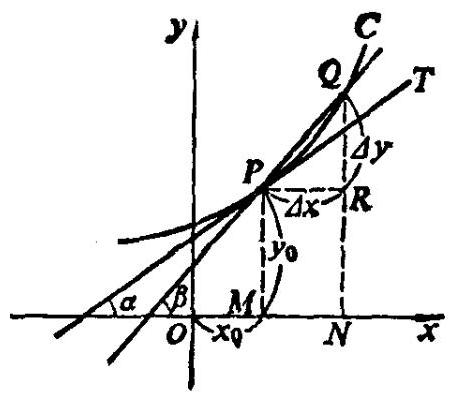
\includegraphics[max width=0.5\textwidth]{images/01912c18-5c3f-733d-b775-749ba9897a9d_62_329591.jpg}
\end{center}

图 2-1

这就是说, \(\frac{\Delta y}{\Delta x}\) 就是割线 \({PQ}\) 的斜率.

当点 \(Q\) 沿着曲线 \(O\) 无限地趋近于点 \(P\) ,即 \({\Delta x} \rightarrow 0\) 时,割线 \({PQ}\) 绕着点 \(P\) 转动,它的极限位置 \({PT}\) 叫做曲线 \(C\) 在点 \(P\) 处的切线. 这时如果函数 \(y = f\left( x\right)\) 在点 \({x}_{0}\) 处可导,那么当 \({\Delta x} \rightarrow 0\) 时, \(\frac{\Delta y}{\Delta x} \rightarrow {f}^{\prime }\left( {x}_{0}\right)\) ,而 \(\operatorname{tg}\beta\) 以 \({PT}\) 的斜率 \(\operatorname{tg}\alpha (\alpha\) 是 \({PT}\) 的倾斜角) 为极限, 所以

\[
{f}^{\prime }\left( {x}_{0}\right) = \operatorname{tg}\alpha \text{. }
\]

因此,函数 \(y = f\left( x\right)\) 在点 \({x}_{0}\) 处的导数 \({f}^{\prime }\left( {x}_{0}\right)\) 的几何意义,就是曲线 \(y = f\left( x\right)\) 在点 \(\left( {{x}_{0},f\left( {x}_{0}\right) }\right)\) 处的切线的斜率.

这样,求曲线 \(y = f\left( x\right)\) 在点 \(\left( {{x}_{0},f\left( {x}_{0}\right) }\right)\) 处的切线,只要先求出函数 \(y = f\left( x\right)\) 在点 \({x}_{0}\) 处的导数 \({f}^{\prime }\left( {x}_{0}\right)\) ,然后根据直线方程的点斜式, 就得到切线的方程

\[
y - {y}_{0} = {f}^{\prime }\left( {x}_{0}\right) \left( {x - {x}_{0}}\right)
\]

这里 \({y}_{0} = f\left( {x}_{0}\right)\) ,下同.

当 \(\alpha = \frac{\pi }{2}\) 时,导数不存在,这时切线 \({PT}\) 平行于 \(y\) 轴,切线的方程为

\[
x = {x}_{0}
\]

经过点 \(P\) 且和切线 \({PT}\) 垂直的直线叫做曲线 \(C\) 在点 \(P\) 处的法线. 由解析几何得知, 如果两条有斜率的直线互相垂直, 那么,它们的斜率互为负倒数. 已知曲线 \(y = f\left( x\right)\) 在点 \(\left( {x}_{0}\right.\) , \(\left. {f\left( {x}_{0}\right) }\right)\) 处的切线的斜率为 \({f}^{\prime }\left( {x}_{0}\right)\) ,那么,当 \({f}^{\prime }\left( {x}_{0}\right) \neq 0\) 时,曲线在该点处的法线的斜率为 \(- \frac{1}{{f}^{\prime }\left( {x}_{0}\right) }\) ,法线的方程为

\[
y - {y}_{0} = - \frac{1}{{f}^{\prime }\left( {x}_{0}\right) }\left( {x - {x}_{0}}\right) .
\]

当 \({f}^{\prime }\left( {x}_{0}\right) = 0\) 时,法线平行于 \(y\) 轴,法线的方程为

\[
x = {x}_{0}
\]

当切线 \({PT}\) 平行于 \(y\) 轴时,法线平行于 \(x\) 轴,这时法线的方程为

\[
y = {y}_{0}
\]

例 已知曲线 \(y = \frac{1}{3}{x}^{3}\) 上一点 \(P\left( {2,\frac{8}{3}}\right)\) . 求: (1) 过 \(P\) 点的切线的斜率; (2) 过 \(P\) 点的切线的方程; (3) 过 \(P\) 点的法线的方程.

解: (1) \(y = \frac{1}{3}{x}^{3}\) ,

\[
\therefore \;{y}^{\prime } = \mathop{\lim }\limits_{{{\Delta x} \rightarrow 0}}\frac{\Delta y}{\Delta x}
\]

\[
= \mathop{\lim }\limits_{{{\Delta x} \rightarrow 0}}\frac{\frac{1}{3}{\left( x + \Delta x\right) }^{3} - \frac{1}{3}{x}^{3}}{\Delta x}
\]

\[
= \frac{1}{3}\mathop{\lim }\limits_{{{\Delta x} \rightarrow 0}}\frac{3{x}^{2}{\Delta x} + {3x}{\left( \Delta x\right) }^{2} + {\left( \Delta x\right) }^{3}}{\Delta x}
\]

\[
= \frac{1}{3}\mathop{\lim }\limits_{{{\Delta x} \rightarrow 0}}\left\lbrack {3{x}^{2} + {3x\Delta x} + {\left( \Delta x\right) }^{2}}\right\rbrack
\]

\[
= {x}^{2}
\]

\[
{\left. {y}^{\prime }\right| }_{x = 2} = {2}^{2} = 4\text{. }
\]

\(\therefore\) 在点 \(P\) 处的切线的斜率等于 4 .

(2)在点 \(P\) 处的切线的方程为

\[
y - \frac{8}{3} = 4\left( {x - 2}\right)
\]

即

\[
{12x} - {3y} - {16} = 0.
\]

(3)在点 \(P\) 处的法线的方程为

\[
y - \frac{8}{3} = - \frac{1}{4}\left( {x - 2}\right)
\]

即

\[
{3x} + {12y} - {38} = 0\text{. }
\]

图形如图 2-2.

\begin{center}
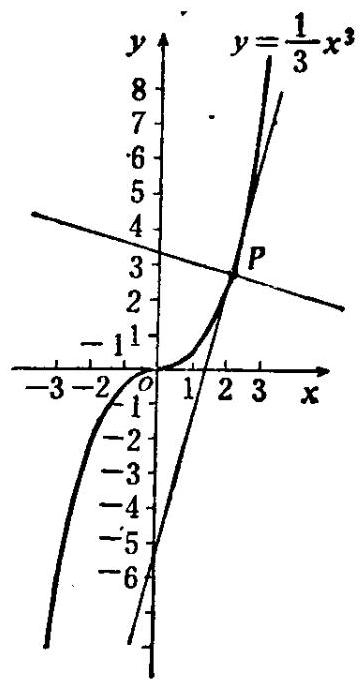
\includegraphics[max width=0.4\textwidth]{images/01912c18-5c3f-733d-b775-749ba9897a9d_65_242214.jpg}
\end{center}

图 2-2

\begin{problemset}[练习]

\item 求抛物线 \(y = {4x} - {x}^{2}\) 在点 \(A\left( {4,0}\right)\) 和点 \(B\left( {2,4}\right)\) 处的 \(\left( 1\right)\) 切线的斜率; (2) 切线的方程.

\item 求等边双曲线 \(y = \frac{9}{x}\) 在点 \(M\left( {3,3}\right)\) 处的切线的斜率与倾斜角。

\item 求抛物线 \(y = {x}^{2} + 2\) 在点 \(M\left( {2,6}\right)\) 处的切线方程和法线方程。

\end{problemset}

\section*{*变化率举例}

我们知道,函数 \(y = f\left( x\right)\) 的导数 \({f}^{\prime }\left( x\right)\) 就是函数对自变量 \(x\) 的变化率,因此,很多非均匀变化的变化率问题都可以应用导数来研究. 为了更好地理解和应用导数概念, 我们再举几个非均匀变化的变化率的例子.

例 1 瞬时功率.

已知物体所作的功 \(W\) 是时间 \(t\) 的函数: \(W = W\left( t\right)\) . 求在时刻 \(t = {t}_{0}\) 的功率.

分析: 功率表示作功的效率, 物体在某段时间内所作的功 \({\Delta W}\) 和这段时间 \({\Delta t}\) 的比 \(\frac{\Delta W}{\Delta t}\) ,就是这段时间内的(平均) 功率. 如果物体所作的功随时间增加而均匀改变, 这个比是个常数, 这个常数就是任一时刻的功率. 但是, 如果物体作功随时间的变化是非均匀的,那么, \(\frac{\Delta W}{\Delta t}\) 只表示某段时间内的平均功率. 因此,要求任一时刻 \({t}_{0}\) 的功率,就是求 \(\left\lbrack {{t}_{0},{t}_{0} + {\Delta t}}\right\rbrack\) 内的平均功率 \(\frac{\Delta W}{\Delta t}\) 当 \({\Delta t} \rightarrow 0\) 时的极限一瞬时功率.

解: 已知物体从 0 到 \(t\) 这段时间内所作的功是 \(W =\) \(W\left( t\right)\) ,那么,从时刻 \({t}_{0}\) 到 \({t}_{0} + {\Delta t}\) 这段时间内物体所作的功 (即功的改变量)为

\[
{\Delta W} = W\left( {{t}_{0} + {\Delta t}}\right) - W\left( {t}_{0}\right) .
\]

它和完成这些功所用时间(即时间改变量) \({\Delta t}\) 的比

\[
\frac{\Delta W}{\Delta t} = \frac{W\left( {{t}_{0} + {\Delta t}}\right) - W\left( {t}_{0}\right) }{\Delta t}
\]

就是 \({t}_{0}\) 到 \({t}_{0} + {\Delta t}\) 这段时间内的平均功率.

当 \({\Delta t} \rightarrow 0\) 时,平均功率的极限

\[
\mathop{\lim }\limits_{{{\Delta t} \rightarrow 0}}\frac{W\left( {{t}_{0} + {\Delta t}}\right) - W\left( {t}_{0}\right) }{\Delta t} = {P}_{0}
\]

就是在时刻 \({t}_{0}\) 的瞬时功率.

因此,功率 \(P\) 是功 \(W\) 对时间 \(t\) 的导数,即

\[
P = {W}^{\prime }\left( t\right)
\]

例 2 瞬时电流强度.

设有一随时间而变化的电流,从 0 到 \(t\) 这段时间内通过导线横截面的电量为 \(q = q\left( t\right)\) . 求在时刻 \({t}_{0}\) 时导线中的电流强度.

分析: 电流强度表示电流的强弱, 在某段时间内通过导线横截面的电量 \({\Delta q}\) 和这段时间 \({\Delta t}\) 的比 \(\frac{\Delta q}{\Delta t}\) ,就是这段时间内的电流强度. 如果给出的电流是稳恒电流,比 \(\frac{\Delta q}{\Delta t}\) 是一个常数, 这个常数就是任一时刻的电流强度. 但是, 如果电路中电流的强弱是变化的,那么, \(\frac{\Delta q}{\Delta t}\) 只表示某段时间内的平均电流强度. 因此,要求在时刻 \({t}_{0}\) 的电流强度,就是求 \(\left\lbrack {{t}_{0},{t}_{0} + {\Delta t}}\right\rbrack\) 内的平均电流强度 \(\frac{\Delta q}{\Delta t}\) 当 \({\Delta t} \rightarrow 0\) 时的极限一瞬时电流强度.

解: 已知从 0 到 \(t\) 这段时间内通过导线横截面的电量为 \(q\left( t\right)\) ,那么,从时刻 \({t}_{0}\) 到 \({t}_{0} + {\Delta t}\) 这段时间内通过导线横截面的电量为

\[
{\Delta q} = q\left( {{t}_{0} + {\Delta t}}\right) - q\left( {t}_{0}\right)
\]

这段时间内的平均电流强度为

\[
\frac{\Delta q}{\Delta t} = \frac{q\left( {{t}_{0} + {\Delta t}}\right) - q\left( {t}_{0}\right) }{\Delta t}.
\]

当 \({\Delta t} \rightarrow 0\) 时,平均电流强度的极限

\[
\mathop{\lim }\limits_{{{\Delta t} \rightarrow 0}}\frac{q\left( {{t}_{0} + {\Delta t}}\right) - q\left( {t}_{0}\right) }{\Delta t} = {I}_{0}
\]

就是在时刻 \({t}_{0}\) 的电流强度.

因此,电流强度 \(I\) 是电量 \(q\) 对时间 \(t\) 的导数,即

\[
I = {q}^{\prime }\left( t\right)
\]

\begin{problemset}[练习]

\item 在匀速圆周运动中, 连结运动质点和圆心的半径转过的角度和所用时间的比值, 叫做匀速圆周运动的角速度. 现有一质点作变速圆周运动,已知在时刻 \(t\) 连结运动质点和圆心的半径转过的角度为 \(\varphi \left( t\right)\) ,求它在时 刻 \({t}_{0}\) 的角速度 \({\omega }_{0}\) .

\item 某物质在一个化学反应中的浓度 \(C\) 与反应开始后的时间 \(t\) 之间的函数关系为 \(C = C\left( t\right)\) ,写出 \(t = a\) 时浓度的变化率。

\item 求导数的方法适用不适用于求均匀变化的量的变化率? 这时, 平均变化率和瞬时变化率有什么关系? 试加说明.

\end{problemset}

\section{函数的可导性与连续性的关系}

由导数的定义, 可以推出函数在一点处可导与函数在该点处连续的关系:

如果函数 \(y = f\left( x\right)\) 在点 \({x}_{0}\) 处可导,那么 \(y = f\left( x\right)\) 在点 \({x}_{0}\) 处连续.

证明 我们是要根据

\[
\mathop{\lim }\limits_{{{\Delta x} \rightarrow 0}}\frac{f\left( {{x}_{0} + {\Delta x}}\right) - f\left( {x}_{0}\right) }{\Delta x} = {f}^{\prime }\left( {x}_{0}\right)
\]

来证明

\[
\mathop{\lim }\limits_{{x \rightarrow {x}_{0}}}f\left( x\right) = f\left( {x}_{0}\right) .
\]

考虑 \(\mathop{\lim }\limits_{{x \rightarrow {x}_{0}}}f\left( x\right)\) ,令 \(x = {x}_{0} + {\Delta x},x \rightarrow {x}_{0}\) 相当于 \({\Delta x} \rightarrow 0\) ,于是

\[
\mathop{\lim }\limits_{{x \rightarrow {x}_{0}}}f\left( x\right) = \mathop{\lim }\limits_{{{\Delta x} \rightarrow 0}}f\left( {{x}_{0} + {\Delta x}}\right)
\]

\[
= \mathop{\lim }\limits_{{{\Delta x} \rightarrow 0}}\left\lbrack {f\left( {{x}_{0} + {\Delta x}}\right) - f\left( {x}_{0}\right) + f\left( {x}_{0}\right) }\right\rbrack
\]

\[
= \mathop{\lim }\limits_{{{\Delta x} \rightarrow 0}}\left\lbrack {\frac{f\left( {{x}_{0} + {\Delta x}}\right) - f\left( {x}_{0}\right) }{\Delta x} \cdot {\Delta x} + f\left( {x}_{0}\right) }\right\rbrack
\]

\[
= \mathop{\lim }\limits_{{{\Delta x} \rightarrow 0}}\frac{f\left( {{x}_{0} + {\Delta x}}\right) - f\left( {x}_{0}\right) }{\Delta x} \cdot {\Delta x} + f\left( {x}_{0}\right)
\]

\[
= \mathop{\lim }\limits_{{{\Delta x} \rightarrow 0}}\frac{f\left( {{x}_{0} + {\Delta x}}\right) - f\left( {x}_{0}\right) }{\Delta x} \cdot \mathop{\lim }\limits_{{{\Delta x} \rightarrow 0}}{\Delta x} + f\left( {x}_{0}\right)
\]

\[
= {f}^{\prime }\left( {x}_{0}\right) \cdot 0 + f\left( {x}_{0}\right)
\]

\[
= f\left( {x}_{0}\right) \text{.}
\]

但是,如果函数 \(f\left( x\right)\) 在点 \({x}_{0}\) 连续, \(f\left( x\right)\) 在该点不一定可导. 例如 \(y = \left| x\right|\) 在点 \(x = 0\) 连续,但在点 \(x = 0\) 处不可导. 从图形上看,就是曲线 \(y = f\left( x\right)\) 在点 \(O\left( {0,0}\right)\) 处没有切线 (图 \(2 - 3)\) .

\begin{center}
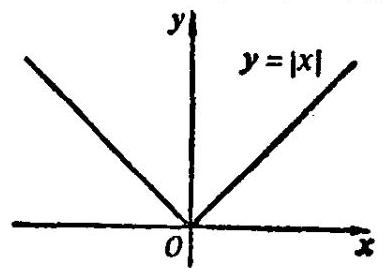
\includegraphics[max width=0.4\textwidth]{images/01912c18-5c3f-733d-b775-749ba9897a9d_69_933568.jpg}
\end{center}

图 2-3

*下面我们根据导数的定义证明 \(y = \left| x\right|\) 在 \(x = 0\) 处不可导. 并从而导出左、右导数的概念.

\(\because {\Delta y} = \left| {0 + {\Delta x}}\right| - \left| 0\right| = \left| {\Delta x}\right| = \left\{ \begin{array}{r} {\Delta x},\text{ 当 }{\Delta x} > 0, \\ - {\Delta x},\text{ 当 }{\Delta x} < 0, \end{array}\right.\)

\[
\therefore \mathop{\lim }\limits_{{{\Delta x} \rightarrow 0 + }}\frac{\Delta y}{\Delta x} = \mathop{\lim }\limits_{{{\Delta x} \rightarrow 0 + }}\frac{\Delta x}{\Delta x} = 1\text{,}
\]

\[
\mathop{\lim }\limits_{{{\Delta x} \rightarrow 0 - }}\frac{\Delta y}{\Delta x} = \mathop{\lim }\limits_{{{\Delta x} \rightarrow 0 - }}\frac{-{\Delta x}}{\Delta x} = - 1.
\]

也就是说,当 \({\Delta x} \rightarrow 0\) 时, \(\frac{\Delta y}{\Delta x}\) 的左、右极限不相等,所以 \(\frac{\Delta y}{\Delta x}\) 当 \({\Delta x} \rightarrow 0\) 时极限 不存在. 因此,函数 \(y = \left| x\right|\) 在点 \(x = 0\) 处不可导.

一般地,设已知函数 \(y = f\left( x\right) ,{\Delta y} = f\left( {{x}_{0} + {\Delta x}}\right) - f\left( {x}_{0}\right)\) ,如果 \(\frac{\Delta y}{\Delta x}\) 的左极限存在,就把左极限 \(\mathop{\lim }\limits_{{{\Delta x} \rightarrow 0}}\frac{\Delta y}{\Delta x}\) 叫做 \(f\left( x\right)\) 在点 \({x}_{0}\) 处的左导数; 如果 \(\frac{\Delta y}{\Delta x}\) 的右极限存在,就把右极限 \(\mathop{\lim }\limits_{{{\Delta x} \rightarrow 0 + }}\frac{\Delta y}{\Delta x}\) 叫做 \(f\left( x\right)\) 在点 \({x}_{0}\) 处的右导数.

根据左、右极限存在且相等是极限存在的充要条件, 可得左、右导数存在且相等是导数存在的充要条件.

如果函数 \(y = f\left( x\right)\) 在开区间 \(\left( {a,b}\right)\) 内可导,在左端点 \(x =\) \(a\) 处存在右导数,在右端点 \(x = b\) 处存在左导数,我们就说函数 \(f\left( x\right)\) 在闭区间 \(\left\lbrack {a,b}\right\rbrack\) 上可导.

\begin{problemset}[练习]

\item 先从函数的图象观察,然后根据定义判断函数 \(y = \sqrt[3]{{x}^{2}}\) 在点 \(x = 0\) 处是否连续,在点 \(x = 0\) 处是否可导.

\end{problemset}

\begin{problemset}[习 题 四]

\item 已知作直线运动的某一物体的运动方程为 \(s = \frac{5}{2}{t}^{2}\) (米), 当 \(t = 2\) 秒, \({\Delta t}\) 分别为 0.1 秒、 0.01 秒、 0.001 秒、 0.0001 秒、0.00001 秒时,求从 \({t}_{0}\) 到 \({t}_{0} + {\Delta t}\) 这段时间内的平均速度及 \(t = 2\) 秒时的瞬时速度.

\item 已知质点按规律 \(s = 2{t}^{2} + {4t}\) (米) 作直线运动,求:

(1)质点在运动开始后前 3 秒内的平均速度;

(2)质点在 2 秒到 3 秒内的平均速度;

(3)质点在 3 秒时的瞬时速度。

\item 求下列函数在指定点处的导数:

(1) \(y = {\left( x - 2\right) }^{2}\) ,点 \(x = 2\) ; (2) \(y = \frac{1}{x - 1}\) ,点 \(x = 0\) .

\item 说明函数 \(y = f\left( x\right)\) 在点 \({x}_{0}\) 处的导数也可定义为

\[
{f}^{\prime }\left( {x}_{0}\right) = \mathop{\lim }\limits_{{x \rightarrow {x}_{0}}}\frac{f\left( x\right) - f\left( {x}_{0}\right) }{x - {x}_{0}}.
\]

\item 求下列函数的导数:

(1) \(y = {ax} + b\) ; (2) \(y = \frac{1}{x}\)

(3) \(y = \frac{1}{{x}^{2}}\) (4) \(y = \frac{1}{\sqrt{x}}\) .

\item 已知 \(f\left( x\right) = \frac{1}{1 - x}\) ,求 \({f}^{\prime }\left( x\right) ,{f}^{\prime }\left( 0\right) ,{f}^{\prime }\left( 2\right)\) .

\item 已知 \(y = \sqrt{{a}^{2} - {x}^{2}}\) ,求证 \({y}^{\prime } = - \frac{x}{\sqrt{{a}^{2} - {x}^{2}}}\) .

\item 设质点 \(M\) 沿 \(x\) 轴作变速直线运动,在时刻 \(t\) (秒),质点 \(M\)

所在位置为 \(x = {t}^{2} - {5t} + 6\) (米). 求从 1 秒到 3 秒 这段时间内质点 \(M\) 的平均速度. 质点 \(M\) 在什么时刻的速度等于这段时间内的平均速度?

\item 求曲线 \(y = {2x} - {x}^{3}\) 在点 \(\left( {-1, - 1}\right)\) 处的切线的倾斜角.

\item 求抛物线 \(y = \frac{1}{4}{x}^{2}\) 在点 \(\left( {-2,1}\right)\) 及点 \(\left( {2,1}\right)\) 处的切线方程和法线方程。

\item 从时刻 \(t = 0\) 开始的 \(t\) 秒内,通过某导体的电量 (单位: 库仑)可由公式 \(q = 2{t}^{2} + {3t}\) 表示. 求第 5 秒时的电流强度及第 7 秒时的电流强度(即通过的电量 \(q\) 对时间 \(t\) 的导数 \({q}_{t}^{\prime }\) ),什么时刻电流强度达到 43 安培 (即库仑/秒).

\end{problemset}

\section*{求 导 方 法}

\section{几种常见函数的导数}

为了能够较快地求出某个函数的导数, 在下几节中我们将研究求导数的一般运算法则以及基本初等函数的导数公式. 这一节, 我们根据导数的定义先来证明几个常见函数的导数公式.

1. 设 \(y = C\) ( \(C\) 为常数),则 \({y}^{\prime } = 0\) .

证明:

\[
y = f\left( x\right) = C,
\]

\[
{\Delta y} = f\left( {x + {\Delta x}}\right) - f\left( x\right)
\]

\[
= C - C = 0,
\]

\[
\frac{\Delta y}{\Delta x} = 0
\]

\(\therefore \;{f}^{\prime }\left( x\right) = {C}^{\prime } = \mathop{\lim }\limits_{{{\Delta x} \rightarrow 0}}\frac{\Delta y}{\Delta x} = 0\) .

2. \({\left( {x}^{n}\right) }^{\prime } = n{x}^{n - 1}\) ( \(n\) 为正整数)

证明: \(y = f\left( x\right) = {x}^{n}\) ,

\[
{\Delta y} = f\left( {x + {\Delta x}}\right) - f\left( x\right)
\]

\[
= {\left( x + \Delta x\right) }^{n} - {x}^{n}
\]

\[
= \left\lbrack {{x}^{n} + {C}_{n}^{1}{x}^{n - 1}{\Delta x} + {C}_{n}^{2}{x}^{n - 2}{\left( \Delta x\right) }^{2}}\right.
\]

\[
\left. {+\cdots + {C}_{n}^{n}{\left( \Delta x\right) }^{n}}\right\rbrack - {x}^{n}
\]

\[
= {C}_{n}^{1}{x}^{n - 1}{\Delta x} + {C}_{n}^{2}{x}^{n - 2}{\left( \Delta x\right) }^{2} + \cdots + {C}_{n}^{n}{\left( \Delta x\right) }^{n},
\]

\[
\frac{\Delta y}{\Delta x} = {C}_{n}^{1}{x}^{n - 1} + {C}_{n}^{2}{x}^{n - 2}{\Delta x} + \cdots + {C}_{n}^{n}{\left( \Delta x\right) }^{n - 1},
\]

\[
\therefore \;{y}^{\prime } = {\left( {x}^{n}\right) }^{\prime } = \mathop{\lim }\limits_{{{\Delta x} \rightarrow 0}}\frac{\Delta y}{\Delta x}
\]

\[
= \mathop{\lim }\limits_{{{\Delta x} \rightarrow 0}}\left\lbrack {{C}_{n}^{1}{x}^{n - 1} + {C}_{n}^{2}{x}^{n - 2}{\Delta x} + \cdots + {C}_{n}^{n}{\left( \Delta x\right) }^{n - 1}}\right\rbrack
\]

\[
= n{x}^{n - 1}\text{. }
\]

例如,

\[
{\left( {x}^{3}\right) }^{\prime } = 3{x}^{2},\;{\left( {x}^{7}\right) }^{\prime } = 7{x}^{6},\;{\left( x\right) }^{\prime } = 1{x}^{0} = 1.
\]

3. \({\left( \sin x\right) }^{\prime } = \cos x\)

证明: \(y = \sin x\) ,

\[
{\Delta y} = \sin \left( {x + {\Delta x}}\right) - \sin x = 2\cos \left( {x + \frac{\Delta x}{2}}\right) \sin \frac{\Delta x}{2},
\]

\[
\frac{\Delta y}{\Delta x} = \cos \left( {x + \frac{\Delta x}{2}}\right) \frac{\sin \frac{\Delta x}{2}}{\frac{\Delta x}{2}}
\]

\(\because \;\mathop{\lim }\limits_{{{\Delta x} \rightarrow 0}}\frac{\sin \frac{\Delta x}{2}}{\frac{\Delta x}{2}} = 1\)

\(\therefore \;{y}^{\prime } = {\left( \sin x\right) }^{\prime } = \mathop{\lim }\limits_{{{\Delta x} \rightarrow 0}}\frac{\Delta y}{\Delta x}\)

\[
= \mathop{\lim }\limits_{{{\Delta x} \rightarrow 0}}\cos \left( {x + \frac{\Delta x}{2}}\right) \cdot \mathop{\lim }\limits_{{{\Delta x} \rightarrow 0}}\frac{\sin \frac{\Delta x}{2}}{\frac{\Delta x}{2}} = \cos x.
\]

4. \({\left( \cos x\right) }^{\prime } = - \sin x\)

请同学自己证明.

\begin{problemset}[练习]

\item (口答) 求下列函数的导数:

(1) \(y = {x}^{5}\) ; (2) \(y = {x}^{6}\) ;

(3) \(x = \sin t\) ; (4) \(u = \cos \varphi\) .

\end{problemset}

\section{函数的和、差、积、商的导数}

相应于函数极限的四则运算法则, 我们根据导数的定义来导出求导数的四则运算法则, 以简化求导数的计算. 在下面的公式中, \(u\) 及 \(v\) 都是 \(x\) 的函数,而且都是可导的.

\section*{1. 和(或差)的导数}

法则 1 两个函数的和 (或差) 的导数, 等于这两个函数的导数的和(或差). 即

\[
{\left( \mathbf{u} \pm \mathbf{v}\right) }^{\prime } = {\mathbf{u}}^{\prime } \pm \mathbf{v}.
\]

证明: \(y = f\left( x\right) = u\left( x\right) \pm v\left( x\right)\) ,

\[
{\Delta y} = \left\lbrack {u\left( {x + {\Delta x}}\right) \pm v\left( {x + {\Delta x}}\right) }\right\rbrack - \left\lbrack {u\left( x\right) \pm v\left( x\right) }\right\rbrack
\]

\[
= \left\lbrack {u\left( {x + {\Delta x}}\right) - u\left( x\right) }\right\rbrack \pm \left\lbrack {v\left( {x + {\Delta x}}\right) - v\left( x\right) }\right\rbrack
\]

\[
= {\Delta u} \pm {\Delta v}
\]

\[
\frac{\Delta y}{\Delta x} = \frac{\Delta u}{\Delta x} \pm \frac{\Delta v}{\Delta x}
\]

\[
\mathop{\lim }\limits_{{{\Delta x} \rightarrow 0}}\frac{\Delta y}{\Delta x} = \mathop{\lim }\limits_{{{\Delta x} \rightarrow 0}}\left( {\frac{\Delta u}{\Delta x} \pm \frac{\Delta v}{\Delta x}}\right) = \mathop{\lim }\limits_{{{\Delta x} \rightarrow 0}}\frac{\Delta u}{\Delta x} \pm \mathop{\lim }\limits_{{{\Delta x} \rightarrow 0}}\frac{\Delta v}{\Delta x}
\]

即

\[
{y}^{\prime } = {\left( u \pm v\right) }^{\prime } = {u}^{\prime } \pm {v}^{\prime }.
\]

这个法则可以推广到任意有限个函数, 即

\[
{\left( {u}_{1} \pm {u}_{2} \pm \cdots \pm {u}_{n}\right) }^{\prime } = {u}_{1}^{\prime } \pm {u}_{2}^{\prime } \pm \cdots \pm {u}_{n}^{\prime }.
\]

例 1 求 \(y = {x}^{3} + \sin x\) 的导数.

解: \({y}^{\prime } = {\left( {x}^{3}\right) }^{\prime } + {\left( \sin x\right) }^{\prime } = 3{x}^{2} + \cos x\) .

例 2 求 \(y = {x}^{4} - {x}^{2} - x + 3\) 的导数.

解: \({y}^{\prime } = 4{x}^{3} - {2x} - 1\) .

\section*{2. 积的导数}

法则 2 两个函数的积的导数, 等于第一个函数的导数乘以第二个函数, 加上第一个函数乘以第二个函数的导数. 即

\[
{\left( uv\right) }^{\prime } = {u}^{\prime }v + u{v}^{\prime }
\]

证明: \(y = f\left( x\right) = u\left( x\right) v\left( x\right)\) ,

\[
{\Delta y} = u\left( {x + {\Delta x}}\right) v\left( {x + {\Delta x}}\right) - u\left( x\right) v\left( x\right)
\]

\[
= u\left( {x + {\Delta x}}\right) v\left( {x + {\Delta x}}\right) - u\left( x\right) v\left( {x + {\Delta x}}\right)
\]

\[
+ u\left( x\right) v\left( {x + {\Delta x}}\right) - u\left( x\right) v\left( x\right)
\]

\[
\frac{\Delta y}{\Delta x} = \frac{u\left( {x + {\Delta x}}\right) - u\left( x\right) }{\Delta x}v\left( {x + {\Delta x}}\right) + u\left( x\right) \frac{v\left( {x + {\Delta x}}\right) - v\left( x\right) }{\Delta x}.
\]

因为 \(v\left( x\right)\) 在点 \(x\) 处可导,所以它在点 \(x\) 处连续,于是当 \({\Delta x} \rightarrow 0\) 时, \(v\left( {x + {\Delta x}}\right) \rightarrow v\left( x\right)\) . 从而

\[
\mathop{\lim }\limits_{{{\Delta x} \rightarrow 0}}\frac{\Delta y}{\Delta x} = \mathop{\lim }\limits_{{{\Delta x} \rightarrow 0}}\frac{u\left( {x + {\Delta x}}\right) - u\left( x\right) }{\Delta x}v\left( {x + {\Delta x}}\right)
\]

\[
+ u\left( x\right) \mathop{\lim }\limits_{{{\Delta x} \rightarrow 0}}\frac{v\left( {x + {\Delta x}}\right) - v\left( x\right) }{\Delta x}
\]

\[
= {u}^{\prime }v + u{v}^{\prime }
\]

即

\[
{y}^{\prime } = {\left( uv\right) }^{\prime } = {u}^{\prime }v + u{v}^{\prime }.
\]

从法则 2 立即可以得出

\[
{\left( Cu\right) }^{\prime } = {C}^{\prime }u + C{u}^{\prime } = 0 + C{u}^{\prime } = C{u}^{\prime },
\]

也就是, 常数与函数的积的导数, 等于常数乘以函数的导数.

即

\[
{\left( Cu\right) }^{\prime } = C{u}^{\prime }\text{. }
\]

例 3 求 \(y = 2{x}^{3} - 3{x}^{2} + {5x} - 4\) 的导数.

解: \({y}^{\prime } = 6{x}^{2} - {6x} + 5\) .

例 4 求 \(y = \left( {2{x}^{2} + 3}\right) \left( {{3x} - 2}\right)\) 的导数.

解: \({y}^{\prime } = {\left( 2{x}^{2} + 3\right) }^{\prime }\left( {{3x} - 2}\right) + \left( {2{x}^{2} + 3}\right) {\left( 3x - 2\right) }^{\prime }\)

\[
= {4x} \cdot \left( {{3x} - 2}\right) + \left( {2{x}^{2} + 3}\right) \cdot 3 = {18}{x}^{2} - {8x} + 9\text{.}
\]

\section*{3. 商的导数}

法则 3 两个函数的商的导数, 等于分子的导数 与分母的积, 减去分母的导数与分子的积, 再除以分母的平方. 即

\[
{\left( \frac{u}{v}\right) }^{\prime } = \frac{{u}^{\prime }v - u{v}^{\prime }}{{v}^{2}}\;\left( {v \neq 0}\right) .
\]

证明: \(y = f\left( x\right) = \frac{u\left( x\right) }{v\left( x\right) }\) ,

\[
{\Delta y} = \frac{u\left( {x + {\Delta x}}\right) }{v\left( {x + {\Delta x}}\right) } - \frac{u\left( x\right) }{v\left( x\right) }
\]

\[
= \frac{u\left( {x + {\Delta x}}\right) v\left( x\right) - u\left( x\right) v\left( {x + {\Delta x}}\right) }{v\left( {x + {\Delta x}}\right) v\left( x\right) }
\]

\[
= \frac{\left\lbrack {u\left( {x + {\Delta x}}\right) v\left( x\right) - u\left( x\right) v\left( x\right) }\right\rbrack - \left\lbrack {u\left( x\right) v\left( {x + {\Delta x}}\right) - u\left( x\right) v\left( x\right) }\right\rbrack }{v\left( {x + {\Delta x}}\right) v\left( x\right) }
\]

\[
= \frac{\left\lbrack {u\left( {x + {\Delta x}}\right) - u\left( x\right) }\right\rbrack v\left( x\right) - u\left( x\right) \left\lbrack {v\left( {x + {\Delta x}}\right) - v\left( x\right) }\right\rbrack }{v\left( {x + {\Delta x}}\right) v\left( x\right) }.
\]

\[
\frac{\Delta y}{\Delta x} = \frac{\frac{u\left( {x + {\Delta x}}\right) - u\left( x\right) }{\Delta x}v\left( x\right) - u\left( x\right) \frac{v\left( {x + {\Delta x}}\right) - v\left( x\right) }{\Delta x}}{v\left( {x + {\Delta x}}\right) v\left( x\right) }.
\]

因为 \(v\left( x\right)\) 在点 \(x\) 处可导,所以它在点 \(x\) 处连续,于是当 \({\Delta x} \rightarrow 0\) 时, \(v\left( {x + {\Delta x}}\right) \rightarrow v\left( x\right)\) . 从而

\[
\mathop{\lim }\limits_{{{\Delta x} \rightarrow 0}}\frac{\Delta y}{\Delta x} = \frac{{u}^{\prime }\left( x\right) v\left( x\right) - u\left( x\right) {v}^{\prime }\left( x\right) }{{\left\lbrack v\left( x\right) \right\rbrack }^{2}},
\]

即

\[
{y}^{\prime } = {\left( \frac{u}{v}\right) }^{\prime } = \frac{{u}^{\prime }v - u{v}^{\prime }}{{v}^{2}}.
\]

例 5 求 \(y = \frac{{x}^{2}}{\sin x}\) 的导数.

解: \({y}^{\prime } = \frac{{\left( {x}^{2}\right) }^{\prime } \cdot \sin x - {x}^{2} \cdot {\left( \sin x\right) }^{\prime }}{{\sin }^{2}x} = \frac{{2x}\sin x - {x}^{2}\cos x}{{\sin }^{2}x}\) .

例 6 求 \(y = \frac{x + 3}{{x}^{2} + 3}\) 在点 \(x = 3\) 处的导数.

解: \({y}^{\prime } = \frac{1 \cdot \left( {{x}^{2} + 3}\right) - \left( {x + 3}\right) \cdot {2x}}{{\left( {x}^{2} + 3\right) }^{2}} = \frac{-{x}^{2} - {6x} + 3}{{\left( {x}^{2} + 3\right) }^{2}}\) ,

\[
\therefore {\left. {y}^{\prime }\right| }_{x = 3} = \frac{-9 - {18} + 3}{{\left( 9 + 3\right) }^{2}} = \frac{-{24}}{144} = - \frac{1}{6}\text{.}
\]

例 7 求证当 \(n\) 是负整数时,公式

\[
{\left( {x}^{n}\right) }^{\prime } = n{x}^{n - 1}
\]

仍然成立.

证明: 设 \(n = - m\) ,则 \(m\) 为正整数.

\[
\therefore \;{\left( {x}^{n}\right) }^{\prime } = {\left( {x}^{-m}\right) }^{\prime } = {\left( \frac{1}{{x}^{m}}\right) }^{\prime }
\]

\[
= \frac{0 \cdot {x}^{m} - m{x}^{m - 1}}{{x}^{2m}}
\]

\[
= - m{x}^{-m - 1} = n{x}^{n - 1}.
\]

例 8 求 \(y = 2{x}^{2} - {3x} + 4 - \frac{3}{x} + \frac{2}{{x}^{2}}\) 的导数.

解: \(y = 2{x}^{2} - {3x} + 4 - 3{x}^{-1} + 2{x}^{-2}\) ,

\[
\therefore \;{y}^{\prime } = {4x} - 3 + 3{x}^{-2} - 4{x}^{-3}
\]

\[
= {4x} - 3 + \frac{3}{{x}^{2}} - \frac{4}{{x}^{3}}
\]

\begin{problemset}[练习]

\item 求下列函数的导数:

(1) \(y = 3{x}^{4} - {23}{x}^{3} + {40x} - {10}\) ; \(\;\left( 2\right) y = a{x}^{3} - {bx} + c\) ;

(3) \(y = \sin x - x + 1\) ; (4) \(y = {x}^{2} + 2\cos x\) .

\item 填空:

(1) \({\left\lbrack \left( 3{x}^{2} + 1\right) \left( 4{x}^{2} - 3\right) \right\rbrack }^{\prime }\)

\(= \left( \;\right) \left( {4{x}^{2} - 3}\right) + \left( {3{x}^{2} + 1}\right) \left( \;\right)\) ;

(2) \({\left( {x}^{3}\sin x\right) }^{\prime } = \left( \;\right) {x}^{2}\sin x + {x}^{3}\left( \;\right)\) .

\item 求下列函数的导数:

(1) \(y = \left( {3{x}^{2} + 1}\right) \left( {2 - x}\right)\) ; (2) \(y = \left( {1 - 2{x}^{3}}\right) \left( {x - 3{x}^{2}}\right)\) ;

(3) \(y = \left( {1 + {x}^{2}}\right) \cos x\) ; (4) \(y = \left( {1 + \sin x}\right) \left( {1 - {2x}}\right)\) .

\item 填空:

(1) \({\left( \frac{x}{{x}^{2} + 1}\right) }^{\prime } = \frac{\left( \;\right) \left( {{x}^{2} + 1}\right) - x\left( \;\right) }{{\left( {x}^{2} + 1\right) }^{2}}\)

(2) \({\left( \frac{1 - {x}^{2}}{\sin x}\right) }^{\prime } = \frac{\left( \;\right) \sin x - \left( {1 - {x}^{2}}\right) \left( \;\right) }{{\sin }^{2}x}\) .

\item 求下列函数的导数:

(1) \(y = \frac{a - x}{a + x}\) (2) \(y = \frac{1 + x}{3 - {x}^{2}}\)

(3) \(y = \frac{\cos x}{1 - {x}^{2}}\) (4) \(y = \frac{1}{1 + \sin x}\) ;

(5) \(y = 1 + \frac{2}{x} + \frac{3}{{x}^{2}} - \frac{4}{{x}^{3}}\) (6) \(y = \frac{-3{x}^{4} + 3{x}^{2} - 5}{{x}^{3}}\) .

\item 下列做法是否正确? 如果不正确, 加以改正:

(1) \({\left\lbrack \left( 3 + {x}^{2}\right) \left( 2 - {x}^{3}\right) \right\rbrack }^{\prime } = {2x}\left( {2 - {x}^{3}}\right) + 3{x}^{2}\left( {3 + {x}^{2}}\right)\) ;

(2) \({\left( \frac{1 + \cos x}{{x}^{2}}\right) }^{\prime } = \frac{{2x}\left( {1 + \cos x}\right) + {x}^{2}\sin x}{{x}^{2}}\) .

\end{problemset}

\section{复合函数的导数}

我们先看一个例子. 设已知

\[
y = {\left( 3x - 2\right) }^{2},
\]

那么,

\[
{y}^{\prime } = {\left\lbrack {\left( 3x - 2\right) }^{2}\right\rbrack }^{\prime } = {\left( 9{x}^{2} - {12}x + 4\right) }^{\prime } = {18x} - {12}.
\]

函数 \(y = {\left( 3x - 2\right) }^{2}\) 又可以看成由

\[
y = {u}^{2},u = {3x} - 2
\]

复合而成的. 由于

\[
{y}_{u}^{\prime } = {2u},\;{u}_{x}^{\prime } = 3,
\]

因而

\[
{y}_{u}^{\prime } \cdot {u}_{x}^{\prime } = {2u} \cdot 3 = 2\left( {{3x} - 2}\right) \cdot 3 = {18x} - {12}.
\]

于是在本例中, 我们有等式

\[
{y}_{x}^{\prime } = {y}_{u}^{\prime } \cdot {u}_{x}^{\prime }
\]

一般地,设函数 \(u = \varphi \left( x\right)\) 在点 \(x\) 处有导数 \({u}_{x}^{\prime } = {\varphi }^{\prime }\left( x\right)\) , 函数 \(y = f\left( u\right)\) 在点 \(x\) 的对应点 \(u\) 处有导数 \({y}_{u}^{\prime } = {f}^{\prime }\left( u\right)\) ,则复合函数 \(y = f\left\lbrack {\varphi \left( x\right) }\right\rbrack\) 在点 \(x\) 处也有导数,且

\[
{y}_{x}^{\prime } = {y}_{u}^{\prime } \cdot {u}_{x}^{\prime }
\]

或写作

\[
{f}_{x}^{\prime }\left\lbrack {\varphi \left( x\right) }\right\rbrack = {f}^{\prime }\left( u\right) {\varphi }^{\prime }\left( x\right) .
\]

证明: 设 \(x\) 有一改变量 \({\Delta x}\) ,则对应的 \(u\text{、}y\) 分别有改变量 \({\Delta u}\text{、}{\Delta y}\) . 因为 \(u = \varphi \left( x\right)\) 在点 \(x\) 处可导,所以 \(u = \varphi \left( x\right)\) 在点 \(x\) 处连续. 因此当 \({\Delta x} \rightarrow 0\) 时, \({\Delta u} \rightarrow 0\) . 设 \({\Delta u} \neq 0\mathbf{0}\) ,由

\[
\frac{\Delta y}{\Delta x} = \frac{\Delta y}{\Delta u} \cdot \frac{\Delta u}{\Delta x}
\]

且

\[
\mathop{\lim }\limits_{{{\Delta x} \rightarrow 0}}\frac{\Delta y}{\Delta u} = \mathop{\lim }\limits_{{{\Delta u} \rightarrow 0}}\frac{\Delta y}{\Delta u}
\]

得

\[
\mathop{\lim }\limits_{{{\Delta x} \rightarrow 0}}\frac{\Delta y}{\Delta x} = \mathop{\lim }\limits_{{{\Delta x} \rightarrow 0}}\frac{\Delta y}{\Delta u} \cdot \mathop{\lim }\limits_{{{\Delta x} \rightarrow 0}}\frac{\Delta u}{\Delta x}
\]

3 \({\Delta u} = 0\) 时公式也成立,证明从略.

\[
= \mathop{\lim }\limits_{{{\Delta u} \rightarrow 0}}\frac{\Delta y}{\Delta u} \cdot \mathop{\lim }\limits_{{{\Delta x} \rightarrow 0}}\frac{\Delta u}{\Delta x}
\]

即

\[
{y}_{x}^{\prime } = {y}_{u}^{\prime } \cdot {u}_{x}^{\prime }
\]

这就是复合函数的求导法则, 即: 复合函数对自变量的导数, 等于已知函数对中间变量的导数, 乘以中间变量对自变量的导数.

这个法则可以推广到两个以上的中间变量. 例如, 如果

\[
y = y\left( u\right) ,u = u\left( v\right) ,v = v\left( x\right) ,
\]

那么有

\[
{y}_{x}^{\prime } = {y}_{u}^{\prime } \cdot {u}_{v}^{\prime } \cdot {v}_{x}^{\prime }
\]

例 1 求 \(y = {\left( 2x + 1\right) }^{5}\) 的导数.

解: 设 \(y = {u}^{5},u = {2x} + 1\) .

根据复合函数求导法则, 有

\[
{y}_{x}^{\prime } = {y}_{u}^{\prime } \cdot {u}_{x}^{\prime } = {\left( {u}^{5}\right) }_{u}^{\prime } \cdot {\left( 2x + 1\right) }_{x}^{\prime }
\]

\[
= 5{u}^{4} \cdot 2 = 5{\left( 2x + 1\right) }^{4} \cdot 2
\]

\[
= {10}{\left( 2x + 1\right) }^{4}\text{.}
\]

注意: 在利用复合函数的求导法则求导数后, 要把中间变量换成自变量的函数.

例 2 求 \(y = \frac{1}{{\left( 1 - 3x\right) }^{4}}\) 的导数.

解: \(y = \frac{1}{{\left( 1 - 3x\right) }^{4}} = {\left( 1 - 3x\right) }^{-4}\) .

设 \(y = {u}^{-4},u = \left( {1 - {3x}}\right)\) ,则

\[
{y}_{x}^{\prime } = {y}_{u}^{\prime } \cdot {u}_{x}^{\prime }
\]

\[
= {\left( {u}^{-4}\right) }_{u}^{\prime } \cdot {\left( 1 - 3x\right) }_{x}^{\prime }
\]

\[
= - 4{u}^{-5} \cdot \left( {-3}\right)
\]

\[
= {12}{u}^{-5}
\]

\[
= {12}{\left( 1 - 3x\right) }^{-5}
\]

\[
= \frac{12}{{\left( 1 - 3x\right) }^{5}}
\]

例 3 求 \(y = {\sin }^{2}\left( {{2x} + \frac{\pi }{3}}\right)\) 的导数.

解: 设 \(y = {u}^{2},u = \sin v,v = {2x} + \frac{\pi }{3}\) ,

\[
{y}_{x}^{\prime } = {y}_{u}^{\prime } \cdot {u}_{v}^{\prime } \cdot {v}_{x}^{\prime }
\]

\[
= {\left( {u}^{2}\right) }_{u}^{\prime } \cdot {\left( \sin v\right) }_{v}^{\prime } \cdot {\left( 2x + \frac{\pi }{3}\right) }_{x}^{\prime }
\]

\[
= {2u} \cdot \cos v \cdot 2
\]

\[
= 2\sin \left( {{2x} + \frac{\pi }{3}}\right) \cdot \cos \left( {{2x} + \frac{\pi }{3}}\right) \cdot 2
\]

\[
= 2\sin \left( {{4x} + \frac{2\pi }{3}}\right) \text{.}
\]

求复合函数的导数, 关键在于分析清楚函数的复合关系, 适当选定中间变量, 明确每次是哪个变量对哪个变量求导数. 在熟练以后, 就不必再写出中间步骤. 如以上三例可分别直接写成

\[
{y}^{\prime } = {\left\lbrack {\left( 2x + 1\right) }^{5}\right\rbrack }^{\prime } = 5{\left( 2x + 1\right) }^{4} \cdot 2 = {10}{\left( 2x + 1\right) }^{4}.
\]

\[
{y}^{\prime } = {\left\lbrack {\left( 1 - 3x\right) }^{-4}\right\rbrack }^{\prime } = - 4{\left( 1 - 3x\right) }^{-5} \cdot \left( {-3}\right) = {12}{\left( 1 - 3x\right) }^{-5}.
\]

\[
{y}^{\prime } = {\left\lbrack {\sin }^{2}\left( 2x + \frac{\pi }{3}\right) \right\rbrack }^{\prime } = 2\sin \left( {{2x} + \frac{\pi }{3}}\right) \cdot \cos \left( {{2x} + \frac{\pi }{3}}\right) \cdot 2
\]

\[
= 2\sin \left( {{4x} + \frac{2\pi }{3}}\right)
\]

对经过多次复合及四则运算而成的复合函数, 也可利用复合函数的求导法则, 由外向里, 逐层求导.

例 4 求 \(y = {\left( at - b{\sin }^{2}\omega t\right) }^{3}\) 对 \(t\) 的导数.

解: \({y}^{\prime } = 3{\left( at - b{\sin }^{2}\omega t\right) }^{2} \cdot {\left( at - b{\sin }^{2}\omega t\right) }^{\prime }\)

\[
= 3{\left( at - b{\sin }^{2}\omega t\right) }^{2}\left\lbrack {a - {2b}\sin {\omega t} \cdot {\left( \sin \omega t\right) }^{\prime }}\right\rbrack
\]

\[
= 3{\left( at - b{\sin }^{2}\omega t\right) }^{2}\left\lbrack {a - {2b}\sin {\omega t} \cdot \cos {\omega t} \cdot {\left( \omega t\right) }^{\prime }}\right\rbrack
\]

\[
\sim 3{\left( at - b{\sin }^{2}\omega t\right) }^{2}\left( {a - {2b}\sin {\omega t} \cdot \cos {\omega t} \cdot \omega }\right)
\]

\[
= 3{\left( at - b{\sin }^{2}\omega t\right) }^{2}\left( {a - {b\omega }\sin {2\omega t}}\right) \text{.}
\]

熟练以后, 也可省去中间步骤, 直接写成

\[
{y}^{\prime } = 3{\left( at - b{\sin }^{2}\omega t\right) }^{2}\left( {a - {2b}\sin {\omega t} \cdot \cos {\omega t} \cdot \omega }\right)
\]

\[
= 3{\left( at - b{\sin }^{2}\omega t\right) }^{2}\left( {a - {b\omega }\sin {2\omega t}}\right) \text{.}
\]

在 2.12 节我们将要证明,公式 \({\left( {x}^{a}\right) }^{\prime } = \alpha {x}^{a - 1}\) 对一切实数 \(\alpha\) 都成立. 现在先运用这个公式和复合函数的求导法则来求一些无理函数的导数 (中间步骤省略不写).

例 5 求 \(y = \sqrt[3]{a{x}^{2} + {bx} + c}\) 的导数.

解: \(y = \sqrt[3]{a{x}^{2} + {bx} + c} = {\left( a{x}^{2} + bx + c\right) }^{\frac{1}{3}}\) ,

\[
\therefore \;{y}^{\prime } = \frac{1}{3}{\left( a{x}^{2} + bx + c\right) }^{-\frac{2}{3}} \cdot \left( {{2ax} + b}\right)
\]

\[
= \frac{{2ax} + b}{3\sqrt[3]{{\left( a{x}^{2} + bx + c\right) }^{2}}}.
\]

例 6 求 \(y = \left( {2{x}^{2} - 3}\right) \sqrt{1 + {x}^{2}}\) 的导数.

解: \(y = \left( {2{x}^{2} - 3}\right) \sqrt{1 + {x}^{2}} = \left( {2{x}^{2} - 3}\right) {\left( 1 + {x}^{2}\right) }^{\frac{1}{2}}\) ,

\[
\therefore \;{y}^{\prime } = {4x} \cdot {\left( 1 + {x}^{2}\right) }^{\frac{1}{2}} + \left( {2{x}^{2} - 3}\right) \cdot \frac{1}{2}{\left( 1 + {x}^{2}\right) }^{-\frac{1}{2}} \cdot {2x}
\]

\[
= {4x}\sqrt{1 + {x}^{2}} + \frac{x\left( {2{x}^{2} - 3}\right) }{\sqrt{1 + {x}^{2}}}
\]

\[
= \frac{{4x}\left( {1 + {x}^{2}}\right) + x\left( {2{x}^{2} - 3}\right) }{\sqrt{1 + {x}^{2}}}
\]

\[
= \frac{6{x}^{3} + x}{\sqrt{1 + {x}^{2}}}
\]

\begin{problemset}[练习]

\item 把下列函数看成由一些比较简单的函数复合而成的, 写出它们的复合过程:

(1) \(y = {\left( {x}^{2} - 1\right) }^{3}\) ; (2) \(y = \operatorname{tg}\left( {\frac{\pi }{4} - x}\right)\)

(3) \(y = {e}^{1 + {x}^{2}}\) (4) \(y = \sin \frac{1}{\sqrt{1 + {x}^{2}}}\) .

\item 按例 1 中的步骤, 对下列函数, 先设中间变量, 然后求导:

(1) \(y = {\left( 5x - 3\right) }^{4}\) ; (2) \(y = {\left( 2 - {x}^{2}\right) }^{3}\) ;

(3) \(y = \sin \left( {{3x} - \frac{\pi }{6}}\right)\) ; (4) \(y = \cos \left( {1 + {x}^{2}}\right)\) .

\item 填空:

(1) \({y}^{\prime } = {\left\lbrack {\left( 2{x}^{3} + x\right) }^{2}\right\rbrack }^{\prime } = 2\left( {2{x}^{3} + x}\right) \left( \;\right)\) ;

(2) \({y}^{\prime } = {\left\lbrack {\left( 1 + {x}^{2}\right) }^{2}\sin \left( ax + b\right) \right\rbrack }^{\prime }\)

\[
= 2\left( {1 + {x}^{2}}\right) \left( \;\right) \sin \left( {{ax} + b}\right)
\]

\[
+ {\left( 1 + {x}^{2}\right) }^{2}\cos \left( {{ax} + b}\right) \left( \;\right) \text{; }
\]

(3) \({y}^{\prime } = {\left\lbrack {\left( 1 + {\cos }^{2}x\right) }^{3}\right\rbrack }^{\prime } = 3{\left( 1 + {\cos }^{2}x\right) }^{2}\left( \;\right) \left( \;\right)\) ;

(4) \({y}^{\prime } = {\left\lbrack \frac{1}{{\left( 2 + 3x\right) }^{5}}\right\rbrack }^{\prime } = {\left\lbrack {\left( 2 + 3x\right) }^{-5}\right\rbrack }^{\prime }\)

\[
= \left( \;\right) {\left( 2 + 3x\right) }^{-6}\left( \;\right) \text{. }
\]

\item 求下列函数的导数:

(1) \(y = \sin {x}^{2} - \sin {3x}\) ; (2) \(y = \frac{{x}^{2}}{{\left( 2x + 1\right) }^{3}}\) ;

(3) \(y = {x}^{2}\sqrt{x} - \frac{1}{\sqrt{x}}\) (4) \(y = \sqrt{{x}^{2} - {a}^{2}}\) ;

(5) \(y = \frac{1}{\sqrt[3]{{x}^{2} - 1}}\) (6) \(y = \sqrt{{4x} + 3}\cos {2x}\) .
\end{problemset}

\begin{problemset}[习 题 五]

\item 求下列函数的导数:

(1) \(y = {x}^{2}\sin x + {x}^{3}\) ; (2) \(y = \frac{{a}^{2} - {x}^{2}}{{a}^{2} + {x}^{2}}\)

(3) \(y = \left( {2 + {3x}}\right) \left( {1 - x + {x}^{2}}\right)\) ; (4) \(y = \frac{\cos x}{1 - \sin x}\) ;

(5) \(y = {x}^{3}\left( {\sin x + \sin \frac{\pi }{4}}\right)\) ; (6) \(y = \frac{x - 1}{{x}^{2} - {3x} + 6}\) .

\item 已知 \(u,v,w\) 是 \(x\) 的可导函数,求证

\[
{\left( uvw\right) }^{\prime } = {u}^{\prime }{vw} + u{v}^{\prime }w + {uv}{w}^{\prime }.
\]

\item 求下列函数在指定点处的导数:

(1) \(y = x\sin x\) 在点 \(x = \frac{\pi }{4}\) 处;

(2) \(y = \frac{2 - 3{x}^{2}}{1 + {2x}}\) 在点 \(x = 1\) 处.

\item 求正弦函数 \(y = \sin x\) 在点 \(\left( {\frac{\pi }{6},\frac{1}{2}}\right)\) 处的切线方程和法线方程.

\item 已知曲线 \(y = {x}^{3} + {3x}\) ,求这条曲线平行于直线 \(y = {15x} + 2\) 的切线的方程.

\item 已知曲线 \(y = 2{x}^{3} + 3{x}^{2} - {12x} + 1\) ,求这条曲线的与 \(x\) 轴平行的切线的方程.

\item 已知曲线 \(y = {x}^{3} + {x}^{2} - 1\) ,在曲线上哪一点处作切线,它的倾斜角等于 \({45}^{ \circ }\) ? 求在这点处的切线和法线的方程.

\item 已知函数 \(f\left( x\right) = {x}^{2}\left( {x - 1}\right)\) 当 \(x = {x}_{0}\) 时有 \({f}^{\prime }\left( {x}_{0}\right) = f\left( {x}_{0}\right)\) , 求 \({x}_{0}\) 的值.

\item 已知两个作直线运动的物体的运动方程 \({s}_{1}\left( t\right) = \frac{1}{3}{t}^{3}\) 及 \({s}_{2}\left( t\right) = {20t} - 4{t}^{2}\;\left( {t \geq 0}\right)\) ,在什么时刻它们运动的速度相等?

\item 在直线轨道上运行的一列火车, 从刹车到停车这段时间内,测得刹车后 \(t\) 秒内列车前进的距离 \(s = {27t} - {0.45}{t}^{2}\) (单位是米). 这列车在刹车后几秒钟才停车? 刹车后又运行了多少米?

\item 求下列函数的导数:

(1) \(y = {x}^{2}\sqrt{x} - 3\sqrt{x} + \frac{1}{x\sqrt{x}}\) ;

(2) \(y = \frac{3{x}^{3} - {x}^{2} + {5x} - 2}{\sqrt[3]{x}}\) .

\item 把下列函数看成由一些比较简单的函数复合而成的, 写出它们的复合过程:

(1) \(y = \frac{1}{\sqrt[5]{1 + {3x}}}\) (2) \(y = \arcsin \frac{1 - x}{1 + x}\)

(3) \({}^{1}y = \lg \sin \sqrt{x}\) ; (4) \(y = \sqrt{3 + \cos {2x}}\) .

\item 对下列函数, 先设中间变量, 然后求导:

(1) \(y = {\left( ax + b\right) }^{n}\) ; (2) \(y = \sqrt{2 - {x}^{2}}\) ;

(3) \(y = {\sin }^{3}\left( {{4x} + 3}\right)\) .

\item 求下列函数的导数:

(1) \(y = {\left( 2x - 1\right) }^{2}{\left( 2 - 3x\right) }^{3}\) ; (2) \(y = \frac{1}{{\left( a + b{x}^{2}\right) }^{3}}\) ;

(3) \(y = \frac{x}{\sqrt{1 + x}}\) (4) \(y = 2{\sin }^{2}\frac{x}{2} - \sqrt{x}\) ;

(5) \(y = \sqrt[3]{1 + {x}^{2}}\sin {5x}\) ; (6) \(y = {\left( \frac{x}{1 + x}\right) }^{5}\) ;

(7) \(y = \frac{x}{2}\sqrt{{a}^{2} - {x}^{2}}\) ; (8) \(y = \frac{x}{\sqrt{{x}^{2} - {a}^{2}}}\) .

\item 求下列曲线在指定点 \(M\) 处的切线和法线的方程:

(1) \(y = \frac{3}{5}\sqrt{{25} - {x}^{2}}\) ,点 \(M\left( {4,\frac{9}{5}}\right)\) ;

(2) \(y = {x}^{2} - 4\sqrt{x}\) ,点 \(M\left( {1, - 3}\right)\) .

\item 把 \(y = \frac{u}{v}\) (其中 \(u,v\) 都是 \(x\) 的函数, \(v \neq 0\) ) 改写成 \(y =\) \(u{v}^{-1}\) ,利用积的求导法则和复合函数的求导法则,导出商的求导法则 \({\left( \frac{u}{v}\right) }^{\prime } = \frac{{u}^{\prime }v - u{v}^{\prime }}{{v}^{2}}\) .

\end{problemset}

\section{三角函数的导数}

1. \({\left( \sin x\right) }^{\prime } = \cos x\)

这一公式根据定义已证明.

现在, 利用复合函数求导法则以及和、差、积、商的求导法则, 可以简便地推导出余弦函数、正切函数及余切函数的导数公式.

2. \({\left( \cos x\right) }^{\prime } = - \sin x\)

证明: \({\left( \cos x\right) }^{\prime } = {\left\lbrack \sin \left( \frac{\pi }{2} - x\right) \right\rbrack }^{\prime }\)

\[
= - \cos \left( {\frac{\pi }{2} - x}\right) = - \sin x\text{. }
\]

3. \({\left( \operatorname{tg}x\right) }^{\prime } = {\sec }^{2}x\)

证明: \({\left( \operatorname{tg}x\right) }^{\prime } = {\left( \frac{\sin x}{\cos x}\right) }^{\prime }\)

\[
= \frac{\cos x\cos x - \sin x\left( {-\sin x}\right) }{{\cos }^{2}x}
\]

\[
= \frac{1}{{\cos }^{2}x} = {\sec }^{2}x\text{. }
\]

4. \({\left( \operatorname{ctg}x\right) }^{\prime } = - {\csc }^{2}x\)

这个公式由同学自己证明.

例 1 求证:

\[
{\left( \sec x\right) }^{\prime } = \sec x\operatorname{tg}x
\]

\[
{\left( \csc x\right) }^{\prime } = - \csc x\operatorname{ctg}x\text{. }
\]

证明: \({\left( \sec x\right) }^{\prime } = {\left\lbrack {\left( \cos x\right) }^{-1}\right\rbrack }^{\prime }\)

\[
= - {\left( \cos x\right) }^{-2}\left( {-\sin x}\right)
\]

\[
= \frac{1}{\cos x} \cdot \frac{\sin x}{\cos x}
\]

\[
= \sec x\operatorname{tg}x
\]

\[
{\left( \csc x\right) }^{\prime } = {\left\lbrack {\left( \sin x\right) }^{-1}\right\rbrack }^{\prime }
\]

\[
= - {\left( \sin x\right) }^{-2} \cdot \cos x
\]

\[
= - \frac{1}{\sin x} \cdot \frac{\cos x}{\sin x}
\]

\[
= - \csc x\operatorname{ctg}x\text{.}
\]

例 2 求 \(y = \sin {nx}{\sin }^{n}x\) 的导数.

解: \({y}^{\prime } = n\cos {nx} \cdot \sin {}^{n}x + \sin {nx} \cdot n\sin {}^{n - 1}x\cos x\)

\[
= n{\sin }^{n - 1}x\left( {\cos {nx}\sin x + \sin {nx}\cos x}\right)
\]

\[
= n{\sin }^{n - 1}x\sin \left( {n + 1}\right) x\text{. }
\]

例 3 求 \(y = \sin \left( {x + \alpha }\right) \sin \left( {x - \alpha }\right)\) 的导数.

解: \(y = - \frac{1}{2}\left( {\cos {2x} - \cos {2\alpha }}\right)\) .

\[
{y}^{\prime } = - \frac{1}{2}\left( {-\sin {2x} \cdot 2}\right) = \sin {2x}.
\]

例 4 求 \(y = \operatorname{tg}\sqrt{1 - x}\) 的导数.

解: \({y}^{\prime } = {\sec }^{2}\sqrt{1 - x} \cdot {\left( \sqrt{1 - x}\right) }^{\prime }\)

\[
= {\sec }^{2}\sqrt{1 - x} \cdot \frac{-1}{2\sqrt{1 - x}}
\]

\[
= - \frac{{\sec }^{2}\sqrt{1 - x}}{2\sqrt{1 - x}}
\]

\begin{problemset}[练习]

\item 求下列函数的导数:

(1) \(f\left( \theta \right) = \frac{1 + \cos \theta }{1 - \cos \theta }\) (2) \(y = \cos {x}^{2} - \sin \sqrt{x}\) ;

(3) \(f\left( \theta \right) = \operatorname{tg}\theta - \theta\) ; (4) \(y = \operatorname{tg}\frac{x}{2} - \operatorname{ctg}\frac{x}{2}\) .

\end{problemset}

\section{反三角函数的导数}

反正弦函数与正弦函数互为反函数. 已知正弦函数的导数, 能否从而求出反正弦函数的导数呢?

下面, 我们先来研究互为反函数的两个函数的导数之间的关系.

\section*{1. 反函数的导数}

我们来看一个例子. 设

\[
y = {2x} - 3,
\]

则

\[
{y}_{x}^{\prime } = {\left( 2x - 3\right) }_{x}^{\prime } = 2.
\]

\(y = {2x} - 3\) 的反函数是 \(x = \frac{y + 3}{2}\) (这里 \(y\) 是自变量, \(x\) 是 \(y\) 的函数),

\[
{x}_{y}^{\prime } = {\left( \frac{y + 3}{2}\right) }_{y}^{\prime } = \frac{1}{2}
\]

因此, 在本例中我们有

\[
{y}_{x}^{\prime } = \frac{1}{{x}_{y}^{\prime }}.
\]

一般地,如果函数 \(y = f\left( x\right)\) 与 \(x = \varphi \left( y\right)\) 互为反函数,它们的导数是不是也有上述关系呢?

设已知函数 \(y = f\left( x\right)\) 是 \(x = \varphi \left( y\right)\) 的反函数, \(y = f\left( x\right)\) 在点 \(x\) 处连续, \(x = \varphi \left( y\right)\) 在对应点 \(y\) 处的导数不等于零. 给 \(x\) 以改变量 \({\Delta x}\) ,相应地 \(y = f\left( x\right)\) 就有改变量

\[
{\Delta y} = f\left( {x + {\Delta x}}\right) - f\left( x\right) .
\]

当 \({\Delta x} \neq 0\) 时,一定有 \({\Delta y} \neq 0\) ,否则不等的两个值 \(x\) 与 \(x + {\Delta x}\) 将对应同一函数值 \(y\) ,这和 “ \(y = f\left( x\right)\) 与 \(x = \varphi \left( y\right)\) 互为反函数” 矛盾. 因此

\[
\frac{\Delta y}{\Delta x} = \frac{1}{\frac{\Delta x}{\Delta y}}
\]

由于 \(y = f\left( x\right)\) 在点 \(x\) 处连续,即当 \({\Delta x} \rightarrow 0\) 时, \({\Delta y} \rightarrow 0\) ,又由于 \(x = \varphi \left( y\right)\) 在对应点 \(y\) 处有不等于零的导数,所以

\[
\mathop{\lim }\limits_{{{\Delta x} \rightarrow 0}}\frac{\Delta y}{\Delta x} = \mathop{\lim }\limits_{{{\Delta y} \rightarrow 0}}\frac{1}{\frac{\Delta x}{\Delta y}} = \frac{1}{\mathop{\lim }\limits_{{{\Delta y} \rightarrow 0}}\frac{\Delta x}{\Delta y}} = \frac{1}{{x}_{y}^{\prime }},
\]

即有

\[
{y}_{x}^{\prime } = \frac{1}{{x}_{y}^{\prime }}.
\]

于是, 我们得到反函数的求导法则如下:

已知函数 \(y = f\left( x\right)\) 是函数 \(x = \varphi \left( y\right)\) 的反函数, \(y = f\left( x\right)\) 在点 \(x\) 处连续, \(x = \varphi \left( y\right)\) 在对应点 \(y\) 处的导数不等于零,那么, \(y = f\left( x\right)\) 在点 \(x\) 处有导数,且

\[
{y}_{x}^{\prime } = \frac{1}{{x}_{y}^{\prime }}\text{.}
\]

或记作

\[
{f}^{\prime }\left( x\right) = \frac{1}{{\varphi }^{\prime }\left( y\right) }
\]

\section*{2. 反三角函数的导数}

根据反函数的求导法则, 我们可以得出反三角函数的导数公式如下:

(1) \({\left( \arcsin x\right) }^{\prime } = \frac{1}{\sqrt{1 - {x}^{2}}}\)

证明: 设 \(y = \arcsin x\left( {-1 \leq x \leq 1}\right)\) ,则

\[
x = \sin y\left( {-\frac{\pi }{2} \leq y \leq \frac{\pi }{2}}\right) .
\]

\(y = \arcsin x\) 在 \(\left( {-1 < x < 1}\right)\) 上连续,且当 \(- \frac{\pi }{2} < y < \frac{\pi }{2}\) 时, \({x}_{y}^{\prime } = \cos y > 0\) ,这时,由反函数的求导法则,有

\[
{y}_{x}^{\prime } = \frac{1}{{x}_{y}^{\prime }} = \frac{1}{{\left( \sin y\right) }^{\prime }}
\]

\[
= \frac{1}{\cos y} = \frac{1}{\sqrt{1 - {\sin }^{2}y}} = \frac{1}{\sqrt{1 - {x}^{2}}}
\]

即

\[
{\left( \arcsin x\right) }^{\prime } = \frac{1}{\sqrt{1 - {x}^{2}}}
\]

注意: 公式只在 \(- 1 < x < 1\) 时成立. 当 \(x = \pm 1\) 时,对应的 \(y\) 值是 \(\pm \frac{\pi }{2}\) ,这时 \({x}_{y}^{\prime } = \cos y = 0\) ,不满足反函数求导法则要求的条件.

(2) \({\left( \arccos x\right) }^{\prime } = - \frac{1}{\sqrt{1 - {x}^{2}}}\)

这个公式由同学自己证明.

(3) \({\left( \operatorname{arctg}x\right) }^{\prime } = \frac{1}{1 + {x}^{2}}\)

证明: 设 \(y = \operatorname{arctg}x\left( {-\infty < x < + \infty }\right)\) ,则

\[
x = \operatorname{tg}y\;\left( {-\frac{\pi }{2} < y < \frac{\pi }{2}}\right) .
\]

容易验证它满足反函数求导法则要求的条件, 于是有

\[
{y}_{x}^{\prime } = \frac{1}{{x}_{y}^{\prime }} = \frac{1}{{\left( \operatorname{tg}y\right) }^{\prime }}
\]

\[
= \frac{1}{{\sec }^{2}y} = \frac{1}{1 + {\operatorname{tg}}^{2}y} = \frac{1}{1 + {x}^{2}}
\]

即

\[
{\left( \operatorname{arctg}x\right) }^{\prime } = \frac{1}{1 + {x}^{2}}
\]

(4) \({\left( \operatorname{arcctg}x\right) }^{\prime } = - \frac{1}{1 + {x}^{2}}\)

这个公式由同学自己证明.

例 1 求 \(y = \arcsin \frac{x}{3}\) 的导数.

解: \({y}^{\prime } = \frac{1}{\sqrt{1 - {\left( \frac{x}{3}\right) }^{2}}} \cdot {\left( \frac{x}{3}\right) }^{\prime } = \frac{1}{\sqrt{9 - {x}^{2}}}\) .

例 2 求 \(y = \arcsin \frac{1 - {x}^{2}}{1 + {x}^{2}}\;\left( {x > 0}\right)\) 的导数.

解:

\[
{y}^{\prime } = \frac{1}{\sqrt{1 - {\left( \frac{1 - {x}^{2}}{1 + {x}^{2}}\right) }^{2}}} \cdot {\left( \frac{1 - {x}^{2}}{1 + {x}^{2}}\right) }^{\prime }
\]

\[
= \frac{1 + {x}^{2}}{2x} \cdot \frac{-{4x}}{{\left( 1 + {x}^{2}\right) }^{2}}
\]

\[
= - \frac{2}{1 + {x}^{2}}
\]

例 3 求 \(y = \frac{\arccos x}{\sqrt{1 - {x}^{2}}}\) 的导数.

解:

\[
{y}^{\prime } = \frac{-\frac{1}{\sqrt{1 - {x}^{2}}} \cdot \sqrt{1 - {x}^{2}} - \arccos x \cdot \frac{-x}{\sqrt{1 - {x}^{2}}}}{1 - {x}^{2}}
\]

\[
= \frac{x\arccos x - \sqrt{1 - {x}^{2}}}{\sqrt{{\left( 1 - {x}^{2}\right) }^{3}}}.
\]

例 4 求 \(y = \operatorname{arctg}{2x}\) 的导数.

解: \(\;{y}^{\prime } = \frac{1}{1 + {\left( 2x\right) }^{2}} \cdot {\left( 2x\right) }^{\prime } = \frac{2}{1 + 4{x}^{2}}\) .

例 5 求 \(y = \operatorname{arctg}\frac{x}{1 - {x}^{2}}\) 的导数.

解:

\[
{y}^{\prime } = \frac{1}{1 + {\left( \frac{x}{1 - {x}^{2}}\right) }^{2}} \cdot {\left( \frac{x}{1 - {x}^{2}}\right) }^{\prime }
\]

\[
= \frac{{\left( 1 - {x}^{2}\right) }^{2}}{1 - {x}^{2} + {x}^{4}} \cdot \frac{1 + {x}^{2}}{{\left( 1 - {x}^{2}\right) }^{2}}
\]

\[
= \frac{1 + {x}^{2}}{1 - {x}^{2} + {x}^{4}}
\]

\begin{problemset}[练习]

\item 求下列函数的导数:

(1) \(y = \arcsin \frac{x}{a}\left( {a > 0}\right)\) ; (2) \(y = x\arcsin x\) ;

(3) \(y = 2\arcsin {x}^{2}\) ; (4) \(y = \arccos \frac{x}{2}\) ;

(5) \(y = \operatorname{arctg}\frac{x}{a}\) ; (6) \(y = {\left( \operatorname{arcctg}x\right) }^{2}\) .

\end{problemset}

\section{对数函数的导数}

1. \({\left( \ln x\right) }^{\prime } = \frac{1}{x}\)

证明: \(y = f\left( x\right) = \ln x\) .

\[
{\Delta y} = \ln \left( {x + {\Delta x}}\right) - \ln x
\]

\[
= \ln \frac{x + {\Delta x}}{x} = \ln \left( {1 + \frac{\Delta x}{x}}\right)
\]

\[
\frac{\Delta y}{\Delta x} = \frac{1}{\Delta x}\ln \left( {1 + \frac{\Delta x}{x}}\right)
\]

\[
= \frac{1}{x} \cdot \frac{x}{\Delta x}\ln \left( {1 + \frac{\Delta x}{x}}\right)
\]

\[
= \frac{1}{x}\ln {\left( 1 + \frac{\Delta x}{x}\right) }^{\frac{x}{\Delta x}}
\]

\[
\mathop{\lim }\limits_{{{\Delta x} \rightarrow 0}}\frac{\Delta y}{\Delta x} = \frac{1}{x}\mathop{\lim }\limits_{{{\Delta x} \rightarrow 0}}\ln {\left( 1 + \frac{\Delta x}{x}\right) }^{\frac{x}{\Delta x}}.
\]

令 \(\alpha = \frac{\Delta x}{x}\) ,则当 \({\Delta x} \rightarrow 0\) 时, \(\alpha \rightarrow 0\) ,从而

\[
\mathop{\lim }\limits_{{{\Delta x} \rightarrow 0}}{\left( 1 + \frac{\Delta x}{x}\right) }^{\frac{x}{\Delta x}} = \mathop{\lim }\limits_{{\alpha \rightarrow 0}}{\left( 1 + \alpha \right) }^{\frac{1}{\alpha }} = e.
\]

令 \({\left( 1 + \frac{\Delta x}{x}\right) }^{\frac{x}{\Delta x}} = u\) ,根据上式,当 \({\Delta x} \rightarrow 0\) 时, \(u \rightarrow e\) . 由于对

数函数是连续函数, \(\ln u\) 在点 \(u = e\) 处连续,于是有

\[
\mathop{\lim }\limits_{{{\Delta x} \rightarrow 0}}\ln {\left( 1 + \frac{\Delta x}{x}\right) }^{\frac{x}{\Delta x}} = \mathop{\lim }\limits_{{u \rightarrow e}}\ln u = \ln e.
\]

所以

\[
{y}^{\prime } = \mathop{\lim }\limits_{{{\Delta x} \rightarrow 0}}\frac{\Delta y}{\Delta x} = \frac{1}{x} \cdot \mathop{\lim }\limits_{{{\Delta x} \rightarrow 0}}\ln {\left( 1 + \frac{\Delta x}{x}\right) }^{\frac{x}{\Delta x}}
\]

\[
= \frac{1}{x}\ln e = \frac{1}{x}
\]

2. \({\left( {\log }_{a}x\right) }^{\prime } = \frac{1}{x\ln a} = \frac{{\log }_{a}e}{x}\)

证明: \({\left( {\log }_{a}x\right) }^{\prime } = {\left( \frac{\ln x}{\ln a}\right) }^{\prime }\)

\[
= \frac{1}{\ln a} \cdot \frac{1}{x} = \frac{1}{x\ln a}
\]

\[
\ln a = \frac{{\log }_{a}a}{{\log }_{a}e} = \frac{1}{{\log }_{a}e}
\]

\(\therefore \;{\left( {\log }_{a}x\right) }^{\prime } = \frac{{\log }_{a}e}{x}\) .

例 1 求 \(y = \ln \left( {2{x}^{2} + {3x} + 1}\right)\) 的导数.

解: \({y}^{\prime } = \frac{1}{2{x}^{2} + {3x} + 1} \cdot {\left( 2{x}^{2} + 3x + 1\right) }^{\prime } = \frac{{4x} + 3}{2{x}^{2} + {3x} + 1}\) .

例 2 求证 \({\left( \ln \left| x\right| \right) }^{\prime } = \frac{1}{x}\) .

证明: 当 \(x > 0\) 时, \(y = \ln x\) ,

\[
{y}^{\prime } = \frac{1}{x}
\]

当 \(x < 0\) 时, \(y = \ln \left( {-x}\right)\) ,

\[
{y}^{\prime } = \frac{1}{-x} \cdot {\left( -x\right) }^{\prime } = \frac{1}{x}.
\]

所以,不论 \(x > 0\) 或 \(x < 0\) ,都有

\[
{\left( \ln \left| x\right| \right) }^{\prime } = \frac{1}{x}
\]

例 3 求 \(y = \lg \sqrt{1 - {x}^{2}}\) 的导数.

解法 1: \({y}^{\prime } = \frac{\lg e}{\sqrt{1 - {x}^{2}}}{\left( \sqrt{1 - {x}^{2}}\right) }^{\prime } = \frac{\lg e}{\sqrt{1 - {x}^{2}}} \cdot \frac{-x}{\sqrt{1 - {x}^{2}}}\)

\[
= \frac{x\lg e}{{x}^{2} - 1}
\]

解法 2: \(y = \lg \sqrt{1 - {x}^{2}} = \frac{1}{2}\lg \left( {1 - {x}^{2}}\right)\) .

\[
{y}^{\prime } = \frac{1}{2} \cdot \frac{\lg e}{1 - {x}^{2}} \cdot {\left( 1 - {x}^{2}\right) }^{\prime } = \frac{x\lg e}{{x}^{2} - 1}.
\]

从例 3 可以看出, 求对数函数的导数, 有时先把所给对数函数变形, 然后再求导数, 做起来要简便一些.

例 4 求 \(y = \ln \sqrt{\frac{1 + {x}^{2}}{1 - {x}^{2}}}\) 的导数.

解: \(y = \ln \sqrt{\frac{1 + {x}^{2}}{1 - {x}^{2}}}\)

\[
= \frac{1}{2}\left\lbrack {\ln \left( {1 + {x}^{2}}\right) - \ln \left( {1 - {x}^{2}}\right) }\right\rbrack \text{.}
\]

\[
{y}^{\prime } = \frac{1}{2}\left( {\frac{2x}{1 + {x}^{2}} - \frac{-{2x}}{1 - {x}^{2}}}\right) = \frac{2x}{1 - {x}^{4}}.
\]

例 5 求 \(y = \ln \operatorname{tg}\left( {\frac{t}{2} + \frac{\pi }{4}}\right)\) 的导数.

解: \({y}^{\prime } = \frac{1}{\operatorname{tg}\left( {\frac{t}{2} + \frac{\pi }{4}}\right) }{\left\lbrack \operatorname{tg}\left( \frac{t}{2} + \frac{\pi }{4}\right) \right\rbrack }^{\prime }\)

\[
= \frac{1}{\operatorname{tg}\left( {\frac{t}{2} + \frac{\pi }{4}}\right) } \cdot \frac{1}{{\cos }^{2}\left( {\frac{t}{2} + \frac{\pi }{4}}\right) } \cdot \frac{1}{2}
\]

\[
= \frac{1}{\sin \left( {t + \frac{\pi }{2}}\right) } = \frac{1}{\cos t} = \sec t.
\]

\begin{problemset}[练习]

\item 求下列函数的导数:

(1) \(y = x\ln x\) ; (2) \(y = \ln \frac{1 + 3{x}^{2}}{2 - {x}^{2}}\)

(3) \(y = {\log }_{a}\left( {2{x}^{3} + 3{x}^{2}}\right)\) ; (4) \(y = \ln \sqrt{\frac{1 + x}{1 - x}}\)

(5) \(y = \lg \left( {1 + \cos x}\right)\) ; (6) \(y = \ln \left( {\ln x}\right)\) .

\end{problemset}

\section{指数函数的导数}

1. \({\left( {e}^{x}\right) }^{\prime } = {e}^{x}\)

证明: 指数函数 \(y = {e}^{x}\) 与对数函数 \(x = \ln y\) 互为反函数.

根据对数函数的导数公式, 有

\[
{x}_{y}^{\prime } = {\left( \ln y\right) }_{y}^{\prime } = \frac{1}{y}
\]

因此, 根据反函数的求导法则, 有

\[
{y}_{x}^{\prime } = \frac{1}{{x}_{y}^{\prime }} = y = {e}^{x}
\]

即

\[
{\left( {e}^{x}\right) }^{\prime } = {e}^{x}\text{. }
\]

2. \({\left( {a}^{x}\right) }^{\prime } = {a}^{x}\ln a\)

证明: \(\because {a}^{x} = {\left( {e}^{\ln a}\right) }^{x} = {e}^{x\ln a}\) ,

\(\therefore \;{\left( {a}^{x}\right) }^{\prime } = {\left( {e}^{x\ln a}\right) }^{\prime }\)

\[
= {e}^{x\ln a} \cdot {\left( x\ln a\right) }^{\prime }
\]

\[
= {a}^{x}\ln a\text{. }
\]

例 1 求 \(y = {x}^{3}{e}^{x}\) 的导数.

解: \(\;{y}^{\prime } = 3{x}^{2}{e}^{x} + {x}^{3}{e}^{x} = \left( {3 + x}\right) {x}^{2}{e}^{x}\) .

例 2 求 \(y = {e}^{3x}\) 的导数.

解: \(\;{y}^{\prime } = {e}^{3x} \cdot 3 = 3{e}^{3x}\) .

例 3 求 \(y = {e}^{ax}\cos {bx}\) 的导数.

\[
\text{解:}\;{y}^{\prime } = {e}^{ax} \cdot a \cdot \cos {bx} + {e}^{ax}\left( {-\sin {bx} \cdot b}\right)
\]

\[
= {e}^{ax}\left( {a\cos {bx} - b\sin {bx}}\right) \text{.}
\]

例 4 求 \(y = {a}^{5x}\) 的导数.

解:

\[
{y}^{\prime } = {a}^{5x}\ln a \cdot {\left( 5x\right) }^{\prime }
\]

\[
= 5{a}^{5x}\ln a\text{. }
\]

\begin{problemset}[练习]

\item 求下列函数的导数:

(1) \(y = {e}^{x}\sin x\) ; (2) \(y = \frac{{e}^{x} - 1}{{e}^{x} + 1}\)

(3) \(y = {x}^{n}{e}^{-x}\) ; (4) \(y = \frac{a}{2}\left( {{e}^{\frac{x}{a}} - {e}^{-\frac{x}{a}}}\right)\) ;

(5) \(y = {x}^{3} + {3}^{x}\) ; (6) \(y = {2}^{x}{e}^{x}\) ;

(7) \(y = {e}^{2x}\ln x\) ; (8) \(y = {e}^{{x}^{2} + 1}\) .

\end{problemset}

\section{幂函数的导数}

当 \(\alpha\) 为任意实数时,有公式

\[
{\left( {x}^{\alpha }\right) }^{\prime } = a{x}^{\alpha - 1}.
\]

证明: 当 \(\alpha\) 为任意实数时,我们只考虑 \(x > 0\) . 这时,

\[
{x}^{\alpha } = {\left( {e}^{\ln x}\right) }^{\alpha } = {e}^{\alpha \ln x}.
\]

\[
{\left( {x}^{\alpha }\right) }^{\prime } = {\left( {e}^{\alpha \ln x}\right) }^{\prime }
\]

\[
= {e}^{\alpha \ln x}{\left( \alpha \ln x\right) }^{\prime }
\]

\[
= {e}^{\alpha \ln x} \cdot \alpha \cdot \frac{1}{x}
\]

\[
= {x}^{\alpha } \cdot \alpha \cdot \frac{1}{x}
\]

\[
= \alpha {x}^{\alpha - 1}\text{. }
\]

这就是一般幂函数的导数公式.

例 1 求 \(y = {x}^{-\frac{1}{3}}\left( {1 - {x}^{\frac{8}{3}}}\right)\) 的导数.

解: \(\;y = {x}^{-\frac{1}{3}} - {x}^{\frac{7}{3}}\) .

\(\therefore \;{y}^{\prime } = - \frac{1}{3}{x}^{-\frac{4}{3}} - \frac{7}{3}{x}^{\frac{4}{3}}\) .

例 2 求 \(y = \sqrt{{\left( {x}^{2} - {a}^{2}\right) }^{3}}\) 的导数.

解: \(\;y = {\left( {x}^{2} - {a}^{2}\right) }^{\frac{3}{2}}\) .

\[
\therefore \;{y}^{\prime } = \frac{3}{2}{\left( {x}^{2} - {a}^{2}\right) }^{\frac{1}{2}} \cdot {2x}
\]

\[
= {3x}\sqrt{{x}^{2} - {a}^{2}}\text{.}
\]

例 3 求 \(y = \sqrt[6]{\frac{x}{1 - x}}\) 的导数.

解: \(y = {\left( \frac{x}{1 - x}\right) }^{\frac{1}{5}}\) .

\[
\therefore {y}^{\prime } = \frac{1}{5}{\left( \frac{x}{1 - x}\right) }^{-\frac{4}{5}} \cdot {\left( \frac{x}{1 - x}\right) }^{\prime }
\]

\[
= \frac{1}{5}{\left( \frac{x}{1 - x}\right) }^{-\frac{4}{5}} \cdot \frac{1}{{\left( 1 - x\right) }^{2}}
\]

\[
= \frac{1}{5}{x}^{-\frac{4}{5}}{\left( 1 - x\right) }^{-\frac{8}{5}}
\]

\section*{导数公式表}

到目前为止, 我们已经学习了基本初等函数的导数公式、 求导数的四则运算法则以及复合函数的求导法则, 这样, 我们也就学会了求初等函数的导数的一般方法.

为便于查阅和记忆, 我们把学过的导数公式列表如下:

(1) \(y = C\) ,

\[
{y}^{\prime } = 0
\]

(2) \(y = {x}^{\alpha }\) ( \(\alpha\) 是实数),

\[
{y}^{\prime } = \alpha {x}^{\alpha - 1}
\]

(3) \(y = {\log }_{a}x\)

\[
{y}^{\prime } = \frac{1}{x\ln a} = \frac{{\log }_{a}e}{x}
\]

\[
y = \ln x
\]

\[
{y}^{\prime } = \frac{1}{x}
\]

(4) \(y = {a}^{x}\) ,

\[
{y}^{\prime } = {a}^{x}\ln a
\]

\(y = {e}^{x}\)

\[
{y}^{\prime } = {e}^{x}
\]

(5) \(y = \sin x\) ,

\[
{y}^{\prime } = \cos x
\]

(6) \(y = \cos x\) ,

\[
{y}^{\prime } = - \sin x
\]

(7) \(y = \operatorname{tg}x\) ,

\[
{y}^{\prime } = {\sec }^{2}x
\]

(8) \(y = \operatorname{ctg}x\)

\[
{y}^{\prime } = - {\csc }^{2}x
\]

(9) \(y = \arcsin x\)

\[
{y}^{\prime } = \frac{1}{\sqrt{1 - {x}^{2}}}
\]

(10) \(y = \arccos x\) ,

\[
{y}^{\prime } = - \frac{1}{\sqrt{1 - {x}^{2}}}
\]

(11) \(y = \operatorname{arctg}x\)

\[
{y}^{\prime } = \frac{1}{1 + {x}^{2}}
\]

(12) \(y = \operatorname{arcctg}x\) ,

\[
{y}^{\prime } = - \frac{1}{1 + {x}^{2}}
\]

\begin{problemset}[练习]

\item 求下列函数的导数:

(1) \(y = {x}^{3} - 2{x}^{-\frac{1}{2}} + 5{x}^{\frac{7}{6}}\) ; (2) \(y = {\left( \frac{1}{\sqrt[3]{{x}^{2}}} + \frac{1}{\sqrt{x}}\right) }^{2}\) ;

(3) \(y = \sqrt[3]{{\left( 4 - 3{x}^{2}\right) }^{2}}\) ; (4) \(y = \sqrt[3]{\frac{x - a}{x + a}}\)

\end{problemset}

\begin{problemset}[习 题 六]

\item 求下列函数的导数:

(1) \(y = \frac{\sin x}{1 + \cos x}\) (2) \(y = \sin {3x}\cos {2x}\)

(3) \(y = \frac{\sin \left( {{2x} - \frac{\pi }{4}}\right) }{\sin \left( {{2x} + \frac{\pi }{4}}\right) }\) (4) \(y = \frac{1}{3}{\operatorname{tg}}^{3}x - \operatorname{tg}x + x\) ;

(5) \(y = \operatorname{tg}x - \sec x\) ; (6) \(y = \operatorname{ctg}x + \csc x\) ;

(7) \(y = \operatorname{tg}\left( {\frac{\pi }{4} - \frac{x}{2}}\right)\) ; (8) \(y = \sin {}^{n}x\cos {nx}\) ;

(9) \(y = \sqrt{\operatorname{tg}\frac{x}{2}}\) ; (10) \(y = {\sin }^{2}\sqrt{1 + {x}^{2}}\) .

\item 先把下列函数变形成较易求导数的形式, 再求导数:

(1) \(y = \sin {mx}\cos {nx} + \cos {mx}\sin {nx}\) ;

(2) \(y = \frac{2\operatorname{tg}x}{1 - {\operatorname{tg}}^{2}x}\)

(3) \(y = \frac{2\operatorname{tg}x}{1 + {\operatorname{tg}}^{2}x}\)

(4) \(y = \frac{1 - {\operatorname{tg}}^{2}x}{1 + {\operatorname{tg}}^{2}x}\)

(5) \(y = 1 - 4{\sin }^{2}x{\cos }^{2}x\) .

\item 求正切曲线 \(y = \operatorname{tg}x\) 在点 \(M\left( {\frac{\pi }{4},1}\right)\) 处的切线方程和法线方程。

\item 求下列函数的导数:

(1) \(y = \frac{\arcsin x}{\sqrt{1 - {x}^{2}}}\)

(2) \(y = \arccos \left( {1 - x}\right)\) ;

(3) \(y = \left( {4 + {x}^{2}}\right) \operatorname{arctg}\frac{x}{2}\) ;

(4) \(y = \operatorname{arcctg}{x}^{2}\) ;

(5) \(y = x\sqrt{{a}^{2} - {x}^{2}} + {a}^{2}\arcsin \frac{x}{a}\;\left( {a > 0}\right)\) ;

(6) \(y = x + \frac{8x}{{x}^{2} + 4} - 4\operatorname{arctg}\frac{x}{2}\) .

\item 求下列函数的导数:

(1) \(y = x{\ln }^{2}x\) ; (2) \(y = \frac{1 - \ln x}{1 + \ln x}\)

(3) \(y = \ln \frac{1 - \sin x}{1 + \sin x}\)

(4) \(y = x\operatorname{arctg}x - \frac{1}{2}\ln \left( {1 + {x}^{2}}\right)\) ;

(5) \(y = x{\log }_{3}x\) ; (6) \(y = \lg \left( {x + \sqrt{1 + {x}^{2}}}\right)\) .

\item 已知物体的运动方程是 \(s = {10}\ln \frac{4}{t + 4}\) ,求 \(t = 1\) 及 \(t = {10}\) 时的瞬时速度 ( \(s\) 的单位是米, \(t\) 的单位是秒).

\item \(a\) 等于什么数时,曲线 \(y = \ln \left( {x - {7a}}\right) + \operatorname{arctg}{ax}\) 在点 \(x = 1\) 处的切线平行于 \(x\) 轴?

\item 求下列函数的导数:

(1) \(y = \frac{{e}^{x} - {e}^{-x}}{{e}^{x} + {e}^{-x}}\) (2) \(y = {x}^{n}{a}^{x}\) ;

(3) \(y = {e}^{-{3x}}\sin {2x}\) ; (4) \(y = \frac{1 + x}{{2}^{x}}\)

(5) \(y = {e}^{-\frac{1}{x}}\) ; (6) \(y = {a}^{2x}\) .

\item 求下列函数的导数:

(1) \(y = x\sqrt[5]{{6x} - 1}\) ; (2) \(y = \frac{x}{\sqrt{{x}^{2} + x + 1}}\) ;

(3) \(y = {x}^{a} + {a}^{x}\) ; (4) \(y = \sqrt{\frac{{a}^{2} - {x}^{2}}{{a}^{2} + {x}^{2}}}\)

(5) \(y = \frac{{2a} - x}{\sqrt[3]{a - x}}\) (6) \(y = \sqrt[3]{\frac{x + 1}{x + 4}}\) .

\end{problemset}

\section{隐函数的导数}

如果要求椭圆 \(\frac{{x}^{2}}{{a}^{2}} + \frac{{y}^{2}}{{b}^{2}} = 1\) 上一点 \(\left( {x,y}\right)\) 处的切线的方程, 就要求出切线的斜率 \({y}_{x}^{\prime }\) . 当然我们可以从方程中解出 \(y =\) \(\pm \frac{b}{a}\sqrt{{a}^{2} - {x}^{2}}\) ,再求 \({y}_{x}^{\prime }\) . 但是,有时解方程很麻烦,而且有些方程,例如 \({xy} - {e}^{x} + {e}^{y} = 0\) ,就不能用 \(x\) 的初等函数把 \(y\) 表示出来.

如果变量 \(x,y\) 之间的函数关系是由某一方程

\[
F\left( {x,y}\right) = 0
\]

所确定,这样确定的函数叫做隐函数. 例如,由方程 \({y}^{2} - {2px}\) \(= 0,\frac{{x}^{2}}{{a}^{2}} + \frac{{y}^{2}}{{b}^{2}} = 1,{x}^{\frac{2}{3}} + {y}^{\frac{2}{3}} = {a}^{\frac{2}{3}}\) 等所确定的 \(x,y\) 之间的函数关系(有时所确定的是几个函数关系) 就是隐函数. 下面举例来说明求隐函数的导数的方法.

例 1 (1) 已知 \({y}^{2} = {2px}\) ,求 \({y}_{x}^{\prime }\) .

(2)求证抛物线 \({y}^{2} = {2px}\) 上点 \(\left( {{x}_{0},{y}_{0}}\right)\) 处的切线的方程为 \({y}_{0}y = p\left( {x + {x}_{0}}\right) .\)

解: (1) 把 \(y\) 看成 \(x\) 的函数,则 \({y}^{2}\) 是 \(x\) 的复合函数,运用复合函数的求导法则,在方程两边同时对 \(x\) 求导:

\[
{\left( {y}^{2}\right) }_{x}^{\prime } = {\left( 2px\right) }_{x}^{\prime },
\]

\[
{2y} \cdot {y}_{x}^{\prime } = {2p}
\]

\[
{y}_{x}^{\prime } = \frac{p}{y}
\]

这里的 \(y\) 仍由方程 \({y}^{2} = {2px}\) 确定.

(上式在分母不等于零的条件下成立, 以后不再一一注明. )

(2)当 \(x = {x}_{0},y = {y}_{0} \neq 0\) 时, \({y}_{x}^{\prime } = \frac{p}{{y}_{0}}\) ,所以所求的切线的方程为

\[
y - {y}_{0} = \frac{p}{{y}_{0}}\left( {x - {x}_{0}}\right)
\]

即

\[
{y}_{0}y - {y}_{0}^{2} = {px} - p{x}_{0}
\]

\(\because\)

\[
{y}_{0}^{2} = {2p}{x}_{0}
\]

所求的切线的方程为

\[
{y}_{0}y - {2p}{x}_{0} = {px} - p{x}_{0}
\]

即

\[
{y}_{0}y = p\left( {x + {x}_{0}}\right) .
\]

当 \({y}_{0} = 0\) 时, \({x}_{0} = \frac{{y}_{0}^{2}}{2p} = 0\) . 抛物线 \({y}^{2} = {2px}\) 在点 \(\left( {0,0}\right)\) 处的切线为 \(y\) 轴,它的方程 \(x = 0\) 是方程 \({y}_{0}y = p\left( {x + {x}_{0}}\right)\) 的特殊形式:

例 2 求证椭圆 \(\frac{{x}^{2}}{{a}^{2}} + \frac{{y}^{2}}{{b}^{2}} = 1\) 上点 \(\left( {{x}_{0},{y}_{0}}\right)\) 处的切线的方

程为

\[
\frac{{x}_{0}x}{{a}^{2}} + \frac{{y}_{0}y}{{b}^{2}} = 1
\]

证明:

\[
{\left( \frac{{x}^{2}}{{a}^{2}} + \frac{{y}^{2}}{{b}^{2}}\right) }_{x}^{\prime } = {\left( 1\right) }_{x}^{\prime }
\]

\[
\frac{2x}{{a}^{2}} + \frac{2y}{{b}^{2}}{y}_{x}^{\prime } = 0
\]

\(\therefore\)

\[
{y}_{x}^{\prime } = - \frac{{b}^{2}x}{{a}^{2}y}
\]

\({y}_{0} \neq 0\) 时,在点 \(\left( {{x}_{0},{y}_{0}}\right)\) 处的切线的方程为

\[
y - {y}_{0} = - \frac{{b}^{2}{x}_{0}}{{a}^{2}{y}_{0}}\left( {x - {x}_{0}}\right)
\]

即

\[
{b}^{2}{x}_{0}x + {a}^{2}{y}_{0}y = {b}^{2}{x}_{0}^{2} + {a}^{2}{y}_{0}^{2}.
\]

\(\because\) 点 \(\left( {{x}_{0},{y}_{0}}\right)\) 在椭圆 \(\frac{{x}^{2}}{{a}^{2}} + \frac{{y}^{2}}{{b}^{2}} = 1\) 上,

\(\therefore\)

\[
\frac{{x}_{0}^{2}}{{a}^{2}} + \frac{{y}_{0}^{2}}{{b}^{2}} = 1
\]

\[
{b}^{2}{x}_{0}^{2} + {a}^{2}{y}_{0}^{2} = {a}^{2}{b}^{2}.
\]

所求的切线的方程为

\[
{b}^{2}{x}_{0}x + {a}^{2}{y}_{0}y = {a}^{2}{b}^{2},
\]

即

\[
\frac{{x}_{0}x}{{a}^{2}} + \frac{{y}_{0}y}{{b}^{2}} = 1\text{. }
\]

在点 \(\left( {-a,0}\right)\) 和点 \(\left( {a,0}\right)\) 处,切线的方程分别为 \(x = - a\) ,

\(x = a\) ,它们是方程 \(\frac{{x}_{0}x}{{a}^{2}} + \frac{{y}_{0}y}{{b}^{2}} = 1\) 的特殊形式.

请同学们证明,双曲线 \(\frac{{x}^{2}}{{a}^{2}} - \frac{{y}^{2}}{{b}^{2}} = 1\) 上点 \(\left( {{x}_{0},{y}_{0}}\right)\) 处的切线的方程为 \(\frac{{x}_{0}x}{{a}^{2}} - \frac{{y}_{0}y}{{b}^{2}} = 1\) .

\begin{problemset}[练习]

\item 求曲线 \({x}^{2} + {2xy} - {y}^{2} = {2x}\) 在点 \(\left( {2,4}\right)\) 处的切线的方程.

\item 求曲线 \(\sqrt{x} + \sqrt{y} = 3\) 在点 \(\left( {1,4}\right)\) 处的切线和法线方程.

\item (1) 写出椭圆 \(9{x}^{2} + {y}^{2} = {25}\) 在点 \(P\left( {-1, - 4}\right)\) 处的切线和法线方程;

(2)写出双曲线 \(\frac{{x}^{2}}{18} - \frac{{y}^{2}}{4} = 1\) 在点 \(P\left( {6,2}\right)\) 处的切线和法线方程.

\item 求过点 \(P\left( {2,\sqrt{3}}\right)\) 且与椭圆 \(\frac{{x}^{2}}{4} + \frac{{y}^{2}}{9} = 1\) 相切的切线方程时,直接利用公式 \(\frac{{x}_{0}x}{{a}^{2}} + \frac{{y}_{0}y}{{b}^{2}} = 1\) ,得出切线方程为 \(\frac{2x}{4} +\) \(\frac{\sqrt{3}y}{9} = 1\) . 这个结果对不对? 为什么?

\end{problemset}

\section{二阶导数}

我们知道,函数 \(y = f\left( x\right)\) 的导数 \({f}^{\prime }\left( x\right)\) 仍旧是 \(x\) 的函数. 如果 \({f}^{\prime }\left( x\right)\) 可导,那么它的导数 \({\left( {f}^{\prime }\left( x\right) \right) }^{\prime }\) 叫做 \(f\left( x\right)\) 的二阶导数,记作 \({f}^{\prime \prime }\left( x\right)\) 或 \({y}^{\prime \prime }\) .

速度 \(v\) 是位移函数 \(s = s\left( t\right)\) 对于时间 \(t\) 的一阶导数: \(v\) \(= {s}^{\prime }\left( t\right)\) . 加速度 \(a\) 是速度 \(v = v\left( t\right)\) 对于时间 \(t\) 的一阶导数: \(a = {v}^{\prime }\left( t\right)\) . 所以,加速度 \(a\) 是位移函数 \(s = s\left( t\right)\) 对于时间 \(t\) 的二阶导数:

\[
a = {v}^{\prime }\left( t\right) = {\left( {s}^{\prime }\left( t\right) \right) }^{\prime } = {s}^{\prime \prime }\left( t\right) .
\]

例 1 设 \(y = 2{x}^{3} - {x}^{2} + 1\) ,求 \({y}^{\prime \prime }\) .

解: \(\;{y}^{\prime } = 6{x}^{2} - {2x}\) ,

\(\therefore \;{y}^{\prime \prime } = {12x} - 2\) .

例 2 设 \(y = {e}^{x}\cos x\) ,求 \({\left. {y}^{\prime }\right| }_{x = 0},{\left. {y}^{\prime \prime }\right| }_{x = 0}\) .

解: \({y}^{\prime } = {e}^{x}\cos x + {e}^{x}\left( {-\sin x}\right)\)

\[
= {e}^{x}\left( {\cos x - \sin x}\right) ,
\]

\[
{y}^{\prime \prime } = {e}^{x}\left( {\cos x - \sin x}\right) + {e}^{x}\left( {-\sin x - \cos x}\right)
\]

\[
= - 2{e}^{x}\sin x\text{.}
\]

\[
\therefore {\left. {y}^{\prime }\right| }_{x = 0} = 1,{\left. \;{y}^{\prime \prime }\right| }_{x = 0} = 0\text{. }
\]

\(f\left( x\right)\) 的二阶导数的导数叫做 \(f\left( x\right)\) 的三阶导数,记作 \({f}^{\prime \prime \prime }\left( x\right)\) 或 \({y}^{\prime \prime \prime }\) . 一般地, \(f\left( x\right)\) 的 \(n - 1\) 阶导数的导数叫做 \(f\left( x\right)\) 的 \(n\) 阶导数. \(y = f\left( x\right)\) 的 \(n\) 阶导数记作 \({f}^{\left( n\right) }\left( x\right)\) .

\begin{problemset}[练习]

\item 某运动方程为 \(s = 2{t}^{3} - \frac{1}{2}g{t}^{2}\) ,求 \(t = 2\) 时的加速度.

\item 求下列函数的二阶导数:

(1) \(y = a{x}^{2} + {bx} + c\) ; (2) \(y = x\ln x\) ;

(3) \(y = \operatorname{tg}x\) ; (4) \(y = \left( {1 + {x}^{2}}\right) \operatorname{arctg}x\) .

\end{problemset}

\begin{problemset}[习 题 七]

\item 写出椭圆 \(4{x}^{2} + 9{y}^{2} = {36}\) 在下列点处的切线方程:

(1) \({M}_{1}\left( {1,\frac{4}{3}\sqrt{2}}\right)\) (2) \({M}_{2}\left( {\frac{3}{2}, - \sqrt{3}}\right)\) .

\item 写出双曲线 \(3{x}^{2} - {y}^{2} = 1\) 在下列点处的切线方程:

(1) \({M}_{1}\left( {1, - \sqrt{2}}\right)\) ; (2) \({M}_{2}\left( {\sqrt{3},2\sqrt{2}}\right)\) .

\item 求圆 \({\left( x - 1\right) }^{2} + {\left( y - 2\right) }^{2} = {25}\) 在点 \(P\left( {5,5}\right)\) 处的切线和法线的方程.

\item 求证曲线 \(a{x}^{2} + {2hxy} + b{y}^{2} = 1\) 上点 \(M\left( {{x}_{0},{y}_{0}}\right)\) 处的切线的方程为 \(a{x}_{0}x + h\left( {{y}_{0}x + {x}_{0}y}\right) + b{y}_{0}y = 1\) .

\item 求下列函数的二阶导数:

(1) \(y = x\sqrt{1 + {x}^{2}}\) ;

(2) \(y = {e}^{-{x}^{2}}\) ;

(3) \(y = x\left\lbrack {\sin \left( {\ln x}\right) + \cos \left( {\ln x}\right) }\right\rbrack\) ;

(4) \(y = 4\left( {x - 2}\right) {e}^{x} + \left( {x - 1}\right) {e}^{2x}\) .

\item 如果物体的运动方程为 \(s = t + \frac{1}{4}{t}^{3}\) ( \(s\) 的单位是米),求这一物体的初速度,并求出 \(t = 3\) 秒时,物体运动的速度及加速度。

\item 一物体的运动方程为 \(s = a{e}^{t} + b{e}^{-t}\) ,求这个物体运动的加速度。

\item 质点 \(M\) 作简谐运动,运动规律为

\[
x = A\sin {\omega t}\left( {A,\omega \text{ 是常数 }}\right) ,
\]

求质点 \(M\) 的速度和加速度,并求质点 \(M\) 到达点 \(x = A\) 和点 \(x = - A\) 时的速度和加速度。

\end{problemset}

\section*{微 分}

\section{微分概念}

在实际问题中, 有时需要考虑: 当自变量有较小的改变时, 函数改变多少. 如果函数很复杂, 计算函数的改变量也就会很复杂. 能不能找到一个既简便而又具有较好精确度的计算函数改变量的近似值的方法呢? 下面先来分析一个实例.

\begin{center}
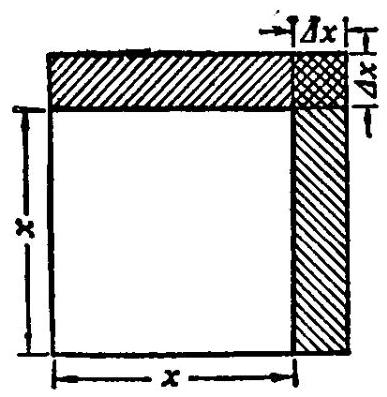
\includegraphics[max width=0.4\textwidth]{images/01912c18-5c3f-733d-b775-749ba9897a9d_110_353714.jpg}
\end{center}

图 2-4

设有边长为 \(x\) 的正方形铁片,加热后边长增加了 \({\Delta x}\) (图 2-4), 求铁片的面积约增加多少.

加热前铁片的面积为 \(y = f\left( x\right) = {x}^{2}\) ,当边长增加了 \({\Delta x}\) ,铁片面积的增加量就是函数 \(f\left( x\right)\) 的改变量

\[
{\Delta y} = {\left( x + \Delta x\right) }^{2} - {x}^{2}
\]

\[
= {x}^{2} + {2x} \cdot {\Delta x} + {\left( \Delta x\right) }^{2} - {x}^{2}
\]

\[
= {2x} \cdot {\Delta x} + {\left( \Delta x\right) }^{2}\text{.} \tag{1}
\]

\({\Delta y}\) 由两部分组成: 一部分是 \({\Delta x}\) 的线性函数 \({2x} \cdot {\Delta x}\) (图 2-4 中单线阴影部分的面积); 另一部分是 \({\left( \Delta x\right) }^{2}\) (图 2-4 中双线阴影部分的面积).

如果以 \({2x} \cdot {\Delta x}\) 作为 \({\Delta y}\) 的近似值,其误差为

\[
{\Delta y} - {2x} \cdot {\Delta x} = {\left( \Delta x\right) }^{2}.
\]

这个误差 \({\left( \Delta x\right) }^{2}\) 显然随着 \(\left| {\Delta x}\right|\) (在这个实际问题中, \({\Delta x} > 0\) ,可以去掉绝对值符号)的减小而减小,而且, \({\left( \Delta x\right) }^{2}\) 要比 \(\left| {\Delta x}\right|\) 减小得更快些 (例如, \(\left| {\Delta x}\right|\) 从 0.1 减小到 0.01, \({\left( \Delta x\right) }^{2}\) 就相应地从 0.01 减小到 0.0001 ),当 \(\left| {\Delta x}\right|\) 很小时, \({\left( \Delta x\right) }^{2}\) 比 \(\left| {\Delta x}\right|\) 要小得多 (例如 \(\left| {\Delta x}\right| = {10}^{-5}\) ,则 \({\left( \Delta x\right) }^{2} = {10}^{-{10}}\) ). 因此式子 \({\Delta y} = {2x} \cdot {\Delta x} + {\left( \Delta x\right) }^{2}\) 右边的两项中,第一项 \({2x} \cdot {\Delta x}\) 是主要部分. 当 \(\left| {\Delta x}\right|\) 很小时,可认为铁片面积增加量

\[
{\Delta y} \approx {2x} \cdot {\Delta x}.
\]

这样我们可以用计算 \({2x\Delta x}\) 来代替计算 \(y = {x}^{2}\) 的改变量 \({\Delta y}\) ,这比计算 \({\Delta y}\) 来得简便,且有一定的精确度.

由 \({2x} = {\left( {x}^{2}\right) }^{\prime } = {f}^{\prime }\left( x\right)\) ,于是在上例中有

\[
{\Delta y} \approx {f}^{\prime }\left( x\right) \cdot {\Delta x}.
\]

\[
\left( {1}^{\prime }\right)
\]

一般地,设函数 \(y = f\left( x\right)\) 在点 \(x\) 处可导,则 \(y = f\left( x\right)\) 在点 \(x\) 处的导数 \({f}^{\prime }\left( x\right)\) 与自变量的改变量 \({\Delta x}\) 的积叫做函数 \(y\) \(= f\left( x\right)\) 在点 \(x\) 处关于改变量 \({\Delta x}\) 的微分,简称函数 \(y\) 的微分, 记作 \({dy}\) ,即

\[
{dy} = {f}^{\prime }\left( x\right) {\Delta x}. \tag{2}
\]

因此,在 \(y = {x}^{2}\) 时,

\[
{\Delta y} \approx {f}^{\prime }\left( x\right) {\Delta x} = {dy}.
\]

\[
\left( {2}^{\prime }\right)
\]

即函数的改变量 \({\Delta y}\) 可用它的微分近似地表示出来. 对于一般的可导函数也有同样的结果, 我们就不证了. 这样, 就可以把计算较为复杂的 \({\Delta y}\) 转化为计算 \({dy}\) ,即只要求出导数值 \({f}^{\prime }\left( x\right)\) 再乘以 \({\Delta x}\) 就行了.

例 半径为 \({10}\mathrm{\;{cm}}\) 的金属圆片加热后,半径伸长了 \({0.05}\mathrm{\;{cm}}\) ,求此时刻面积的微分 \({dA}\) 与 \({\Delta A} - {dA}\) 的值.

解: 以 \(A\) 表示圆片的面积, \(r\) 表示圆片的半径,则

\[
A = \pi {r}^{2}.
\]

根据题意,取 \(r = {10},{\Delta r} = {0.05}\) . 这时,

\[
{dA} = {2\pi r} \cdot {\Delta r}
\]

\[
= {2\pi } \times {10} \times {0.05} = \pi \left( {\mathrm{{cm}}}^{2}\right) \text{.}
\]

\(\because \;{\Delta A} = \pi {\left( r + \Delta r\right) }^{2} - \pi {r}^{2} = {2\pi r} \cdot {\Delta r} + \pi {\left( \Delta r\right) }^{2},\)

\[
\therefore \;{\Delta A} - {dA} = {2\pi r} \cdot {\Delta r} + \pi {\left( \Delta r\right) }^{2} - {2\pi r} \cdot {\Delta r} = \pi {\left( \Delta r\right) }^{2}
\]

\[
= \pi {\left( {0.05}\right) }^{2}
\]

\[
= {0.0025\pi }\left( {\mathrm{{cm}}}^{2}\right) \text{.}
\]

答: 面积的微分 \({dA}\) 为 \(\pi {\mathrm{{cm}}}^{2},{\Delta A} - {dA}\) 为 \({0.0025\pi }{\mathrm{{cm}}}^{2}\) .

在本例中, 如果“加热”改为“冷却”, “伸长”改为“缩短”, 这时,可取 \(r = {10},{\Delta r} = - {0.05}\) ,于是 \({dA}\) 为 \(- \pi {\mathrm{{cm}}}^{2},{\Delta A} - {dA}\) 为 \(- {0.0025\pi }{\mathrm{{cm}}}^{2}\) .

通常把自变量的改变量 \({\Delta x}\) 记作 \({dx}\) ,即 \({dx} = {\Delta x}\) ,称为自变量的微分. 于是函数 \(y = f\left( x\right)\) 的微分也可以写成

\[
{dy} = {f}^{\prime }\left( x\right) {dx}. \tag{3}
\]

在 (3) 式两边同时除以 \({dx}\) ,得到 \({f}^{\prime }\left( x\right) = \frac{dy}{dx}\) . 这样,函数 \(y = f\left( x\right)\) 的导数 \({f}^{\prime }\left( x\right)\) 就等于函数的微分 \({dy}\) 与自变量的微分 \({dx}\) 的商,所以导数也叫做微商. 今后,我们也采用记号 \(\frac{dy}{dx}\) 来表示函数 \(y = f\left( x\right)\) 的导数 \({f}^{\prime }\left( x\right)\) ,即

\[
\frac{dy}{dx} = {f}^{\prime }\left( x\right) = {y}_{x}^{\prime } = \mathop{\lim }\limits_{{{\Delta x} \rightarrow 0}}\frac{\Delta y}{\Delta x}.
\]

我们还采用记号 \(\frac{{d}^{2}y}{d{x}^{2}}\) 来表示二阶导数 \({f}^{\prime \prime }\left( x\right) ,\cdots \cdots\) ,采用记号 \(\frac{{d}^{n}y}{d{x}^{n}}\) 来表示 \(n\) 阶导数 \({f}^{\left( n\right) }\left( x\right)\) 等等.

下面我们来说明函数的微分的几何意义.

设函数 \(y = f\left( x\right)\) 在点 \(x\) 处可导,如图 2-5,在 \(y = f\left( x\right)\) 所表示的曲线上取点 \(P\left( {x,y}\right)\) 及它邻近的点 \({P}^{\prime }\left( {x + {\Delta x},y + {\Delta y}}\right)\) ,过点 \(P\) 及 \({P}^{\prime }\) 作 \({MP}\) 及 \({M}^{\prime }{P}^{\prime }\) 垂直于 \(x\) 轴,分别交 \(x\) 轴于点 \(M\) 及 \({M}^{\prime }\) ,过点 \(P\) 作平行于 \(x\) 轴的直线交 \({M}^{\prime }{P}^{\prime }\) 于点 \(N\) ,又作曲线 \(y = f\left( x\right)\) 在点 \(P\) 处的切线,交 \({M}^{\prime }{P}^{\prime }\) 于点 \(T\) ,则

\[
{PN} = {\Delta x},\;N{P}^{\prime } = {\Delta y},
\]

\[
{NT} = {f}^{\prime }\left( x\right) {\Delta x} = {dy}.
\]

\begin{center}
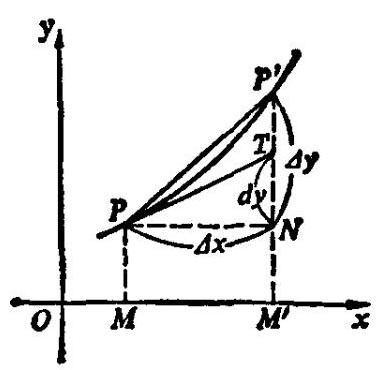
\includegraphics[max width=0.4\textwidth]{images/01912c18-5c3f-733d-b775-749ba9897a9d_113_880246.jpg}
\end{center}

图 2-5

所以,当自变量的改变量为 \({\Delta x}\) 时, \({\Delta y}\) 就是曲线的纵坐标的改变量, \({dy}\) 就是切线的纵坐标的改变量,这就是函数的微分的几何意义. \({\Delta y}\) 与 \({dy}\) 的差的绝对值在图形上是 \(\left| {T{P}^{\prime }}\right|\) ,一般地,它是随着 \(\left| {\Delta x}\right|\) 减小而减小,而且要比 \(\left| {\Delta x}\right|\) 减小得更快些. 所以,当 \(\left| {\Delta x}\right|\) 很小时, \({\Delta y} \approx {dy}\) . 这时,可以用切线的纵坐标的改变量来代替曲线的纵坐标的改变量. 用 \({dy}\) 近似表示 \({\Delta y}\) , 相当于在点 \(P\left( {x,y}\right)\) 附近用切线段 \({PT}\) 近似地代替曲线段 \(P{P}^{\prime }\) . 这种在一定条件下以直代曲的方法是微分和积分中常用的典型方法.

\section{微分的运算}

由微分的表示式 \({dy} = {f}^{\prime }\left( x\right) {dx}\) 知道,已知函数求微分时, 只要求出函数的导数再乘以自变量的微分. 计算微分或导数的方法也叫做微分法.

例 1 求 \(y = \sin x\) 的微分.

\[
\text{解:}\;{dy} = {\left( \sin x\right) }^{\prime }{dx} = \cos {xdx}\text{.}
\]

例 2 求 \(y = \operatorname{arctg}x\) 的微分.

解: \(\;{dy} = {\left( \operatorname{arctg}x\right) }^{\prime }{dx} = \frac{dx}{1 + {x}^{2}}\) .

根据导数的基本公式,利用 \({dy} = {f}^{\prime }\left( x\right) {dx}\) 我们就可求出相应的微分公式.

\section*{微分公式表}

(1) \(d\left( C\right) = 0\) ; (7) \(d\left( {\operatorname{tg}x}\right) = {\sec }^{2}{xdx}\) ;

(2) \(d\left( {x}^{\alpha }\right) = \alpha {x}^{\alpha - 1}{dx}\) ; (8) \(d\left( {\operatorname{ctg}x}\right) = - {\csc }^{2}{xdx}\) ;

(3) \(d\left( {{\log }_{a}x}\right) = \frac{dx}{x\ln a}\) ; (9) \(d\left( {\arcsin x}\right) = \frac{dx}{\sqrt{1 - {x}^{2}}}\) ;

\(d\left( {\ln x}\right) = \frac{dx}{x}\) (10) \(d\left( {\arccos x}\right) = - \frac{dx}{\sqrt{1 - {x}^{2}}}\) ;

(4) \(d\left( {a}^{x}\right) = {a}^{x}\ln {adx}\) ; (11) \(d\left( {\operatorname{arctg}x}\right) = \frac{dx}{1 + {x}^{2}}\) ;

\[
d\left( {e}^{x}\right) = {e}^{x}{dx}
\]

(5) \(d\left( {\sin x}\right) = \cos {xdx}\) ; (12) \(d\left( {\operatorname{arcctg}x}\right) = - \frac{dx}{1 + {x}^{2}}\) .

(6) \(d\left( {\cos x}\right) = - \sin {xdx}\) ;

同样, 由求导数的四则运算法则, 可以得出相应的求微分的四则运算法则:

(1) \(d\left( {u \pm v}\right) = {du} \pm {dv}\) .

(2) \(d\left( {uv}\right) = {udv} + {vdu}\) .

请同学们自己证明(1)、(2)。

(3) \(d\left( \frac{u}{v}\right) = \frac{{vdu} - {udv}}{{v}^{2}}\) .

证明: \(d\left( \frac{u}{v}\right) = {\left( \frac{u}{v}\right) }^{\prime }{dx} = \frac{v{u}^{\prime } - u{v}^{\prime }}{{v}^{2}}{dx}\)

\[
= \frac{v\left( {{u}^{\prime }{dx}}\right) - u\left( {{v}^{\prime }{dx}}\right) }{{v}^{2}} = \frac{{vdu} - {udv}}{{v}^{2}}.
\]

例 3 求 \(y = {e}^{ax}\sin {bx}\) 的微分.

\[
\text{解:}\;{dy} = {e}^{ax}d\left( {\sin {bx}}\right) + \sin {bxd}\left( {e}^{ax}\right)
\]

\[
= {e}^{ax} \cdot b\cos {bxdx} + \sin {bx} \cdot a{e}^{ax}{dx}
\]

\[
= {e}^{ax}\left( {b\cos {bx} + a\sin {bx}}\right) {dx}\text{.}
\]

\begin{problemset}[练习]

\item 对于函数 \(y = {x}^{3} - x\) 和下列的 \({\Delta x}\) 的值,求点 \(x = 2\) 处的 \({\Delta y}\) 和 \({dy}\) :

(1) \({\Delta x} = 1\) ; (2) \({\Delta x} = {0.1}\) ;

(3) \({\Delta x} = {0.01}\) ; (4) \({\Delta x} = {0.001}\) .

\item 求下列函数的微分:

(1) \(y = 3{x}^{4} - 5{x}^{2} + 1\) ; (2) \(y = \left( {2{x}^{2} - 3}\right) \left( {{3x} + 4}\right)\) ;

(3) \(y = \frac{1 - {x}^{2}}{1 + {x}^{2}}\) (4) \(y = \frac{1}{3}{\operatorname{tg}}^{3}\theta + \operatorname{tg}\theta\) ;

(5) \(y = {e}^{2x}\sin {5x}\) ; (6) \(y = \operatorname{arctg}\left( {\ln x}\right)\) .

\item 函数 \(y = f\left( x\right)\) 的微分 \({dy}\) 依赖于哪两个量?

\item 边长 \(4\mathrm{\;{cm}}\) 的正方形铁皮,在加热中边长增加了 \({0.001}\mathrm{\;{cm}}\) , 求此时刻面积的微分 \({dS}\) 与 \({\Delta S} - {dS}\) 的值.

\item 半径 \(R\) 为 \({10}\mathrm{\;{cm}}\) 的球,在冷却中 \(R\) 缩短了 \({0.001}\mathrm{\;{cm}}\) ,求此

时刻体积的微分 \({dV}\) 与 \({\Delta V} - {dV}\) 的值.

\item 求证 \(\frac{d\left( {\sin x}\right) }{d\left( {\cos x}\right) } = - \operatorname{ctg}x\) .

\end{problemset}

\section{近似计算}

我们知道,当 \(\left| {\Delta x}\right|\) 很小时,可以用微分 \({dy}\) 近似代替函数 \(y = f\left( x\right)\) 的改变量 \({\Delta y}\) . 由于在点 \({x}_{0}\) 处,

\[
{dy} = {f}^{\prime }\left( {x}_{0}\right) {\Delta x}
\]

\[
{\Delta y} = f\left( {{x}_{0} + {\Delta x}}\right) - f\left( {x}_{0}\right) ,
\]

于是有

\[
f\left( {{x}_{0} + {\Delta x}}\right) - f\left( {x}_{0}\right) \approx {f}^{\prime }\left( {x}_{0}\right) {\Delta x},
\]

改写一下, 得

\[
f\left( {{x}_{0} + {\Delta x}}\right) \approx f\left( {x}_{0}\right) + {f}^{\prime }\left( {x}_{0}\right) {\Delta x}. \tag{1}
\]

如果把 \({x}_{0} + {\Delta x}\) 记作 \(x\) ,那么 \({\Delta x} = x - {x}_{0}\) ,于是 (1)式也可写成

\[
f\left( x\right) \approx f\left( {x}_{0}\right) + {f}^{\prime }\left( {x}_{0}\right) \left( {x - {x}_{0}}\right) . \tag{2}
\]

如果我们要求函数 \(y = f\left( x\right)\) 在某一点 \(x\) 处的值,但这点的值不易求出,而在 \(x\) 附近的 \({x}_{0}\) 处, \(f\left( {x}_{0}\right)\) 和 \({f}^{\prime }\left( {x}_{0}\right)\) 的值都容易求出,这时,我们可以利用 (2) 式 (或 (1) 式) 来求 \(f\left( x\right)\) 的近似值. 要注意的是这里要求 \(\left| {x - {x}_{0}}\right| = \left| {\Delta x}\right|\) 很小, \(\left| {x - {x}_{0}}\right|\) 越小, 近似程度越好.

例 1 不查表,求 \(\sin {46}^{ \circ }\) 的近似值.

解: 令 \(y = \sin x\) ,由 (2) 式,

\[
\sin x \approx \sin {x}_{0} + \cos {x}_{0} \cdot \left( {x - {x}_{0}}\right) .
\]

因为 \({46}^{ \circ } = {45}^{ \circ } + {1}^{ \circ } = \left( {\frac{\pi }{4} + \frac{\pi }{180}}\right)\) 弧度,

取 \({x}_{0} = \frac{\pi }{4},x = \frac{\pi }{4} + \frac{\pi }{180}\) ,于是 \(x - {x}_{0} = \frac{\pi }{180}\) ,代入上式得

\[
\sin {46}^{ \circ } = \sin \left( {\frac{\pi }{4} + \frac{\pi }{180}}\right)
\]

\[
\approx \sin \frac{\pi }{4} + \cos \frac{\pi }{4} \cdot \frac{\pi }{180}
\]

\[
= \frac{\sqrt{2}}{2} + \frac{\sqrt{2}}{2} \cdot \frac{\pi }{180}
\]

\[
\approx {0.7071} + {0.0123}
\]

\[
= {0.7194}\text{.}
\]

如果把 (2) 式中的 \(x\) 看成变量,(2) 式右边就是 \(x\) 的一次函数. 也就是说,当 \(\left| {x - {x}_{0}}\right|\) 很小时,可以用一次函数 \(y = f\left( {x}_{0}\right)\) \(+ {f}^{\prime }\left( {x}_{0}\right) \left( {x - {x}_{0}}\right)\) 来近似表示函数 \(y = f\left( x\right)\) ; 从几何上看,也就是在点 \(\left( {{x}_{0},{y}_{0}}\right)\) 附近,用曲线 \(y = f\left( x\right)\) 上点 \(\left( {{x}_{0},{y}_{0}}\right)\) 处的切线 \(y - {y}_{0} = {f}^{\prime }\left( {x}_{0}\right) \left( {x - {x}_{0}}\right)\) 来近似表示曲线 \(y = f\left( x\right)\) .

当 \({x}_{0} = 0\) 时,(2)式变为

\[
f\left( x\right) \approx f\left( 0\right) + {f}^{\prime }\left( 0\right) x. \tag{3}
\]

利用(3)式,当 \(\left| x\right|\) 充分小时,可以导出常用的一些近似公式:

\[
\sqrt{1 + x} \approx 1 + \frac{x}{2}
\]

\[
\left( {1}^{ \circ }\right)
\]

\[
\ln \left( {1 + x}\right) \approx x
\]

\[
\left( {2}^{ \circ }\right)
\]

\[
{e}^{x} \approx 1 + x
\]

\[
\left( {3}^{ \circ }\right)
\]

\[
\operatorname{tg}x \approx x\text{.}
\]

\[
\left( {4}^{ \circ }\right)
\]

下面写出这些近似公式的导出过程.

\(\left( {1}^{ \circ }\right)\) 取 \(f\left( x\right) = \sqrt{1 + x}\) ,则

\[
{f}^{\prime }\left( x\right) = \frac{1}{2\sqrt{1 + x}}
\]

于是

\[
f\left( 0\right) = 1,{f}^{\prime }\left( 0\right) = \frac{1}{2}.
\]

由 \(\left( 3\right)\) 式,得

\[
\sqrt{1 + x} = f\left( x\right) \approx f\left( 0\right) + {f}^{\prime }\left( 0\right) x
\]

\[
= 1 + \frac{x}{2}
\]

即

\[
\sqrt{1 + x} \approx 1 + \frac{x}{2}
\]

\(\left( {2}^{ \circ }\right)\) 取 \(f\left( x\right) = \ln \left( {1 + x}\right)\) ,则

\[
{f}^{\prime }\left( x\right) = \frac{1}{1 + x}
\]

于是

\[
f\left( 0\right) = 0,{f}^{\prime }\left( 0\right) = 1\text{. }
\]

由 \(\left( 3\right)\) 式,得

\[
\ln \left( {1 + x}\right) \approx x\text{. }
\]

\begin{itemize}
\item \(\left( {3}^{ \circ }\right)\) 取 \(f\left( x\right) = {e}^{x}\) ,则
\end{itemize}

\[
{f}^{\prime }\left( x\right) = {e}^{x}
\]

于是

\[
f\left( 0\right) = 1,{f}^{\prime }\left( 0\right) = 1\text{. }
\]

由 \(\left( 3\right)\) 式,得

\[
{e}^{x} \approx 1 + x\text{. }
\]

\(\left( {4}^{ \circ }\right)\) 取 \(f\left( x\right) = \operatorname{tg}x\) ,则

\[
{f}^{\prime }\left( x\right) = {\sec }^{2}x
\]

于是

\[
f\left( 0\right) = 0,{f}^{\prime }\left( 0\right) = 1\text{. }
\]

由 \(\left( 3\right)\) 式,得

\[
\operatorname{tg}x \approx x\text{.}
\]

例 2 根据导出的近似公式, 求下列各式的近似值:

(1) \(\sqrt{4.01},\sqrt{8.997}\) ; (2) \(\ln {1.002},\ln {0.998}\) ;

(3) \({e}^{0.01},{e}^{-{0.02}}\) .

解: (1) \(\sqrt{4.01} = \sqrt{4\left( {1 + \frac{0.01}{4}}\right) } = 2\sqrt{1 + \frac{0.01}{4}}\) . 利用公式 \(\left( {1}^{ \circ }\right)\) ,取 \(x = \frac{0.01}{4}\) ,得

\[
\sqrt{4.01} \approx 2\left( {1 + \frac{0.01}{2 \times 4}}\right) = {2.0025}.
\]

\[
\sqrt{8.997} = \sqrt{9\left( {1 - \frac{0.003}{9}}\right) } = 3\sqrt{1 - \frac{0.003}{9}}\text{. 利用公式}\left( {1}^{ \circ }\right) \text{,}
\]

取 \(x = - \frac{0.003}{9}\) ,得

\[
\sqrt{8.997} \approx 3\left( {1 - \frac{0.003}{2 \times 9}}\right) = {2.9995}.
\]

(2)利用公式 \(\left( {2}^{ \circ }\right)\) . 取 \(x = {0.002}\) ,得

\[
\ln {1.002} = \ln \left( {1 + {0.002}}\right) \approx {0.002}\text{.}
\]

取 \(x = - {0.002}\) ,得

\[
\ln {0.998} = \ln \left( {1 - {0.002}}\right) \approx - {0.002}.
\]

(3)利用公式 \(\left( {3}^{ \circ }\right)\) ,取 \(x = {0.01}\) ,得

\[
{e}^{0.01} \approx 1 + {0.01} = {1.01}.
\]

取 \(x = - {0.02}\) ,得

\[
{e}^{-{0.02}} \approx 1 - {0.02} = {0.98}.
\]

例 3 如图 2-6, 加工锥形工件时, 已知工件两头直径分

别为 \({d}_{1},{d}_{2}\) ,长度为 \(l\) ,当斜角 \(\alpha\) 很小时,导出近似关系式:

\[
\alpha \approx {28.6}^{ \circ } \times \frac{{d}_{1} - {d}_{2}}{l}.
\]

\begin{center}
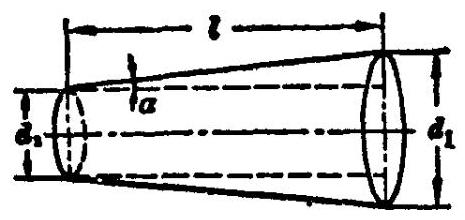
\includegraphics[max width=0.5\textwidth]{images/01912c18-5c3f-733d-b775-749ba9897a9d_120_883650.jpg}
\end{center}

图 2-6

解: 由图,

\[
\operatorname{tg}\alpha = \frac{{d}_{1} - {d}_{2}}{2l}.
\]

当 \(\alpha\) 很小时,根据公式 \(\left( {4}^{ \circ }\right)\) ,

\[
\operatorname{tg}\alpha \approx \alpha ,
\]

\[
\therefore \;\alpha \approx \frac{{d}_{1} - {d}_{2}}{2l}\text{. }
\]

又

\[
\text{1 弧度} = {\left( \frac{180}{\pi }\right) }^{ \circ } \approx {57.3}^{ \circ }\text{,}
\]

\(\therefore \;\alpha \approx {57.3}^{ \circ } \times \frac{{d}_{1} - {d}_{2}}{2l} \approx {28.6}^{ \circ } \times \frac{{d}_{1} - {d}_{2}}{l}\) .

\begin{problemset}[练习]

\item 在例 1 中, \(x - {x}_{0} = \frac{\pi }{180}\) ,是用弧度为单位,为什么? 如果用度为单位,取 \(x - {x}_{0} = 1\) ,得出的结果对不对?

\item 已知 \(\ln {10} = {2.3026}\) ,利用 \(f\left( x\right) \approx f\left( {x}_{0}\right) + {f}^{\prime }\left( {x}_{0}\right) \left( {x - {x}_{0}}\right)\) 求 \(\ln {10.012}\) 的近似值.

\item 当 \(\left| x\right|\) 很小时,导出下列近似公式:

(1) \(\sqrt[n]{1 + x} \approx 1 + \frac{x}{n}\)\(\left( {5}^{ \circ }\right)\)

(2) \(\sin x \approx x\) .\(\left( {6}^{ \circ }\right)\)

\item 计算下列各式的近似值:

(1) \(\sqrt[5]{1.02}\) ; (2) \(\sqrt[3]{0.998}\) ;

(3) \({e}^{-{0.1}}\) (4) \(\operatorname{tg}{0.01}\) ;

(5) \(\sin {0.1}^{ \circ }\) ; (6) \(\ln {1.0021}\) .

\end{problemset}

\begin{problemset}[习 题 八]

\item (1) 在下列图形中,标出相应的 \({\Delta y}\) 和 \({dy}\) 。

\begin{center}
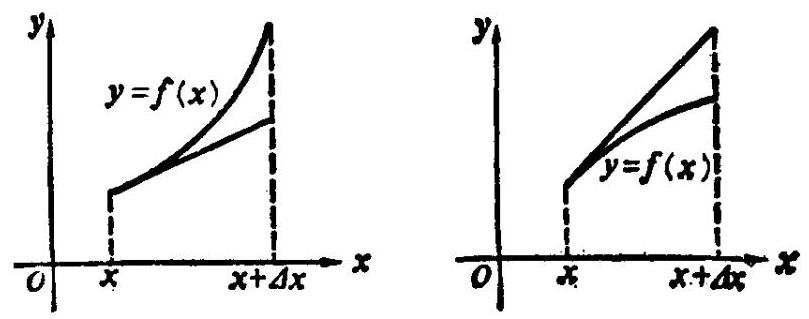
\includegraphics[max width=0.8\textwidth]{images/01912c18-5c3f-733d-b775-749ba9897a9d_121_587843.jpg}
\end{center}

(第 1 (1) 题)

(2)自变量 \(x\) 的微分 \({dx}\) 是否一定为正? 当 \({dx}\) 为正时, 函数 \(y = f\left( x\right)\) 的微分 \({dy}\) 是否一定为正?

\item 求下列函数的微分:

(1) \(y = a{x}^{3} + b{x}^{2} + {cx} + d\) ; (2) \(y = {\left( {a}^{2} - {x}^{2}\right) }^{5}\) ;

(3) \(y = \frac{\left( {x - 1}\right) \left( {x - 2}\right) }{\left( {x + 1}\right) \left( {x + 2}\right) }\) (4) \(r = \left( {1 + {\theta }^{2}}\right) \operatorname{tg}\theta\) ;

(5) \(y = {e}^{-x}\ln x\) ;

(6) \(y = \arcsin {3x} + {3x}\sqrt{1 - 9{x}^{2}}\) ;

(7) \(y = \frac{{x}^{2n}}{{\left( 1 + {x}^{2}\right) }^{n}}\) ; (8) \(y = t - \frac{{e}^{t} - {e}^{-t}}{{e}^{t} + {e}^{-t}}\) .

\item 求函数 \(y = {x}^{3}\) 在自变量的值由 \(x = 1\) 变为 \(x + {\Delta x} = {1.01}\) 时的改变量 \({\Delta y}\) 及 \({dy}\) . 用 \({dy}\) 来近似地代替 \({\Delta y}\) 的误差是多少?

\item 某运动方程为

\[
s = 4{t}^{2}
\]

其中 \(t\) 的单位是秒, \(s\) 的单位是米,求 \(t = 2\) 秒, \({\Delta t} = {0.001}\) 秒时路程的改变量 \({\Delta s}\) 及路程的微分 \({ds}\) ,并加以比较.

\item 一金属圆管的内半径为 \({10}\mathrm{\;{cm}}\) ,厚度为 \({0.05}\mathrm{\;{cm}}\) ,求圆管的横截面积的近似值.

\item 球壳的外直径是 \({30}\mathrm{\;{cm}}\) ,厚度是 \({0.1}\mathrm{\;{cm}}\) ,求球壳体积的近似值.

\item 要在直径为 \({50}\mathrm{\;{cm}}\) 的半球面形锅的内侧镀锌 (锌的比重为 \(7\mathrm{\;g}/{\mathrm{{cm}}}^{3}\) ),镀层厚 \({0.005}\mathrm{\;{cm}}\) ,约需用锌多少克?

\item 计算下列各式的近似值:

(1) \(\sqrt{9.01}\) ; (2) \(\sqrt{15.98}\) ;

(3) \(\sqrt[3]{1.004}\) (4) \(\sqrt[3]{0.982}\) ;

(5) \({e}^{-{0.03}}\) (6) \({\left( {1.002}\right) }^{5}\) ;

(7) \(\ln {1.01}\) ; (8) \(\ln {0.97}\) ;

(9) \(\sin {0.016}\) ; (10) \(\operatorname{tg}{0.025}\) ;

\item 当 \(\left| x\right|\) 很小时,导出近似公式:

\[
{\left( 1 + x\right) }^{\alpha } \approx 1 + {\alpha x}\;\left( {\alpha \text{ 为实数 }}\right) ,
\]

\[
\left( {7}^{ \circ }\right)
\]

并求 \({1.001}^{0.13}\) 的近似值.

\end{problemset}

\chapter*{小 结}
\markboth{小 结}{小 结}

一、本章主要内容是导数和微分的概念、求导数和求微分的方法以及微分在近似计算上的某些应用.

二、导数概念是微积分学的基本概念之一. 函数 \(y = f\left( x\right)\)

的导数 \({f}^{\prime }\left( x\right)\) ,就是函数的改变量 \({\Delta y}\) 与自变量的改变量 \({\Delta x}\) 的比 \(\frac{\Delta y}{\Delta x}\) 当 \({\Delta x} \rightarrow 0\) 时的极限,即

\[
{f}^{\prime }\left( x\right) = \mathop{\lim }\limits_{{{\Delta x} \rightarrow 0}}\frac{\Delta y}{\Delta x} = \mathop{\lim }\limits_{{{\Delta x} \rightarrow 0}}\frac{f\left( {x + {\Delta x}}\right) - f\left( x\right) }{\Delta x},
\]

它表示在点 \(x\) 处函数 \(y\) 对自变量的变化率,它的几何意义是曲线 \(y = f\left( x\right)\) 在点 \(\left( {x,f\left( x\right) }\right)\) 处的切线的斜率.

如果 \({f}^{\prime }\left( {x}_{0}\right)\) 存在,曲线 \(y = f\left( x\right)\) 上点 \(\left( {{x}_{0},{y}_{0}}\right)\) 处的切线的方程为

\[
y - {y}_{0} = {f}^{\prime }\left( {x}_{0}\right) \left( {x - {x}_{0}}\right)
\]

法线的方程 (当 \({f}^{\prime }\left( {x}_{0}\right) \neq 0\) 时) 为

\[
y - {y}_{0} = - \frac{1}{{f}^{\prime }\left( {x}_{0}\right) }\left( {x - {x}_{0}}\right) .
\]

三、函数 \(y = f\left( x\right)\) 的微分 \({dy}\) 就是函数的导数 \({f}^{\prime }\left( x\right)\) 与自变量的微分 \({dx}\left( {{dx} = {\Delta x} \neq 0}\right)\) 的积,即

\[
{dy} = {f}^{\prime }\left( x\right) {dx}.
\]

求函数 \(y = f\left( x\right)\) 的导数 \({f}^{\prime }\left( x\right)\) 与求函数的微分 \({f}^{\prime }\left( x\right) {dx}\) 是互通的, 即

\[
\frac{dy}{dx} = {f}^{\prime }\left( x\right) \Leftrightarrow {dy} = {f}^{\prime }\left( x\right) {dx},
\]

所以导数也叫做微商.

四、求函数的导数或微分的方法叫做微分法. 根据定义求导数是最基本的方法. 对初等函数来说, 只要根据定义先求得一些基本初等函数的导数, 再利用求导数 (或微分) 的四则运算法则以及复合函数、反函数的求导 (或微分) 法则, 就可以求出任一初等函数的导数 (或微分). 这里, 复合函数的求导法则特别重要, 应切实掌握.

五、根据微分的定义及其几何意义, 有下列近似公式:

\[
{\Delta y} \approx {f}^{\prime }\left( {x}_{0}\right) {\Delta x}\;\left( {\left| {\Delta x}\right| \text{ 很小 }}\right) ,
\]

\[
f\left( x\right) \approx f\left( {x}_{0}\right) + {f}^{\prime }\left( {x}_{0}\right) \left( {x - {x}_{0}}\right) \;\left( {\left| {x - {x}_{0}}\right| \text{ 很小 }}\right) .
\]

利用这些公式, 可以求出函数的改变量或在某一点处的函数值的近似值.

特别当 \({x}_{0} = 0\) 时,有

\[
f\left( x\right) \approx f\left( 0\right) + {f}^{\prime }\left( 0\right) x\;\left( {\left| x\right| \text{ 很小 }}\right) .
\]

由此可以导出一些常用的近似公式, 从而使实际问题中的一些计算大为简化.

\chapter*{复习参考题二}
\markboth{复习参考题二}{复习参考题二}

\section*{\(A\) 组}

1. (1) 在导数的定义中, \(\mathop{\lim }\limits_{{{\Delta x} \rightarrow 0}}\frac{\Delta y}{\Delta x}\) 的 \({\Delta x}\) 是正的还是负的? 还

是可正可负? \(\mathop{\lim }\limits_{{{\Delta x} \rightarrow 0 + }}\frac{\Delta y}{\Delta x}\) 的 \({\Delta x}\) 呢? \(\mathop{\lim }\limits_{{{\Delta x} \rightarrow 0}}\frac{\Delta y}{\Delta x}\) 的 \({\Delta x}\) 呢?

\(\mathop{\lim }\limits_{{{\Delta x} \rightarrow 0}}\frac{\Delta y}{\Delta x}\) 与 \(\mathop{\lim }\limits_{{{\Delta x} \rightarrow 0 + }}\frac{\Delta y}{\Delta x}\) 及 \(\mathop{\lim }\limits_{{{\Delta x} \rightarrow 0 - }}\frac{\Delta y}{\Delta x}\) 之间有什么关系?

(2) \({f}^{\prime }\left( x\right)\) 和 \({f}^{\prime }\left( {x}_{0}\right)\) 有什么不同? \({f}^{\prime }\left( {x}_{0}\right)\) 与 \({\left\lbrack f\left( {x}_{0}\right) \right\rbrack }^{\prime }\) 有什么不同?

2. 一质点沿 \({OA}\) 轴运动,在时刻 \(t\) (秒)时,质点的位置 \(s = {6t} - {t}^{2}\) (米).

(1)求 \(t = 0,2,3,6,7\) 时质点的位置. 当 8 取负值时意

味着什么?

(2)求速度 \(v\left( {\text{米}/\text{秒}}\right)\) 的表示式,并求 \(t = 0,2,3,6,7\) 时的 \(v\) 值. \(v\) 值为负时意味着什么?

(3)什么时刻以后, 质点改变运动的方向?

3. 在受到制动后的 \(t\) 秒钟内飞轮转过的角度(弧度)由函数 \(\varphi \left( t\right) = {4t} - {0.3}{t}^{2}\) 给出,求:

(1) \(t = 2\) (秒) 时,飞轮转过的角度;

(2)飞轮停止旋转的时刻.

4. 假设 1 公斤的铁从 \({0}^{ \circ }\mathrm{C}\) 加热到 \({t}^{ \circ }\mathrm{C}\left( {0 \leq t \leq {200}}\right)\) 时,所吸收的热量 \(Q\left( \text{千卡 }\right)\) 由公式 \(Q\left( t\right) = {0.1053t} + {0.000071}{t}^{2}\) 确定,求 \(t = {50}\) 时铁的比热 \(C\) .

(提示: 比热 \(C = {Q}^{\prime }\left( t\right)\) 千卡/公斤. 度. )

5. 已知抛物线 \(y = {x}^{2} - 4\) 及直线 \(y = x + 2\) ,求直线与抛物线在交点处的切线的交角.

6. 已知两曲线 \(y = {x}^{2} - 1\) 与 \(y = 1 - {x}^{3}\) .

(1)这两曲线在横坐标为 \({x}_{0}\) 的点处的切线互相平行,求 \({x}_{0}\) 的值;

(2)这两曲线在横坐标为 \({x}_{1}\) 的点处的切线互相垂直,求 \({x}_{1}\) 的值.

7. 按定义求 \(y = \operatorname{tg}x\) 的导数.

8. 求下列函数的导数:

(1) \(y = \left( {{x}^{2} - 1}\right) \left( {{x}^{2} - 3}\right) \left( {{x}^{2} - 5}\right)\) ; (2) \(y = \frac{{x}^{2}}{{\left( {x}^{2} - 1\right) }^{3}}\) ;

(3) \(y = \frac{\sin {2x}}{1 + x}\) (4) \(y = \frac{\sec x}{1 + \operatorname{tg}x}\)

(5) \(y = {\sin }^{4}{3x}{\cos }^{3}{4x}\) ; (6) \(y = 2\left( {{e}^{\frac{x}{2}} + {e}^{-\frac{x}{2}}}\right)\) ;

(7) \(y = x\arcsin \frac{x}{2} + \sqrt{4 - {x}^{2}}\) ; (8) \(y = {a}^{{2x} + 1}\) ;

(9) \(y = \arccos \frac{x - 3}{3} - 2\sqrt{\frac{6 - x}{x}}\)

(10) \(y = \frac{x\ln x}{x + 1} - \ln \left( {x + 1}\right)\) ; (11) \(y = \lg \left( {{x}^{2} + x + 1}\right)\) ;

(12) \(y = \ln \left( {{\cos }^{2}x}\right) + {2x}\operatorname{tg}x - {x}^{2}\) .

9. 求下列函数的导数:

(1) \(y = \frac{x - a}{\sqrt{{x}^{2} - {2ax}}}\) ; (2) \(y = \operatorname{arctg}\frac{x - a}{x + a}\)

(3) \(y = \frac{x}{2}\sqrt{{x}^{2} + {a}^{2}} + \frac{{a}^{2}}{2}\ln \frac{x + \sqrt{{x}^{2} + {a}^{2}}}{a}\) ;

(4) \(y = \operatorname{arctg}\left( {\sec x + \operatorname{tg}x}\right)\) ;

(5) \(y = \ln \left( {\ln x}\right) - \frac{1}{\ln x}\) ; (6) \(y = \ln \left( {\operatorname{tg}\left( {\frac{\pi }{4} - \frac{x}{2}}\right) }\right)\) ;

(7) \(y = {e}^{\arcsin \sqrt{x}}\) ; (8) \(y = \lg \left( {{a}^{x} + {b}^{x}}\right)\) ;

(9) \(y = {a}^{\operatorname{tg}x}\) ;

(10) \(y = \arcsin \frac{2}{{e}^{x} + {e}^{-x}}\left( {x > 0}\right)\) ;

(11) \(y = \sqrt{\left( {x - a}\right) \left( {x - b}\right) \left( {x - c}\right) }\) ;

(12) \(y = \ln \left( {\csc x - \operatorname{ctg}x}\right)\) .

10. 一金属圆盘受热膨胀, 它的半径以 0.01 厘米/秒 的速度均匀增大, 当它的半径等于 2 厘米时, 它的面积的增大速度是多少?

(提示: 圆面积 \(S = \pi {r}^{2}\) ,把 \(S\) 和 \(r\) 都看成 \(t\) 的函数.)

11. 求证抛物线 \(\sqrt{x} + \sqrt{y} = \sqrt{a}\) 上任意一点处的切线在两坐标轴上截距的和等于 \(a\) .

12. 求垂直于直线 \({2x} + {4y} - 3 = 0\) 并与双曲线 \(\frac{{x}^{2}}{2} - \frac{{y}^{2}}{7} = 1\) 相切的直线的方程。

13. 某运动物体由点 \(O\) 开始作直线运动,经过 \(t\) 秒后它和点 \(O\) 的距离为

\[
s = \frac{1}{4}{t}^{4} - 4{t}^{3} + {16}{t}^{2}
\]

(1)此物体什么时刻在 \(O\) 点 \(\left( {\text{即}s = 0}\right)\) ?

(2)什么时刻它的速度为 0 ?

(3)什么时刻它的加速度值为 11 ?

14. 求下列函数的二阶导数:

(1) \(y = \sin {ax} + \cos {bx}\) ; (2) \(y = {e}^{\sqrt{x}} + {e}^{-\sqrt{x}}\)

(3) \(y = \frac{{x}^{2} + 1}{{\left( x + 1\right) }^{3}}\) (4) \(y = \operatorname{arctg}\frac{{e}^{x} - {e}^{-x}}{2}\) .

15. 求下列函数 \(y\) 在指定点处的一阶导数及二阶导数:

(1) \(y = \sqrt{3x} + \frac{13}{\sqrt{3x}}\) ,点 \(x = 3\) ;

(2) \(y = x\sqrt{{x}^{2} - {16}}\) ,点 \(x = 5\) .

16. 一物体作阻尼运动, 运动规律为

\[
x = {e}^{-{2t}}\sin \left( {{3t} + \frac{\pi }{6}}\right)
\]

求运动物体的速度和加速度。

17. 求下列函数的微分:

(1) \(y = {\left( 2{x}^{3} - 3{x}^{2} + 6x\right) }^{2}\) ;

(2) \(y = {\left( {e}^{x} + {e}^{-x}\right) }^{2}\) ; (3) \(y = \frac{\ln x}{\sqrt{x}}\)

(4) \(y = \operatorname{arctg}\frac{1 - {x}^{2}}{1 + {x}^{2}}\) .

18. 设 \(y = {\cos }^{2}\varphi\) ,当 \(\varphi\) 从 \({60}^{ \circ }\) 变到 \({60}^{ \circ }{30}^{\prime }\) 时,求函数 \(y\) 的微分.

19. 单摆的周期 \(T\) (秒) 与单摆的长度 \(l\) (厘米)之间,有关系 \(T = {2\pi }\sqrt{\frac{l}{980}}\) . 长度为 20 厘米的单摆加长 1 厘米后,它的周期大约增加多少?

20. 利用近似公式 \(f\left( x\right) \approx f\left( {x}_{0}\right) + {f}^{\prime }\left( {x}_{0}\right) \left( {x - {x}_{0}}\right)\) 求下列各式的近似值:

(1) \(\sin {29}^{ \circ }\) ; (2) \(\operatorname{arctg}{0.97}\) .

21. 当 \(\left| x\right|\) 很小时,导出下列近似公式:

(1) \(\frac{1}{1 + x} \approx 1 - x\) ;\(\left( {8}^{ \circ }\right)\)

(2) \(\operatorname{arctg}x \approx x\) .\(\left( {9}^{ \circ }\right)\)

22. 计算下列各式的近似值:

(1) \(\sqrt[8]{1.02}\) ; (2) \(\frac{1}{\sqrt{99.5}}\) (3) \({\log }_{1.01}{0.997}\) .

23. 已知 \(f\left( x\right) = \frac{x}{\sqrt{{x}^{2} + 9}}\) ,求 \(f\left( {0.03}\right)\) 的近似值.

\begin{center}
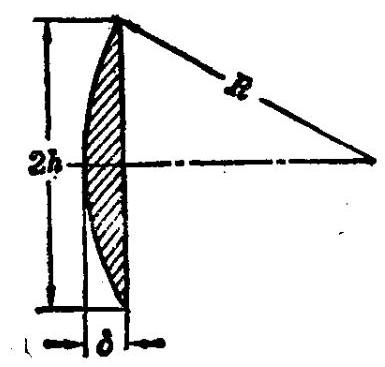
\includegraphics[max width=0.4\textwidth]{images/01912c18-5c3f-733d-b775-749ba9897a9d_128_440234.jpg}
\end{center}

(第 24 题)

24. 如图,一透镜的凸面半径是 \(R\) , 四径是 \({2h}\) ( \(h\) 比 \(R\) 小得多),厚度是 \(\delta\) . 导出近似关系式:

\[
\delta \approx \frac{{h}^{2}}{2R}
\]

\section*{\(B\) 组}

25. 证明双曲线 \({xy} = a(a\) 为不等于零的常数) 上任意一点处的切线和坐标轴所构成的三角形的面积等于 \(2\left| a\right|\) .

26. 设函数

\[
f\left( x\right) = \left\{ \begin{array}{ll} {x}^{2}, & x \leq 1; \\ {ax} + b, & x > 1. \end{array}\right.
\]

为了使 \(f\left( x\right)\) 在点 \(x = 1\) 处连续而且可导,应该怎样选取系数 \(a,b\) ?

27. 把 \(y = \arcsin x\) 变形为 \(x = \sin y\) ,利用隐函数的求导法则, 证明:

\[
{\left( \arcsin x\right) }^{\prime } = \frac{1}{\sqrt{1 - {x}^{2}}}
\]

\begin{center}
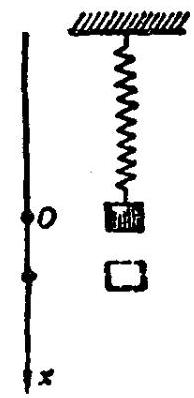
\includegraphics[max width=0.2\textwidth]{images/01912c18-5c3f-733d-b775-749ba9897a9d_129_320008.jpg}
\end{center}

(第 28 题)

28. 一质量为 3 公斤的物体挂于弹簧的下端,在 \(O\) 点上下振动,振动规律为 \(x = {10}\sin t\) . 求振动过程中的最大动能.

(位移单位为厘米, 时间单位为秒.)

29. 一倒置圆锥形的容器, 它的轴截面是一等边三角形. 以每秒 100 立方厘米的速度往容器内加水, 求当水面高度为 20 厘米时水面上升的速度. (提示: 先写出容器内水的体积与水面高度的函数关系.)

30. 从上口直径为 12 厘米, 深为 18 厘米的锥形漏斗中流出溶液, 当液面高度从 10 厘米下降到 9.8 厘米时, 求流出溶液的容积的近似值。

\chapter{导数的应用}

\section*{一阶导数的应用}

我们在初中研究了二次函数的极值问题. 在高中学过可以根据函数的图象,说出函数 \(f\left( x\right)\) 的单调区间. 现在我们学习了导数, 就可以利用导数来直接判断一般函数的单调性和极值. 为此, 先讲预备知识.

\section{预备知识}

定理 1 (罗尔 \(\Theta\) 中值定理) 如果函数 \(f\left( x\right)\) 在闭区间 \(\left\lbrack {a,b}\right\rbrack\) 上连续,在开区间 \(\left( {\mathbf{a},\mathbf{b}}\right)\) 内可导,且在两端点的函数值相等, 即 \(f\left( a\right) = f\left( b\right)\) ,那么至少存在一点 \(\xi \in \left( {a,b}\right)\) ,使 \({f}^{\prime }\left( \xi \right) = 0\) .

罗尔定理的几何意义是明显的. 若函数 \(f\left( x\right)\) 满足罗尔定理的条件,这就告诉我们,在闭区间 \(\left\lbrack {a,b}\right\rbrack\) 上有一条连续曲线 \(y = f\left( x\right)\) ,且过曲线上每一点 (端点除外)都可以作一条切线, 当曲线两端点的纵坐标相等时, 那么在曲线上至少能找到一点 \(\left( {\xi ,f\left( \xi \right) }\right) ,\xi \in \left( {a,b}\right)\) ,使曲线在该点的切线平行于 \(x\) 轴 (图 3-1(1)).

如果函数 \(y = f\left( x\right)\) 在区间 \(\left\lbrack {a,b}\right\rbrack\) 上罗尔定理的条件不全满足,那么在区间 \(\left( {a,b}\right)\) 内就可能任何点的切线都不与 \(x\) 轴平行(图 3-1(2)).

\customfootnote{

\begin{itemize}
\item 罗尔 (M. Rolle, 1652-1719 年), 法国数学家.
\end{itemize}

}

\begin{center}
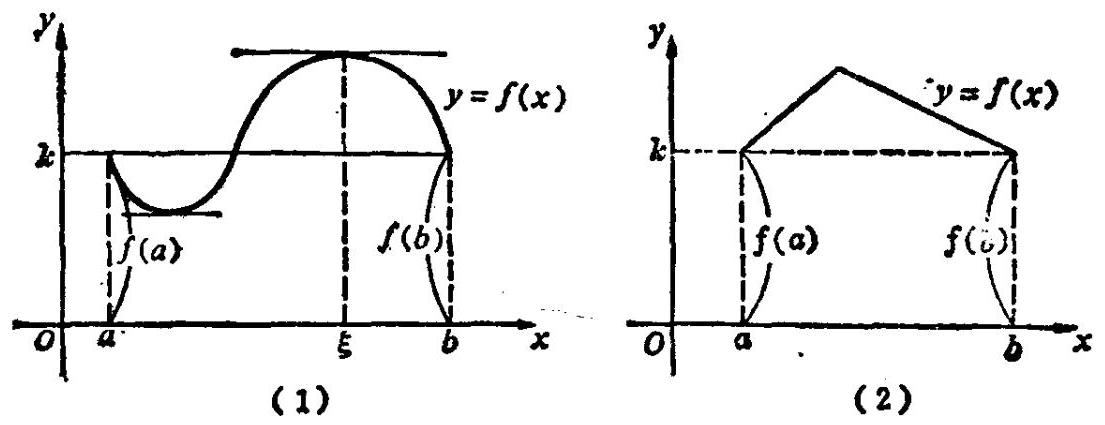
\includegraphics[max width=1.0\textwidth]{images/01912c18-5c3f-733d-b775-749ba9897a9d_131_852004.jpg}
\end{center}

图 3-1

*证明: 令 \(f\left( a\right) = f\left( b\right) = k\) ,分如下三种情况证明:

1. 在闭区间 \(\left\lbrack {a,b}\right\rbrack\) 上,恒有 \(f\left( x\right) = k\) 的情况

这时, \(f\left( x\right)\) 是 \(\left\lbrack {a,b}\right\rbrack\) 上的常数函数,于是 \({f}^{\prime }\left( x\right) = 0\) ,因此罗尔定理对开区间 \(\left( {a,b}\right)\) 内任何点皆成立.

2. 在 \(\left\lbrack {a,b}\right\rbrack\) 上有点 \(x\) ,使得 \(f\left( x\right) > k\) 的情况

因为 \(f\left( x\right)\) 为 \(\left\lbrack {a,b}\right\rbrack\) 上的连续函数,根据连续函数性质 1, 得知在 \(\left\lbrack {a,b}\right\rbrack\) 上存在点 \(\left( {{\xi }_{1},f\left( {\xi }_{1}\right) }\right)\) 为 \(f\left( x\right)\) 在 \(\left\lbrack {a,b}\right\rbrack\) 上的最大值,即 当 \(a \leq x \leq b\) 时,

\[
f\left( x\right) \leq f\left( {\xi }_{1}\right) , \tag{1}
\]

又因在 \(\left\lbrack {a,b}\right\rbrack\) 上有点 \(x\) ,使得

\[
f\left( x\right) > k, \tag{2}
\]

由 (1)、(2) 式得 \(f\left( {\xi }_{1}\right) > k\) ,这说明点 \({\xi }_{1}\) 不可能是 \(\left\lbrack {a,b}\right\rbrack\) 的端点,从而 \(a < {\xi }_{1} < b\) . 现证

\[
{f}^{\prime }\left( {\xi }_{1}\right) = 0\text{.}
\]

当 \(a \leq {\xi }_{1} + {\Delta x} \leq b\) 时,对于 \({\Delta x} > 0\) (或 \({\Delta x} < 0\) ) 由 (1) 式总有

\[
{\Delta y} = f\left( {{\xi }_{1} + {\Delta x}}\right) - f\left( {\xi }_{1}\right) \leq 0,
\]

设 \({\Delta x} > 0\) ,则 \(\frac{\Delta y}{\Delta x} \leq 0\) ,于是 \(\mathop{\lim }\limits_{{{\Delta x} \rightarrow 0 + }}\frac{\Delta y}{\Delta x} \leq 0\) .

若 \({\Delta x} < 0\) ,则 \(\frac{\Delta y}{\Delta x} \geq 0\) ,于是 \(\mathop{\lim }\limits_{{{\Delta x} \rightarrow 0}}\frac{\Delta y}{\Delta x} \geq 0\) .

又因 \(a < {\xi }_{1} < b\) ,根据定理的条件可知 \({f}^{\prime }\left( {\xi }_{1}\right)\) 存在,所以 \({f}^{\prime }\left( {\xi }_{1}\right) = 0\) . 取 \(\xi = {\xi }_{1}\) ,定理得证.

3. 在 \(\left\lbrack {a,b}\right\rbrack\) 上有点 \(x\) ,使得 \(f\left( x\right) < k\) 的情况

由连续函数性质 1,得知在 \(\left\lbrack {a,b}\right\rbrack\) 上存在点 \({\xi }_{2},f\left( {\xi }_{2}\right)\) 为 \(f\left( x\right)\) 在 \(\left\lbrack {a,b}\right\rbrack\) 上的最小值. 与情况 2 类似,容易证明

\[
{f}^{\prime }\left( {\xi }_{2}\right) = 0
\]

再取 \(\xi = {\xi }_{2}\) ,定理证完.

这个定理告诉我们, 如果定理所要求的条件满足, 那么方程

\[
{f}^{\prime }\left( x\right) = 0,
\]

在 \(\left( {a,b}\right)\) 内至少有一个实数根. 我们把方程 \({f}^{\prime }\left( x\right) = 0\) 的根称为函数 \(f\left( x\right)\) 的驻点(图 3-1(1)).

例 1 验证函数 \(f\left( x\right) = {x}^{2} - {4x}\) 在区间 \(\left\lbrack {1,3}\right\rbrack\) 上是否满足罗尔定理的条件,如果满足,求区间 \(\left( {1,3}\right)\) 内满足罗尔定理的 \(\xi\) 值.

解: 函数 \(f\left( x\right) = {x}^{2} - {4x}\) 在闭区间 \(\left\lbrack {1,3}\right\rbrack\) 上连续,在 \(\left( {1,3}\right)\) 内可导,故满足罗尔定理的所有条件,且 \({f}^{\prime }\left( x\right) = {2x} - 4\) ,所以, 根据定理至少存在一点 \(\xi ,\xi \in \left( {1,3}\right)\) ,为方程 \({f}^{\prime }\left( x\right) = {2x} - 4 = 0\) 的根. 因此 \(x = 2\) 就是所求的 \(\xi\) 。

定理 2 (拉格朗日 \(\mathbf{O}\) 中值定理) 如果函数 \(f\left( x\right)\) 在闭区间 \(\left\lbrack {a,b}\right\rbrack\) 上连续,在开区间 \(\left( {a,b}\right)\) 内可导,那么在 \(\left( {a,b}\right)\) 内至少有一点 \(\xi\) ,使得

\[
{f}^{\prime }\left( \xi \right) = \frac{f\left( b\right) - f\left( a\right) }{b - a}.
\]

这个定理的几何意义也是明显的. 因为已知导数 \({f}^{\prime }\left( \xi \right)\) 的几何意义是曲线 \(y = f\left( x\right)\) 在点 \(\left( {\xi ,f\left( \xi \right) }\right)\) 处切线的斜率,而 \(\frac{f\left( b\right) - f\left( a\right) }{b - a}\) 表示 \({AB}\) 弦的斜率. 这样如果函数 \(f\left( x\right)\) 满足拉格朗日定理的条件,这就告诉我们,在闭区间 \(\left\lbrack {a,b}\right\rbrack\) 上有一连续曲线,且过曲线 \(y = f\left( x\right)\) 上每一点(端点除外)都可以作一条切线, 那么在曲线上至少有一点 \(M\left( {\xi ,f\left( \xi \right) }\right) ,\xi \in \left( {a,b}\right)\) ,使得过点 \(M\) 的切线与弦 \({AB}\) 平行 (图 \(3 - 2)\) .

\begin{center}
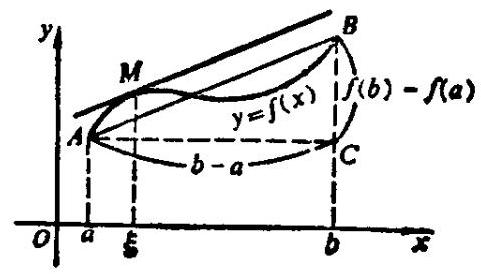
\includegraphics[max width=0.5\textwidth]{images/01912c18-5c3f-733d-b775-749ba9897a9d_133_982068.jpg}
\end{center}

图 3-2

分析: 从罗尔定理和拉格朗日定理的条件与几何解释可以看出, 罗尔定理是拉格朗日定理的特殊情形. 因为如果函数 \(f\left( x\right)\) 在区间 \(\left\lbrack {a,b}\right\rbrack\) 上满足拉格朗日定理条件,且 \(f\left( x\right)\) 在两端点的函数值相等,即 \(f\left( a\right) = f\left( b\right)\) 时,函数 \(f\left( x\right)\) 在区间 \(\left\lbrack {a,b}\right\rbrack\) 上也满足罗尔定理条件, 所以这种情形的拉格朗日定理就是罗尔定理. 下边就利用罗尔定理来证明拉格朗日定理. 为此, 我们作个辅助函数:

\[
\varphi \left( x\right) = f\left( x\right) - {kx},
\]

并适当选择待定系数 \(k\) ,使函数 \(\varphi \left( x\right)\) 满足罗尔定理的所有条件.

\customfootnote{

拉格朗日 (J. L. Lagrange, 1736-1813 年), 法国数学家.

}

因 \(f\left( x\right) \text{、}{kx}\) 在 \(\left\lbrack {a,b}\right\rbrack\) 上连续,在 \(\left( {a,b}\right)\) 内可导,所以函数 \(\varphi \left( x\right) = f\left( x\right) - {kx}\) 在 \(\left\lbrack {a,b}\right\rbrack\) 上连续,在 \(\left( {a,b}\right)\) 内可导,为了使 \(\varphi \left( a\right) = \varphi \left( b\right)\) 也成立,则必须且只须使

\[
f\left( a\right) - {ka} = f\left( b\right) - {kb},
\]

即

\[
k = \frac{f\left( b\right) - f\left( a\right) }{b - a}.
\]

证明: 作辅助函数:

\[
\varphi \left( x\right) = f\left( x\right) - \frac{f\left( b\right) - f\left( a\right) }{b - a}x,
\]

由前面分析可知, \(\varphi \left( x\right)\) 在 \(\left\lbrack {a,b}\right\rbrack\) 上连续,在 \(\left( {a,b}\right)\) 内可导,且 \(\varphi \left( a\right) = \varphi \left( b\right)\) ,即罗尔定理的条件皆满足,根据罗尔定理可知, 至少存在一点 \(\xi \in \left( {a,b}\right)\) ,使 \({\varphi }^{\prime }\left( \xi \right) = 0\) ,

但

\[
{\varphi }^{\prime }\left( x\right) = {f}^{\prime }\left( x\right) - \frac{f\left( b\right) - f\left( a\right) }{b - a},
\]

于是

\[
{\varphi }^{\prime }\left( \xi \right) = {f}^{\prime }\left( \xi \right) - \frac{f\left( b\right) - f\left( a\right) }{b - a} = 0,
\]

所以证得

\[
{f}^{\prime }\left( \xi \right) = \frac{f\left( b\right) - f\left( a\right) }{b - a}.
\]

\begin{itemize}
\item 这个定理告诉我们, 如果定理所要求的条件已满足, 那么,在 \(\left( {a,b}\right)\) 内至少存在一个点 \(\xi\) ,当 \(x = \xi\) 时,等式
\end{itemize}

\[
{f}^{\prime }\left( \xi \right) = \frac{f\left( b\right) - f\left( a\right) }{b - a}
\]

成立, 也就是说方程

\[
{f}^{\prime }\left( x\right) = \frac{f\left( b\right) - f\left( a\right) }{b - a}
\]

在 \(\left( {a,b}\right)\) 内至少有一个实根.

为了便于应用, 拉格朗日定理的结论, 通常写成如下形式:

\[
f\left( b\right) - f\left( a\right) = {f}^{\prime }\left( \xi \right) \left( {b - a}\right) ,\;a < \xi < b.
\]

例 2 求函数 \(f\left( x\right) = {x}^{3}\) 在 \(\left( {-1,2}\right)\) 内,满足中值定理 \(f\left( b\right) - f\left( a\right) = {f}^{\prime }\left( \xi \right) \left( {b - a}\right)\) 的点 \(\xi\) 的值.

解: 因为 \({f}^{\prime }\left( x\right) = 3{x}^{2},f\left( 2\right) = 8,f\left( {-1}\right) = - 1\) , 满足中值定理的 \(\xi\) 应有,

\[
f\left( 2\right) - f\left( {-1}\right) = 3{\xi }^{2}\left\lbrack {2 - \left( {-1}\right) }\right\rbrack ,
\]

即

\[
9 = 9{\xi }^{2}
\]

得

\[
\xi = \pm 1\text{.}
\]

\[
1 \in \left( {-1,2}\right) , - 1 \notin \left( {-1,2}\right) ,
\]

\begin{center}
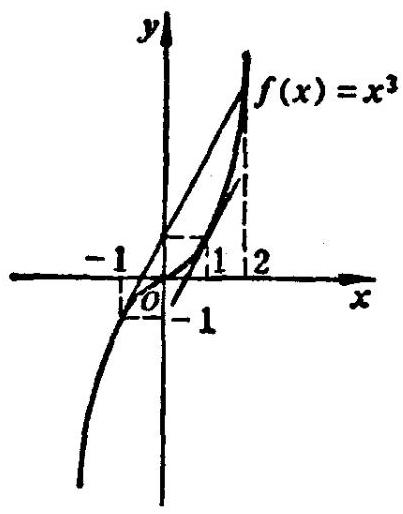
\includegraphics[max width=0.4\textwidth]{images/01912c18-5c3f-733d-b775-749ba9897a9d_135_695444.jpg}
\end{center}

图 3-3

所以 \(\xi = 1\) .

*例3 当 \(x > 1\) 时,证明不等式 \({e}^{x} > {ex}\) 成立.

解: 令 \(f\left( x\right) = {e}^{x}\) ,

则 \({f}^{\prime }\left( x\right) = {e}^{x}\) ,

由于函数 \(f\left( x\right) = {e}^{x}\) 在区间 \(\left\lbrack {1,x}\right\rbrack\)

上满足拉格朗日定理条件, 所以

在 \(\left( {1,x}\right)\) 内至少存在一点 \(\xi\) ,使

\[
{e}^{x} - {e}^{1} = {e}^{\xi }\left( {x - 1}\right) \tag{1}
\]

成立,又 \({e}^{x}\) 为增函数,且 \(1 < \xi < x\) ,于是

\[
{e}^{1} < {e}^{\xi } \tag{2}
\]

将 (2) 式代入 (1) 式得 \({e}^{x} - e > e\left( {x - 1}\right)\) .

即

\[
{e}^{x} > {ex}\text{.}
\]

\begin{problemset}[练习]

\item 说明下列函数在给定区间上, 罗尔定理是否成立. 如果成立,求 \(\xi\) 值; 如果不成立,说明理由:

(1) \(f\left( x\right) = \sin x,x \in \left\lbrack {0,{2\pi }}\right\rbrack\) ;

(2) \(f\left( x\right) = \left| x\right| ,x \in \left\lbrack {-1,1}\right\rbrack\) ;

(3) \(f\left( x\right) = {x}^{3},x \in \left\lbrack {0,1}\right\rbrack\) ; (4) \(f\left( x\right) = \left\{ \begin{array}{ll} {x}^{2}, & x \in (0,1\rbrack , \\ 1, & x = 0. \end{array}\right.\)

\item 如果函数 \(f\left( x\right)\) 满足下列条件之一,讨论拉格朗日中值定理是否成立:

(1)函数 \(f\left( x\right)\) 在 \(\left( {a,b}\right)\) 内可导;

(2)函数 \(f\left( x\right)\) 在 \(\left\lbrack {a,b}\right\rbrack\) 上可导;

(3)函数 \(f\left( x\right)\) 在 \((a,b\rbrack\) 可导;

(4)函数 \(f\left( x\right)\) 在 \(\lbrack a,b)\) 可导.

\item 求函数 \(f\left( x\right) = {x}^{3} + {2x}\) 在下列区间内,满足拉格朗日中值定理的 \(\xi\) 值.

(1) \(\left\lbrack {0,1}\right\rbrack\) ; (2) \(\left\lbrack {1,2}\right\rbrack\) ; (3) \(\left\lbrack {-1,2}\right\rbrack\) .

\end{problemset}

\begin{problemset}[习 题 九]

\item 对下列函数检验罗尔定理是否成立:

(1) \(f\left( x\right) = \left( {x - 1}\right) \left( {x - 2}\right) ,\;x \in \left\lbrack {1,2}\right\rbrack\) ;

(2) \(f\left( x\right) = \left| x\right| - 1\) , \(\;x \in \left\lbrack {-1,1}\right\rbrack\) ;

(3) \(f\left( x\right) = \sqrt[3]{{x}^{2}},\;x \in \left\lbrack {-1,1}\right\rbrack\) ;

(4) \(f\left( x\right) = x - \left\lbrack x\right\rbrack ,\;x \in \left\lbrack {0,1}\right\rbrack\) .

\item 求出函数 \(f\left( x\right) = {x}^{3}\) 在区间 \(\left\lbrack {a,b}\right\rbrack\) 内,满足拉格朗日中值定理的 \(\xi\) 值。

\item 求下列函数满足 \(f\left( b\right) - f\left( a\right) = {f}^{\prime }\left( \xi \right) \left( {b - a}\right) ,a < \xi < b\) 的 \(\xi\) 值:

(1) \(f\left( x\right) = {x}^{2} - {2x} + 2,\;a = - 1,\;b = 1\) ;

(2) \(f\left( x\right) = {x}^{3} - {x}^{2},\;a = 0,\;b = 1\) ;

(3) \(f\left( x\right) = \frac{6}{x},\;a = 2,\;b = 3\) .

\item 利用拉格朗日中值定理, 证明下列不等式:

(1) \(\left| {\sin {x}_{1} - \sin {x}_{2}}\right| \leq \left| {{x}_{1} - {x}_{2}}\right|\) ;

(2) \(\left| {\operatorname{arctg}{x}_{1} - \operatorname{arctg}{x}_{2}}\right| \leq \left| {{x}_{1} - {x}_{2}}\right|\) ;

(3)当 \(0 \leq a < b\) 时,

\[
{e}^{b} - {e}^{a} > b - a.
\]

\item 证明: 若函数 \(f\left( x\right)\) 在 \(\left\lbrack {a,b}\right\rbrack\) 上有二阶导数,且 \(f\left( a\right) =\) \(f\left( b\right) = 0,f\left( c\right) = 0\left( {a < c < b}\right)\) ,则在 \(\left( {a,b}\right)\) 内至少存在一点 \(\xi\) , 使得 \({f}^{\prime \prime }\left( \xi \right) = 0\) .

\end{problemset}

\section{函数的单调性}

我们已经学过增函数与减函数的概念, 现在学习利用导数来判断函数的增减性(即函数的单调性). 有如下一个重要的定理.

定理 设函数 \(f\left( x\right)\) 在区间 \(\left( {\mathbf{a},\mathbf{b}}\right)\) 内可导. 如果在 \(\left( {\mathbf{a},\mathbf{b}}\right)\) 内 \({f}^{\prime }\left( x\right) > 0\) ,那么 \(f\left( x\right)\) 在 \(\left( {a,b}\right)\) 内是增函数; 如果在 \(\left( {a,b}\right)\) 内 \({f}^{\prime }\left( x\right) < 0\) ,那么 \(f\left( x\right)\) 在 \(\left( {a,b}\right)\) 内是减函数.

如果在 \(\left( {\mathbf{a},\mathbf{b}}\right)\) 内恒有 \({\mathbf{f}}^{\prime }\left( \mathbf{x}\right) = \mathbf{0}\) ,那么 \(\mathbf{f}\left( \mathbf{x}\right)\) 在 \(\left( {\mathbf{a},\mathbf{b}}\right)\) 内是常数.

证明: 在区间 \(\left( {a,b}\right)\) 内任取两点 \({x}_{1},{x}_{2}\) ,且使 \({x}_{1} < {x}_{2}\) ,根据拉格朗日中值定理, 可得

\[
f\left( {x}_{2}\right) - f\left( {x}_{1}\right) = {f}^{\prime }\left( \xi \right) \left( {{x}_{2} - {x}_{1}}\right) ,\;\left( {{x}_{1} < \xi < {x}_{2}}\right) . \tag{1}
\]

如果在区间 \(\left( {a,b}\right)\) 内 \({f}^{\prime }\left( x\right) > 0\) ,则 \(\left( 1\right)\) 式中的 \({f}^{\prime }\left( \xi \right) > 0\) ,而 \({x}_{2} - {x}_{1} > 0\) ,因此由 (1) 式可知 \(f\left( {x}_{2}\right) > f\left( {x}_{1}\right)\) . 这就是说, \(f\left( x\right)\) 在区间 \(\left( {a,b}\right)\) 内是增函数.

如果在区间 \(\left( {a,b}\right)\) 内 \({f}^{\prime }\left( x\right) < 0\) ,则 \(\left( 1\right)\) 式中的 \({f}^{\prime }\left( \xi \right) < 0\) ,而 \({x}_{2} - {x}_{1} > 0\) ,因此由 (1) 式可知 \(f\left( {x}_{2}\right) < f\left( {x}_{1}\right)\) . 这就是说, \(f\left( x\right)\) 在区间 \(\left( {a,b}\right)\) 内是减函数.

如果在区间 \(\left( {a,b}\right)\) 内恒有 \({f}^{\prime }\left( x\right) = 0\) ,则 \(\left( 1\right)\) 式中的 \({f}^{\prime }\left( \xi \right) =\) 0,因此由 (1) 式可知 \(f\left( {x}_{2}\right) = f\left( {x}_{1}\right)\) . 这就是说,在区间 \(\left( {a,b}\right)\) 内,任意两点的函数值相等. 因此, \(f\left( x\right)\) 在区间 \(\left( {a,b}\right)\) 内是常数.

例 1 确定函数 \(y = {x}^{2} - {2x} + 4\) 在哪个区间内 是增函数, 哪个区间内是减函数.

\begin{center}
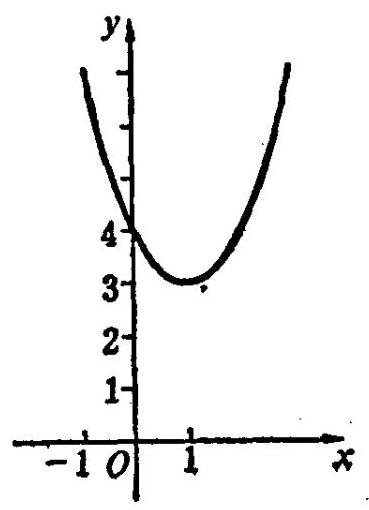
\includegraphics[max width=0.4\textwidth]{images/01912c18-5c3f-733d-b775-749ba9897a9d_138_431329.jpg}
\end{center}

图 3-4

解: 将 \(y\) 对 \(x\) 求导,得

\[
{y}^{\prime } = {2x} - 2
\]

解不等式 \({y}^{\prime } = {2x} - 2 > 0\) , 得 \(x > 1\) ,因此 \(y\) 在 \(\left( {1, + \infty }\right)\) 内是增函数;

解不等式 \({y}^{\prime } = {2x} - 2 < 0\) , 得 \(x < 1\) ,因此 \(y\) 在 \(\left( {-\infty ,1}\right)\) 内是减函数 (图 3-4).

例 2 确定函数 \(y = \frac{2}{a}\left( {x \neq 0}\right)\) 的增减范围,

解: \({y}^{\prime } = - \frac{2}{{x}^{2}}\) .

\begin{center}
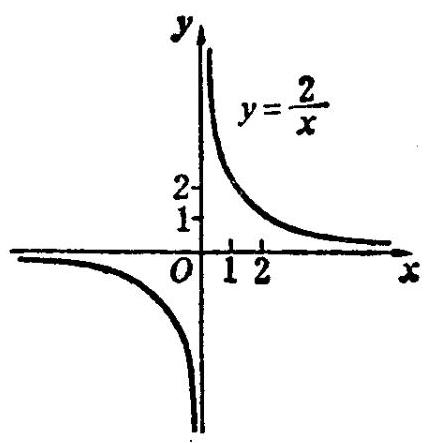
\includegraphics[max width=0.4\textwidth]{images/01912c18-5c3f-733d-b775-749ba9897a9d_139_324623.jpg}
\end{center}

图 3-5

由于 \(x \neq 0\) 时,有 \(- \frac{2}{{x}^{2}} < 0\) ,

\(y\) 在 \(\left( {-\infty ,0}\right) ,\left( {0, + \infty }\right)\) 内都是减函数 (图 3-5).

*例 3 当 \(x > 0\) 时,证明不等式

\[
\ln \left( {1 + x}\right) > x - \frac{1}{2}{x}^{2}
\]

成立.

证明: 设 \(f\left( x\right) = \ln \left( {1 + x}\right) - x + \frac{1}{2}{x}^{2}\) ,

则

\[
{f}^{\prime }\left( x\right) = \frac{1}{1 + x} - 1 + x = \frac{{x}^{2}}{1 + x}.
\]

当 \(x > 0\) 时, \({f}^{\prime }\left( x\right) > 0\) ,因此 \(f\left( x\right)\) 在 \(\left( {0, + \infty }\right)\) 内为增函数. 又 \(f\left( x\right)\) 在点 \(x = 0\) 处连续,所以 \(f\left( x\right)\) 在 \(\lbrack 0, + \infty )\) 上也是增函数. 于是当 \(x > 0\) 时, \(f\left( x\right) > f\left( 0\right)\) ,

\[
\because f\left( 0\right) = 0,\;\therefore f\left( x\right) > 0,
\]

即

\[
\ln \left( {1 + x}\right) - x + \frac{1}{2}{x}^{2} > 0,
\]

于是证得

\[
\ln \left( {1 + x}\right) > x - \frac{1}{2}{x}^{2}
\]

\begin{problemset}[练习]

\item 根据三角函数在各象限内的值的符号, 利用导数证明函数 \(y = \cos x\) 在开区间 \(\left( {\frac{\pi }{2},\pi }\right)\) 内是减函数.

\item 确定下列函数的增减范围 (不必画出图象):

(1) \(y = \frac{1}{2{x}^{2}}\left( {x \neq 0}\right)\) ; (2) \(y = x - {x}^{3}\) ;

(3) \(y = \ln \left( {{2x} - 1}\right)\) ; (4) \(y = - {e}^{x}\) .

\item 已知函数 \(y = a{x}^{2}\left( {a \neq 0}\right)\) 当 \(x > 0\) 时是减函数,利用求导数的方法确定 \(a\) 的值的范围.

\item 求下列函数的驻点:

(1) \(y = 5{x}^{2} - {4x} + 1\) ; (2) \(y = {x}^{3} - {27x}\) .

\item* 当 \(x > 0\) 时,证明下列不等式成立:

(1) \(\sin x > x - \frac{{x}^{3}}{6}\) ;

(2) \(\cos x < 1 - \frac{{x}^{2}}{2} + \frac{{x}^{4}}{24}\)

(3) \({\mathrm{e}}^{x} > 1 + x + \frac{{x}^{2}}{2}\) .


\end{problemset}

\section{函数的极大值与极小值}

如果函数 \(y = f\left( x\right)\) 在点 \({x}_{0}\) 处连续,并且 \({x}_{0}\) 不是其定义区间的端点. 若对 \({x}_{0}\) 附近的所有点 \(x\left( {x \neq {x}_{0}}\right)\) ,都有

\[
f\left( x\right) < f\left( {x}_{0}\right) \;\text{ (或 }f\left( x\right) > f\left( {x}_{0}\right) \text{ ),}
\]

我们就说函数 \(f\left( x\right)\) 在点 \({x}_{0}\) 处取极大值 (或极小值). 也可以说 \(f\left( {x}_{0}\right)\) 是函数 \(f\left( x\right)\) 的一个极大值 (或极小值),记作 \({y}_{\text{极大 }} =\) \(f\left( {x}_{0}\right)\) (或 \({y}_{\text{极小 }1} = f\left( {x}_{0}\right)\) ),并把点 \({x}_{0}\) 称为函数 \(f\left( x\right)\) 的一个极大点(或极小点). 极大值与极小值统称为极值. 极大点与极小点统称为极值点. 图 3-6 和图 3-7 分别显示了可导函数在点 \({x}_{0}\) 处取极大值与极小值的情况.

从图 3-6-和图 3-7 可以看出,可导函数 \(f\left( x\right)\) 的曲线在它

\begin{center}
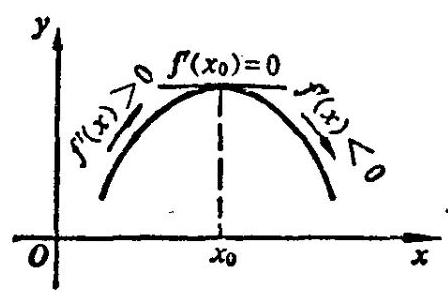
\includegraphics[max width=0.4\textwidth]{images/01912c18-5c3f-733d-b775-749ba9897a9d_141_386711.jpg}
\end{center}

图 3-6

\begin{center}
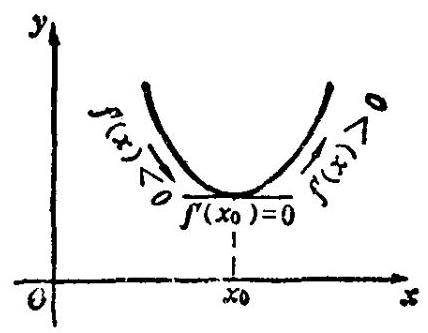
\includegraphics[max width=0.4\textwidth]{images/01912c18-5c3f-733d-b775-749ba9897a9d_141_950727.jpg}
\end{center}

图 3-7

的极值点 \({x}_{0}\) 处的切线都平行于 \(x\) 轴,即 \({f}^{\prime }\left( {x}_{0}\right) = 0\) . 换句话说, 可导函数的极值点一定是它的驻点. 但是, 反过来, 可导函数的驻点, 却不一定是它的极值点. 如 \(f\left( x\right) = {x}^{3}\) 的导数是 \({f}^{\prime }\left( x\right) = 3{x}^{2}\) ,在 \(x = 0\) 处有 \({f}^{\prime }\left( 0\right) = 0\) ,即点 \(x = 0\) 是函数 \(f\left( x\right) = {x}^{3}\) 的驻点, 但并不是它的极值点 (图 3- 8).

\begin{center}
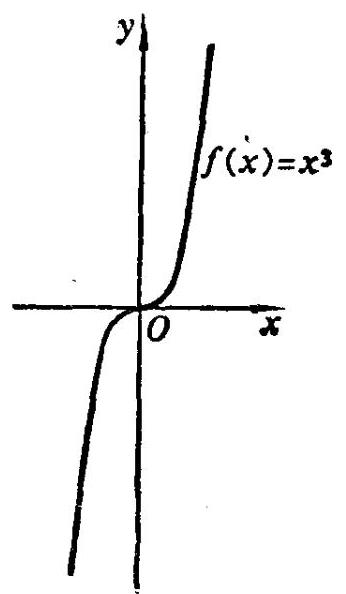
\includegraphics[max width=0.3\textwidth]{images/01912c18-5c3f-733d-b775-749ba9897a9d_141_203287.jpg}
\end{center}

图 3-8

因此, 在求可导函数的极值时, 除了 \({f}^{\prime }\left( x\right) = 0\) 的条件外,还要考虑 \({f}^{\prime }\left( x\right)\) 在驻点 \({x}_{0}\) 两侧的正负情况: 如果 \({f}^{\prime }\left( {x}_{0}\right) = 0\) ,并且 \(x\) 由小变大经过 \({x}_{0}\) 时, \({f}^{\prime }\left( x\right)\) 由正变为负 (或由负变为正),那么 \(f\left( x\right)\) 在点 \({x}_{0}\) 必然取得极大值 (或极小值).

综上所述, 并根据上节定理 (参看图 3-6 和图 3-7), 我们得到求可导函数 \(f\left( x\right)\) 的极值的方法如下:

1. 求导数 \({f}^{\prime }\left( x\right)\) ;

2. 求 \(f\left( x\right)\) 在定义域内的驻点;

3. 检查 \({f}^{\prime }\left( x\right)\) 在驻点左右的符号,如果左正右负,那么 \(f\left( x\right)\) 在这个驻点取极大值;

如果左负右正,那么 \(f\left( x\right)\) 在这个驻点取极小值;

如果左右同号,那么 \(f\left( x\right)\) 在这个驻点的函数值不是极值.

例 1 求函数 \(f\left( x\right) = \frac{1}{3}{x}^{3} - {4x} + 4\) 的极值.

解: \(f\left( x\right)\) 是可导函数,令

\[
{f}^{\prime }\left( x\right) = {x}^{2} - 4 = \left( {x + 2}\right) \left( {x - 2}\right) = 0,
\]

解得驻点为 \({x}_{1} = - 2,{x}_{2} = 2\) .

当 \(x\) 变化时, \({f}^{\prime }\left( x\right) ,f\left( x\right)\) 的变化状态如下表:

\begin{center}
\adjustbox{max width=\textwidth}{
\begin{tabular}{|c|c|c|c|c|c|}
\hline
\(x\) & \(\left( {-\infty , - 2}\right)\) & \(- 2\) & \(\left( {-2,2}\right)\) & 2 & \(\left( {2, + \infty }\right)\) \\
\hline
\({f}^{\prime }\left( x\right)\) & \(+\) & 0 & \(-\) & 0 & \(+\) \\
\hline
\(f\left( x\right)\) & 1 & 极大值 \(9\frac{1}{3}\) & / & 极小值 \(- 1\frac{1}{3}\) & 1 \\
\hline
\end{tabular}
}
\end{center}

因此当 \(x = - 2\) 时,函数 \(f\left( x\right)\) 有极大值,且

\[
f\left( {-2}\right) = \frac{1}{3}{\left( -2\right) }^{3} - 4\left( {-2}\right) + 4 = 9\frac{1}{3}
\]

而当 \(x = 2\) 时,函数 \(f\left( x\right)\) 有极小值, 且 \(f\left( 2\right) = \frac{1}{3} \cdot {2}^{3} - 4 \cdot 2 + 4 = - 1\frac{1}{3}\) .

\begin{center}
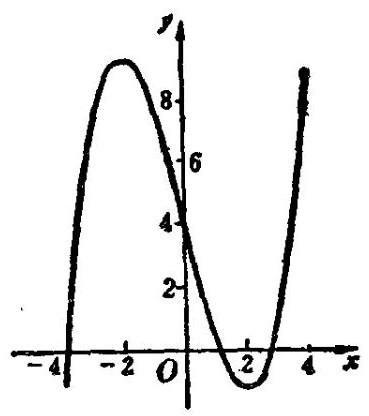
\includegraphics[max width=0.4\textwidth]{images/01912c18-5c3f-733d-b775-749ba9897a9d_143_629914.jpg}
\end{center}

图 3-9

函数 \(f\left( x\right) = \frac{1}{3}{x}^{3} - {4x} + 4\) 的图象如图 3-9 所示.

例 2 求函数 \(f\left( x\right) = x + 2\sin x\) 在区间 \(\left\lbrack {0,{2\pi }}\right\rbrack\) 内的极值.

解: 因 \({f}^{\prime }\left( x\right) = 1 + 2\cos x\) ,

令 \(1 + 2\cos x = 0\) ,解得驻点为

\({x}_{1} = \frac{2}{3}\pi ,\;{x}_{2} = \frac{4}{3}\pi .\)

当 \(x\) 变化时, \({f}^{\prime }\left( x\right) ,f\left( x\right)\) 的变化状态如下表:

\begin{center}
\adjustbox{max width=\textwidth}{
\begin{tabular}{|c|c|c|c|c|c|c|c|}
\hline
\(x\) & 0 & . & \(\frac{2}{3}\pi\) & : & \(\frac{4}{3}\pi\) & : & \({2\pi }\) \\
\hline
\({f}^{\prime }\left( x\right)\) & \phantom{X} & \(+\) & 0 & - & 0 & \(+\) & \phantom{X} \\
\hline
\(f\left( x\right)\) & 0 & 7 & 极大值 \(\frac{2}{3}\pi + \sqrt{3}\) & y & 极小值 \(\frac{4}{3}\pi - \sqrt{3}\) & 7 & \({2\pi }\) \\
\hline
\end{tabular}
}
\end{center}

因此 当 \(\dot{x} = \frac{2}{3}\pi\) 时,函数 \(f\left( x\right)\) 有极大值,且

\[
f\left( {\frac{2}{3}\pi }\right) = \frac{2}{3}\pi + \sqrt{3}
\]

而当 \(x = \frac{4}{3}\pi\) 时,函数 \(f\left( x\right)\) 有极小值,且

\[
f\left( {\frac{4}{3}\pi }\right) = \frac{4}{3}\pi - \sqrt{3}.
\]

函数 \(f\left( x\right) = x + 2\sin x\) 的图象如图 3-10 所示.

\begin{center}
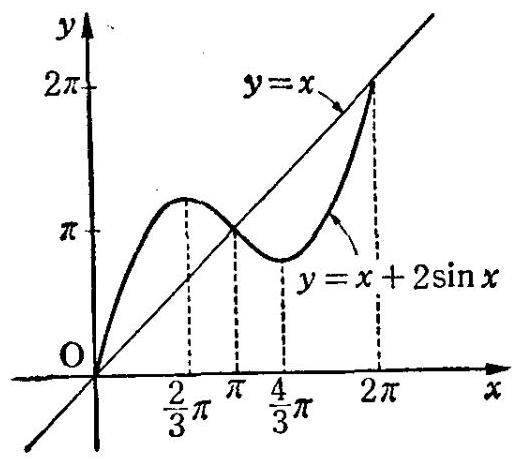
\includegraphics[max width=0.5\textwidth]{images/01912c18-5c3f-733d-b775-749ba9897a9d_144_191268.jpg}
\end{center}

图 3-10

\begin{problemset}[练习]

\item 填写下表:

\begin{center}
\adjustbox{max width=\textwidth}{
\begin{tabular}{|c|c|c|}
\hline
导 数 \({y}^{\prime }\) & 函数 \(y\) & 极 值 \\
\hline
由\_\_\_变为\_\_\_ & 由增变为减 & 极\_\_\_值 \\
\hline
由\_\_\_变为\_\_\_ & 由减变为增 & 极\_\_\_值 \\
\hline
\end{tabular}
}
\end{center}

(正, 负) (增, 减) \(\left( {大,小}\right)\)

\item 说明函数 \(y = \ln x,y = {ax} + b\) 为什么没有极值.

\item 求下列函数的极值, 并根据极值情况画出草图:

(1) \(y = {x}^{2} - {7x} + 6\) ; (2) \(y = 3{x}^{4} - 4{x}^{3}\) ;

(3) \(y = \frac{1}{2}x + \cos x\;\left( {-{2\pi } < x < {2\pi }}\right)\) .

\item 用求导数的方法证明二次函数 \(y = a{x}^{2} + {bx} + c\left( {a \neq 0}\right)\) 的

极值点为 \({x}_{0} = - \frac{b}{2a}\) ,并讨论它的极值.

\end{problemset}

\begin{problemset}[习 题 十]

\item 确定下列函数的增减范围:

(1) \(y = - {4x} + 2\) ; (2) \(y = {\left( x - 1\right) }^{2}\) ;

(3) \(y = {x}^{2} - {2x} + 5\) ; (4) \(y = {3x} - {x}^{3}\) ;

(5) \(y = {x}^{2}\left( {x - 3}\right)\) ; (6) \(y = {x}^{3} - {x}^{2} - x\) .

\item 证明下列函数的单调性:

(1) \(p\) 为何值时,函数 \(f\left( x\right) = \cos x - {px} + q\) 在整个数轴上是减函数?

(2)证明 \(y = {2x} + \sin x\) 在整个数轴上是增函数;

(3)证明 \(y = x + \frac{1}{{x}^{2} + 1}\) 在整个数轴上是增函数;

(4)研究函数 \(y = \frac{1}{{x}^{2} + x + 1}\) 的单调性.

\item 证明 \(y = \sqrt{{2x} - {x}^{2}}\) 在区间 \(\left( {0,1}\right)\) 内为增函数,在区间 \(\left( {1,2}\right)\) 内为减函数.

\item 求下列二次函数的极值:

(1) \(y = {x}^{2} - {3x} + {10}\) ; (2) \(y = - 2{x}^{2} + {4x} - 7\) ;

(3) \(y = 6{x}^{2} - x - 2\) ; (4) \(y = - {x}^{2} - {2x} + 3\) ;

(5) \(y = 2 - x - {x}^{2}\) ; (6) \(y = \frac{1}{2}{x}^{2} - {3x}\) .

\item 求下列函数的极值:

(1) \(y = 6 + {12x} - {x}^{3}\) (2) \(y = 2{x}^{2} - {x}^{4}\)

(3) \(y = 2{x}^{3} - 9{x}^{2} - {24x} - {12}\) ;

(4) \(y = \frac{1}{3}{x}^{3} - \frac{1}{2}{x}^{2} - {2x} + 2\) ;

(5) \(y = {15} + {9x} - 3{x}^{2} - {x}^{3}\) ;

(6) \(y = 4{x}^{3} - 3{x}^{2} - {6x} + 2\) ;

(7) \(y = {2x} - \sin x\) ; (8) \(y = 2{e}^{x} + {e}^{-x}\) .

\end{problemset}

\section{函数的最大值与最小值}

在生产中, 常常会遇到要求在一定条件下使“强度最大”, “用料最省”, “功率最大”这样一类问题, 在数学上, 这类问题往往归结为求函数的最大值或最小值.

本节讨论函数的最大值与最小值, 是导数应用的又一个方面. 在 3.3 节已知可导函数的极大值与极小值, 就是函数在点 \({x}_{0}\) 附近的最大值与最小值. 如图 3-11 所示. 但是,就区间 \(\left\lbrack {a,b}\right\rbrack\) 上的给定函数 \(f\left( x\right)\) 来说,函数的极大值不一定是最大值, 极小值也不一定是最小值.

\begin{center}
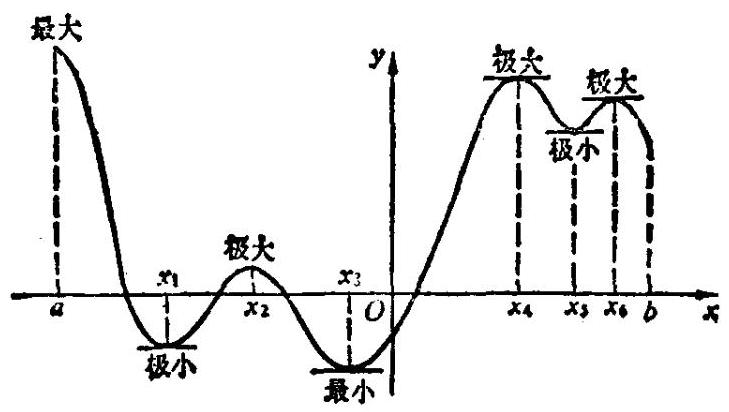
\includegraphics[max width=0.7\textwidth]{images/01912c18-5c3f-733d-b775-749ba9897a9d_146_522148.jpg}
\end{center}

图 3-11

如果函数 \(f\left( x\right)\) 在闭区间 \(\left\lbrack {a,b}\right\rbrack\) 上连续,在开区间 \(\left( {a,b}\right)\) 内可导,从连续函数性质 1 得知,函数 \(f\left( x\right)\) 在 \(\left\lbrack {a,b}\right\rbrack\) 上有最大值与最小值. 如图 3-11 中,最大值是区间端点 \(a\) 的值 \(f\left( a\right)\) ,最小值是几个极小值中最小的一个 \(f\left( {x}_{3}\right)\) . 这就是说求函数 \(f\left( x\right)\) 的最大值,只要求得所有 \(f\left( x\right)\) 的极大值与 \(f\left( a\right) \text{、}f\left( b\right)\) 这些值中最大者就行了. 而求函数 \(f\left( x\right)\) 的最小值,也只考虑 \(f\left( x\right)\) 的所有极小值与 \(f\left( a\right) \text{、}f\left( b\right)\) 中的最小者.

因此,求闭区间 \(\left\lbrack {a,b}\right\rbrack\) 上的可导函数 \(f\left( x\right)\) 在 \(\left\lbrack {a,b}\right\rbrack\) 上的最大值与最小值, 可以分两步来进行:

1. 求 \(f\left( x\right)\) 在 \(\left( {a,b}\right)\) 内的驻点;

2. 计算 \(f\left( x\right)\) 在驻点和端点的函数值,并把这些值加以比较, 其中最大的一个为最大值, 最小的一个为最小值.

因为二次函数在其定义域内只有一个极值点, 所以在包含极值点的闭区间上, 二次函数的极大值就是最大值, 极小值就是最小值, 如图 3-12 所示. 11440

\begin{center}
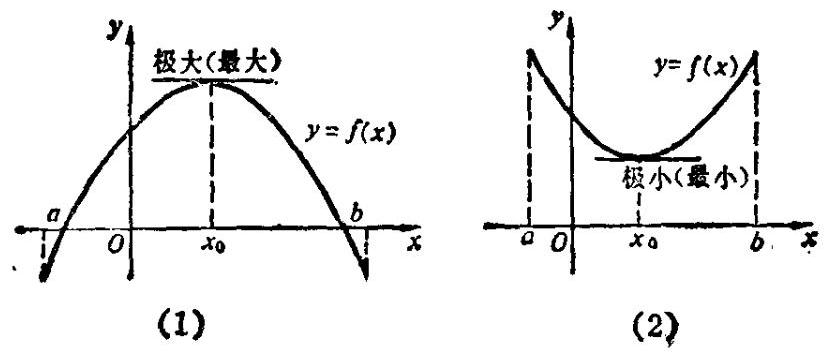
\includegraphics[max width=0.8\textwidth]{images/01912c18-5c3f-733d-b775-749ba9897a9d_147_605988.jpg}
\end{center}

图 8-12

例 1 求函数 \(y = {x}^{4} - 2{x}^{2} + 5\) 在区间 \(\left\lbrack {-2,2}\right\rbrack\) 上的最大值与最小值.

解: \({y}^{\prime } = 4{x}^{3} - {4x}\) .

令 \(4{x}^{3} - {4x} = 0\) ,求得驻点为

\[
{x}_{1} = - 1,\;{x}_{2} = 0,\;{x}_{3} = 1.
\]

这些驻点的函数值为

\[
{\left. y\right| }_{x = 0} = 5,{\left. y\right| }_{x = \pm 1} = 4\text{. }
\]

区间端点的函数值为

\[
{\left. y\right| }_{x = \pm 2} = {13}\text{.}
\]

将这些求出的函数值加以比较, 知道最大值为 13 , 最小值为 4 (图 3-13).

\begin{center}
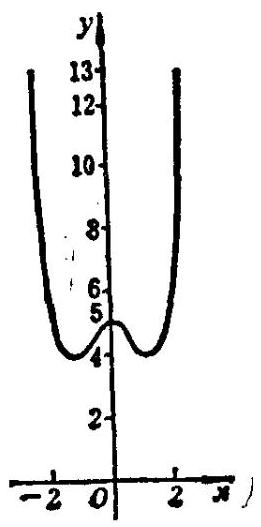
\includegraphics[max width=0.3\textwidth]{images/01912c18-5c3f-733d-b775-749ba9897a9d_148_436471.jpg}
\end{center}

图 3-13

\begin{center}
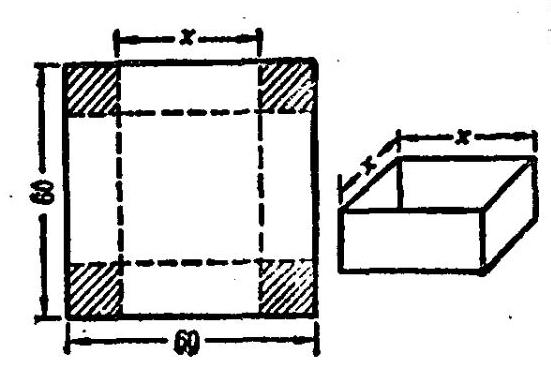
\includegraphics[max width=0.6\textwidth]{images/01912c18-5c3f-733d-b775-749ba9897a9d_148_813570.jpg}
\end{center}

图 3-14

例 2 用边长为 60 厘米的正方形铁皮做一个无盖水箱, 先在四角分别截去一个小正方形, 然后把四边翻转九十度, 再焊接而成(图 3-14). 问水箱底边的长应取多少, 才能使水箱容积最大. 最大容积是多少?

解; 设水箱底边长为 \(n\) (原米),则水箱高

\[
h = \frac{{60} - x}{2}
\]

水箱容积

\[
V = V\left( x\right) = {x}^{2}h
\]

\[
= \frac{{60}{x}^{2} - {x}^{3}}{2}\left( {0 < x < {60}}\right) \text{.}
\]

由问题的实际情况来看,如果 \(x\) 过小,水箱的底面积就很小,容积 \(V\) 也就很小; 如果 \(x\) 过大,水箱的高就很小,容积 \(V\) 也就很小. 因此,其中必有一适当的 \(x\) 值,使容积 \(V\) 取得最大值.

令

\[
{V}^{\prime }\left( x\right) = {60x} - \frac{3}{2}{x}^{2} = 0,
\]

得两个根

\[
x = 0\text{(不合题意,舍去),}x = {40}\text{,}
\]

从而在定义域 \(\left( {0,{60}}\right)\) 内,函数 \(V\left( x\right)\) 只有一个驻点

\[
x = {40}\text{(厘米).}
\]

代入函数式 \(V\left( x\right)\) ,即得.

\[
{V}_{\text{最大 }} = {\left( {40}\right) }^{2} \cdot \frac{{60} - {40}}{2} = {16000}\text{ (立方厘米). }
\]

答: 水箱底边长取 40 厘米时, 容积最大. 最大容积为 16000 立方厘米.

要注意, 如果由问题的实际情况, 可以断定可导函数在定义域开区间内存在最大 (小)值,而且 \(f\left( x\right)\) 在这个定义域开区间内又只有一个驻点, 那么立即可以断定这个驻点的函数值就是最大 (小)值. 这一点在解决某些实际问题时很有用.

例 3 矩形横梁的强度同它断面的高的平方与宽的积成正比. 要将直径为 \(d\) 的圆木锯成强度最大的横梁,断面的宽和高应是多少?

\begin{center}
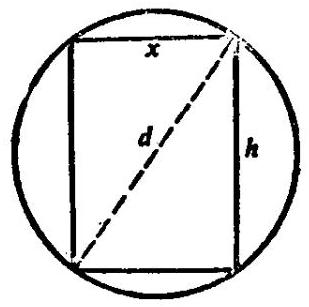
\includegraphics[max width=0.3\textwidth]{images/01912c18-5c3f-733d-b775-749ba9897a9d_150_941467.jpg}
\end{center}

图 3-15

解: 如图 3-15 所示, 设断面宽为 \(x\) ,高为 \(h\) ,则

\[
{h}^{2} = {d}^{2} - {x}^{2}
\]

横梁强度函数

\[
f\left( x\right) = {kx}{h}^{2},
\]

( \(k\) 为比例系数, \(k > 0\) ).

\(\therefore \;f\left( x\right) = {kx}\left( {{d}^{2} - {x}^{2}}\right) \;\left( {0 < x < d}\right)\) .

从实际情况可知,横梁强度函数 \(f\left( x\right)\) 在 \(\left( {0,d}\right)\) 内一定有最大值. 令

\[
{f}^{\prime }\left( x\right) = k\left( {{d}^{2} - 3{x}^{2}}\right) = 0,
\]

即 \({d}^{2} - 3{x}^{2} = 0\) ,此方程有两个根 \(x = \pm \frac{\sqrt{3}}{3}d\) ,其中负根没有意义,舍去,从而在定义域 \(\left( {0,d}\right)\) 内,函数 \(f\left( x\right)\) 只有一个驻点

\[
x = \frac{\sqrt{3}}{3}d
\]

\(f\left( x\right)\) 在这一点的函数值,就是横梁强度的最大值. 此时

\[
h = \sqrt{{d}^{2} - {x}^{2}} = \frac{\sqrt{6}}{3}d.
\]

\begin{center}
\includegraphics[max width=0.3\textwidth]{images/01912c18-5c3f-733d-b775-749ba9897a9d_150_751406.jpg}
\end{center}

图 8-16-

答: 当宽为 \(\frac{\sqrt{3}}{3}d\) ,高为 \(\frac{\sqrt{6}}{3}d\) 时,横梁强度最大.

例 4 某生产队要造一个可容纳 150 担氨水 (比重为 0.925 吨/立方米)的有盖有底圆柱形氨水槽 (图 3-16), 问氨水槽的底半径与圆柱高应取多少, 才能使所用的材料最省?

解: 材料最省, 就是使圆柱表面积最小.

设槽底半径为 \(R\) ,高为 \(h\) ,则氨水槽的表面积

\[
S = {2\pi Rh} + {2\pi }{R}^{2}.
\]

由氨水槽的容积 \(V = \pi {R}^{2}h\) ,知 \(h = \frac{V}{\pi {R}^{2}}\) ,代入上式得

\[
S = S\left( R\right) = {2\pi R}\frac{V}{\pi {R}^{2}} + {2\pi }{R}^{2}
\]

\[
= \frac{2V}{R} + {2\pi }{R}^{2}
\]

从实际情况可知,表面积 \(S\) 在其定义域内一定有最小值.

令

\[
{S}^{\prime }\left( R\right) = - \frac{2V}{{R}^{2}} + {4\pi R} = 0,
\]

即 \({2V} - {4\pi }{R}^{3} = 0\) ,此方程的实根只有一个,就是 \(R = \sqrt[3]{\frac{V}{2\pi }}\) ,因此我们得到唯一驻点

\[
R = \sqrt[3]{\frac{V}{2\pi }}
\]

当 \(R = \sqrt[3]{\frac{V}{2\pi }}\) 时,

\[
h = \frac{V}{\pi {R}^{2}} = \frac{V}{\pi {\left( \sqrt[3]{\frac{V}{2\pi }}\right) }^{2}} = \sqrt[3]{\frac{4V}{\pi }} = 2\sqrt[3]{\frac{V}{2\pi }},
\]

这就是说,当 \(h = {2R}\) 时,函数 \(S\left( R\right)\) 取得最小值,这时所用的材料最省.

现在我们根据 1 担 \(= {100}\) 斤 \(= {0.05}\) 吨,得

\[
V = {150} \times \frac{0.05}{0.925} \approx {8.11}\text{ (立方米),}
\]

于是

\[
R = \sqrt[3]{\frac{V}{2\pi }} \approx \sqrt[3]{\frac{8.11}{2\pi }} \approx {1.09}\left( \text{ 米 }\right) ,
\]

\[
h = {2R} \approx {2.18}\text{ (米) }
\]

这时建造氨水槽所用的材料最省.

答: 当氨水槽的底半径约为 1.09 米, 高约为 2.18 米时, 所用的材料最省.

例 5 已知电源电压为 \(E\) ,内电阻为 \(r\) (图 3-17),问当外电路负载电阻 \(R\) 取什么值时,输出功率最大.

\begin{center}
\includegraphics[max width=0.3\textwidth]{images/01912c18-5c3f-733d-b775-749ba9897a9d_152_349261.jpg}
\end{center}

图 3-17

解: 由欧姆定律得电流强度

\[
I = \frac{E}{R + r}.
\]

在负载电阻 \(R\) 上输出的功率

\[
P = P\left( R\right) = {I}^{2}R = \frac{{E}^{2}R}{{\left( R + r\right) }^{2}}.
\]

实验证明,当 \(E,r\) 一定时,输出功率由负载电阻 \(R\) 的大小决定. \(R\) 很小时,电源功率大都消耗在内电阻 \(r\) 上,输出功率可以变得很小; \(R\) 很大时,电路中电流很小,输出功率也可以变得很小. 因此, \(R\) 一定有一个适当的数值,使得输出功率最大. 令

\[
{P}^{\prime }\left( R\right) = {\left\lbrack \frac{{E}^{2}R}{{\left( R + r\right) }^{2}}\right\rbrack }^{\prime }
\]

\[
= {E}^{2} \cdot \frac{{\left( R + r\right) }^{2} - {2R}\left( {R + r}\right) }{{\left( R + r\right) }^{4}}
\]

\[
= {E}^{2} \cdot \frac{r - R}{{\left( R + r\right) }^{3}} = 0,
\]

即 \({E}^{2}\left( {r - R}\right) = 0\) ,求得唯一驻点

\[
R = r\text{.}
\]

所以,当 \(R = r\) ,即外电路负载电阻等于内电阻时,输出功率最大.

答: 当外电路负载电阻 \(R\) 等于内电阻 \(r\) 时,输出功率最大.

\begin{problemset}[练习]

\item 已知函数 \(y = 3{x}^{3} - {9x} + 5\) ,求函数在 \(\left\lbrack {-2,2}\right\rbrack\) 上的最大值与最小值。

\item 把长度为 \(l\) 的线段分成两段,使得以这两段分别作为长与宽所得的矩形的面积最大.

\item 把长为 \(l\) 的铁丝分成两段,各围成一个正方形,问怎样分法才能使它们的面积之和最小。

\item 等腰三角形的周长为 \({2p}\) ,问绕这个三角形的底边旋转一周所成立体的体积为最大时, 各边长分别是多少。

\end{problemset}

\begin{problemset}[习 题 十 一]

\item 证明函数 \(y = 2{x}^{3} + 3{x}^{2} - {12x} + 1\) 在区间 \(\left( {-2,1}\right)\) 内是减函数。

\item 确定下列函数的增减范围:

(1) \(y = \left( {5 - x}\right) \left( {1 + x}\right)\) ;

(2) \(y = {x}^{3} - {12x} + 2\) ;

(3) \(y = {x}^{3} - 9{x}^{2} + {24x}\) ;

(4) \(y = {x}^{4} - 2{x}^{2} - 5\) ;

(5) \(y = x\lg x\) ; (6) \(y = x{e}^{x}\) .

\item 求下列函数的驻点:

(1) \(y = {x}^{3} - 2{x}^{2} - {9x} + {31}\) ;

(2) \(y = 6{x}^{2} - {x}^{4}\) ;

(3) \(y = \frac{2}{1 + {x}^{2}}\)

(4) \(y = \sin x - \sqrt{3}\cos x\;\left( {0 < x < {2\pi }}\right)\) .

\item 讨论下列函数的增减性:

(1) \(f\left( x\right) = 7{x}^{2} + {14x} + 1\) ;

(2) \(f\left( x\right) = \frac{1}{3x}\)

(3) \(f\left( x\right) = 2{x}^{3} - 6{x}^{2} - {18x} - 7\) ;

(4) \(f\left( x\right) = {x}^{4} - 2{x}^{2} - 5\) ;

(5) \(y = x - {e}^{x}\) ;

(6) \(y = x + \cos x\) ;

(7) \(y = x - \sin x\) ;

(8)函数 \(y = \operatorname{arctg}x - x\) 是整个定义域内的减函数.

\item 证明下列不等式成立:

(1)当 \(x > 0\) 时, \(\frac{5}{3}{x}^{3} - 2{x}^{2} + x > 0\) ;

(2)当 \(x > 0\) 时, \({x}^{5} - \frac{4}{3}{x}^{3} + x > 0\) ;

(3)如果 \(0 < {x}_{1} < {x}_{2} < \frac{\pi }{2}\) ,那么 \(\frac{\operatorname{tg}{x}_{1}}{{x}_{1}} < \frac{\operatorname{tg}{x}_{2}}{{x}_{2}}\) .

\item 已知函数 \(y = a\left( {{x}^{3} - x}\right) \;\left( {a \neq 0}\right)\) ,

(1)如果 \(x > \frac{\sqrt{3}}{3}\) 时, \(y\) 是减函数,确定 \(a\) 的值的范围;

(2)如果 \(x < - \frac{\sqrt{3}}{3}\) 时, \(y\) 是减函数,确定 \(a\) 的值的范围;

(3)如果 \(- \frac{\sqrt{3}}{3} < x < \frac{\sqrt{3}}{3}\) 时, \(y\) 是减函数,确定 \(a\) 的值的范围.

\item 求下列函数的极值:

(1) \(y = {x}^{3} + {12}{x}^{2} + {36x} - {50}\) ; (2) \(y = 4{x}^{5} - 5{x}^{4} - {40}{x}^{3}\) ;

(3) \(y = 3{x}^{5} - 5{x}^{3} + 2\) ; (4) \(y = \frac{{x}^{2}}{{x}^{2} + 3}\)

(5) \(y = {x}^{3} - {2x} + \frac{8}{x}\) ; (6) \(y = \left( {{x}^{2} - 3}\right) {e}^{x}\) .

\item 求下列函数的极值:

(1) \(y = \sin x\cos x\;\left( {0 < x < \pi }\right)\) ;

(2) \(y = 1 - \sqrt{{x}^{2} - {2x} + {10}}\) ;

(3) \(y = 1 - \sqrt{6 - x - {x}^{2}}\) ; (4) \(y = b + c{\left( x - a\right) }^{\frac{3}{2}}\) ;

(5) \(y = \frac{{x}^{3} + x}{{x}^{4} - {x}^{2} + 1}\) (6) \(y = x - \ln \left( {1 + x}\right)\) ;

(7) \(y = {\left( x - 5\right) }^{2}\sqrt[3]{{\left( x + 1\right) }^{4}}\) ;

(8) \(y = a{e}^{px} + b{e}^{-{px}}\;\left( {a\text{ 与 }b\text{ 同号,}p \neq 0}\right)\) .

\item 求下列函数在给定区间内的极值:

(1) \(y = \cos \left( {x + \frac{\pi }{4}}\right) ,x\) 在 \(\left( {0,\pi }\right)\) 内;

(2) \(y = \cos x + \sin x,x\) 在 \(\left( {-\frac{\pi }{2},\frac{\pi }{2}}\right)\) 内;

(3) \(y = \frac{x}{1 + {x}^{2}},\;x\) 在 \(\left( {-\frac{3}{2},\frac{1}{2}}\right)\) 内;

(4) \(y = x - \sin {2x},x\) 在 \(\left( {0,\pi }\right)\) 内;

(5) \(y = 2\operatorname{tg}x - {\operatorname{tg}}^{2}x,x\) 在 \(\left( {0,{2\pi }}\right)\) 内.

\item 求下列函数在给定区间的最大值与最小值:

(1) \(y = {x}^{4} - 2{x}^{2} + 5,\left\lbrack {-2,2}\right\rbrack\) ;

(2) \(y = x + 2\sqrt{x},\left\lbrack {0,4}\right\rbrack\) ;

(3) \(y = \frac{1 - x + {x}^{2}}{1 + x - {x}^{2}},\left\lbrack {0,1}\right\rbrack\) ;

(4) \(y = 2\operatorname{tg}x - {\operatorname{tg}}^{2}x,\left\lbrack {0,\frac{\pi }{3}}\right\rbrack\) .

\item 将 36 分成两个因数, 使其平方和最小.

\item 求外切于半径为 \(R\) 的球并且体积最小的圆锥的高.

\item 在抛物线 \({y}^{2} = {2px}\) 的对称轴上,已知一个与顶点距离为 \(a\) 的点 \(M\) (在 \(y\) 轴右侧),求曲线上点 \(N\) 的横坐标,使得 \(\left| {MN}\right|\) 最小.

\begin{center}
\includegraphics[max width=0.3\textwidth]{images/01912c18-5c3f-733d-b775-749ba9897a9d_156_776700.jpg}
\end{center}

(第 14 题)

\item 如图, 已知一个正方形内接于另一个固定的正方形,问 \(\alpha\) 取什么值时, 内接正方形面积最小.

(提示: 用求导数的方法来解,

可设小正方形边长为 \(x\) .) :

\item 求下列函数在给定区间的最大值与最小值:

(1) \(y = 5 - {36x} + 3{x}^{2} + 4{x}^{3},\left\lbrack {-2,2}\right\rbrack\) ;

(2) \(y = 4{x}^{2}\left( {{x}^{2} - 2}\right) ,\left\lbrack {-2,2}\right\rbrack\) .

\begin{center}
\includegraphics[max width=0.3\textwidth]{images/01912c18-5c3f-733d-b775-749ba9897a9d_157_303198.jpg}
\end{center}

(第 17 题)

\item 将 8 分为两部分, 使其立方和最小.

\item 有根木料长为 6 米, 要做一个如图的窗框, 已知上框架与下框架的高之比为 \(1 : 2\) ,问怎样利用木料,才能使光线通过的窗框面积最大(中间木档的面积可以忽略不计).

\item 有根铁丝长 \({72}\mathrm{\;{cm}}\) ,截成十二段,搭成一个正四棱柱的模型, 要求占空间位置最大, 问线段应该怎样截法.

(提示: 占空间位置是指铁丝所围成的正四棱柱的体积.)

\item 如图,用半径为 \(R\) 的圆铁皮,剪一个圆心角为 \(\alpha\) 的扇形, 制成一个圆锥形的漏斗,问圆心角 \(\alpha\) 取什么值时,漏斗容积最大。

\begin{center}
\includegraphics[max width=0.5\textwidth]{images/01912c18-5c3f-733d-b775-749ba9897a9d_157_936491.jpg}
\end{center}

(第 19 题)

\item (1) 求内接于半径为 \(R\) 的球并且体积最大的圆柱体的高;

(2)求内接于半径为 \(R\) 的球并且体积最大的圆锥体的高。

\item 如图,已知海岛 \(A\) 到海岸公路 \({BD}\) 的距离 \({AD}\) 为 50 公里,

\(D\) 与工厂 \(B\) 的距离为 200 公里,海上机船的速度为 25 公里/小时, 岸上卡车的速度为 50 公里/小时. 问在海岸公路 \({BD}\) 上哪一处设立转运站 \(C\) ,可以使从岛 \(A\) 到工厂 \(B\) 的运货时间最短 (装货及卸货所用时间除外). \(B,D\) 的距离对 \(C\) 点的位置有没有影响?

\begin{center}
\includegraphics[max width=0.9\textwidth]{images/01912c18-5c3f-733d-b775-749ba9897a9d_158_569376.jpg}
\end{center}

(第 21 题)

\item 如图,铁路线上 \({AB}\) 段长 100 公里,工厂 \(C\) 到铁路的距离 \({CA}\) 为 20 公里. 现在要在 \({AB}\) 上某一点 \(D\) 处,向 \(C\) 修一条公路。已知铁路每吨公里与公路每吨公里的运费之比为 \(3 : 5\) ,为了使原料从供应站 \(B\) 运到工厂 \(C\) 的运费最省, \(D\) 点应选在何处?

\begin{center}
\includegraphics[max width=0.7\textwidth]{images/01912c18-5c3f-733d-b775-749ba9897a9d_158_819415.jpg}
\end{center}

(第 22 题)

\item (1) 如图,已知防空洞的截面是矩形加半圆,周长为 \(l\) , 底宽 \({2x}\) 取什么值时,截面面积最大?

(2)如果上述防空洞截面积为 \(S\) ,底宽 \({2x}\) 取什么值时, 周长最小?

\begin{center}
\includegraphics[max width=0.2\textwidth]{images/01912c18-5c3f-733d-b775-749ba9897a9d_159_493137.jpg}
\end{center}

(第 23 题)

\begin{center}
\includegraphics[max width=0.3\textwidth]{images/01912c18-5c3f-733d-b775-749ba9897a9d_159_646060.jpg}
\end{center}

(第 24 题)

\item 如图, 在施工地点中心设立一灯架, 上面挂一盏“太阳” 灯,问灯离地面多高,可以使与工地中心距离为 \(a\) 的圆形施工区域边上具有最大照度.

(提示: 照度 \(J\) 与 \(\cos \varphi\) 成正比,与光源距离 \(r\) 的平方成反比.)

\item 如图,在等腰梯形 \({ABCD}\) 中, 底 \({CD} = {40}\) ,腰 \({AD} = {40}\) ,问 \({AB}\) 为多长时, 等腰梯形的面积最大。

\begin{center}
\includegraphics[max width=0.4\textwidth]{images/01912c18-5c3f-733d-b775-749ba9897a9d_159_135403.jpg}
\end{center}

(第 25 题)

(提示: 可设 \(\angle A = \theta\) .)

\end{problemset}

\section*{*二阶导数的应用}

二阶导数的应用是导数应用的重要部分. 一是利用 \({f}^{\prime \prime }\left( {x}_{0}\right) < 0\) (或 \({f}^{\prime \prime }\left( {x}_{0}\right) > 0\) ) 来判定函数 \(f\left( x\right)\) 的极大值 (或极小值); 二是利用 \({f}^{\prime \prime }\left( x\right) > 0\text{、}{f}^{\prime \prime }\left( x\right) < 0\) 以及 \({f}^{\prime \prime }\left( {x}_{0}\right) = 0\) ,来判定曲线 \(y = f\left( x\right)\) 的凸向和拐点; 三是绘制函数的图象. 为此,先讲预备知识.

\section{预备知识}

首先引进连续函数的局部保号性质.

定理 1 若函数 \(f\left( x\right)\) 在点 \({x}_{0}\) 处连续,且 \(f\left( {x}_{0}\right) \neq 0\) ,则函数 \(f\left( x\right)\) 在点 \({x}_{0}\) 附近必与 \(f\left( {x}_{0}\right)\) 同号,即

当 \(f\left( {x}_{0}\right) > 0\) 时, \(f\left( x\right) > 0\) (图 3-18(1));

当 \(f\left( {x}_{0}\right) < 0\) 时, \(f\left( x\right) < 0\) (图 3-18(2)).

从图 3-18 容易看出连续函数具有局部保号性质.

\begin{center}
\includegraphics[max width=0.5\textwidth]{images/01912c18-5c3f-733d-b775-749ba9897a9d_160_145040.jpg}
\end{center}

\begin{center}
\includegraphics[max width=0.5\textwidth]{images/01912c18-5c3f-733d-b775-749ba9897a9d_160_221128.jpg}
\end{center}

图 3-18

其次, 给出关于二阶导数的中值定理.

定理 2 如果函数 \(f\left( x\right)\) 在闭区间 \(\left\lbrack {a,b}\right\rbrack\) 上有二阶导数, 那么至少有一点 \(\xi \in \left( {a,b}\right)\) ,使得

\[
f\left( b\right) = f\left( a\right) + {f}^{\prime }\left( a\right) \left( {b - a}\right) + \frac{1}{2}{f}^{\prime \prime }\left( \xi \right) {\left( b - a\right) }^{2}. \tag{1}
\]

证明: 令

\[
f\left( b\right) = f\left( a\right) + {f}^{\prime }\left( a\right) \left( {b - a}\right) + K{\left( b - a\right) }^{2}. \tag{2}
\]

若能证明 \(\;K = \frac{1}{2}{f}^{\prime \prime }\left( \xi \right)\) ,则定理的结论得证.

为此, 作辅助函数:

\[
\varphi \left( x\right) = f\left( b\right) - f\left( x\right) - {f}^{\prime }\left( x\right) \left( {b - x}\right) - K{\left( b - x\right) }^{2} \tag{3}
\]

因 \(f\left( x\right)\) 在 \(\left\lbrack {a,b}\right\rbrack\) 上有二阶导数,故 \(f\left( x\right) \text{、}{f}^{\prime }\left( x\right)\) 在 \(\left\lbrack {a,b}\right\rbrack\) 上连续,于是 \(\varphi \left( x\right)\) 在 \(\left\lbrack {a,b}\right\rbrack\) 上连续,且可导,又由 \(\left( 2\right) \text{、}\left( 3\right)\) 有

\[
\varphi \left( a\right) = f\left( b\right) - f\left( a\right) - {f}^{\prime }\left( a\right) \left( {b - a}\right) - K{\left( b - a\right) }^{2}
\]

\[
= f\left( b\right) - f\left( b\right) = 0,
\]

\[
\varphi \left( b\right) = f\left( b\right) - f\left( b\right) = 0\text{,即}
\]

\[
\varphi \left( a\right) = \varphi \left( b\right) \text{.}
\]

根据罗尔定理可知,至少存在一点 \(\xi \in \left( {a,b}\right)\) ,使得

\[
{\varphi }^{\prime }\left( \xi \right) = 0.
\]

但对 \(\left( 3\right)\) 求导得 \({\varphi }^{\prime }\left( x\right) = - {f}^{\prime \prime }\left( x\right) \left( {b - x}\right) + {2K}\left( {b - x}\right)\) ,

所以

\[
{\varphi }^{\prime }\left( \xi \right) = - {f}^{\prime \prime }\left( \xi \right) \left( {b - \xi }\right) + {2K}\left( {b - \xi }\right) = 0.
\]

因 \(b - \xi \neq 0\) 于是

\[
K = \frac{1}{2}{f}^{\prime \prime }\left( \xi \right)
\]

将 \(K\) 代入 (2)得证 (1) 式成立,即

\[
f\left( b\right) = f\left( a\right) + {f}^{\prime }\left( a\right) \left( {b - a}\right) + \frac{1}{2}{f}^{\prime \prime }\left( \xi \right) {\left( b - a\right) }^{2}.
\]

为了应用方便, 本定理的结论也可写成如下形式:

令 \(a = {x}_{0},b = x \neq {x}_{0}\) ,则

\[
f\left( x\right) = f\left( {x}_{0}\right) + {f}^{\prime }\left( {x}_{0}\right) \left( {x - {x}_{0}}\right) + \frac{1}{2}{f}^{\prime \prime }\left( \xi \right) {\left( x - {x}_{0}\right) }^{2}, \tag{4}
\]

其中 \(\xi\) 在点 \({x}_{0}\) 与 \(x\) 之间.

\section{函数极值的判定}

我们学过了用一阶导数判定函数极值的方法, 下面进一步研究, 怎样用二阶导数来判定函数的极大值与极小值问题.

定理 如果函数 \(f\left( x\right)\) 在点 \({x}_{0}\) 附近有连续的导函数 \({f}^{\prime \prime }\left( x\right)\) ,且 \({f}^{\prime }\left( {x}_{0}\right) = \mathbf{0},{f}^{\prime \prime }\left( {x}_{0}\right) \neq \mathbf{0}\) .

(1) 若 \({f}^{\prime \prime }\left( {x}_{0}\right) < 0\) ,则函数 \(f\left( x\right)\) 在点 \({x}_{0}\) 处取极大值;

(2)若 \({f}^{\prime \prime }\left( {x}_{0}\right) > 0\) ,则函数 \(f\left( x\right)\) 在点 \({x}_{0}\) 处取极小值.

证明: (1) 因 \({f}^{\prime \prime }\left( {x}_{0}\right) < 0\) ,由连续函数的局部保号性质, 在点 \({x}_{0}\) 附近有 \({f}^{\prime \prime }\left( x\right) < 0\) .

根据上节定理 2 中 (4) 式有

\[
f\left( x\right) = f\left( {x}_{0}\right) + {f}^{\prime }\left( {x}_{0}\right) \left( {x - {x}_{0}}\right) + \frac{{f}^{\prime \prime }\left( \xi \right) }{2}{\left( x - {x}_{0}\right) }^{2},
\]

\[
\because \;{f}^{\prime }\left( {x}_{0}\right) = 0,
\]

\[
\therefore \;f\left( x\right) - f\left( {x}_{0}\right) = \frac{{f}^{\prime \prime }\left( \xi \right) }{2}{\left( x - {x}_{0}\right) }^{2}\text{,} \tag{1}
\]

又因 \(\xi\) 在点 \({x}_{0}\) 与 \(x\) 之间,即 \(\xi\) 在点 \({x}_{0}\) 附近,于是 \({f}^{\prime \prime }\left( \xi \right) < 0\) .

再从 \(\left( 1\right)\) 式得 \(f\left( x\right) < f\left( {x}_{0}\right)\) ,也就是说 \(f\left( {x}_{0}\right)\) 为函数 \(f\left( x\right)\) 在点 \({x}_{0}\) 处的极大值.

(2)若 \({f}^{\prime \prime }\left( {x}_{0}\right) > 0\) ,同样可得 \({f}^{\prime \prime }\left( \xi \right) > 0\) ,再由 (1) 式则

\[
f\left( x\right) > f\left( {x}_{0}\right) \text{.}
\]

也就是说, \(f\left( {x}_{0}\right)\) 为 \(f\left( x\right)\) 在点 \({x}_{0}\) 处的极小值.

例 1 求函数 \(f\left( x\right) = {x}^{5} - {15}{x}^{3} + 3\) 的极值.

解: \({f}^{\prime }\left( x\right) = 5{x}^{4} - {45}{x}^{2},{f}^{\prime \prime }\left( x\right) = {20}{x}^{3} - {90x}\) . 令 \({f}^{\prime }\left( x\right) = 0\) ,求得驻点为 \(x = - 3,0,3\) .

因为, \({f}^{\prime \prime }\left( {-3}\right) = - {270} < 0\) ,故 \(f\left( x\right)\) 在 \(x = - 3\) 取极大值, 且 \(f\left( {-3}\right) = {165}\) .

因为 \({f}^{\prime \prime }\left( 3\right) = {270} > 0\) ,故 \(f\left( x\right)\) 在 \(x = 3\) 取极小值, \(f\left( 3\right) =\) \(- {159}\) .

注 当 \({f}^{\prime \prime }\left( 0\right) = 0\) 时, \(f\left( x\right)\) 在点 \(x = 0\) 处是否有极值不能判定, 即使有极值, 是极大值、极小值也不能判定.

例如 \({f}_{1}\left( x\right) = {\left( x - 1\right) }^{3} + 1\) 在点 \(x = 1\) 处 \({f}_{1}^{\prime \prime }\left( 1\right) = 0\) ,从 \({f}_{1}\left( x\right)\) 的图象可知 \({f}_{1}\left( x\right)\) 在 \(x = 1\) 处无极值.

又如 \({f}_{2}\left( x\right) = - {\left( x - 1\right) }^{4} + 1\) 在点 \(x = 1\) 处 \({f}_{2}^{\prime \prime }\left( 1\right) = 0\) ,从 \({f}_{2}\left( x\right)\) 的图象可知 \({f}_{2}\left( x\right)\) 在 \(x = 1\) 处有极大值 1 .

再如 \({f}_{3}\left( x\right) = {\left( x - 1\right) }^{4} - 1\) 在点 \(x = 1\) 处 \({f}_{3}^{\prime \prime }\left( 1\right) = 0\) ,从 \({f}_{3}\left( x\right)\) 的图象可知 \({f}_{3}\left( x\right)\) 在 \(x = 1\) 处有极小值 -1 .

例 2 求 \(f\left( x\right) = {\left( {x}^{2} - 1\right) }^{2} - 1\) 的极值,并在下列区间 \(\left( {-\infty ,\infty }\right) ,\left\lbrack {-2,2}\right\rbrack ,\left( {-1,1}\right)\) 分别讨论其最大值、最小值.

解: \({f}^{\prime }\left( x\right) = {4x}\left( {{x}^{2} - 1}\right) ,{f}^{\prime \prime }\left( x\right) = 4\left( {3{x}^{2} - 1}\right)\) ,

令 \({f}^{\prime }\left( x\right) = {4x}\left( {{x}^{2} - 1}\right) = 0\) ,求得驻点: \(x = - 1,0,1\) .

因为 \({f}^{\prime \prime }\left( 0\right) = - 4 < 0\) ,故 \(f\left( x\right)\) 在 \(x = 0\) 处取极大值. 且极大值为 \(f\left( 0\right) = 0\) ;

又 \({f}^{\prime \prime }\left( {-1}\right) = {f}^{\prime \prime }\left( 1\right) = 8 > 0\) ,故 \(f\left( x\right)\) 在 \(x = \pm 1\) 两点都有极小值. 极小值为 \(f\left( {\pm 1}\right) = - 1\) .

下面讨论函数 \(f\left( x\right)\) 在不同区间内最大值、最小值是否存在问题.

因当 \(x \rightarrow \pm \infty\) 时,函数 \(f\left( x\right) = {\left( {x}^{2} - 1\right) }^{2} - 1\) 也趋向于无穷大,故 \(f\left( x\right)\) 在开区间 \(\left( {-\infty ,\infty }\right)\) 内无最大值. 但从图 3-19 可

知函数 \(f\left( x\right)\) ,有最小值 \(f\left( {\pm 1}\right) = - 1\) ; 在 \(\left\lbrack {-2,2}\right\rbrack\) 上 \(f\left( x\right)\) 的最大值为 \(f\left( {\pm 2}\right) = 8\) ,最小值为 \(f\left( {\pm 1}\right) = - 1\) ; 在 \(\left( {-1,1}\right)\) 内 \(f\left( x\right)\) 的最大值为 \(f\left( 0\right) = 0\) ,无最小值.

\begin{center}
\includegraphics[max width=0.4\textwidth]{images/01912c18-5c3f-733d-b775-749ba9897a9d_164_907490.jpg}
\end{center}

图 3-19

注 一般的,在开区间 \(\left( {a,b}\right)\) 内的连续函数不一定有最大值、最小值.

\begin{problemset}[练习]

\item 应用二阶导数求下列函数的极值:

(1) \(f\left( x\right) = {x}^{3} + 3{x}^{2} - {9x} + 6\) ;

(2) \(f\left( x\right) = x - 2\sin x\;\left( {0 \leq x \leq {2\pi }}\right)\) ;

(3) \(g\left( x\right) = a{x}^{2} + {bx} + c\;\left( {a \neq 0}\right)\) .

\end{problemset}

\section{曲线的凸向和拐点}

如果函数 \(f\left( x\right)\) 的导函数 \({f}^{\prime }\left( x\right)\) 在点 \({x}_{0}\) 处连续,同时 \({f}^{\prime }\left( {x}_{0}\right) > 0\) (或 \({f}^{\prime }\left( {x}_{0}\right) < 0\) ),根据连续函数的局部保号性质,则 \({f}^{\prime }\left( x\right)\) 在点 \({x}_{0}\) 附近,必有 \({f}^{\prime }\left( x\right) > 0\) (或 \({f}^{\prime }\left( x\right) < 0\) ),这表示 \(f\left( x\right)\) 在点 \({x}_{0}\) 附近是增函数 (或减函数). 即函数 \(f\left( x\right)\) 的图象在点 \({x}_{0}\) 附近是上升的 (或下降的).

当 \({f}^{\prime }\left( {x}_{0}\right) > 0\) 时,对于给定的函数 \(f\left( x\right)\) 的图象在点 \(P\left( {{x}_{0},f\left( {x}_{0}\right) }\right)\) 附近上升情况有四种(见图 3-20).

\begin{center}
\includegraphics[max width=1.0\textwidth]{images/01912c18-5c3f-733d-b775-749ba9897a9d_165_181993.jpg}
\end{center}

图 3-20

当 \({f}^{\prime }\left( {x}_{0}\right) < 0\) 时,函数 \(f\left( x\right)\) 的图象在点 \(P\left( {{x}_{0},f\left( {x}_{0}\right) }\right)\) 附近的下降情况也有四种(见图 3-21).

\begin{center}
\includegraphics[max width=1.0\textwidth]{images/01912c18-5c3f-733d-b775-749ba9897a9d_165_929562.jpg}
\end{center}

图 3-21

为了能确切地了解函数 \(f\left( x\right)\) 在点 \(P\left( {{x}_{0},f\left( {x}_{0}\right) }\right)\) 附近的变化情况, 还应研究曲线的凸向与拐点.

设函数 \(y = f\left( x\right)\) 在点 \({x}_{0}\) 处可导,则曲线 \(y = f\left( x\right)\) 在点 \(P\left( {{x}_{0},f\left( {x}_{0}\right) }\right)\) 处有切线. 若此切线位于切点附近曲线的下方, 切点除外,则称曲线在点 \(x = {x}_{0}\) 处下凸. 如图 3-20(1),图 3-21(1). 若此切线位于切点附近曲线的上方, 切点除外, 则称曲线在点 \(x = {x}_{0}\) 处上凸. 如图 3-20(2),图 3-21(2).

如果曲线 \(y = f\left( x\right)\) 在区间 \(\left( {a,b}\right)\) 内所有点都下凸(或上凸),则称曲线在区间 \(\left( {\mathbf{a},\mathbf{b}}\right)\) 内下凸 (或上凸).

若曲线 \(y = f\left( x\right)\) 在切点 \(P\left( {{x}_{0},f\left( {x}_{0}\right) }\right)\) 的两侧改变了凸向, 即左下凸右上凸,或左上凸右下凸,则称点 \(P\) 为曲线的拐点. 如图 3-20(3)、图 3-21(3)或图 3-20(4)、图 3-21(4).

下面就给出应用二阶导数判定曲线的凸向和拐点的方法:

定理 1 设函数 \(f\left( x\right)\) 在区间 \(\left( {a,b}\right)\) 内有二阶导数 \({f}^{\prime \prime }\left( x\right)\) ,

(1) 如果对所有点 \(x \in \left( {a,b}\right)\) ,有 \({f}^{\prime \prime }\left( x\right) > 0\) ,则曲线 \(y = f\left( x\right)\) 在区间 \(\left( {a,b}\right)\) 内下凸.

(2) 如果对所有点 \(x \in \left( {a,b}\right)\) ,有 \({f}^{\prime \prime }\left( x\right) < 0\) ,则曲线 \(y = f\left( x\right)\) 在区间 \(\left( {a,b}\right)\) 内上凸.

证明: (1) 当 \(x \in \left( {a,b}\right)\) 时,有 \({f}^{\prime \prime }\left( x\right) > 0\) ,于是对于任取一点 \({x}_{0} \in \left( {a,b}\right)\) ,有 \({f}^{\prime \prime }\left( {x}_{0}\right) > 0\) ,现证明曲线 \(y = f\left( x\right)\) 在点 \({x}_{0}\) 处下凸. 已知曲线 \(y = f\left( x\right)\) 在点 \(P\left( {{x}_{0},f\left( {x}_{0}\right) }\right)\) 处的切线为

\[
y - f\left( {x}_{0}\right) = {f}^{\prime }\left( {x}_{0}\right) \left( {x - {x}_{0}}\right) ,
\]

设 \({x}_{1}\) 为 \({x}_{0}\) 附近的任意一点, \({x}_{1} \neq {x}_{0}\) ,则切线上对应于点 \({x}_{1}\) 的纵坐标为

\[
{y}_{1} = f\left( {x}_{0}\right) + {f}^{\prime }\left( {x}_{0}\right) \left( {{x}_{1} - {x}_{0}}\right) . \tag{1}
\]

另外,因函数 \(f\left( x\right)\) 在 \(\left( {a,b}\right)\) 内有二阶导数,并且 \({x}_{0},{x}_{1} \in \left( {a,b}\right)\) ,根据 3.5 节定理 2 中 (4) 式有

\[
f\left( {x}_{1}\right) = f\left( {x}_{0}\right) + {f}^{\prime }\left( {x}_{0}\right) \left( {{x}_{1} - {x}_{0}}\right) + \frac{{f}^{\prime \prime }\left( \xi \right) }{2}{\left( {x}_{1} - {x}_{0}\right) }^{2}, \tag{2}
\]

其中 \(\xi\) 在 \({x}_{0}\) 与 \({x}_{1}\) 之间.

\(f\left( {x}_{1}\right)\) 为对应于点 \({x}_{1}\) 的曲线上 \({P}_{1}\) 点的纵坐标 (图 3-22).

\begin{center}
\includegraphics[max width=0.7\textwidth]{images/01912c18-5c3f-733d-b775-749ba9897a9d_167_239614.jpg}
\end{center}

图 3-22

由 \(\left( 2\right)\) 式减 \(\left( 1\right)\) 式,得 \(f\left( {x}_{1}\right) - {y}_{1} = \frac{{f}^{\prime \prime }\left( \xi \right) }{2}{\left( {x}_{1} - {x}_{0}\right) }^{2}\) .(3)

因为对所有点 \(x \in \left( {a,b}\right)\) ,有 \({f}^{\prime \prime }\left( x\right) > 0\) ,从而 \({f}^{\prime \prime }\left( \xi \right) > 0\) .

由(3)式得

\[
f\left( {x}_{1}\right) > {y}_{1}\text{.} \tag{4}
\]

由 (4) 式表明,曲线在点 \(P\) 的切线位于曲线的下方,说明曲线 \(y = f\left( x\right)\) 在点 \(x = {x}_{0}\) 处下凸.

因对区间 \(\left( {a,b}\right)\) 内任意一点 \({x}_{0},\left( 3\right)\) 式皆成立,这样曲线 \(y = f\left( x\right)\) 在区间 \(\left( {a,b}\right)\) 内下凸得证.

(2)当 \(x \in \left( {a,b}\right)\) ,有 \({f}^{\prime \prime }\left( x\right) < 0\) 的情况,利用(3)式,同样可证曲线 \(y = f\left( x\right)\) 在区间 \(\left( {a,b}\right)\) 内上凸.

例 1 判定曲线 \(y = \frac{1}{x}\) 的凸向.

解: 由于 \(f\left( x\right) = \frac{1}{x},{f}^{\prime }\left( x\right) = - \frac{1}{{x}^{2}},{f}^{\prime \prime }\left( x\right) = \frac{2}{{x}^{3}}\) .

所以当 \(x < 0\) 时, \({f}^{\prime \prime }\left( x\right) < 0\) ; 当 \(x > 0\) 时, \({f}^{\prime \prime }\left( x\right) > 0\) . 这表明曲线 \(y = \frac{1}{x}\) 在 \(\left( {-\infty ,0}\right)\) 内为上凸; 在 \(\left( {0, + \infty }\right)\) 内为下凸.

从例 1 可知,曲线 \(y = \frac{1}{x}\) 在点 \(x = 0\) 的两侧改变了凸向, 可是曲线 \(y = \frac{1}{x}\) 无拐点,因为 \(x = 0\) 时, \(\frac{1}{x}\) 无意义. 可见只有两侧改变了凸向的点, 还不一定是拐点. 那么拐点存在还应具备什么条件呢?

如果点 \(P\left( {{x}_{0},f\left( {x}_{0}\right) }\right)\) 为曲线 \(y = f\left( x\right)\) 的拐点,且 \({f}^{\prime \prime }\left( {x}_{0}\right)\) 存在,则横坐标 \({x}_{0}\) 必满足: \({f}^{\prime \prime }\left( {x}_{0}\right) = 0\) .

事实上,假设 \({f}^{\prime \prime }\left( {x}_{0}\right) \neq 0\) ,必有 \({f}^{\prime \prime }\left( {x}_{0}\right) > 0\) ,或 \({f}^{\prime \prime }\left( {x}_{0}\right) < 0\) , 根据定理 1 的证明可知曲线 \(y = f\left( x\right)\) 在点 \({x}_{0}\) 处为下凸,或上凸. 这样点 \(P\left( {{x}_{0},f\left( {x}_{0}\right) }\right)\) 就不能是拐点,与点 \(P\left( {{x}_{0},f\left( {x}_{0}\right) }\right)\) 为拐点的条件相矛盾. 这说明拐点 \(P\left( {{x}_{0},f\left( {x}_{0}\right) }\right)\) 的横坐标 \({x}_{0}\) 必须满足 \({f}^{\prime \prime }\left( {x}_{0}\right) = 0\) .

例 2 判定曲线 \(y = \sin x\) 在区间 \(\left( {-\pi ,\pi }\right)\) 内的凸向与拐点.

解: 因 \({f}^{\prime \prime }\left( x\right) = - \sin x\) .

当 \(x \in \left( {-\pi ,0}\right)\) 时, \({f}^{\prime \prime }\left( x\right) = - \sin x > 0\) ,则曲线 \(y = \sin x\) 在 \(\left( {-\pi ,0}\right)\) 内下凸.

当 \(x \in \left( {0,\pi }\right)\) 时, \({f}^{\prime \prime }\left( x\right) = - \sin x < 0\) ,则曲线 \(y = \sin x\) 在 \(\left( {0,\pi }\right)\) 内上凸.

\begin{center}
\includegraphics[max width=0.6\textwidth]{images/01912c18-5c3f-733d-b775-749ba9897a9d_169_891522.jpg}
\end{center}

图 3-23

从图 3-23 看出曲线 \(y = \sin x\) 在原点 \(\left( {0,0}\right)\) 的两侧改变了凸向,点 \(\left( {0,0}\right)\) 为曲线的拐点. 且 \({f}^{\prime \prime }\left( 0\right) = 0\) .

但是,如果只有 \({f}^{\prime \prime }\left( {x}_{0}\right) = 0\) ,那么点 \(P\left( {{x}_{0},f\left( {x}_{0}\right) }\right)\) 也不一定是拐点.

例 3 讨论曲线 \(y = {x}^{4} - 1\) 的凸向与拐点.

解: 因 \({f}^{\prime \prime }\left( x\right) = {12}{x}^{2}\) ,且 \({f}^{\prime \prime }\left( 0\right) = 0\) ,当 \(x \neq 0\) 时, \({f}^{\prime \prime }\left( x\right)\) \(> 0\) .

因此,曲线 \(y = {x}^{4} - 1\) 在 \(\left( {-\infty ,\infty }\right)\) 内下凸,虽然 \({f}^{\prime \prime }\left( 0\right) = 0\) , 但点 \(\left( {0, - 1}\right)\) 不是拐点.

定理 2 设函数 \(f\left( x\right)\) 在点 \({x}_{0}\) 附近有二阶导函数,满足下列条件:

(1) \({f}^{\prime \prime }\left( {x}_{0}\right) = 0\) ;

(2)在 \(x = {x}_{0}\) 的两侧 \({f}^{\prime \prime }\left( x\right)\) 变号,

则点 \(P\left( {{x}_{0},f\left( {x}_{0}\right) }\right)\) 必为曲线 \(y = f\left( x\right)\) 的拐点.

例 4 判定曲线 \(y = {x}^{3} - 6{x}^{2} + {9x} - 1\) 的凸向和拐点.

解: 因 \(\;{f}^{\prime }\left( x\right) = 3{x}^{2} - {6x} + 9\) ,

\[
{f}^{\prime \prime }\left( x\right) = {6x} - {12} = 6\left( {x - 2}\right) ,
\]

所以, \(f\left( x\right)\) 在 \(\left( {-\infty ,2}\right)\) 内上凸,在 \(\left( {2,\infty }\right)\) 内下凸,点 \(\left( {2,1}\right)\) 为

拐点(图 3-24).

\begin{center}
\includegraphics[max width=0.3\textwidth]{images/01912c18-5c3f-733d-b775-749ba9897a9d_170_742442.jpg}
\end{center}

图 3-24

\begin{center}
\adjustbox{max width=\textwidth}{
\begin{tabular}{|c|c|c|c|}
\hline
a & \(x < 2\) & 2 & \(2 < x\) \\
\hline
\({f}^{\prime \prime }\left( x\right)\) & \(-\) & 0 & \(+\) \\
\hline
\(f\left( x\right)\) & 上凸 & 1 & 下凸 \\
\hline
\end{tabular}
}
\end{center}

\begin{problemset}[练习]

\item 判定下列曲线的凸向与拐点:

(1) \(f\left( x\right) = {x}^{4} - 2{x}^{3} + 1\) ;

(2) \(f\left( x\right) = {x}^{2} + \frac{1}{x}\)

(3) \(f\left( x\right) = x - \sin x\) .

\item 讨论下列曲线的凸向与拐点:

(1) \(f\left( x\right) = {e}^{-2{x}^{2}}\) ; (2) \(f\left( x\right) = \frac{x}{x + 1}\) ;

(3) \(f\left( x\right) = \ln \left( {{x}^{2} + 1}\right)\) .

\end{problemset}

\section{函数的图象}

设函数 \(f\left( x\right)\) 已由某个式子给定,在平面解析几何中我们可以利用描点法作出函数的图象, 这种图象一般是粗糙的, 在一些关键性点的附近函数的变化状态, 不一定能确切地反映出来. 现在我们学习了导数及其应用, 就可以利用函数的一、 二阶导数及其某些性质, 给出较准确地描述函数动态. 一般的, 描绘函数图象的步骤如下:

1. 确定函数的定义域,及其某些性质: \({e}^{i{\omega }^{2} + {\omega }^{2}}{e}^{i\left( {\omega - 1}\right) }\)

由函数的定义域, 找出其图象范围;

由函数的奇偶性、周期性, 缩小研究范围:

找出函数图象与两坐标轴的交点.

2. 计算 \({f}^{\prime }\left( x\right)\) ,求方程 \({f}^{\prime }\left( x\right) = 0\) 在研究范围内的所有实根. 找出 \(f\left( x\right)\) 的增减区间、驻点、极值点.

3. 计算 \({f}^{\prime \prime }\left( x\right)\) ,求方程 \({f}^{\prime \prime }\left( x\right) = 0\) 在研究范围内的所有实根,找出曲线 \(y = f\left( x\right)\) 的凸向区间和拐点.

4. 计算驻点、拐点及有关点的函数值, 列出表格、描绘图象.

例 1 描绘函数 \(y = \frac{x}{{x}^{2} + 1}\) 的图象.

解: 1. 函数 \(f\left( x\right)\) 的定义域为 \(\left( {-\infty , + \infty }\right)\) ;

又因 \(f\left( {-x}\right) = - f\left( x\right)\) ,所以 \(f\left( x\right)\) 为奇函数,只须研究区间 \(\lbrack 0,\infty )\) 上的图象,再描绘它关于原点的对称图形即得 \(\left( {-\infty , + \infty }\right)\) 上 \(f\left( x\right)\) 的图象;

另外,因 \(x = 0\) 时, \(y = 0\) ,所以,函数 \(f\left( x\right)\) 的图象过坐标原点 \(\left( {0,0}\right)\) .

2. \({f}^{\prime }\left( x\right) = \frac{1 - {x}^{2}}{{\left( {x}^{2} + 1\right) }^{2}}\) ,解方程 \({f}^{\prime }\left( x\right) = 0\) ,得驻点为 \(x = \pm 1\)

在 \(\left( {-\infty , - 1}\right) \text{、}\left( {1, + \infty }\right)\) 内 \({f}^{\prime }\left( x\right) < 0,f\left( x\right)\) 为减函数;

在 \(\left( {-1, + 1}\right)\) 内 \({f}^{\prime }\left( x\right) > 0,f\left( x\right)\) 为增函数.

3. \({f}^{\prime \prime }\left( x\right) = \frac{{2x}\left( {{x}^{2} - 3}\right) }{{\left( {x}^{2} + 1\right) }^{3}}\) ,解. 方程 \({f}^{\prime \prime }\left( x\right) = 0\) ,得根为 \(x = - \sqrt{3},0,\sqrt{3}\) .

在区间 \(\left( {-\infty , - \sqrt{3}}\right) \text{、}\left( {0,\sqrt{3}}\right)\) 内 \({f}^{\prime \prime }\left( x\right) < 0,f\left( x\right)\) 上凸;

在区间 \(\left( {-\sqrt{3},0}\right) \text{、}\left( {\sqrt{3}, + \infty }\right)\) 内 \({f}^{\prime \prime }\left( x\right) > 0,f\left( x\right)\) 下凸;

在点 \(\left( {-\sqrt{3}, - \frac{\sqrt{3}}{4}}\right) \text{、}\left( {0,0}\right) \text{、}\left( {\sqrt{3},\frac{\sqrt{3}}{4}}\right)\) 处为拐点.

4. 因 \(\mathop{\lim }\limits_{{x \rightarrow + \infty }}f\left( x\right) = 0,f\left( 0\right) = 0,f\left( 1\right) = \frac{1}{2},f\left( \sqrt{3}\right) = \frac{\sqrt{3}}{4}\) . \({f}^{\prime }\left( x\right) ,{f}^{\prime \prime }\left( x\right) ,f\left( x\right)\) 的变化状态如下表:

\begin{center}
\adjustbox{max width=\textwidth}{
\begin{tabular}{|c|c|c|c|c|c|c|}
\hline
\(x\) & 0 & \(\left( {0,1}\right)\) & 1 & \(\left( {1,\sqrt{3}}\right)\) & \(\sqrt{3}\) & \(\left( {\sqrt{3}, + \infty }\right)\) \\
\hline
\({f}^{\prime }\left( x\right)\) & 1 & \(+\) & 0 & \(-\) & \(- \frac{1}{8}\) & \(-\) \\
\hline
\({f}^{\prime \prime }\left( x\right)\) & 0 & \(-\) & \(\cdots\) & \(-\) & 0 & \(+\) \\
\hline
\(f\left( x\right)\) & 0 & 7 & \(\frac{1}{2}\) & / & \(\frac{\sqrt{3}}{4}\) & / \\
\hline
\(y = f\left( x\right)\) & 拐点 & 上凸 & 极大值 & 上凸 & 拐点 & 下凸 \\
\hline
\end{tabular}
}
\end{center}

根据以上的讨论, 函数的图象描绘如下 (图 3-25).

\begin{center}
\includegraphics[max width=0.7\textwidth]{images/01912c18-5c3f-733d-b775-749ba9897a9d_172_655401.jpg}
\end{center}

图 8-25

例 2 横绘函数 \(y = {e}^{-\frac{1}{4}}\) 的图象. 0.169

解:

1. 函数 \(f\left( x\right) = {e}^{-\frac{x \cdot 2}{2}}\) 的定义域为 \(\left( {-\infty , + \infty }\right)\) ;

因为 \(f\left( {-x}\right) = f\left( x\right)\) ,所以 \(f\left( x\right)\) 为偶函数,只研究区间 \(\lbrack 0,\infty )\) 上的图象,再利用它关于 \(y\) 轴对称性即得 \(\left( {-\infty , + \infty }\right)\) 上的 \(f\left( x\right)\) 的图象;

因当 \(x = 0\) 时, \(y = 1\) ,故与 \(y\) 轴交点为 \(\left( {0,1}\right)\) ;

又当 \(y = 0\) 时,方程 \(0 = {e}^{-\frac{x2}{2}}\) 无解,故与 \(x\) 轴无交点.

2. \({f}^{\prime }\left( x\right) = - x{e}^{-\frac{{x}^{2}}{2}}\) ,解方程 \({f}^{\prime }\left( x\right) = 0\) ,得驻点为 \(x = 0\) .

在区间 \(\left( {0, + \infty }\right)\) 内 \({f}^{\prime }\left( x\right) < 0,f\left( x\right)\) 为减函数.

3. \({f}^{\prime \prime }\left( x\right) = {e}^{-\frac{{x}^{2}}{2}}\left( {{x}^{2} - 1}\right)\) ,解方程 \({f}^{\prime \prime }\left( x\right) = 0\) ,得根 \(x = 1\) .

在区间 \(\left( {0,1}\right)\) 内 \({f}^{\prime \prime }\left( x\right) < 0,f\left( x\right)\) 上凸;

在区间 \(\left( {1, + \infty }\right)\) 内 \({f}^{\prime \prime }\left( x\right) > 0,f\left( x\right)\) 下凸;

点 \(\left( {1,\frac{1}{\sqrt{e}}}\right)\) 为拐点.

4. 因 \(\mathop{\lim }\limits_{{x \rightarrow + \infty }}f\left( x\right) = 0,f\left( 0\right) = 1,f\left( 1\right) = \frac{1}{\sqrt{e}}\) . \({f}^{\prime }\left( x\right) ,{f}^{\prime \prime }\left( x\right) ,f\left( x\right)\) 的变化状态如下表: * 170 .

\begin{center}
\adjustbox{max width=\textwidth}{
\begin{tabular}{|c|c|c|c|c|}
\hline
\(x\) & 0 & \(\left( {0,1}\right)\) & 1 & \(\left( {1, + \infty }\right)\) \\
\hline
\({f}^{\prime }\left( x\right)\) & 0 & \(-\) & ( & \(-\) \\
\hline
\({f}^{\prime \prime }\left( x\right)\) & \(-\) & \(-\) & 0 & \(+\) \\
\hline
\(f\left( x\right)\) & 1 & 1 & \(\frac{1}{\sqrt{e}}\) & / \\
\hline
\(y = f\left( x\right)\) & 极大值 & 的大曲 & 拐点 & 下出 \\
\hline
\end{tabular}
}
\end{center}

根据以上的讨论, 函数的图象描绘如下 (图 3-26).

\begin{center}
\includegraphics[max width=0.6\textwidth]{images/01912c18-5c3f-733d-b775-749ba9897a9d_174_141078.jpg}
\end{center}

图 3-26

\begin{problemset}[习 题 十 二]

\item 求下列函数的极值:

(1) \(f\left( x\right) = 2{x}^{3} - 6{x}^{2} - {18x} + 7\) ;

(2) \(f\left( x\right) = 2{x}^{3} + 6{x}^{2} - {18x} + {120}\) ;

(3) \(f\left( x\right) = {x}^{4} - 2{x}^{2}\) ;

(4) \(f\left( x\right) = \frac{1}{2}{x}^{2} - {3x}\) ;

(5) \(f\left( x\right) = \frac{{x}^{2} + x - 1}{{x}^{2} - x + 1}\)

(6) \(f\left( x\right) = \frac{x + 1}{{x}^{2} - {2x} + 1}\) .

\item 确定下列函数的增减区间, 并求极值:

(1) \(f\left( x\right) = {2x} + \frac{1}{{x}^{2}}\)

(2) \(g\left( x\right) = \frac{x + 1}{\sqrt{{x}^{2} + 1}}\)

(3) \(h\left( x\right) = \frac{\ln x}{{x}^{2}}\) .

\item 讨论下列曲线的凸向与拐点:

(1) \(f\left( x\right) = 3{x}^{2} - {x}^{3}\) ;

(2) \(f\left( x\right) = 2{x}^{3} - 3{x}^{2} - {36x} + {25}\) ;

(3) \(g\left( x\right) = - {x}^{2} + {2x} - 1\) ;

(4) \(g\left( x\right) = \frac{1}{3}{x}^{3} - {x}^{2} - {3x} + 2\) ;

(5) \(y = x + \frac{1}{x}\)

(6) \(y = \ln x\) ;

(7) \(y = \frac{1}{2}\left( {{e}^{x} + {e}^{-x}}\right)\) .

\item 考察下列函数的增减性和极值, 并画出图象:

(1) \(f\left( x\right) = {x}^{3} - 3{x}^{2} + 2\) ;

(2) \(f\left( x\right) = \frac{1}{3}{x}^{3} - \frac{1}{2}{x}^{2} - {2x}\) ;

(3) \(y = {x}^{4} - {2x} + {10}\) ;

(4) \(y = \frac{8}{{x}^{2} + 4}\)

(5) \(g\left( x\right) = \sqrt{x - 1}\) .

\item 求曲线 \(y = {x}^{3} - {3x} + 3\) 上的切线并与直线 \(y = {3x}\) 平行的切点的坐标。

\item 求与曲线 \(y = {x}^{3} + 3{x}^{2} - 5\) 相切,且与直线 \({2x} - {6y} - 1 = 0\) 垂直的直线方程。

\end{problemset}

\chapter*{小结}
\markboth{小结}{小结}

一、本章主要内容是一阶导数与二阶导数的应用。

二、中值定理是微分学的基本定理, 罗尔定理、拉格朗日定理是导数应用的理论基础. 它们在微分学的公式推导、不等式的证明以及利用导数研究函数的性质中有着广泛的应用。

三、利用一阶导数可以讨论函数的单调性和极值, 导数 \({y}^{\prime }\) 符号的变化与函数 \(y\) 的增减情况以及极值的关系是:

\begin{center}
\adjustbox{max width=\textwidth}{
\begin{tabular}{|c|c|c|c|}
\hline
变量 \(x\) & 导数 \({y}^{\prime }\) & 函数 \(y\) & 极 值 \\
\hline
由小变大 & 由正变为负 & 由增变为减 \includegraphics[max width=0.2\textwidth]{images/01912c18-5c3f-733d-b775-749ba9897a9d_176_703426.jpg} & \({y}^{\prime } = 0\) 时 函数 \(y\) 有极大值 \\
\hline
由小变大 & 由负变为正 & 由减变为增 Let & \({y}^{\prime } = 0\) 时 函数 \(y\) 有极小值 \\
\hline
\end{tabular}
}
\end{center}

四、从极值与最大、最小值的定义可知: 极值是指某一点附近函数值的比较. 因此, 同一函数在某一点的极大 (小) 值, 可以比另一点的极小 (大) 值小 (大); 而最大、最小值是指闭区间 \(\left\lbrack {a,b}\right\rbrack\) 上所有函数值的比较. 因而在一般情况下,两者是有区别的. 极大 (小) 值不一定是最大 (小) 值, 最大 (小) 值也不一定是极大 (小) 值. 但如果连续函数在区间 \(\left( {a,b}\right)\) 内只有一个极值, 那么极大值就是最大值, 极小值就是最小值.

在闭区间 \(\left\lbrack {a,b}\right\rbrack\) 上连续,在开区间 \(\left( {a,b}\right)\) 内可导的函数 \(f\left( x\right)\) ,它的极值可以通过检查导数 \({f}^{\prime }\left( x\right)\) 在每一个驻点两旁的符号来求得. 而 \(f\left( x\right)\) 在 \(\left\lbrack {a,b}\right\rbrack\) 上的最大 (小) 值,则可以通过将驻点与端点的函数值加以比较来求得, 其中最大 (小) 的一个即为最大(小)值.

在生产建设与科学技术中, 要求 “用料最省”, “功率最大” “体积最小”等实际问题, 一般地, 都可以用求函数的最大值与最小值方法来解决.

五、利用二阶导数可以判定函数的极值、凸向和拐点, 并可描绘函数的图象.

设 \({f}^{\prime }\left( {x}_{0}\right) = 0\) ,若 \({f}^{\prime \prime }\left( {x}_{0}\right) > 0\) (或 \({f}^{\prime \prime }\left( {x}_{0}\right) < 0\) ),则 \(f\left( {x}_{0}\right)\) 为极小值 (或极大值).

在区间 \(\left( {a,b}\right)\) 内二阶可导函数 \(f\left( x\right)\) ,若对所有点 \(x \in \left( {a,b}\right)\) 有 \({f}^{\prime \prime }\left( x\right) > 0\) (或 \({f}^{\prime \prime }\left( x\right) < 0\) ),则曲线 \(y = f\left( x\right)\) 在区间 \(\left( {a,b}\right)\) 内下凸 (或上凸).

如果点 \(P\left( {{x}_{0},f\left( {x}_{0}\right) }\right)\) 为曲线 \(y = f\left( x\right)\) 的拐点,且 \({f}^{\prime \prime }\left( {x}_{0}\right)\) 存在,则 \({f}^{\prime \prime }\left( {x}_{0}\right) = 0\) . 因此, \({f}^{\prime \prime }\left( {x}_{0}\right) = 0\) 为曲线 \(y = f\left( x\right)\) 有拐点的必要条件. 如果 \({f}^{\prime \prime }\left( {x}_{0}\right) = 0\) ,且在 \(x = {x}_{0}\) 的两侧 \({f}^{\prime \prime }\left( x\right)\) 变号, 则点 \(P\left( {{x}_{0},f\left( {x}_{0}\right) }\right)\) 必为曲线 \(y = f\left( x\right)\) 的拐点.

\chapter*{复习参考题三}
\markboth{复习参考题三}{复习参考题三}

\section*{\(A\) 组}

1. 如果多项式的导函数 \({P}^{\prime }\left( x\right) = 0\) 在 \(\left( {-\infty , + \infty }\right)\) 中无实根,求证 \(P\left( x\right) = 0\) 在 \(\left( {-\infty , + \infty }\right)\) 中至多有一个实根.

*2. 利用拉格朗日中值定理, 证明下列不等式:

(1)当 \(h > 0\) 时, \(\frac{h}{1 + {h}^{2}} < \operatorname{arctg}h < h\) ;

(2)当 \(b > a > 0\) 时, \(\frac{b - a}{b} < \ln \frac{b}{a} < \frac{b - a}{a}\) ;

(3)当 \(x > 0\) 时, \({e}^{x} > 1 + x\) ;

3. 考察下列函数的谐减范围:

(1) \(f\left( x\right) = {x}^{3} - {3x} - 1\) ;

(2) \(f\left( x\right) = \frac{{x}^{3}}{3} - \frac{5{x}^{2}}{2} + {6x} + 4\) ;

(3) \(f\left( x\right) = 3{x}^{4} + 2{x}^{3} - 3{x}^{2} - 2\) ;

(4) \(f\left( x\right) = 3{x}^{4} - 4{x}^{3} - {12}{x}^{2} + {15}\) ;

(5) \(f\left( x\right) = {x}^{3} - 6{x}^{2} + {9x} + {16}\) ;

(6) \(f\left( x\right) = {x}^{3} + 3{x}^{2} + {3x} - 4\) ;

(7) \(f\left( x\right) = 5 - {x}^{3} - {12}{x}^{2} - {48x}\) ;

(8) \(f\left( x\right) = {3x} + {x}^{3}\) .

4 求下列函数在指定范围内的单调区间:

(1) \(y = \sin x,\;x \in \left( {0,{2\pi }}\right)\) ;

(2) \(y = \operatorname{tg}x,x \in \left( {-\frac{\pi }{2},\frac{\pi }{2}}\right)\) ;

(3) \(y = t + \cos t\;t \in \left( {0,{2\pi }}\right)\) .

5. 求下列函数的单调区间:

(1) \(f\left( t\right) = \frac{t + 2}{t}\) (2) \(g\left( t\right) = \frac{t - 1}{t + 1}\)

(3) \(h\left( t\right) = \frac{{t}^{2} + 1}{t}\) (4) \(h\left( x\right) = \frac{x}{{x}^{2} - 9}\)

(5) \(f\left( x\right) = \frac{{x}^{2} + 1}{{x}^{2} - 1}\) (6) \(g\left( x\right) = \frac{{x}^{3} - {2x} + 2}{x}\) ;

(7) \(f\left( t\right) = \sqrt{t} + t\) ; (8) \(g\left( t\right) = \frac{1}{t} - \frac{1}{{t}^{2}} + 3\) ;

(9) \(f\left( x\right) = 2\sqrt{x} + \frac{\sqrt{8}}{x}\) (10) \(h\left( t\right) = {t}^{\frac{3}{2}} + \sqrt{t}\) ;

(11) \(f\left( x\right) = {x}^{3} - 3{x}^{2} - {105x} - 2\) ,

*6. 证明下列不等式:

(1)当 \(x > 0\) 时, \(x - \frac{{x}^{2}}{2} < \ln \left( {1 + x}\right) < x\) ;

(2)当 \(x > 0,\alpha > 1\) 时, \({\left( 1 + x\right) }^{\alpha } > 1 + {\alpha x}\) ;

(3)当 \(h > 0\) 时, \(\frac{h}{1 + h} < \ln \left( {1 + h}\right) < h\) .

7. 求下列函数的极值:

(1) \(f\left( x\right) = 8{x}^{3} - {12}{x}^{2} + {6x} + 1\) ; (2) \(f\left( x\right) = {x}^{4} - 2{x}^{2} + 3\) ;

(3) \(f\left( x\right) = {x}^{3} + 3{x}^{2} - {24x} + {12}\) ;

(4) \(f\left( x\right) = {x}^{5} - 5{x}^{4} + 5{x}^{3} + 1\) ;

(5) \(h\left( x\right) = \frac{x}{3} + \frac{3}{x}\) ; (6) \(g\left( x\right) = {x}^{2} - \frac{1}{2}{x}^{4}\) ;

(7) \(f\left( x\right) = \frac{{x}^{2} - {7x} + 6}{x - {10}}\) ; (8) \(y = {x}^{2} + \frac{16}{x}\)

(9) \(y = {x}^{2} + \frac{1}{{x}^{2}}\) (10) \(y = \frac{6x}{{x}^{2} + 1}\)

(11) \(y = \frac{{x}^{2} + x + 1}{x}\) .

8. 求下列函数的最大值与最小值:

(1) \(f\left( x\right) = \frac{4x}{{x}^{2} + 1}\)

(2) \(g\left( x\right) = x\sqrt{1 - {x}^{2}}\) .

9. 求下列函数在给定区间上的最大值与最小值:

(1) \(f\left( x\right) = {x}^{5} - 5{x}^{4} + 5{x}^{3} + 1, - 1 \leq x \leq 2\) ;

(2) \(g\left( x\right) = \frac{x - 1}{{x}^{2} + 1},0 \leq x \leq 4\) ;

(8) \(h\left( x\right) = x + \frac{1}{x},{0.01} \leq x \leq {100}\) ;

(4) \(f\left( x\right) = x + 2\sqrt{x},0 \leq x \leq 4\) ;

(5) \(f\left( x\right) = \sin {2x} - x, - \frac{\pi }{2} \leq x \leq \frac{\pi }{2}\) .

10. 用长为 \({2l}\) 的线段围成矩形,问长和宽各为多长时矩形面积最大?

11. 讨论下列曲线的凸向与拐点:

(1) \(f\left( x\right) = 2{x}^{3} + 3{x}^{2} + x + 2\) ;

(2) \(f\left( x\right) = {x}^{4} - 6{x}^{2} - 7\) ;

(3) \(g\left( x\right) = 2{x}^{4} - 6{x}^{2} + 1\) ;

(4) \(g\left( x\right) = {x}^{4} - 4{x}^{3} + {16}\) .

12. 已知曲线 \(y = {x}^{3} + a{x}^{2} - {9x} + 4\) 在 \(x = 1\) 处有拐点,

(1)试确定系数 \(a\) ;

(2)求曲线的拐点与凸向区间。

13. 研究下列函数, 并作出图象:

(1) \(y = 8 + 2{x}^{2} - {x}^{4}\) ; (2) \(y = x{\left( x - 2\right) }^{2}\) ;

(3) \(f\left( x\right) = {x}^{2} + \frac{1}{x}\) ; (4) \(g\left( x\right) = \frac{{\left( x - 1\right) }^{2}}{{x}^{2} + 1}\) .

\section*{B 组}

14. 试证:

(1)方程 \({x}^{3} + x - 1 = 0\) 只有一个实根,(提示: 用反证法);

(2)方程 \({x}^{4} + 3{x}^{2} - {5x} - 4 = 0\) 只有两个实根;

(3)对任意常数 \(c\) ,在 \(\left\lbrack {0,1}\right\rbrack\) 上,方程

\[
{x}^{3} - {3x} + 0 = 0
\]

不可能有两个不同的根, (提示; 周反证法),

15. 证明实系数多项式 \(f\left( x\right)\) 有重根 \(a\) 的充要条件为

\[
f\left( a\right) = 0,{f}^{\prime }\left( a\right) = 0.
\]

16. 证明下列不等式:

(1) 设 \(f\left( x\right) = \frac{1}{{x}^{n}}\) ( \(n\) 为正整数),当 \(b > a > 0\) 时,

\[
\frac{n}{{a}^{n + 1}}\left( {a - b}\right) < f\left( b\right) - f\left( a\right) < \frac{n}{{b}^{n + 1}}\left( {a - b}\right) .
\]

(2)当 \(0 < a < c < b\) 时,

\[
\frac{\ln c - \ln a}{c - a} > \frac{\ln b - \ln c}{b - c}.
\]

(3)如果函数 \(f\left( x\right)\) 在 \(\left\lbrack {a,b}\right\rbrack\) 上的导数 \({f}^{\prime }\left( x\right)\) 是有界的,那么函数 \(f\left( x\right)\) 在 \(\left\lbrack {a,b}\right\rbrack\) 上满足利普希茨 (Lipschitz) 条件,即存在常数 \(L\) ,使对任意两点 \({x}_{1},{x}_{2}\) 有

\[
\left| {f\left( {x}_{1}\right) - f\left( {x}_{2}\right) }\right| \leq L\left| {{x}_{1} - {x}_{2}}\right| ,{x}_{1},{x}_{2} \in \left\lbrack {a,b}\right\rbrack .
\]

17. 确定下列函数的增减范围:

(1) \(y = {x}^{4} + \frac{4}{3}{x}^{3} - 2{x}^{2} - {4x}\) ;

(2) \(y = \sqrt{{2x} - {x}^{2}}\) ;

(3) \(y = \frac{2x}{1 + {x}^{2}}\) (4) \(y = \frac{{x}^{2} - 1}{x}\)

(5) \(y = 2{x}^{2} - \ln x\) ; (6) \(y = \frac{{e}^{x}}{x}\)

(7) \(y = x - 2\sin x\;\left( {0 \leq x \leq {2\pi }}\right)\) .

18. 设质点作直线运动, 运动规律为

\[
s = \frac{1}{4}{t}^{4} - 4{t}^{3} + {10}{t}^{2}\;\left( {t > 0}\right) ,
\]

问: (1) 何时速度为 \(0\) ?

(2)何时作前进 ( \(s\) 增加) 运动?

(3)何时作后退 ( \(s\) 减少) 运动?

19. 在某化学反应过程中,反应物在时刻 \(t\) 的浓度是 \(x =\) \({x}_{0}{e}^{-{kt}}\) ,其中, \({x}_{0},k\) 都是正数,问浓度是减少还是增加?

20. 在指定区间内, 证明下列不等式:

(1) \(x \in \left( {0,\frac{\pi }{2}}\right)\) 时, \(\operatorname{tg}x > x - \frac{{x}^{3}}{3}\) ;

(2)当 \(0 < \alpha < 1,x \in \left( {1, + \infty }\right)\) 时,

\[
\alpha \left( {x - 1}\right) > {x}^{a} - 1
\]

21. 设函数 \(f\left( x\right) = a\ln x + b{x}^{2} + x\) 在 \({x}_{1} = 1\) 及 \({x}_{2} = 2\) 时有极值. 试定出 \(a\) 与 \(b\) 之值,并问 \(f\left( x\right)\) 在 \({x}_{1}\) 与 \({x}_{2}\) 是取极大值还是取极小值?

22. 设函数 \(y = \frac{{ax} + b}{{x}^{2} + a}\) 在 \(x = 2\) 时的极大值为 1 :

(1) 确定 \(a,b\) 之值;

(2)画出函数的图象。

23. 设抛物线 \(y = {x}^{2} - 1\left( {x > 0}\right)\) 上点 \(P\left( {t,{t}^{2} - 1}\right)\) 的切线与 \(x\) 轴、 \(y\) 轴分别交于 \(A\text{、}B\) 两点, 原点为 \(O\) ,

\begin{center}
\includegraphics[max width=0.4\textwidth]{images/01912c18-5c3f-733d-b775-749ba9897a9d_182_738738.jpg}
\end{center}

(第 23 题)

(1) 将 \(\bigtriangleup {OAB}\) 的面积用 \(t\) 表示出来;

(2)求面积 \(S\) 的最小值;

(3)求这时 \(P\) 点的坐标。

24. 讨论下列函数的极值及其曲线的凸向与拐点:

(1) \(f\left( x\right) = {\left( x + 2\right) }^{4} + {2x} + 1\) ;

(2) \(y\left( x\right) = {e}^{\frac{1}{x}}\) .

25. 问 \(a\) 和 \(b\) 为何值时,点 \(\left( {1,3}\right)\) 为曲线 \(y = a{x}^{3} + b{x}^{2}\) 的拐点?

26. 函数 \(y = {x}^{4} + a{x}^{3} + {3a}{x}^{2} + 1\) 的图象有拐点,试求 \(a\) 值的范围。

27. 绘制下列各函数的图象:

(1) \(f\left( x\right) = \frac{1}{5}{x}^{5} - 4{x}^{2}\) ; (2) \(f\left( x\right) = x + \frac{4}{{x}^{2}}\)

(3) \(g\left( x\right) = {e}^{-\frac{1}{x}}\) (4) \(g\left( x\right) = \frac{{x}^{2} + {3x}}{x - 1}\) .

\chapter{第四章 不定积分}

\section{原函数}

假设已知物体运动的路程函数

\[
s = s\left( t\right)
\]

把路程函数对时间求导数,就得到速度函数 \(v\left( t\right)\) ,即

\[
{s}^{\prime }\left( t\right) = v\left( t\right) \text{.}
\]

在实践中, 也需要解决相反的问题: 已知物体运动的速度函数 \(v\left( t\right)\) ,如何求路程函数 \(s\left( t\right)\) . 一般地说,已知某个函数的导数, 如何求这个函数. 下面我们就来研究这类问题.

设 \(f\left( x\right)\) 是定义在区间 \(I\) 上的一个函数,如果存在函数 \(F\left( x\right)\) ,在区间 \(I\) 上任何一点 \(x\) 处都有

\[
{F}^{\prime }\left( x\right) = f\left( x\right)
\]

那么 \(F\left( x\right)\) 叫做函数 \(f\left( x\right)\) 在区间 \(I\) 上的一个原函数.

根据定义,求函数 \(f\left( x\right)\) 的原函数,就是要求一个函数 \(F\left( x\right)\) ,使它的导数 \({F}^{\prime }\left( x\right)\) 等于 \(f\left( x\right)\) .

例 求出下列函数的一个原函数:

(1) \(f\left( x\right) = 3{x}^{2}\) ; (2) \(f\left( x\right) = \cos x\) .

解: (1) \(\because {\left( {x}^{3}\right) }^{\prime } = 3{x}^{2}\) ,

\(\therefore {x}^{3}\) 是函数 \(3{x}^{2}\) 的一个原函数;

(2) \(\because {\left( \sin x\right) }^{\prime } = \cos x\) ,

\(\therefore \sin x\) 是函数 \(\cos x\) 的一个原函数.

已知函数 \(f\left( x\right)\) 有一个原函数 \(F\left( x\right)\) ,函数 \(f\left( x\right)\) 是否还有其他原函数? 我们看下面的例子. 因为

\[
{\left( {x}^{2}\right) }^{\prime } = {2x}
\]

\[
{\left( {x}^{2} + 1\right) }^{\prime } = {2x}
\]

\[
{\left( {x}^{2} - 1\right) }^{\prime } = {2x}
\]

所以 \({x}^{2},{x}^{2} + 1,{x}^{2} - 1\) 都是函数 \({2x}\) 的原函数. 设 \(C\) 为任意常数, 由于

\[
{\left( {x}^{2} + C\right) }^{\prime } = {2x}
\]

便知 \({x}^{2} + C\) 也是函数 \({2x}\) 的原函数.

一般地, 有下面的定理:

定理 设 \(F\left( x\right)\) 是函数 \(f\left( x\right)\) 在区间 \(I\) 上的一个原函数, 对于任意常数 \(\mathbf{C}\) ,则

(1) \(F\left( x\right) + C\) 也是 \(f\left( x\right)\) 的原函数;

(2) \(f\left( x\right)\) 在区间 \(I\) 上任何一个原函数都可以表示成 \(\mathbf{F}\left( \mathbf{x}\right) + \mathbf{C}\) 的形式.

证明: (1) 因为

\[
{\left\lbrack F\left( x\right) + C\right\rbrack }^{\prime } = {F}^{\prime }\left( x\right) = f\left( x\right) ,
\]

所以 \(F\left( x\right) + C\) 也是函数 \(f\left( x\right)\) 的原函数.

(2)设 \(\Phi \left( x\right)\) 是 \(f\left( x\right)\) 在区间 \(I\) 上的任一原函数,则

\[
{\Phi }^{\prime }\left( x\right) = f\left( x\right) .
\]

\[
\because \;{F}^{\prime }\left( x\right) = f\left( x\right) ,
\]

\[
\therefore \;{\left\lbrack \Phi \left( x\right) - F\left( x\right) \right\rbrack }^{\prime } = {\Phi }^{\prime }\left( x\right) - {F}^{\prime }\left( x\right)
\]

\[
= f\left( x\right) - f\left( x\right) = 0\text{. }
\]

已知在某区间 \(I\) 上导数恒等于零的函数必为常数,由此得到

\[
\Phi \left( x\right) - F\left( x\right) = C,
\]

即

\[
\Phi \left( x\right) = F\left( x\right) + C\text{ ( }C\text{ 为常数). }
\]

也就是,函数 \(f\left( x\right)\) 的任一原函数 \(\Phi \left( x\right)\) 都可表示成 \(F\left( x\right) + C\) 的形式.

\section{不定积分}

上节定理告诉我们,如果 \(F\left( x\right)\) 是函数 \(f\left( x\right)\) 的一个原函数,则 \(F\left( x\right) + C\) 也是函数 \(f\left( x\right)\) 的原函数,而且所有的原函数都可表示成 \(F\left( x\right) + C\) 的形式,其中 \(C\) 为任意常数.

设 \(F\left( x\right)\) 是函数 \(f\left( x\right)\) 的一个原函数,我们把函数 \(f\left( x\right)\) 的所有的原函数 \(F\left( x\right) + C\) ( \(C\) 为任意常数) 叫做函数 \(f\left( x\right)\) 的不定积分,记作 \(\int f\left( x\right) {dx}\) ,即

\[
\int f\left( x\right) {dx} = F\left( x\right) + C,
\]

其中 \(\int\) 叫做积分号, \(f\left( x\right)\) 叫做被积函数, \(x\) 叫做积分变量, \(f\left( x\right) {dx}\) 叫做被积式, \(C\) 叫做积分常数. 求已知函数的不定积分的过程叫做对这函数进行积分.

求函数 \(f\left( x\right)\) 的不定积分,就是要求出 \(f\left( x\right)\) 的所有的原函数. 由上节定理可知,只要求出函数 \(f\left( x\right)\) 的任一个原函数 \(F\left( x\right)\) ,再加上任意常数 \(C\) ,就得到 \(f\left( x\right)\) 的不定积分.

例 求下列不定积分:

(1) \(\int {xdx}\) (2) \(\int \cos {xdx}\) .

解: (1) \(\because \frac{1}{2}{x}^{2}\) 是 \(x\) 的一个原函数,

\(\therefore \;\int {xdx} = \frac{1}{2}{x}^{2} + C\) .

(2) \(\because \sin x\) 是 \(\cos x\) 的一个原函数,

\[
\therefore \;\int \cos {xdx} = \sin x + C\text{. }
\]

根据不定积分的定义, 可以推出下面两个性质:

(1) \({\left( \int f\left( x\right) dx\right) }^{\prime } = f\left( x\right)\) ;

(2) \(\int {F}^{\prime }\left( x\right) {dx} = F\left( x\right) + C\) .

上面的性质表明: 如果对函数 \(f\left( x\right)\) 先求不定积分后求导数,那么两者的作用相互抵消,结果仍为 \(f\left( x\right)\) . 如果对函数 \(F\left( x\right)\) 先求导数后求不定积分,那么作用相互抵消后结果与 \(F\left( x\right)\) 只差一个任意常数. 从这里可以看出,求导数与求不定积分互为逆运算.

\begin{problemset}[练习]

\item 将下面表中空格处填上适当的函数:

\begin{center}
\adjustbox{max width=\textwidth}{
\begin{tabular}{|c|c|c|}
\hline
函数 \(f\left( x\right)\) & 理 由 & \(f\left( x\right)\) 的一个原函数 \\
\hline
\(k\) (常数) & \({\left( kx\right) }^{\prime } = k\) & \({kx}\) \\
\hline
\(4{x}^{3}\) & \phantom{X} & \phantom{X} \\
\hline
\(\cos x\) & \phantom{X} & \phantom{X} \\
\hline
\({e}^{x}\) & \phantom{X} & \phantom{X} \\
\hline
\(\frac{1}{1 + {x}^{2}}\) & \phantom{X} & \phantom{X} \\
\hline
\end{tabular}
}
\end{center}

\item 写出下列函数的一个原函数:

(1) \(6{x}^{5}\) ; (2) \(- \sin x\) ;

(3) \(\frac{1}{2\sqrt{x}}\) (4) \(\frac{1}{\sqrt{1 - {x}^{2}}}\) .

\item 在括号内填入一个适当的函数, 并求出相应的不定积分:

(1) \({\left( \;\right) }^{\prime } = 3\) , \(\int {3dx} =\)

(2) \({\left( \;\right) }^{\prime } = 3{x}^{2}\) ,

\[
\int 3{x}^{2}{dx} =
\]

(3) \({\left( \;\right) }^{\prime } = \frac{1}{{\cos }^{2}x}\) \(\int \frac{1}{{\cos }^{2}x}{dx} =\)

(4) \({\left( \;\right) }^{\prime } = \frac{1}{1 + {x}^{2}}\) , \(\int \frac{1}{1 + {x}^{2}}{dx} =\)

\item 根据不定积分的定义, 验证下列等式:

(1) \(\int {x}^{4}{dx} = \frac{1}{5}{x}^{5} + C\) ; (2) \(\int \frac{1}{{x}^{3}}{dx} = - \frac{1}{2}{x}^{-2} + C\) ;

(3) \(\int \left( {\sin x + \cos x}\right) {dx} = - \cos x + \sin x + C\) .

\end{problemset}

\section{基本积分公式}

我们已经知道, 求不定积分是求导数的逆运算. 因此, 我们可以从导数公式得到相应的不定积分公式. 例如, 因为

\[
{\left( \frac{{x}^{n + 1}}{n + 1}\right) }^{\prime } = {x}^{n}\left( {n \neq - 1}\right)
\]

所以有不定积分公式

\[
\int {x}^{n}{dx} = \frac{1}{n + 1}{x}^{n + 1} + C\;\left( {n \neq - 1}\right) .
\]

用同样方法可以得到其他的不定积分公式. 下面是基本积分公式表.

\section*{基本积分公式表}

(1) \(\int {0dx} = C\) ;

(2) \(\int {1dx} = x + C\) ;

(3) \(\int {x}^{n}{dx} = \frac{1}{n + 1}{x}^{n + 1} + C\;\left( {n \neq - 1}\right)\) ;

(4) \(\int \frac{1}{x}{dx} = \ln \left| x\right| + C\) ;

(5) \(\int {a}^{x}{dx} = \frac{{a}^{x}}{\ln a} + C\) (其中 \(a > 0\) ,且 \(a \neq 1\) );

(6) \(\int {e}^{x}{dx} = {e}^{x} + C\) ;

(7) \(\int \sin {xdx} = - \cos x + C\) ;

(8) \(\int \cos {xdx} = \sin x + C\) ;

(9) \(\int \frac{1}{{\cos }^{2}x}{dx} = \int {\sec }^{2}{xdx} = \operatorname{tg}x + C\) ;

(10) \(\int \frac{1}{{\sin }^{2}x}{dx} = \int {\csc }^{2}{xdx} = - \operatorname{ctg}x + C\) ;

(11) \(\int \frac{1}{\sqrt{1 - {x}^{2}}}{dx} = \arcsin x + C\) ;

(12) \(\int \frac{1}{1 + {x}^{2}}{dx} = \operatorname{arctg}x + C\) .

(表中 \(C\) 为积分常数)

例 1 求 \(\int \frac{1}{{x}^{4}}{dx}\) .

解: \(\int \frac{1}{{x}^{4}}{dx} = \int {x}^{-4}{dx}\)

\[
= \frac{1}{-4 + 1}{x}^{-4 + 1} + C
\]

\[
= - \frac{1}{3}{x}^{-3} + C\text{. }
\]

例 2 求 \(\int \frac{1}{{x}^{3}\sqrt{x}}{dx}\) .

解: \(\int \frac{1}{{x}^{3}\sqrt{x}}{dx} = \int {x}^{-\frac{7}{2}}{dx}\)

\[
= \frac{1}{-\frac{7}{2} + 1}{x}^{-\frac{7}{2} + 1} + C
\]

\[
= - \frac{2}{5}{x}^{-\frac{5}{2}} + C\text{. }
\]

例 3 求 \(\int {10}^{x}{dx}\) .

解: \(\int {10}^{x}{dx} = \frac{{10}^{x}}{\ln {10}} + C\) .

\begin{problemset}[练习]

\item (口答) 求不定积分:

(1) \(\int \sin {xdx}\) ; (2) \(\int {mdx}\) ( \(m\) 为常数);

(3) \(\int {a}^{x}{dx}\) (4) \(\int {e}^{x}{dx}\)

(5) \(\int \cos {xdx}\) (6) \(\int \frac{1}{{x}^{2}}{dx}\) ; 1.00

(7) \(\int \frac{1}{x}{dx}\) (8) \(\int {xdx}\) ;

(9) \(\int \frac{1}{\sqrt{1 - {x}^{2}}}{dx}\) (10) \(\int \frac{1}{{\sin }^{2}x}{dx}\) .

\item 求不定积分:

(1) \(\int {x}^{\frac{1}{2}}{dx}\) (2) \(\int {x}^{-\frac{1}{2}}{dx}\)

(3) \(\int {x}^{7}{dx}\) (4) \(\int {x}^{3}\sqrt[3]{{x}^{2}}{dx}\)

(5) \(\int \frac{1}{x\sqrt{x}}{dx}\) (6) \(\int {x}^{-9}{dx}\) I

(7) \(\int {5}^{x}{dx}\) (8) \(\int {\left( 3e\right) }^{x}{dx}\)

(9) \(\int \sin {\theta d\theta }\) (10) \(\int {\sec }^{2}{\alpha d\alpha }\) ;

(11) \(\int {\theta }^{3}{d\theta }\) (12) \(\int {t}^{5}{dt}\) .

\end{problemset}

\section{不定积分的运算法则}

根据导数的运算法则, 可以推出下面不定积分的两个运算法则.

1. 被积式的常数因子可以提到积分号前面,即如果 \(k\) 为不等于零的常数, 那么

\[
\int {kf}\left( x\right) {dx} = k\int f\left( x\right) {dx}.
\]

证明: 由于

\[
\left\lbrack {k\int f\left( x\right) {dx}}\right\rbrack = k\left\lbrack {\int f\left( x\right) {dx}\rbrack }\right.
\]

\[
= {kf}\left( x\right)
\]

即 \(k\int f\left( x\right) {dx}\) 是 \({kf}\left( x\right)\) 的原函数,由此得出

\[
\int {kf}\left( x\right) {dx} = k\int f\left( x\right) {dx}.
\]

2. 两个函数的和 (或差) 的不定积分等于这两个函数的不定积分的和(或差), 即

\[
\int \left\lbrack {f\left( x\right) \pm g\left( x\right) }\right\rbrack {dx} = \int f\left( x\right) {dx} \pm \int g\left( x\right) {dx}.
\]

证明: 由于

\[
\left\lbrack {\int f\left( x\right) {dx} \pm \int g\left( x\right) {dx}{\rbrack }^{\prime }}\right.
\]

\[
= \left\lbrack {\int f\left( x\right) {dx}{\rbrack }^{\prime } \pm \left\lbrack {\int g\left( x\right) {dx}{\rbrack }^{\prime }}\right. }\right.
\]

\[
= f\left( x\right) \pm g\left( x\right)
\]

即 \(\int f\left( x\right) {dx} \pm \int g\left( x\right) {dx}\) 是 \(f\left( x\right) \pm g\left( x\right)\) 的原函数,由此得出

\[
\int \left\lbrack {f\left( x\right) \pm g\left( x\right) }\right\rbrack {dx} = \int f\left( x\right) {dx} \pm \int g\left( x\right) {dx}.
\]

这个法则可以推广: 有限个函数的和(或差)的不定积分等于各个函数的不定积分的和 (或差), 即

\[
\int \left\lbrack {{f}_{1}\left( x\right) \pm {f}_{2}\left( x\right) \pm \cdots \pm {f}_{n}\left( x\right) }\right\rbrack {dx}
\]

\[
= \int {f}_{1}\left( x\right) {dx} \pm \int {f}_{2}\left( x\right) {dx} \pm \cdots \pm \int {f}_{n}\left( x\right) {dx},
\]

例 1 求 \(\int \left( {2{x}^{2} + {5x} + 3}\right) {dx}\) .

解: \(\int \left( {2{x}^{2} + {5x} + 3}\right) {dx}\)

\[
= 2\int {x}^{2}{dx} + 5\int {xdx} + 3\int {dx}
\]

\[
= 2 \cdot \frac{1}{3}{x}^{3} + 5 \cdot \frac{1}{2}{x}^{2} + {3x} + C
\]

\[
= \frac{2}{3}{x}^{3} + \frac{5}{2}{x}^{2} + {3x} + C.
\]

注意 在各项积分后, 每个不定积分的结果都含有任意常数. 但因任意常数的和仍然是任意常数, 所以只要写一个任意常数就可以了.

例 2 求 \(\int \left( {\frac{6}{\sqrt[3]{x}} - \frac{5}{{x}^{2}}}\right) {dx}\) .

解: \(\int \left( {\frac{6}{\sqrt[3]{x}} - \frac{5}{{x}^{2}}}\right) {dx}\)

\[
= 6\int {x}^{-\frac{1}{3}}{dx} - 5\int {x}^{-2}{dx}
\]

\[
= \frac{6}{-\frac{1}{3} + 1} \cdot {x}^{-\frac{1}{3} + 1} - \frac{5}{-2 + 1} \cdot {x}^{-2 + 1}
\]

\[
= 9{x}^{\frac{2}{3}} + \frac{5}{x} + C\text{. }
\]

例 3 求 \(\int \left( {\frac{1}{x} - \cos x}\right) {dx}\) .

解: \(\int \left( {\frac{1}{x} - \cos x}\right) {dx}\)

\[
= \int \frac{1}{x}{dx} - \int \cos {xdx}
\]

\[
= \ln \left| x\right| - \sin x + C\text{. }
\]

\begin{problemset}[练习]

\item 求不定积分:

(1) \(\int \left( {{x}^{3} - {3x} + 1}\right) {dx}\)

(2) \(\int \left( {5{x}^{4} + 2\sqrt{x}}\right) {dx}\)

(3) \(\int \left( {\frac{{x}^{2}}{2} - \frac{2}{{x}^{2}}}\right) {dx}\) ;

(4) \(\int \left( {{2}^{x} + {x}^{2}}\right) {dx}\)

(5) \(\int \left( {\frac{5}{x} + 2{e}^{x} - \frac{1}{x\sqrt{x}}}\right) {dx}\) ;

(6) \(\int \left( {\sin x - \cos x}\right) {dx}\) ;

(7) \(\int \left( {{\sec }^{2}x - {\csc }^{2}x}\right) {dx}\)

(8) \(\int \left( {\frac{3}{1 + {x}^{2}} - \frac{2}{\sqrt{1 - {x}^{2}}}}\right) {dx}\) .

\end{problemset}

\section{直接积分法}

在求某些函数的不定积分时, 只需经过简单的恒等变形, 直接运用不定积分的两个运算法则与基本积分公式来求出结果, 这种积分方法叫做直接积分法.

例 1 求 \(\int \frac{{x}^{3} - 3{x}^{2} + {2x}}{{x}^{2}}{dx}\) .

解: \(\int \frac{{x}^{3} - 3{x}^{2} + {2x}}{{x}^{2}}{dx}\)

\[
= \int \left( {x - 3 + \frac{2}{x}}\right) {dx}
\]

\[
= \int {xdx} - 3\int {dx} + 2\int \frac{1}{x}{dx}
\]

\[
= \frac{{x}^{2}}{2} - {3x} + 2\ln \left| x\right| + C\text{. }
\]

例 2 求 \(\int {\left( x - \sqrt{x}\right) }^{2}{dx}\) .

解: \(\int {\left( x - \sqrt{x}\right) }^{2}{dx}\)

\[
= \int \left( {{x}^{2} - {2x}\sqrt{x} + x}\right) {dx}
\]

\[
= \int {x}^{2}{dx} - 2\int {x}^{\frac{3}{2}}{dx} + \int {xdx}
\]

\[
= \frac{1}{3}{x}^{3} - \frac{4}{5}{x}^{\frac{5}{2}} + \frac{1}{2}{x}^{2} + C.
\]

例 3 求 \(\int \frac{{x}^{2}}{1 + {x}^{2}}{dx}\) .

解: \(\int \frac{{x}^{2}}{1 + {x}^{2}}{dx} = \int \frac{{x}^{2} + 1 - 1}{1 + {x}^{2}}{dx}\)

\[
= \int \left( {1 - \frac{1}{1 + {x}^{2}}}\right) {dx}
\]

\[
= x - \operatorname{arctg}x + C\text{. }
\]

例 4 求 \(\int \frac{\cos {2x}}{\cos x - \sin x}{dx}\) .

解: \(\int \frac{\cos {2x}}{\cos x - \sin x}{dx} = \int \frac{{\cos }^{2}x - {\sin }^{2}x}{\cos x - \sin x}{dx}\)

\[
= \int \left( {\cos x + \sin x}\right) {dx} = \int \cos {xdx} + \int \sin {xdx}
\]

\[
= \sin x - \cos x + C\text{. }
\]

例 5 求 \(\int \frac{1}{{\sin }^{2}x{\cos }^{2}x}{dx}\) .

解: \(\int \frac{1}{{\sin }^{2}x{\cos }^{2}x}{dx}\)

\[
= \int \frac{{\sin }^{2}x + {\cos }^{2}x}{{\sin }^{2}x{\cos }^{2}x}{dx}
\]

\[
= \int \left( {\frac{1}{{\cos }^{2}x} + \frac{1}{{\sin }^{2}x}}\right) {dx}
\]

\[
= \int \frac{1}{{\cos }^{2}x}{dx} + \int \frac{1}{{\sin }^{2}x}{dx}
\]

\[
= \operatorname{tg}x - \operatorname{ctg}x + C\text{. }
\]

\begin{problemset}[练习]

\item 求不定积分:

(1) \(\int \left( {{x}^{2} + 2}\right) \sqrt{x}{dx}\) (2) \(\int {\left( x - 5\right) }^{2}{dx}\)

(3) \(\int \frac{{x}^{4} - x - 5}{{x}^{2}}{dx}\) (4) \(\int \frac{{x}^{2} - 9}{x + 3}{dx}\)

(5) \(\int \left( {{a}^{x} + {\csc }^{2}x}\right) {dx}\) (6) \(\int \left( {{\sec }^{2}x + \frac{2}{1 + {x}^{2}}}\right) {dx}\)

(7) \(\int \frac{\sqrt{x} - {x}^{3}{e}^{x}}{{x}^{3}}{dx}\) (8) \(\int {\left( \sin \frac{x}{2} - \cos \frac{x}{2}\right) }^{2}{dx}\)

(9) \(\int {\operatorname{tg}}^{2}{xdx}\) (10) \(\int \frac{5}{\sqrt{1 - {x}^{2}}}{dx}\) .

\end{problemset}

\begin{problemset}[习 题 十 三]

\item 求不定积分:

(1) \(\int \sqrt[n]{{x}^{m}}{dx}\left( {m,n\text{为正整数}}\right)\) ;

(2) \(\int \left( {{x}^{3} + {px} + q}\right) {dx}\)

(3) \(\int \frac{{e}^{x} + {x}^{e}}{2}{dx}\) .

\item 根据不定积分的定义, 验证下列各等式:

(1) \(\int \sin x\cos {xdx} = \frac{1}{2}{\sin }^{2}x + C\) ;

(2) \(\int \sin x\cos {xdx} = - \frac{1}{2}{\cos }^{2}x + C\) ;

(3) \(\int \sin x\cos {xdx} = - \frac{1}{4}\cos {2x} + C\) .

\item 求不定积分:

(1) \(\int {\left( a + bx\right) }^{2}{dx}\) (2) \(\int \left( {x + 5}\right) \left( {x - 5}\right) {dx}\) ;

(3) \(\int \left( {{3x} + 1}\right) \left( {{2x} - 1}\right) {dx}\) (4) \(\int x\left( {4{x}^{2} - {4x} - 1}\right) {dx}\)

(5) \(\int {\left( {x}^{\frac{1}{2}} - {x}^{-\frac{1}{2}}\right) }^{3}{dx}\) (6) \(\int \frac{{x}^{2} + x + 1}{{x}^{2}}{dx}\)

(7) \(\int \frac{x + 5}{\sqrt{x}}{dx}\) (8) \(\int {\left( \frac{2}{x} + \frac{x}{3}\right) }^{3}{dx}\)

(9) \(\int {\left( \frac{t - 1}{t}\right) }^{2}{dt}\)

\begin{center}
\includegraphics[max width=0.4\textwidth]{images/01912c18-5c3f-733d-b775-749ba9897a9d_197_590705.jpg}
\end{center}

(11) \(\int \frac{x - 4}{\sqrt{x} - 2}{dx}\) ; 12) \(\int \frac{{x}^{3} - {27}}{x - 3}{dx}\)

(13) \(\int \frac{{x}^{4}}{1 + {x}^{2}}{dx}\) (14) \(\int \frac{1 + x + {x}^{2}}{x\left( {1 + {x}^{2}}\right) }{dx}\) .

\item 求不定积分:

(1) \(\int \frac{\sqrt{1 + {x}^{2}}}{\sqrt{1 - {x}^{4}}}{dx}\) (2) \(\int {e}^{x}\left( {{a}^{x} - \frac{{e}^{-x}}{\sqrt{1 - {x}^{2}}}}\right) {dx}\)

(3) \(\int \left( {\frac{1}{x} - \frac{3}{\sqrt{1 - {x}^{2}}}}\right) {dx}\)

(4) \(\int \frac{2 \cdot {3}^{x} - 5 \cdot {2}^{x}}{{3}^{x}}{dx}\) (5) \(\int \frac{\cos {2x}}{\sin x + \cos x}{dx}\) ;

(6) \(\int \frac{\cos {2x}}{{\sin }^{2}x}{dx}\) (7) \(\int \frac{\sin {2x}}{\cos x}{dx}\)

(8) \(\int \frac{\sin {2x}}{\sin x}{dx}\) (9) \(\int {\cos }^{2}\frac{x}{2}{dx}\)

(10) \(\int {\operatorname{ctg}}^{2}{xdx}\) .

\end{problemset}

\section{换元积分法}

换元积分法就是通过适当的变量替换, 使被积式化为基本积分公式表中的某一被积式, 然后求出结果. 例如, 在不定积分 \(\int 2\sin {2xdx}\) 中,如果令 \(u = {2x}\) ,那么 \({du} = {2dx}\) ,于是

\[
\int 2\sin {2xdx} = \int \sin {2x} \cdot {2dx}
\]

\[
= \int \sin {udu}
\]

这样, 原来的被积式就化为基本积分公式表中的一个被积式, 可得

\[
\int 2\sin {2xdx} = - \cos u + C
\]

最后, 换回原来的变量, 就有

\[
\int 2\sin {2xdx} = - \cos {2x} + C\text{. }
\]

例1 求 \(\int {\left( 2x + 1\right) }^{5}{dx}\) .

解: 设 \(u = {2x} + 1,{du} = {2dx}\) ,于是

\[
\int {\left( 2x + 1\right) }^{5}{dx} = \frac{1}{2}\int {\left( 2x + 1\right) }^{5} \cdot {2dx}
\]

\[
= \frac{1}{2}\int {u}^{5}{du}
\]

\[
= \frac{1}{12}{u}^{6} + C
\]

\[
= \frac{1}{12}{\left( 2x + 1\right) }^{6} + C\text{.}
\]

例 2 求 \(\int \frac{2x}{{\left( {x}^{2} + 1\right) }^{3}}{dx}\) .

解: 设 \({x}^{2} + 1 = u\) ,则 \({du} = {2xdx}\) ,于是

\[
\int \frac{2x}{{\left( {x}^{2} + 1\right) }^{3}}{dx} = \int {\left( {x}^{2} + 1\right) }^{-3} \cdot {2xdx}
\]

\[
= \int {u}^{-3}{du}
\]

\[
= \frac{1}{-3 + 1}{u}^{-2} + C
\]

\[
= - \frac{1}{2{\left( {x}^{2} + 1\right) }^{2}} + C\text{. }
\]

从上面的例子我们看到, 求某些不定积分的关键是设法将被积式 \(f\left( x\right) {dx}\) 凑成微分 \(g\left( {\varphi \left( x\right) }\right) {\varphi }^{\prime }\left( x\right) {dx}\) 的形式,即

\[
\int f\left( x\right) {dx} = \int g\left( {\varphi \left( x\right) }\right) {\varphi }^{\prime }\left( x\right) {dx}
\]

再进行变量替换 \(u = \varphi \left( x\right)\) ,于是

\[
\int g\left( {\varphi \left( x\right) }\right) {\varphi }^{\prime }\left( x\right) {dx} = \int g\left( u\right) {du}.
\]

对 \(g\left( u\right)\) 进行积分,得

\[
\int g\left( u\right) {du} = F\left( u\right) + C
\]

用 \(u = \varphi \left( x\right)\) 将变量 \(u\) 换回到原来的变量 \(x\) ,那么所求的不定积分就是

\[
\int f\left( x\right) {dx} = F\left\lbrack {\varphi \left( x\right) }\right\rbrack + C.
\]

这种求不定积分的方法叫做第一换元积分法, 这一方法实质上是把被积式凑成某个函数的微分, 因此也叫做凑微分法.

例 3 求 \(\int x\sqrt{1 - {x}^{2}}{dx}\) .

解: 设 \(u = 1 - {x}^{2}\) ,则 \({du} = - {2xdx}\) ,于是

\[
\int x\sqrt{1 - {x}^{2}}{dx} = - \frac{1}{2}\int \sqrt{1 - {x}^{2}}\left( {-{2xdx}}\right)
\]

\[
= - \frac{1}{2}\int {u}^{\frac{1}{2}}{du}
\]

\[
= - \frac{1}{3}{u}^{\frac{3}{2}} + C
\]

\[
= - \frac{1}{3}{\left( 1 - {x}^{2}\right) }^{\frac{3}{2}} + C\text{.}
\]

例 4 求 \(\int \operatorname{ctg}{xdx}\) .

解: 设 \(\sin x = u\) ,则 \({du} = \cos {xdx}\) ,于是

\[
\int \operatorname{ctg}{xdx} = \int \frac{1}{\sin x} \cdot \cos {xdx}
\]

\[
= \int \frac{1}{u}{du}
\]

\[
= \ln \left| u\right| + C
\]

\[
= \ln \left| {\sin x}\right| + C\text{. }
\]

在运算熟练之后, 可以省去其中写出变量替换的步骤.

例 5 求 \(\int \sin {5x}\cos {xdx}\) .

解: 由三角函数积化和差公式, 得

\[
\sin {5x}\cos x = \frac{1}{2}\left( {\sin {6x} + \sin {4x}}\right) ,
\]

于是

\[
\int \sin {5x}\cos {xdx} = \frac{1}{2}\int \left( {\sin {6x} + \sin {4x}}\right) {dx}
\]

\[
= \frac{1}{2}\left( {\int \sin {6xdx}+\int \sin {4xdx}}\right)
\]

\[
= \frac{1}{2}\left\lbrack {\frac{1}{6}\int \sin {6xd}\left( {6x}\right) + \frac{1}{4}\int \sin {4xd}\left( {4x}\right) }\right\rbrack
\]

\[
= - \frac{1}{12}\cos {6x} - \frac{1}{8}\cos {4x} + C\text{. }
\]

例 6 求 \(\int \frac{1}{{a}^{2} + {x}^{2}}{dx}\) .

解: \(\int \frac{1}{{a}^{2} + {x}^{2}}{dx} = \frac{1}{{a}^{2}}\int \frac{1}{1 + {\left( \frac{x}{a}\right) }^{2}}{dx}\)

\[
= \frac{1}{a}{\int }_{1 + {\left( \frac{x}{a}\right) }^{2}} \cdot d\left( \frac{x}{a}\right)
\]

\[
= \frac{1}{a}\operatorname{arctg}\frac{x}{a} + C.
\]

求不定积分有时将所求的不定积分 \(\int f\left( x\right) {dx}\) 作另一种形式的变量替换. 设 \(x = \varphi \left( t\right)\) ,则 \({dx} = {\varphi }^{\prime }\left( t\right) {dt}\) ,于是

\[
\int f\left( x\right) {dx} = \int f\left\lbrack {\varphi \left( t\right) }\right\rbrack {\varphi }^{\prime }\left( t\right) {dt}.
\]

如果已知右端的积分为

\[
\int f\left\lbrack {\varphi \left( t\right) }\right\rbrack {\varphi }^{\prime }\left( t\right) {dt} = F\left( t\right) + C,
\]

那么以 \(x = \varphi \left( t\right)\) 的反函数 \(t = {\varphi }^{-1}\left( x\right)\) 代入上式,将变量 \(t\) 还原为原来变量 \(x\) ,即得到所求的不定积分

\[
\int f\left( x\right) {dx} = F\left\lbrack {{\varphi }^{-1}\left( x\right) }\right\rbrack + C.
\]

这种求不定积分的方法叫做第二换元积分法.

例 7 求 \(\int \frac{1}{1 + \sqrt{x}}{dx}\) .

解: 设 \(x = {t}^{2}\left( {t > 0}\right)\) ,则 \({dx} = {2tdt}\) ,于是

\[
\int \frac{1}{1 + \sqrt{x}}{dx} = \int \frac{1}{1 + t} \cdot {2tdt}
\]

\[
= 2\int \left( {1 - \frac{1}{1 + t}}\right) {dt}
\]

\[
= {2t} - 2\ln \left| {1 + t}\right| + C\text{. }
\]

将变量 \(t\) 还原为变量 \(x\) . 由 \(x = {t}^{2}\) ,得 \(t = \sqrt{x}\) . 代入上式,得

\[
\int \frac{1}{1 + \sqrt{x}}{dx} = 2\sqrt{x} - 2\ln \left| {1 + \sqrt{x}}\right| + C.
\]

例 8 求 \(\int \sqrt{{a}^{2} - {x}^{2}}{dx}\;\left( {a > 0}\right)\) .

解: 由于被积式含有根式 \(\sqrt{{a}^{2} - {x}^{2}}\) ,为此考虑利用三角公式进行变量替换, 消去根号. 根据公式

\[
1 - {\sin }^{2}t = {\cos }^{2}t
\]

可设 \(x = a\sin t\;\left( {-\frac{\pi }{2} \leq t \leq \frac{\pi }{2}}\right)\) ,那么

\[
\sqrt{{a}^{2} - {x}^{2}} = \sqrt{{a}^{2} - {a}^{2}{\sin }^{2}t} = a\cos t,
\]

\[
{dx} = a\cos {tdt}
\]

于是

\[
\int \sqrt{{a}^{2} - {x}^{2}}{dx} = \int a\cos t \cdot a\cos {tdt}
\]

\[
= {a}^{2}\int {\cos }^{2}{tdt}
\]

\[
= {a}^{2}\int \frac{1 + \cos {2t}}{2}{dt}
\]

\[
= {a}^{2}\left( {\frac{1}{2}t + \frac{1}{4}\sin {2t}}\right) + C\text{. }
\]

由 \(x = a\sin t\) 可得 \(t = \arcsin \frac{x}{a}\) ,

\[
\cos t = \sqrt{1 - {\left( \frac{x}{a}\right) }^{2}}
\]

\[
\sin {2t} = 2\sin t\cos t
\]

\[
= 2 \cdot \frac{x}{a} \cdot \sqrt{1 - {\left( \frac{x}{a}\right) }^{2}} = \frac{2}{{a}^{2}}x\sqrt{{a}^{2} - {x}^{2}}.
\]

因此,

\[
\int \sqrt{{a}^{2} - {x}^{2}}{dx}
\]

\[
= {a}^{2}\left( {\frac{1}{2}\arcsin \frac{x}{a} + \frac{1}{4} \cdot \frac{2}{{a}^{2}} \cdot x \cdot \sqrt{{a}^{2} - {x}^{2}}}\right) + C
\]

\[
= \frac{{a}^{2}}{2}\arcsin \frac{x}{a} + \frac{x}{2}\sqrt{{a}^{2} - {x}^{2}} + C.
\]

\begin{problemset}[练习]

\item 在下列等式的空白处填入适当的系数, 使等式成立, 并求出相应的不定积分:

(1) \({dx} = \;d\left( {{3x} + 1}\right) ,\;\int {\left( 3x + 1\right) }^{4}{dx} = \;\) ;

(2) \({xdx} = \;d\left( {{x}^{2} + 1}\right) ,\;\int \frac{x}{{\left( {x}^{2} + 1\right) }^{2}}{dx} = \;\) ;

(3) \(\sin {3xdx} = d\left( {\cos {3x}}\right) ,\int {\cos }^{2}{3x}\sin {3xdx} =\) ;

(4) \(\frac{1}{x}{dx} = \;d\left( {\ln x}\right) ,\;\int \frac{{\ln }^{3}x}{x}{dx} =\)

\item 用换元积分法求不定积分:

(1) \(\int \sqrt{1 + {2x}}{dx}\) (2) \(\int \frac{1}{1 - x}{dx}\)

(3) \(\int x\sqrt{1 + {x}^{2}}{dx}\) (4) \(\int \frac{2x}{1 + {x}^{2}}{dx}\)

(5) \(\int \frac{{\ln }^{2}x}{x}{dx}\) (6) \(\int {e}^{\sin x}\cos {xdx}\)

(7) \(\int \sin \left( {{3x} + 5}\right) {dx}\) (8) \(\int \operatorname{tg}{xdx}\) .

\item 用换元积分法求不定积分:

(1) \(\int \frac{1}{1 + \sqrt{x + 1}}{dx}\) ; (2) \(\int x\sqrt{x - 6}{dx}\) .

(3) \(\int \frac{1}{x\sqrt{x - 1}}{dx}\) ; (4) \(\int \sqrt{1 - {x}^{2}}{dx}\) .

\end{problemset}

\section{分部积分法}

我们知道, 两个函数乘积的导数法则是

\[
{\left( uv\right) }^{\prime } = v{u}^{\prime } + u{v}^{\prime }.
\]

移项, 得

\[
u{v}^{\prime } = {\left( uv\right) }^{\prime } - v{u}^{\prime }.
\]

两边积分, 得

\[
\int u{v}^{\prime }{dx} = {uv} - \int v{u}^{\prime }{dx}
\]

或简写成如下形式:

\[
\int {udv} = {uv} - \int {vdu}
\]

这个公式叫做分部积分公式. 如果求 \(\int {vdu}\) 比较容易时,就可以利用分部积分公式,将求 \(\int {udv}\) 形式的不定积分转化为求 \(\int {vdu}\) 形式的不定积分. 用这个公式求不定积分的方法叫做分部积分法.

例 1 求 \(\int x\cos {xdx}\) .

解: 设 \(u = x,{dv} = \cos {xdx}\) ,则

\[
{du} = {dx},v = \sin x.
\]

由分部积分公式, 得

\[
\int x\cos {xdx} = x\sin x - \int \sin {xdx}
\]

\[
= x\sin x + \cos x + C\text{. }
\]

例 2 求 \(\int x{e}^{x}{dx}\) .

解: 设 \(u = x,{dv} = {e}^{x}{dx}\) ,则

\[
{du} = {dx},v = {e}^{x}.
\]

由分部积分公式, 得

\[
\int x{e}^{x}{dx} = x{e}^{x} - \int {e}^{x}{dx}
\]

\[
= x{e}^{x} - {e}^{x} + C\text{. }
\]

注意 用分部积分公式的关键是 \(u\) 与 \({dv}\) 的选择要得当, 否则可能会使问题愈来愈繁. 在例 2 中,如果改设 \(u = {e}^{x},{dv} =\) \({xdx}\) ,则 \({du} = {e}^{x}{dx},v = \frac{1}{2}{x}^{2}\) ,按分部积分公式得

\[
\int x{e}^{x}{dx} = \frac{1}{2}{x}^{2}{e}^{x} - \frac{1}{2}\int {x}^{2}{e}^{x}{dx}
\]

这时, 上式右端第二项的积分比原来的积分更复杂了.

例 3 求 \(\int \operatorname{arctg}{xdx}\) .

解: 将 \(\operatorname{arctg}x\) 看作 \(u,{dx}\) 看作 \({dv}\) ,即

设 \(u = \operatorname{arctg}x,{dv} = {dx}\) ,则

\[
{du} = \frac{1}{1 + {x}^{2}}{dx},\;v = x.
\]

由分部积分公式, 得

\[
\int \operatorname{arctg}{xdx} = x\operatorname{arctg}x - \int \frac{x}{1 + {x}^{2}}{dx}
\]

\[
= x\operatorname{arctg}x - \frac{1}{2}\int \frac{1}{1 + {x}^{2}}d\left( {1 + {x}^{2}}\right)
\]

\[
= x\operatorname{arctg}x - \frac{1}{2}\ln \left( {1 + {x}^{2}}\right) + C\text{.}
\]

例 4 求 \(\int x\ln {xdx}\) .

解: 设 \(u = \ln x,{dv} = {xdx}\) ,则

\[
{du} = \frac{1}{x}{dx},v = \frac{1}{2}{x}^{2}.
\]

由分部积分公式, 得

\[
\int x\ln {xdx} = \frac{1}{2}{x}^{2}\ln x - \int \frac{1}{x} \cdot \frac{1}{2}{x}^{2}{dx}
\]

\[
= \frac{1}{2}{x}^{2}\ln x - \frac{1}{2}\int {xdx}
\]

\[
= \frac{1}{2}{x}^{2}\ln x - \frac{1}{4}{x}^{2} + C\text{. }
\]

\begin{problemset}[练习]

\item 用分部积分法求不定积分:

(1) \(\int x\sin {xdx}\) (2) \(\int \left( {x + 1}\right) \cos {xdx}\) ;

(3) \(\int x{e}^{-x}{dx}\) (4) \(\int x{e}^{2x}{dx}\)

(5) \(\int \operatorname{arcctg}{xdx}\) (6) \(\int x\operatorname{arctg}{xdx}\) ;

(7) \(\int \ln {xdx}\) (8) \(\int \left( {x + 1}\right) \ln {xdx}\) .

\end{problemset}

\section*{*积分表的用法}

求一个函数的不定积分, 比求它的导数或微分往往困难得多, 因此我们把常见的被积函数的积分结果列成积分表. 这样, 在实际计算积分时, 就可以利用积分表来求得函数的积分. 本书后面附有简易积分表.

积分表是按被积函数的类型编排的. 查表求积分时, 根据被积函数的类型, 或经过适当的变换, 化成表中所列函数类型, 查出相应的公式, 便可求得结果.

例 1 求 \(\int \frac{1}{{x}^{2}\left( {2 + {3x}}\right) }{dx}\) .

解: 这个被积函数是有理函数, 可在附表的 (二) 中查出公式 24 是

\[
\int \frac{1}{{x}^{2}\left( {a + {bx}}\right) }{dx} = - \frac{1}{ax} + \frac{b}{{a}^{2}}\ln \left| \frac{a + {bx}}{x}\right| + C.
\]

因此,以 \(a = 2,b = 3\) 代入这个公式,便得所求不定积分

\[
\int \frac{1}{{x}^{2}\left( {2 + {3x}}\right) }{dx} = - \frac{1}{2x} + \frac{3}{4}\ln \left| \frac{2 + {3x}}{x}\right| + C.
\]

例 2 求 \(\int \frac{1}{x\sqrt{4{x}^{2} + 9}}{dx}\) .

解: 这个被积式不能在表中直接查到, 需要先进行变量替换.

设 \({2x} = u\) ,那么 \(\sqrt{4{x}^{2} + 9} = \sqrt{{u}^{2} + {3}^{2}},x = \frac{u}{2},{dx} = \frac{1}{2}{du}\) ,

于是

\[
\int \frac{1}{x\sqrt{4{x}^{2} + 9}}{dx} = \int \frac{1}{\frac{u}{2}\sqrt{{u}^{2} + {3}^{2}}} \cdot \frac{1}{2}{du}
\]

\[
= \int \frac{1}{u\sqrt{{u}^{2} + {3}^{2}}}{du}
\]

上式中的被积函数是无理函数, 可以在附表的 (三) 中查出公式 50 是

\[
\int \frac{1}{u\sqrt{{u}^{2} + {a}^{2}}}{du} = - \frac{1}{a}\ln \left| \frac{a + \sqrt{{u}^{2} + {a}^{2}}}{u}\right| + C.
\]

因此,以 \(a = 3\) 代入这个公式,得

\[
\int \frac{1}{u\sqrt{{u}^{2} + {3}^{2}}}{du} = - \frac{1}{3}\ln \left| \frac{3 + \sqrt{{u}^{2} + {3}^{2}}}{u}\right| + C.
\]

最后把 \(u = {2x}\) 代入,得到所求不定积分

\[
\int \frac{1}{x\sqrt{4{x}^{2} + 9}}{dx} = - \frac{1}{3}\ln \left| \frac{3 + \sqrt{4{x}^{2} + 9}}{2x}\right| + C.
\]

\begin{problemset}[练习]

\item *利用积分表求不定积分:

(1) \(\int \frac{x}{{\left( 3x + 5\right) }^{2}}{dx}\) ; (2) \(\int \frac{x}{{\left( 1 + {x}^{2}\right) }^{2}}{dx}\)

(3) \(\int \sin {3x}\sin {5xdx}\) ; (4) \(\int \sqrt{2{x}^{2} + 1}{dx}\) ;

(5) \(\int \frac{1}{3 + 5{x}^{2}}{dx}\) ; (6) \(\int \frac{1}{\sin x}{dx}\) ;

(7) \(\int {\sin }^{4}{xdx}\) (8) \(\int {x}^{4}\ln {xdx}\) .

\end{problemset}

\begin{problemset}[习 题 十 四]

\item 用换元积分法求不定积分:

(1) \(\int \sqrt{2 + {3x}}{dx}\) (2) \(\int \frac{1}{{2x} - 1}{dx}\) ;

(3) \(\int \frac{{x}^{2}}{1 + {x}^{3}}{dx}\) ; (4) \(\int \frac{{2x} - 3}{{x}^{2} - {3x} + 8}{dx}\) ;

(5) \(\int \sin \left( {{3x} + 1}\right) {dx}\) ; (6) \(\int \cos \left( {2 - {5x}}\right) {dx}\) ;

(7) \(\int x\cos {x}^{2}{dx}\) (8) \(\int \frac{1}{{x}^{2}}\sin \frac{1}{x}{dx}\)

(9) \(\int {\sin }^{5}x\cos {xdx}\) ; (10) \(\int \frac{\sin x}{{\left( 1 + \cos x\right) }^{3}}{dx}\) ;

(11) \(\int \frac{{e}^{x}}{1 + {e}^{x}}{dx}\) (12) \(\int {e}^{-{3x}}{dx}\)

(13) \(\int {2x}{e}^{-{x}^{2}}{dx}\) (14) \(\int \frac{{e}^{x}}{1 + {e}^{2x}}{dx}\)

(15) \(\int \frac{1}{9 + 4{x}^{2}}{dx}\) (16) \(\int \left( {1 + \operatorname{tg}x}\right) {\sec }^{2}{xdx}\) ;

(17) \(\int \sin {6x}\sin {4xdx}\) ; (18) \(\int \cos {7x}\cos {3xdx}\) ;

(19) \(\int \frac{1}{x\left( {1 + 2\ln x}\right) }{dx}\) ; (20) \(\int \frac{{x}^{2}}{\sqrt{2 - {x}^{3}}}{dx}\) .

\item 用换元积分法求不定积分:

(1) \(\int \frac{x + 1}{\sqrt{{3x} + 1}}{dx}\) (2) \(\int \frac{1}{1 + \sqrt{2x}}{dx}\)

(3) \(\int \frac{1}{x + \sqrt{x}}{dx}\) (4) \(\int \frac{\sqrt[4]{x}}{1 + \sqrt{x}}{dx}\)

(5) \(\int \frac{{e}^{\sqrt{x}}}{\sqrt{x}}{dx}\) (6) \(\int \frac{\sin \sqrt{x}}{\sqrt{x}}{dx}\)

(7) \(\int \frac{\cos \sqrt{x}}{\sqrt{x}}{dx}\) (8) \(\int \frac{{x}^{2}}{\sqrt{1 - {x}^{2}}}{dx}\) .

\item 用分部积分法求不定积分:

(1) \(\int x\sin {3xdx}\) (2) \(\int x\cos {2xdx}\)

(3) \(\int \left( {{2x} + 1}\right) \sin {xdx}\) ; (4) \(\int x\cos \left( {{\omega x} + \varphi }\right) {dx}\) ;

(5) \(\int t\sin \left( {{\omega t} + \varphi }\right) {dt}\) ; (6) \(\int \left( {x + 1}\right) {e}^{x}{dx}\)

(7) \(\int x{e}^{4x}{dx}\) (8) \(\int x{e}^{-{3x}}{dx}\)

(9) \(\int x\operatorname{arcctg}{xdx}\) ; (10) \(\int \arcsin {xdxy}\)

(11) \(\int x\ln \left( {{3x} - 2}\right) {dx}\) ; (12) \(\int \ln \left( {1 + {x}^{2}}\right) {dx}\) 1207

\item * 用积分表求不定积分:

(1) \(\int \frac{x}{{\left( 2x + \frac{1}{2}\right) }^{2}}{dx}\) (2) \(\int \frac{1}{{x}^{2} + 9}{dx}\) ;

(3) \(\int \frac{1}{{\left( {x}^{2} + 2\right) }^{2}}{dx}\) (4) \(\int \frac{1}{\sqrt{4{x}^{2} - 9}}{dx}\)

(5) \(\int \sqrt{2{x}^{2} + 9}{dx}\) ; (6) \(\int \sqrt{3{x}^{2} - 2}{dx}\) ;

(7) \(\int \frac{1}{{x}^{2} + {5x} + 6}{dx}\) ; (8) \(\int {x}^{2}\sin {4xdx}\)

(9) \(\int {x}^{5}\ln {xdx}\) ; (10) \(\int \frac{1}{{x}^{2}\left( {1 - x}\right) }{dx}\) .

\end{problemset}

\chapter*{小结}
\markboth{小结}{小结}

一、本章主要内容是不定积分的概念及其求法.

二、如果 \({F}^{\prime }\left( x\right) = f\left( x\right)\) ,那么就称 \(F\left( x\right)\) 为函数 \(f\left( x\right)\) 的一个原函数.

如果函数 \(f\left( x\right)\) 有一个原函数 \(F\left( x\right)\) ,那么它的原函数就. 有无穷多个,而且所有原函数可以用 \(F\left( x\right) + C(C\) 是任意常数) 的形式表示出来.

我们把函数 \(f\left( x\right)\) 的所有的原函数 \(F\left( x\right) + C\) 叫做函数 \(f\left( x\right)\) 的不定积分,记作

\[
\int f\left( x\right) {dx} = F\left( x\right) + C.
\]

三、与求已知函数的导数的运算相反, 求不定积分是从导数求其原函数的运算, 因此, 求不定积分与求导数互为逆运算. 于是, 根据导数公式可以得到相应的不定积分公式; 根据导数的某些运算法则可以导出相应的不定积分运算法则:

\[
\int {kf}\left( x\right) {dx} = k\int f\left( x\right) {dx}\;\left( {k \neq 0}\right) ,
\]

\[
\int \left\lbrack {f\left( x\right) \pm g\left( x\right) }\right\rbrack {dx} = \int f\left( x\right) {dx} \pm \int g\left( x\right) {dx}.
\]

四、求不定积分的基本方法有:

1. 直接积分法 利用基本积分公式和不定积分的运算法则直接求得结果;

2. 换元积分法 通过适当的变量替换, 将被积式化为基本积分公式表中的某一被积式, 求出结果;

3. 分部积分法 利用分部积分公式将求 \(\int {udv}\) 形式的 不定积分化为求 \(\int {vdu}\) 形式的不定积分,当后者较易求出结果时, 即可用分部积分公式。

\chapter*{复习参考题四}
\markboth{复习参考题四}{复习参考题四}

\section*{\(A\) 组}

1. 求不定积分:

(1) \(\int x\left( {3{x}^{2} - 4}\right) {dx}\) ;

(2) \(\int {\left( \frac{2{x}^{2} + 1}{x}\right) }^{3}{dx}\)

(3) \(\int \left( {\sqrt[3]{{x}^{2}} - \frac{3}{\sqrt{1 - {x}^{2}}}}\right) {dx}\) ;

(4) \(\int x\sqrt[3]{x}\left( {\frac{1}{2\sqrt{x}} + \frac{3}{5x}}\right) {dx}\) ;

(5) \(\int \frac{5{\theta }^{2}}{1 + {\theta }^{2}}{d\theta }\) (6) \(\int \frac{2{x}^{2} + 1}{1 + {x}^{2}}{dx}\)

(7) \(\int \frac{2 + {\cos }^{2}x}{{\cos }^{2}x}{dx}\) (8) \(\int \frac{1}{1 + \cos {2\theta }}{d\theta }\) ;

(9) \(\int {\left( {e}^{\frac{x}{2}} + {e}^{-\frac{x}{2}}\right) }^{2}{dx}\) (10) \(\int \frac{1 + {\cos }^{2}x}{1 + \cos {2x}}{dx}\) .

2. 用换元积分法求不定积分:

(1) \(\int {\left( 3x + 2\right) }^{3}{dx}\) (2) \(\int {x}^{3}/\sqrt{8 + 9{x}^{2}}{dx}\)

(3) \(\int \frac{2 + \ln x}{x}{dx}\) (4) \(\int {e}^{x}{\left( {e}^{x} + 2\right) }^{2}{dx}\)

(5) \(\int \frac{3}{\left( {1 + {x}^{2}}\right) \operatorname{arctg}x}{dx}\) ; (6) \(\int \frac{1}{{e}^{x} + {e}^{-x}}{dx}\) ;

(7) \(\int {\left( \sin x - \cos x\right) }^{2}{dx}\) ;

(8) \(\int \frac{1}{{\cos }^{2}\left( {1 - x}\right) }{dx}\) ; (9) \(\int \operatorname{tg}{nxdx}\)

(10) \(\int \frac{\operatorname{tg}{m\theta }}{\cos {m\theta }}{d\theta }\) ; (11) \(\int {\left( \operatorname{tg}\theta - \sec \theta \right) }^{2}{d\theta }\) ;

(12) \(\int {e}^{\cos {2\theta }}\sin {2\theta d\theta }\) ; (13) \(\int \sqrt{{e}^{x}}{dx}\)

(14) \(\int 2{e}^{\operatorname{tg}\theta }{\sec }^{2}{\theta d\theta }\) (15) \(\int \frac{1}{{x}^{2}\sqrt{1 + {x}^{2}}}{dx}\) ;

(16) \(\int \frac{\sqrt{{x}^{2} - 1}}{x}{dx}\) ,

3. 用分部积分法求不定积分;

(1) \(\int x\cos \frac{x}{2}{dx}\) ; (2) \(\int \left( {{x}^{2} + 1}\right) \sin {xdx}\)

(3) \(\int x{e}^{-{2x}}{dx}\) (4) \(\int \left( {{3x} + 4}\right) {e}^{-{3x}}{dx}\)

(5) \(\int \operatorname{arctg}\frac{x}{3}{dx}\) (6) \(\int x\operatorname{arctg}{5xdx}\)

(7) \(\int x{\sec }^{2}{xdx}\) ; (8) \(\int x{\csc }^{2}{xdx}\)

(9) \(\int \ln {9xdx}\) (10) \(\int \frac{\ln {3x}}{{x}^{3}}{dx}\) .

\section*{B 组}

4. 假设:

\[
\int f\left( x\right) {dx} = F\left( x\right) + C,
\]

求证:

\[
\int f\left( {{ax} + b}\right) {dx} = \frac{1}{a}F\left( {{ax} + b}\right) + C,
\]

其中 \(a,b\) 为常数,而且 \(a \neq 0\) .

5. 证明下式:

\[
\int f\left( x\right) {dx} = {xf}\left( x\right) - \int x{f}^{\prime }\left( x\right) {dx}.
\]

6. 求不定积分:

(1) \(\int \left( {{a}_{n}{x}^{n} + {a}_{n - 1}{x}^{n - 1} + \cdots + {a}_{1}x + {a}_{0}}\right) {dx}\) ;

(2) \(\int \frac{1}{\left( {x - a}\right) \left( {x - b}\right) }{dx}\) ;

(3) \(\int \frac{1}{{x}^{2} - {a}^{2}}{dx}\) (4) \(\int \frac{{x}^{2} + {7x} + {12}}{x + 4}{dx}\)

(5) \(\int {\operatorname{ctg}}^{2}{xdx}\) ; (6) \(\int {\left( {2}^{x} + {3}^{x}\right) }^{2}{dx}\) 。

7. 用换元积分法求不定积分:

(1) \(\int \frac{1}{\sqrt{{x}^{2} + {3x}}}{dx}\) ; (2) \(\int \frac{1}{\sqrt{x - {x}^{2}}}{dx}\) ;

(3) \(\int \frac{\sin x}{3 + 4\cos x}{dx}\) ; (4) \(\int \frac{\arcsin x}{\sqrt{1 - {x}^{2}}}{dx}\) ;

(5) \(\int \frac{\sqrt{\operatorname{arctg}{2x}}}{1 + 4{x}^{2}}{dx}\) ; (6) \(\int \frac{{e}^{x} - {e}^{-x}}{{e}^{x} + {e}^{-x}}{dx}\) ;

(7) \(\int \frac{\sqrt{{x}^{2} - {a}^{2}}}{x}{dx}\) (8) \(\int \frac{{x}^{3}}{\sqrt{1 - {x}^{2}}}{dx}\) .

8. 用分部积分法求不定积分:

(1) \(\int {x}^{2}\cos {xdx}\) (2) \(\int {e}^{x}\sin {xdx}\)

(3) \(\int {e}^{x}\cos {xdx}\) ; (4) \(\int x\arcsin {xdx}\) ;

(5) \(\int {x}^{2}{e}^{x}{dx}\) (6) \(\int {\ln }^{2}{xdx}\) .

\chapter{定积分及其应用}

\section*{定积分的概念和计算}

\section{定积分的概念}

在生产和科学技术中, 许多实际问题, 如求面积、路程、体积等, 最后都可归结为求一种和的极限. 现在我们以求面积和求路程为例, 说明解决这类问题的方法, 从而引出定积分的概念.

问题 1 求曲边梯形的面积.

\begin{center}
\includegraphics[max width=0.4\textwidth]{images/01912c18-5c3f-733d-b775-749ba9897a9d_216_110266.jpg}
\end{center}

图 5-1

曲边梯形是指由三条直线 \(x =\) \(a,x = b,y = 0\) 和一条曲线 \(y = f\left( x\right)\) 围成的图形(图 5-1),其中 \(f\left( x\right)\) 是连续函数 (这里假设 \(f\left( x\right) \geq 0\) ).

我们知道, 矩形的面积公式是面积 \(=\) 长 \(\times\) 宽.

现在研究的是曲边梯形的面积, 就不能直接用这个公式来计算. 如图 5-2 所表示, 为了计算曲边梯形的面积, 可以将它分割成许多小曲边梯形, 每个小曲边梯形用相应的小矩形近似代替, 把这些小矩形的面积累加起来, 就得到曲边梯形面积的一个近似值, 当分割无限变细时, 这个近似值就无限趋近于所求的曲边梯形面积. 现在用下例来说明具体的做法:

\begin{center}
\includegraphics[max width=1.0\textwidth]{images/01912c18-5c3f-733d-b775-749ba9897a9d_216_513151.jpg}
\end{center}

图 5-2

例 1 求由直线 \(x = 0,x = 1,y = 0\) 和曲线 \(y = {x}^{2}\) 围成的图形面积.

解: (1) 将曲边梯形分割成 \(n\) 个小曲边梯形.

用分点

\[
0 = \frac{0}{n} < \frac{1}{n} < \cdots < \frac{i - 1}{n} < \frac{i}{n}
\]

\[
< \cdots < \frac{n - 1}{n} < \frac{n}{n} = 1
\]

\begin{center}
\includegraphics[max width=0.4\textwidth]{images/01912c18-5c3f-733d-b775-749ba9897a9d_217_504981.jpg}
\end{center}

图 5-3

把区间 \(\left\lbrack {0,1}\right\rbrack\) 等分成 \(n\) 个小区间

(如图 5-3):

\[
\left\lbrack {0,\frac{1}{n}}\right\rbrack ,\left\lbrack {\frac{1}{n},\frac{2}{n}}\right\rbrack ,\cdots ,\left\lbrack {\frac{i - 1}{n},\frac{i}{n}}\right\rbrack ,\cdots ,\left\lbrack {\frac{n - 1}{n},\frac{n}{n}}\right\rbrack ,
\]

每个小区间的长度为

\[
{\Delta x} = \frac{i}{n} - \frac{i - 1}{n} = \frac{1}{n}
\]

过各分点作 \(x\) 轴的垂线,把曲边梯形分成 \(n\) 个小曲边梯形,它们的面积分别记作

\[
\Delta {S}_{1},\Delta {S}_{2},\cdots ,\Delta {S}_{i},\cdots ,\Delta {S}_{n}.
\]

(2)用小矩形面积近似代替小曲边梯形面积.

在小区间 \(\left\lbrack {\frac{i - 1}{n},\frac{i}{n}}\right\rbrack\) 上任取一点 \({\xi }_{i}\left( {i = 1,2,\cdots ,n}\right)\) ,为了计算方便,取 \({\xi }_{i}\) 为小区间的左端点,用以点 \({\xi }_{i}\) 的纵坐标 \(f\left( {\xi }_{i}\right) = {\left( \frac{i - 1}{n}\right) }^{2}\) 为长,以小区间长度 \({\Delta x} = \frac{1}{n}\) 为宽的小矩形面积近似代替第 \(i\) 个小曲边梯形面积,可以近似地表示为

\[
\Delta {S}_{i} \approx f\left( {\xi }_{i}\right) {\Delta x} = {\left( \frac{i - 1}{n}\right) }^{2} \cdot \frac{1}{n}.
\]

\[
\left( {i = 1,2,\cdots \cdots ,n}\right)
\]

(3) 取和.

因为每一个小矩形的面积都可以作为相应的小曲边梯形面积的近似值,所以 \(n\) 个小矩形面积的和就是曲边梯形面积 \(S\) 的近似值,即

\[
S = \mathop{\sum }\limits_{{i = 1}}^{n}\Delta {S}_{i} \approx \mathop{\sum }\limits_{{i = 1}}^{n}f\left( {\xi }_{i}\right) {\Delta x} = \mathop{\sum }\limits_{{i = 1}}^{n}{\left( \frac{i - 1}{n}\right) }^{2} \cdot \frac{1}{n}. \tag{I}
\]

(4)求和式(I)的极限.

当分点数目愈多,即 \({\Delta x}\) 愈小时,从图 5-4 可以看出,和式 (I) 的值就愈接近曲边梯形的面积 \(S\) . 因此,当 \(n \rightarrow \infty\) ,即 \({\Delta x} \rightarrow\) 0时, 和式 (I) 的极限, 就是所求的曲边梯形的面积.

\begin{center}
\includegraphics[max width=1.0\textwidth]{images/01912c18-5c3f-733d-b775-749ba9897a9d_218_835855.jpg}
\end{center}

图 5-4

因为

\[
\mathop{\sum }\limits_{{i = 1}}^{n}{\left( \frac{i - 1}{n}\right) }^{2} \cdot \frac{1}{n} = \frac{1}{{n}^{3}}\mathop{\sum }\limits_{{i = 1}}^{n}{\left( i - 1\right) }^{2}
\]

\[
= \frac{1}{{n}^{3}}\left\lbrack {0 + {1}^{2} + {2}^{2} + \cdots + {\left( n - 1\right) }^{2}}\right\rbrack
\]

\[
= \frac{1}{{n}^{3}} \cdot \frac{n\left( {n - 1}\right) \left( {{2n} - 1}\right) }{6}
\]

\[
= \frac{1}{6}\left( {1 - \frac{1}{n}}\right) \left( {2 - \frac{1}{n}}\right) \text{.}
\]

由此得到

\[
S = \mathop{\lim }\limits_{{n \rightarrow \infty }}\mathop{\sum }\limits_{{i = 1}}^{n}f\left( {\xi }_{i}\right) {\Delta x} = \mathop{\lim }\limits_{{n \rightarrow \infty }}\frac{1}{6}\left( {1 - \frac{1}{n}}\right) \left( {2 - \frac{1}{n}}\right) = \frac{1}{3}.
\]

问题 2 求变速直线运动的路程.

设一物体沿直线运动,它的速度 \(v\) 是时间 \(t\) 的函数 \(v\left( t\right)\) , 求物体从时刻 \(t = a\) 到 \(t = b\) 这段时间所经过的路程 \(s\) .

我们知道, 匀速直线运动的路程公式是

路程 \(=\) 速度 \(\times\) 时间.

现在研究的是变速直线运动, 即速度是随时间的变化而变化的, 因此不能直接用这公式计算路程. 为了计算变速直线运动的路程, 将时间区间(即时间间隔)分割成许多小区间, 当时间区间很短时, 速度变化很小, 可以认为在同一个时间区间内速度是不变的, 这样在这很短的一段时间内可以用匀速运动公式计算小区间内路程的近似值, 把这些小区间内路程的近似值加起来, 得到所求路程的近似值, 当分割无限变细时, 这个近似值的极限就是所求的路程.

我们以自由落体运动为例, 采用上述的方法和步骤, 求物体在给定的时间内下落的距离.

例 2 已知自由落体的运动速度 \(v = {gt}\) ( \(g\) 是常数),求在时间区间 \(\left\lbrack {0,t}\right\rbrack\) 内,物体由点 0 下落的距离 \(\varepsilon\) .

解: (1) 将时间区间 \(\left\lbrack {0,t}\right\rbrack\) 分成 \(n\) 等份.

用分点

\[
0 = {t}_{0} < {t}_{1} < \cdots < {t}_{i - 1} < {t}_{i} < \cdots < {t}_{n} = t
\]

把时间 \(\left\lbrack {0,t}\right\rbrack\) 等分成 \(n\) 个小区间

\[
\left\lbrack {0,\frac{t}{n}}\right\rbrack ,\left\lbrack {\frac{t}{n},\frac{2t}{n}}\right\rbrack ,\cdots ,\left\lbrack {\frac{\left( {i - 1}\right) t}{n},\frac{it}{n}}\right\rbrack ,\cdots ,\left\lbrack {\frac{\left( {n - 1}\right) t}{n},\frac{nt}{n}}\right\rbrack
\]

每个小区间所表示的时间为 \({\Delta t} = \frac{it}{n} - \frac{\left( {i - 1}\right) t}{n} = \frac{t}{n}\) .

在各小区间物体下落的距离记作

\[
\Delta {s}_{1},\Delta {s}_{2},\cdots \cdots ,\Delta {s}_{n}.
\]

(2)在每个小区间上以匀速运动的路程近似代替变速运动的路程.

在小区间 \(\left\lbrack {\frac{i - 1}{n}t,\frac{i}{n}t}\right\rbrack\) 上任取一时刻 \({\xi }_{i}\left( {i = 1,2,\cdots ,n}\right)\) ; 为了计算方便,取 \({\xi }_{i}\) 为小区间的左端点,用时刻 \({\xi }_{i}\) 的速度 \(v\left( {\xi }_{i}\right) = g \cdot \frac{\left( {i - 1}\right) t}{n}\) 近似代替第 \(i\) 个小区间上的速度,这样利用匀速运动的路程公式,每个小区间上自由落体在 \({\Delta t} = \frac{t}{n}\) 内所经过的距离, 可以近似地表示为

\[
\Delta {s}_{i} \approx v\left( {\xi }_{i}\right) {\Delta t} = g \cdot \left( {\frac{i - 1}{n} \cdot t}\right) \cdot \frac{t}{n}.
\]

\[
\left( {i = 1,2,\cdots ,n}\right)
\]

(3) 取和.

因为每个小区间上自由落体运动的距离可用该区间匀速直线运动的路程近似代替,所以在 \(\left\lbrack {0,t}\right\rbrack\) 内落体运动的距离 \(s\) , 就可以用这同一物体分别在 \(n\) 个小区间上作 \(n\) 个匀速直线运动的路程的和近似代替, 即

\[
s = \mathop{\sum }\limits_{{i = 1}}^{n}\Delta {s}_{i} \approx \mathop{\sum }\limits_{{i = 1}}^{n}v\left( {\xi }_{i}\right) {\Delta t} = \mathop{\sum }\limits_{{i = 1}}^{n}g \cdot \frac{\left( {i - 1}\right) t}{n} \cdot \frac{t}{n}. \tag{II}
\]

(4)求和式(II)的极限.

当所分时间区间愈短,即 \({\Delta t} = \frac{t}{n}\) 愈小时,和式(II)的值就愈接近 \(s\) . 因此,当 \(n \rightarrow \infty\) ,即 \({\Delta t} = \frac{t}{n} \rightarrow 0\) 时,和式(II) 的极限,就是所求的自由落体运动在时间 \(\left\lbrack {0,t}\right\rbrack\) 内所经过的距离, 因为

\[
\mathop{\sum }\limits_{{i = 1}}^{n}g \cdot \frac{\left( {i - 1}\right) t}{n} \cdot \frac{t}{n}
\]

\[
= \frac{g{t}^{2}}{{n}^{2}}\mathop{\sum }\limits_{{i = 1}}^{n}\left( {i - 1}\right)
\]

\[
= \frac{g{t}^{2}}{{n}^{2}}\left\lbrack {0 + 1 + 2 + \cdots + \left( {n - 1}\right) }\right\rbrack
\]

\[
= \frac{g{t}^{2}}{{n}^{2}}\left\lbrack \frac{n\left( {n - 1}\right) }{2}\right\rbrack
\]

\[
= \frac{g{t}^{2}}{2}\left( {1 - \frac{1}{n}}\right)
\]

由此得到

\[
s = \mathop{\lim }\limits_{{n \rightarrow \infty }}\mathop{\sum }\limits_{{i = 1}}^{n}v\left( {\xi }_{i}\right) {\Delta t}
\]

\[
= \mathop{\lim }\limits_{{n \rightarrow \infty }}\frac{g{t}^{2}}{2}\left( {1 - \frac{1}{n}}\right)
\]

\[
= \frac{1}{2}g{t}^{2}
\]

\begin{itemize}
\item 218 ,
\end{itemize}

上面两个实际问题, 一个是求曲边梯形面积, 一个是求变速直线运动的路程, 虽然实际意义不同, 但是解决问题的方法和计算步骤是完全相同的, 最后都归结为求一个连续函数在某一闭区间上的和式的极限问题:

曲边梯形的面积 \(\;S = \mathop{\lim }\limits_{{n \rightarrow \infty }}\mathop{\sum }\limits_{{i = 1}}^{n}f\left( {\xi }_{i}\right) {\Delta x}\) ;

变速直线运动的路程 \(s = \mathop{\lim }\limits_{{n \rightarrow \infty }}\mathop{\sum }\limits_{{i = 1}}^{n}v\left( {\xi }_{i}\right) {\Delta t}\) .

类似的实际问题很多, 都可以归结为求这种和式的极限. 因此, 我们抛开这些问题的具体意义, 抽象出解决这类问题的一般思想, 给出定积分的概念.

设函数 \(f\left( x\right)\) 在区间 \(\left\lbrack {a,b}\right\rbrack\) 上连续,用分点

\[
a = {x}_{0} < {x}_{1} < \cdots < {x}_{i - 1} < {x}_{i} < \cdots < {x}_{n} = b
\]

把区间 \(\left\lbrack {a,b}\right\rbrack\) 等分成 \(n\) 个小区间,在每个小区间 \(\left\lbrack {{x}_{i - 1},{x}_{i}}\right\rbrack\) 上取任一点 \({\xi }_{i}\left( {i = 1,2,\cdots ,n}\right)\) ,作和式

\[
{I}_{n} = \mathop{\sum }\limits_{{i = 1}}^{n}f\left( {\xi }_{i}\right) {\Delta x}\text{ (其中 }{\Delta x}\text{ 为小区间长度),}
\]

我们把 \(n \rightarrow \infty\) 即 \({\Delta x} \rightarrow 0\) 时,和式 \({I}_{n}\) 的极限叫做函数 \(f\left( x\right)\) 在区间 \(\left\lbrack {a,b}\right\rbrack\) 上的定积分,记作

\[
{\int }_{a}^{b}f\left( x\right) {dx}
\]

即

\[
{\int }_{a}^{b}f\left( x\right) {dx} = \mathop{\lim }\limits_{{n \rightarrow \infty }}\mathop{\sum }\limits_{{i = 1}}^{n}f\left( {\xi }_{i}\right) {\Delta x}.
\]

这里, \(a\) 与 \(b\) 分别叫做积分下限与积分上限,区间 \(\left\lbrack {a,b}\right\rbrack\) 叫做积分区间,函数 \(f\left( x\right)\) 叫做被积函数, \(x\) 叫做积分变量, \(f\left( x\right) {dx}\) 叫做被积式.

根据定积分的定义, 就可以说:

曲边梯形的面积 \(S\) 等于其曲边所对应的函数 \(y = f\left( x\right)\) 在底边所在的区间 \(\left\lbrack {a,b}\right\rbrack\) 上的定积分,即

\[
S = {\int }_{a}^{b}f\left( x\right) {dx}.
\]

于是例 1 的结果可写为

\[
s = {\int }_{0}^{1}f\left( x\right) {dx} = {\int }_{0}^{1}{x}^{2}{dx} = \frac{1}{3}.
\]

物体作变速直线运动所经过的路程 \(s\) 等于其速度函数 \(v = v\left( t\right)\) 在时间区间 \(\left\lbrack {a,b}\right\rbrack\) 上的定积分,即

\[
s = {\int }_{a}^{b}v\left( t\right) {dt}
\]

于是例 2 的结果可写为

\[
s = {\int }_{0}^{t}v\left( t\right) {dt} = {\int }_{0}^{t}{gtdt} = \frac{1}{2}g{t}^{2}.
\]

定积分有下列三个主要性质:

1. 被积函数的常数因子可以提到积分号前面, 即

\[
{\int }_{a}^{b}{kf}\left( x\right) {dx} = k{\int }_{a}^{b}f\left( x\right) {dx}\;\left( {k\text{ 为常数 }}\right) .
\]

证明: 由定义可得

\[
{\int }_{a}^{b}{kf}\left( x\right) {dx} = \mathop{\lim }\limits_{{n \rightarrow \infty }}\mathop{\sum }\limits_{{i = 1}}^{n}{kf}\left( {\xi }_{i}\right) {\Delta x}
\]

\[
= \mathop{\lim }\limits_{{n \rightarrow \infty }}k\mathop{\sum }\limits_{{i = 1}}^{n}f\left( {\xi }_{i}\right) {\Delta x}
\]

\[
= k\mathop{\lim }\limits_{{n \rightarrow \infty }}\mathop{\sum }\limits_{{i = 1}}^{n}f\left( {\xi }_{i}\right) {\Delta x}
\]

\[
= k{\int }_{a}^{b}f\left( x\right) {dx}
\]

即

\[
{\int }_{a}^{b}{kf}\left( x\right) {dx} = k{\int }_{a}^{b}f\left( x\right) {dx}.
\]

2. 两个函数的和 (或差) 在 \(\left\lbrack {a,b}\right\rbrack\) 上的定积分,等于这两个函数在 \(\left\lbrack {\mathbf{a},\mathbf{b}}\right\rbrack\) 上的定积分的和(或差),即

\[
{\int }_{a}^{b}\left\lbrack {f\left( x\right) \pm g\left( x\right) }\right\rbrack {dx} = {\int }_{a}^{b}f\left( x\right) {dx} \pm {\int }_{a}^{b}g\left( x\right) {dx}.
\]

证明: 由定义可得

\[
{\int }_{a}^{b}\left\lbrack {f\left( x\right) \pm g\left( x\right) }\right\rbrack {dx} = \mathop{\lim }\limits_{{n \rightarrow \infty }}\mathop{\sum }\limits_{{i = 1}}^{n}\left\lbrack {f\left( {\xi }_{i}\right) \pm g\left( {\xi }_{i}\right) }\right\rbrack {\Delta x}
\]

\[
= \mathop{\lim }\limits_{{n \rightarrow \infty }}\mathop{\sum }\limits_{{i = 1}}^{n}f\left( {\xi }_{i}\right) {\Delta x} \pm \mathop{\lim }\limits_{{n \rightarrow \infty }}\mathop{\sum }\limits_{{i = 1}}^{n}g\left( {\xi }_{i}\right) {\Delta x}
\]

\[
= {\int }_{a}^{b}f\left( x\right) {dx} \pm {\int }_{a}^{b}g\left( x\right) {dx}
\]

即 \(\;{\int }_{a}^{b}\left\lbrack {f\left( x\right) \pm g\left( x\right) }\right\rbrack {dx} = {\int }_{a}^{b}f\left( x\right) {dx} \pm {\int }_{a}^{b}g\left( x\right) {dx}\) .

3. 如果将区间 \(\left\lbrack {a,b}\right\rbrack\) 分成两个区间 \(\left\lbrack {a,c}\right\rbrack\) 及 \(\left\lbrack {c,b}\right\rbrack\) (其中 \(a < c < b\) ),那么

\[
{\int }_{a}^{b}f\left( x\right) {dx}
\]

\[
= {\int }_{a}^{c}f\left( x\right) {dx} + {\int }_{c}^{b}f\left( x\right) {dx}.
\]

\begin{center}
\includegraphics[max width=0.4\textwidth]{images/01912c18-5c3f-733d-b775-749ba9897a9d_224_842112.jpg}
\end{center}

定积分的性质 3, 可以用图 5-5

直观地表示出来,即 \(i = 1,1,1,1,1,1,1,1,1,1,5 - 5\)

\[
{S}_{\text{曲边梯形 }{AabB}} = {S}_{\text{曲边梯形 }{AacC}} + {S}_{\text{曲边梯形 }{CcbB}}\text{。}
\]

这个性质的证明从略.

\begin{problemset}[练习]

\item 用定积分定义求由 \(y = x,x = 1,x = 2,y = 0\) 围成的图形的面积。

\item 将由 \(y = \sin x,x = 0,x = \frac{\pi }{2},y = 0\) 围成图形的面积写成定积分的形式.

\end{problemset}

\section{微积分基本公式}

从上节我们看到, 根据定义求定积分, 要计算一个和式的极限, 这往往是比较困难的. 下面, 我们用求变速直线运动的路程的例子, 来研究计算定积分的新方法.

设物体沿直线运动,速度为 \(v\left( t\right)\) ,求从时刻 \(t = a\) 到 \(t = b\) 这段时间所经过的路程 \(s\) .

由定积分定义, 物体所经过的路程为

\[
s = {\int }_{a}^{b}v\left( t\right) {dt}
\]

\begin{center}
\includegraphics[max width=0.7\textwidth]{images/01912c18-5c3f-733d-b775-749ba9897a9d_225_134815.jpg}
\end{center}

图 5-6

另一方面,如图 5-6, \(t = a\) 时,路程为 \(s\left( a\right) ;t = b\) 时,路程为 \(s\left( b\right)\) . 由图中可以看出,从时刻 \(t = a\) 到 \(t = b\) 这段时间物体所经过的路程

\[
s = s\left( b\right) - s\left( a\right) .
\]

由此得到

\[
{\int }_{a}^{b}v\left( t\right) {dt} = s\left( b\right) - s\left( a\right) .
\]

我们又知道,路程函数 \(s\left( t\right)\) 与速度函数 \(v\left( t\right)\) 有下面的关系:

\[
{s}^{\prime }\left( t\right) = v\left( t\right)
\]

即 \(s\left( t\right)\) 是 \(v\left( t\right)\) 的一个原函数. 因此,由上式可知,函数 \(v\left( t\right)\) 在区间 \(\left\lbrack {a,b}\right\rbrack\) 上的定积分,等于它的一个原函数 \(s\left( t\right)\) 在积分区间 \(\left\lbrack {a,b}\right\rbrack\) 上的改变量 \(s\left( b\right) - s\left( a\right)\) .

一般地, 有下面的定理:

定理 设 \(f\left( x\right)\) 是区间 \(\left\lbrack {a,b}\right\rbrack\) 上的连续函数, \(F\left( x\right)\) 是函数 \(f\left( x\right)\) 在区间 \(\left\lbrack {a,b}\right\rbrack\) 上的任一原函数,即 \({F}^{\prime }\left( x\right) = f\left( x\right)\) ,则

\[
{\int }_{a}^{b}f\left( x\right) {dx} = F\left( b\right) - F\left( a\right) .
\]

证明: 用分点

\[
a = {x}_{0} < {x}_{1} < \cdots < {x}_{i - 1} < {x}_{i} < \cdots < {x}_{n} = b
\]

将区间 \(\left\lbrack {a,b}\right\rbrack\) 分为 \(n\) 等份,每个小区间长度为 \({\Delta x} = \frac{b - a}{n}\) . 相应的函数 \(F\left( x\right)\) 的总改变量 \(F\left( b\right) - F\left( a\right)\) 可分为 \(n\) 个部分改变量的和, 即

\[
F\left( b\right) - F\left( a\right) = F\left( {x}_{n}\right) - F\left( {x}_{0}\right)
\]

\[
= \left\lbrack {F\left( {x}_{n}\right) - F\left( {x}_{n - 1}\right) }\right\rbrack
\]

\[
+ \left\lbrack {F\left( {x}_{n - 1}\right) - F\left( {x}_{n - 2}\right) }\right\rbrack + \cdots
\]

\[
+ \left\lbrack {F\left( {x}_{i}\right) - F\left( {x}_{i - 1}\right) }\right\rbrack + \cdots
\]

\[
+ \left\lbrack {F\left( {x}_{1}\right) - F\left( {x}_{0}\right) }\right\rbrack
\]

\[
= \mathop{\sum }\limits_{{i = 1}}^{n}\left\lbrack {F\left( {x}_{i}\right) - F\left( {x}_{i - 1}\right) }\right\rbrack \text{.} \tag{1}
\]

根据拉格朗日中值定理,在每个小区间 \(\left\lbrack {{x}_{i - 1},{x}_{i}}\right\rbrack\) 内一定存在一点 \({\xi }_{i}\) ,使得

\[
F\left( {x}_{i}\right) - F\left( {x}_{i - 1}\right) = f\left( {\xi }_{i}\right) {\Delta x}. \tag{2}
\]

将 \(\left( 2\right)\) 式代入 \(\left( 1\right)\) 式,从而

\[
F\left( b\right) - F\left( a\right) = \mathop{\sum }\limits_{{i = 1}}^{n}f\left( {\xi }_{i}\right) {\Delta x}.
\]

当 \(n \rightarrow \infty\) 时,根据定积分的定义,得

\[
F\left( b\right) - F\left( a\right) = {\int }_{a}^{b}f\left( x\right) {dx}.
\]

这个公式叫做微积分基本公式, 又叫做牛顿-莱布尼茨* 公式. 它表示了定积分与不定积分 (或原函数) 之间的关系, 使我们可以借助求原函数来计算定积分, 就是说, 连续函数 \(f\left( x\right)\) 在区间 \(\left\lbrack {a,b}\right\rbrack\) 上的定积分 \({\int }_{a}^{b}f\left( x\right) {dx}\) ,等于函数 \(f\left( x\right)\) 的任一原函数 \(F\left( x\right)\) 在积分区间 \(\left\lbrack {a,b}\right\rbrack\) 上的改变量 \(F\left( b\right) - F\left( a\right)\) .

通常地,原函数在区间 \(\left\lbrack {a,b}\right\rbrack\) 的改变量 \(F\left( b\right) - F\left( a\right)\) 简记作 \({\left. F\left( x\right) \right| }_{a}^{b}\) ,因此,微积分基本公式可以写成下面的形式:

* 牛顿(Isaac Newton, 1642-1727 年), 英国物理学家、数学家. 莱布尼茨 (Gottfried Wilhelm Leibniz, 1646-1716 年), 德国数学家。

\[
{\int }_{a}^{b}f\left( x\right) {dx} = {\left. F\left( x\right) \right| }_{a}^{b} = F\left( b\right) - F\left( a\right) .
\]

注意 在计算定积分时,只写 \(f\left( x\right)\) 的一个原函数 \(F\left( x\right)\) , 不需要再加上任意常数 \(C\) ,这是因为

\[
{\left. \left\lbrack F\left( x\right) + C\right\rbrack \right| }_{a}^{b} = \left\lbrack {F\left( b\right) + C}\right\rbrack - \left\lbrack {F\left( a\right) + C}\right\rbrack
\]

\[
= F\left( b\right) - F\left( a\right) \text{.}
\]

例 1 计算定积分:

(1) \({\int }_{0}^{1}{x}^{2}{dx}\) (2) \({\int }_{1}^{2}\left( {{2x} + \frac{1}{x}}\right) {dx}\) .

解: (1) 因为 \(\frac{1}{3}{x}^{3}\) 是 \({x}^{2}\) 的一个原函数,由微积分基本公式, 有

\[
{\int }_{0}^{1}{x}^{2}{dx} = {\left. \frac{1}{3}{x}^{3}\right| }_{0}^{1} = \frac{1}{3} \cdot {1}^{3} - \frac{1}{3} \cdot {0}^{3} = \frac{1}{3}.
\]

这个结果与上节例 1 按照定积分定义计算的结果相同.

(2) \({\int }_{1}^{2}\left( {{2x} + \frac{1}{x}}\right) {dx} = {\int }_{1}^{2}{2xdx} + {\int }_{1}^{2}\frac{1}{x}{dx}\)

\[
= {\left. {x}^{2}\right| }_{1}^{2} + {\left. \ln x\right| }_{1}^{2}
\]

\[
= \left( {4 - 1}\right) + \left( {\ln 2 - \ln 1}\right)
\]

\[
= 3 + \ln 2\text{. }
\]

例 2 计算定积分:

(1) \({\int }_{0}^{\frac{\pi }{2}}{\sin }^{2}\frac{x}{2}{dx}\) (2) \({\int }_{0}^{a}\frac{1}{{a}^{2} + {x}^{2}}{dx}\) .

解: (1) \({\int }_{0}^{\frac{\pi }{2}}{\sin }^{2}\frac{x}{2}{dx} = {\int }_{0}^{\frac{\pi }{2}}\frac{1}{2}\left( {1 - \cos x}\right) {dx}\)

\[
= \frac{1}{2}{\int }_{0}^{\frac{\pi }{2}}\left( {1 - \cos x}\right) {dx}
\]

\[
= {\left. \frac{1}{2}\left( x - \sin x\right) \right| }_{0}^{\frac{\pi }{2}}
\]

\[
= \frac{\pi }{4} - \frac{1}{2}
\]

(2) \({\int }_{0}^{a}\frac{1}{{a}^{2} + {x}^{2}}{dx} = {\left. \frac{1}{a}\operatorname{arctg}\frac{x}{a}\right| }_{0}^{a}\)

\[
= \frac{1}{a}\operatorname{arctg}1 - \frac{1}{a}\operatorname{arctg}0
\]

\[
= \frac{1}{a} \cdot \frac{\pi }{4} - 0
\]

\[
= \frac{\pi }{4a}
\]

例 3 计算 \({\int }_{0}^{1}x\sqrt{1 + {x}^{2}}{dx}\) .

解: \(\because \int x\sqrt{1 + {x}^{2}}{dx} = \frac{1}{2}\int {\left( 1 + {x}^{2}\right) }^{\frac{1}{2}}d\left( {1 + {x}^{2}}\right)\)

\[
= \frac{1}{2} \cdot \frac{2}{3}{\left( 1 + {x}^{2}\right) }^{\frac{3}{2}} + C
\]

\[
= \frac{1}{3}{\left( 1 + {x}^{2}\right) }^{\frac{3}{2}} + C\text{.}
\]

\[
\therefore \;{\int }_{0}^{1}x\sqrt{1 + {x}^{2}}{dx} = {\left. \frac{1}{3}{\left( 1 + {x}^{2}\right) }^{\frac{3}{2}}\right| }_{0}^{1}
\]

\[
= \frac{2\sqrt{2} - 1}{3}
\]

例 4 求 \({\int }_{0}^{a}\sqrt{{a}^{2} - {x}^{2}}{dx}\) .

解: 由 4.6 节例 8 有

\[
\int \sqrt{{a}^{2} - {x}^{2}}{dx} = \frac{{a}^{2}}{2}\arcsin \frac{x}{a} + \frac{x}{2}\sqrt{{a}^{2} - {x}^{2}} + C,
\]

因此

\[
{\int }_{0}^{a}\sqrt{{a}^{2} - {x}^{2}}{dx} = {\left. \left( \frac{{a}^{2}}{2}\arcsin \frac{x}{a} + \frac{x}{2}\sqrt{{a}^{2} - {x}^{2}}\right) \right| }_{0}^{a}
\]

\[
= \frac{{a}^{2}}{2}\arcsin 1 - 0
\]

\[
= \frac{{a}^{2}}{2} \cdot \frac{\pi }{2}
\]

\[
= \frac{1}{4}\pi {a}^{2}
\]

\begin{problemset}[练习]

\item 计算定积分:

(1) \({\int }_{0}^{5}{2xdx}\) (2) \({\int }_{0}^{2}\left( {{x}^{2} - {2x}}\right) {dx}\)

(3) \({\int }_{1}^{2}\left( {\sqrt{x} - 1}\right) {dx}\) (4) \({\int }_{0}^{2}\left( {4 - {2x}}\right) \left( {4 - {x}^{2}}\right) {dx}\)

(5) \({\int }_{1}^{2}{\left( x - \frac{1}{x}\right) }^{2}{dx}\) (6) \({\int }_{1}^{2}\frac{{x}^{2} + {2x} - 3}{x}{dx}\)

(7) \({\int }_{0}^{\pi }\cos {xdx}\) (8) \({\int }_{0}^{\frac{\pi }{2}}\sin {xdx}\)

(9) \({\int }_{1}^{2}\left( {{e}^{x} + \frac{1}{x}}\right) {dx}\) (10) \({\int }_{0}^{\frac{1}{2}}\frac{1}{\sqrt{1 - {x}^{2}}}{dx}\) .

\end{problemset}

\begin{problemset}[习 题 十 五]

\item 计算定积分:

(1) \({\int }_{-1}^{3}\left( {3{x}^{2} - {2x} + 1}\right) {dx}\) (2) \({\int }_{1}^{2}\frac{1}{{x}^{2}}{dx}\)

(3) \({\int }_{2}^{3}{\left( \sqrt{x} + \frac{1}{\sqrt{x}}\right) }^{2}{dx}\) (4) \({\int }_{0}^{\frac{\pi }{2}}\left( {{3x} + \sin x}\right) {dx}\) ;

(5) \({\int }_{0}^{\frac{\pi }{2}}\cos {xdx}\) (6) \({\int }_{\frac{\pi }{6}}^{\frac{\pi }{4}}\cos {2xdx}\)

(7) \({\int }_{0}^{\frac{\pi }{6}}\frac{1}{{\cos }^{2}{2x}}{dx}\) (8) \({\int }_{\frac{\pi }{4}}^{\frac{\pi }{3}}{\operatorname{ctg}}^{2}{xdx}\)

(9) \({\int }_{0}^{1}\frac{1}{1 + {x}^{2}}{dx}\) (10) \({\int }_{0}^{2}\frac{1}{4 + {x}^{2}}{dx}\)

(11) \({\int }_{-\frac{1}{2}}^{\frac{1}{2}}\frac{1}{\sqrt{1 - {x}^{2}}}{dx}\) (12) \({\int }_{-1}^{1}\frac{1}{\sqrt{5 - {4x}}}{dx}\) ;

(13) \({\int }_{0}^{1}\frac{x}{{\left( 1 + {x}^{2}\right) }^{3}}{dx}\) (14) \({\int }_{1}^{e}\frac{2 + \ln x}{x}{dx}\) .

\end{problemset}

\section*{定积分的应用}

\section{平面图形的面积}

我们已经知道,由三条直线 \(x = a,x = b\left( {a < b}\right) ,x\) 轴及一条曲线 \(y = f\left( x\right)\) 围成的曲边梯形的面积为

\[
S = {\int }_{a}^{b}f\left( x\right) {dx}
\]

这里 \(f\left( x\right) \geq 0\) (图 5-7).

\begin{center}
\includegraphics[max width=0.4\textwidth]{images/01912c18-5c3f-733d-b775-749ba9897a9d_232_528761.jpg}
\end{center}

图 5-7

\begin{center}
\includegraphics[max width=0.4\textwidth]{images/01912c18-5c3f-733d-b775-749ba9897a9d_232_995714.jpg}
\end{center}

图 5-8

如果图形由曲线 \({y}_{1} = {f}_{1}\left( x\right) ,{y}_{2} = {f}_{2}\left( x\right)\) (不妨设 \({f}_{1}\left( x\right) \geq\) \(\left. {{f}_{2}\left( x\right) \geq 0}\right)\) ,及直线 \(x = a,x = b\left( {a < b}\right)\) 围成 (图 5-8),那么所求面积为

\[
S = {\int }_{a}^{b}{f}_{1}\left( x\right) {dx} - {\int }_{a}^{b}{f}_{2}\left( x\right) {dx}.
\]

例 1 计算曲线 \(y = {x}^{2} - {2x} + 3\) 与直线 \(y = x + 3\) 所围图形的面积.

\begin{center}
\includegraphics[max width=0.4\textwidth]{images/01912c18-5c3f-733d-b775-749ba9897a9d_232_503568.jpg}
\end{center}

图 5-9

解: 如图 5-9, 为了确定图形的范围, 先求出已知曲线与直线的交点的横坐标. 解方程组

\[
\left\{ \begin{array}{l} y = x + 3 \\ y = {x}^{2} - {2x} + 3 \end{array}\right.
\]

得出交点的横坐标为 \(x = 0\) 及 \(x = 3\) .

从而所求图形的面积

\[
S = {\int }_{0}^{3}\left( {x + 3}\right) {dx} - {\int }_{0}^{3}\left( {{x}^{2} - {2x} + 3}\right) {dx}
\]

\[
= {\int }_{0}^{3}\left\lbrack {\left( {x + 3}\right) - \left( {{x}^{2} - {2x} + 3}\right) }\right\rbrack {dx}
\]

\[
= {\int }_{0}^{3}\left( {-{x}^{2} + {3x}}\right) {dx}
\]

\[
= {\left. \left( -\frac{1}{3}{x}^{3} + \frac{3}{2}{x}^{2}\right) \right| }_{0}^{3}
\]

\[
= \frac{9}{2}\text{. }
\]

例 2 求椭圆 \(\frac{{x}^{2}}{{a}^{2}} + \frac{{y}^{2}}{{b}^{2}} = 1\) 的面积.

解: 如图 5-10, 这个椭圆关于坐标轴对称, 所以只须求出椭圆在第一象限的面积

\[
{S}_{1} = {\int }_{0}^{a}{ydx}
\]

\begin{center}
\includegraphics[max width=0.4\textwidth]{images/01912c18-5c3f-733d-b775-749ba9897a9d_233_497776.jpg}
\end{center}

图 5-10

便可得出椭圆面积:

\[
S = 4{S}_{1}
\]

由椭圆方程 \(\frac{{x}^{2}}{{a}^{2}} + \frac{{y}^{2}}{{b}^{2}} = 1\) 得 \(y = \pm \frac{b}{a}\sqrt{{a}^{2} - {x}^{2}}\) . 因为我们只

考虑第一象限,所以取 \(y = \frac{b}{a}\sqrt{{a}^{2} - {x}^{2}}\) . 于是

\[
S = 4{\int }_{0}^{a}\frac{b}{a}\sqrt{{a}^{2} - {x}^{2}}{dx}
\]

\[
= 4 \cdot \frac{b}{a}{\int }_{0}^{a}\sqrt{{a}^{2} - {x}^{2}}{dx}
\]

\[
= {\left. 4 \cdot \frac{b}{a}\left( \frac{{a}^{2}}{2}\arcsin \frac{x}{a} + \frac{x}{2}\sqrt{{a}^{2} - {x}^{2}}\right) \right| }_{0}^{a}
\]

\[
= 4 \cdot \frac{b}{a}\left( {\frac{{a}^{2}}{2}\arcsin 1 - 0}\right)
\]

\[
= 4 \cdot \frac{b}{a} \cdot \frac{{a}^{2}}{2} \cdot \frac{\pi }{2} = {\pi ab}.
\]

当 \(a = b = r\) 时,上式就成为圆的面积公式

\[
S = \pi {r}^{2}
\]

其中 \(r\) 为圆的半径.

例 3 计算曲线 \({y}^{2} = x,y = {x}^{2}\) 所围图形的面积.

解: 如图 5-11, 为确定图形的范围, 首先求这两条曲线的交点横坐标. 解方程组

\[
\left\{ \begin{array}{l} {y}^{2} = x \\ y = {x}^{2} \end{array}\right.
\]

\begin{center}
\includegraphics[max width=0.4\textwidth]{images/01912c18-5c3f-733d-b775-749ba9897a9d_234_594804.jpg}
\end{center}

图 5-11

得出交点横坐标为 \(x = 0\) 及 \(z = 1\) .

因此所求图形的面积

\[
S = {\int }_{0}^{1}\sqrt{x}{dx} - {\int }_{0}^{1}{x}^{2}{dx}
\]

\[
= {\left. {\left. \frac{2}{3}{x}^{\frac{3}{2}}\right| }_{0}^{1} - \frac{1}{3}{x}^{3}\right| }_{0}^{1}
\]

\[
= \frac{2}{3} - \frac{1}{3}
\]

\[
= \frac{1}{3}\text{. }
\]

\begin{center}
\includegraphics[max width=0.5\textwidth]{images/01912c18-5c3f-733d-b775-749ba9897a9d_234_549966.jpg}
\end{center}

图 5-12

注意 1. 如果在区间 \(\lbrack a\) , \(b\rbrack\) 上 \(f\left( x\right) \leq 0\) (图 5-12),那么 \({\int }_{a}^{b}f\left( x\right) {dx} \leq 0\) ,这时曲边梯形的面积

\[
S = \left| {{\int }_{a}^{b}f\left( x\right) {dx}}\right| = - {\int }_{a}^{b}f\left( x\right) {dx}.
\]

2. 如果在区间 \(\left\lbrack {a,c}\right\rbrack\) 上 \(f\left( x\right) \leq 0\) ,在区间 \(\left\lbrack {c,b}\right\rbrack\) 上 \(f\left( x\right) \geq 0\) (图 5-13), 那么我们看到, 所求面积

\[
S = \left| {{\int }_{a}^{c}f\left( x\right) {dx}}\right| + {\int }_{c}^{b}f\left( x\right) {dx}.
\]

\begin{center}
\includegraphics[max width=0.4\textwidth]{images/01912c18-5c3f-733d-b775-749ba9897a9d_235_691141.jpg}
\end{center}

图 5-13

\begin{problemset}[练习]

\item 求下列曲线围成的图形的面积:

(1) \(y = {x}^{2},y = {2x} + 3\) .

(2) \(y = 1 - {x}^{2},y = 0\) .

(3) \(y = {e}^{x},x = 2,x = 4,y = 0\) .

(4) \(y = \cos x,x = - \frac{\pi }{2},x = \frac{\pi }{2},y = 0\) .

(5) \(y = {x}^{2},y = - {x}^{2} + 8\) .

\end{problemset}

\section{旋转体的体积}

以前我们学过的圆柱、圆锥、圆台、球等几何体都是简单的旋转体. 旋转体就是一平面图形绕这平面内的一条直线旋转一周而成的几何体. 现在我们利用计算定积分的方法来计算它的体积.

设旋转体是曲线 \(y = f\left( x\right)\) ,直线 \(x = a,x = b\) 以及 \(x\) 轴所

围曲边梯形 \({AabB}\) 绕 \(x\) 轴旋转一周而成的 (图 5-14).

\begin{center}
\includegraphics[max width=0.5\textwidth]{images/01912c18-5c3f-733d-b775-749ba9897a9d_236_380755.jpg}
\end{center}

图 5-14

我们仿照计算曲边梯形面积的方法,用 \(n - 1\) 个垂直于 \(x\) 轴的平面,把区间 \(\left\lbrack {a,b}\right\rbrack\) 等分成 \(n\) 个小区间 \(\left\lbrack {{x}_{i - 1},{x}_{i}}\right\rbrack ,(i = 1\) , \(2,\cdots ,n\) ,其中 \(\left. {{x}_{0} = a,{x}_{n} = b}\right)\) ,旋转体被分成 \(n\) 个厚度相同的薄片,每个薄片的厚度为 \({\Delta x} = \frac{b - a}{n}\) . 如果薄片很薄,可以把每个薄片近似地认为是小圆柱体, 它的底面半径可用区间上任一点 \({\xi }_{i}\) 的纵坐标 \(f\left( {\xi }_{i}\right)\) 来近似代替,它的高为薄片的厚度 \({\Delta x}\) \(= \frac{b - a}{n}\) . 这样,第 \(i\) 个小薄片的体积 \(\Delta {V}_{i}\) ,就可用同这个区间对应的小圆柱体的体积来近似代替, 即

\[
\Delta {V}_{i} \approx \pi {\left\lbrack f\left( {\xi }_{i}\right) \right\rbrack }^{2}{\Delta x}\;\left( {i = 1,2,\cdots ,n}\right) .
\]

所以, 整个旋转体的体积

\[
V \approx \mathop{\sum }\limits_{{i = 1}}^{n}\pi {\left\lbrack f\left( {\xi }_{i}\right) \right\rbrack }^{2}{\Delta x}.
\]

当 \(n \rightarrow \infty\) ,即 \({\Delta x} \rightarrow 0\) 时,上式右边的极限,就是旋转体的体积 \(V\) ,即

\[
V = \mathop{\lim }\limits_{{n \rightarrow \infty }}\mathop{\sum }\limits_{{i = 1}}^{n}\pi {\left\lbrack f\left( {\xi }_{i}\right) \right\rbrack }^{2}{\Delta x}.
\]

根据定积分定义, 便得到旋转体的体积公式

\[
V = \pi {\int }_{a}^{b}{\left\lbrack f\left( x\right) \right\rbrack }^{2}{dx}.
\]

例 1 用积分法推出两底面半径分别为 \(R,r\) ,高为 \(H\) 的圆台的体积计算公式.

解: 取坐标系如图 5-15, 圆台母线 \({AB}\) 过点 \(A\left( {0,r}\right)\) , \(B\left( {H,R}\right)\) ,因此,母线 \({AB}\) 的方程为

\[
\frac{y - r}{x - 0} = \frac{R - r}{H - 0}
\]

\begin{center}
\includegraphics[max width=0.5\textwidth]{images/01912c18-5c3f-733d-b775-749ba9897a9d_237_214548.jpg}
\end{center}

图 5-15

即

\[
y = \frac{R - r}{H}x + r\;\left( {0 \leq x \leq H}\right) .
\]

根据旋转体体积公式得出圆台的体积

\[
V = \pi {\int }_{0}^{H}{\left( \frac{R - r}{H}x + r\right) }^{2}{dx}
\]

\[
= {\left. \frac{\pi H}{3\left( {R - r}\right) }{\left( \frac{R - r}{H}x + r\right) }^{3}\right| }_{0}^{H}
\]

\[
= \frac{\pi H}{3\left( {R - r}\right) }\left( {{R}^{3} - {r}^{3}}\right)
\]

\[
= \frac{\pi H}{3}\left( {{R}^{2} + {Rr} + {r}^{2}}\right) \text{.}
\]

如果其中一个底面的半径 \(r = 0\) ,则圆台就变成了圆锥, 其体积公式为

\[
V = \frac{\pi {R}^{2}H}{3}
\]

例 2 求椭圆 \(\frac{{x}^{2}}{{a}^{2}} + \frac{{y}^{2}}{{b}^{2}} = 1\) 绕 \(x\) 轴旋转而成的旋转体的体积.

解: 如图 5-16,因为 \({y}^{2} = \frac{{b}^{2}}{{a}^{2}}\left( {{a}^{2} - {x}^{2}}\right)\) ,并且所求的体积 \(V\) 是曲边梯形 \({BOA}\) 绕 \(x\) 轴旋转一周所成旋转体的体积 \({V}_{1}\) 的 2 倍, 所以, 根据旋转体的体积公式, 有

\[
V = 2{V}_{1} = {2\pi }{\int }_{0}^{a}\frac{{b}^{2}}{{a}^{2}}\left( {{a}^{2} - {x}^{2}}\right) {dx}
\]

\[
= {2\pi }\frac{{b}^{2}}{{a}^{2}}{\int }_{0}^{a}\left( {{a}^{2} - {x}^{2}}\right) {dx}
\]

\[
= {\left. 2\pi \frac{{b}^{2}}{{a}^{2}}\left( {a}^{2}x - \frac{1}{3}{x}^{3}\right) \right| }_{0}^{a}
\]

\[
= \frac{4}{3}{\pi a}{b}^{2}
\]

\begin{center}
\includegraphics[max width=0.4\textwidth]{images/01912c18-5c3f-733d-b775-749ba9897a9d_238_905216.jpg}
\end{center}

图 5-16

当 \(a = b = r\) 时,上式就成为球的体积公式

\[
{V}_{\text{球 }} = \frac{4}{3}\pi {r}^{3}
\]

其中 \(r\) 为球的半径.

例 3 求圆 \({x}^{2} + {\left( y - b\right) }^{2} = {a}^{2}\left( {0 < a < b}\right)\) 绕 \(x\) 轴旋转所成的旋转体的体积.

解: 如图 5-17, 圆的方程可以改写成

\[
y = b \pm \sqrt{{a}^{2} - {x}^{2}},
\]

其中,上半圆 \({MKN}\) 的方程是

\[
y = b + \sqrt{{a}^{2} - {x}^{2}}
\]

\begin{center}
\includegraphics[max width=0.6\textwidth]{images/01912c18-5c3f-733d-b775-749ba9897a9d_239_464014.jpg}
\end{center}

图 5-17

下半圆 \({MLN}\) 的方程是

\[
y = b - \sqrt{{a}^{2} - {x}^{2}}.
\]

所求的体积,是这两个半圆分别与直线 \(x = \pm a\) 及 \(x\) 轴围成的曲边梯形绕 \(x\) 轴旋转所成的两个旋转体的体积的差,因此

\[
V = \pi {\int }_{-a}^{a}{\left( b + \sqrt{{a}^{2} - {x}^{2}}\right) }^{2}{dx} - \pi {\int }_{-a}^{a}{\left( b - \sqrt{{a}^{2} - {x}^{2}}\right) }^{2}{dx}
\]

\[
= {4\pi b}{\int }_{-a}^{a}\sqrt{{a}^{2} - {x}^{2}}{dx}
\]

\[
= {\left. 4\pi b\left( \frac{{a}^{2}}{2}\arcsin \frac{x}{a} + \frac{x}{2}\sqrt{{a}^{2} - {x}^{2}}\right) \right| }_{-a}^{a}
\]

\[
= {2\pi b}{a}^{2}\left( {\arcsin 1 + \arcsin 1}\right)
\]

\[
= 2{\pi }^{2}{a}^{2}b\text{. }
\]

\begin{problemset}[练习]

\item 将直线 \(\frac{x}{2} + y = 1\) 及两条坐标轴围成的三角形绕 \(x\) 轴旋

转, 利用定积分计算所得的圆锥体的体积.

\item 求曲线 \({y}^{2} = {4x}\) ,直线 \(x = 0,x = 4\) 及 \(x\) 轴所围图形绕 \(x\) 轴旋转而成的旋转体的体积.

\item 求曲线 \(y = \cos x\) 从 \(x = - \frac{\pi }{2}\) 到 \(x = \frac{\pi }{2}\) 的一段绕 \(x\) 轴旋转而成的旋转体的体积.

\end{problemset}

\section{*平面曲线的弧长}

我们已经知道, 任一线段的长度, 可以直接度量求得, 任一已知半径和弧度或角度的圆弧的长度,可以用公式 \(l = {\alpha R}\) (或 \(\frac{n\pi }{180}R\) )求得. 但是,我们还不会求平面上任意一条曲线的弧长. 现在, 我们采用与求曲边梯形面积类似的方法来求曲线的弧长.

设曲线 \({AB}\) 的方程为 \(y = f\left( x\right) \left( {a \leq x \leq b}\right)\) . 这里函数 \(f\left( x\right)\) 在区间 \(\left\lbrack {a,b}\right\rbrack\) 上可导,而且 \({f}^{\prime }\left( x\right)\) 连续.

现在求曲线 \({AB}\) 的长 \(l\) (见图 5-18).

(1)将 \(\overset{⏜}{AB}\) 分割为 \(n\) 段小弧.

用 \(n - 1\) 个垂直于 \(x\) 轴的垂线,把区间 \(\left\lbrack {a,b}\right\rbrack\) 等分成 \(n\) 个小区间

\begin{center}
\includegraphics[max width=0.5\textwidth]{images/01912c18-5c3f-733d-b775-749ba9897a9d_240_926911.jpg}
\end{center}

图 5-18

\(\left\lbrack {{x}_{i - 1},{x}_{i}}\right\rbrack \left( {i = 1,2,\cdots ,n\text{,其中 }{x}_{0} = a,{x}_{n} = b}\right)\) .

每个小区间长度为

\[
{\Delta x} = \frac{b - a}{n}.
\]

平面曲线 \({AB}\) 被分成 \(n\) 段弧,连结每段弧的弦,得内接曲线 \({AB}\) 的折线 (如图 5-18 所示),第 \(i\) 个小区间上所对应的第 \(i\) 段弧 \({A}_{i - 1}{A}_{i}\) 两个端点坐标为

\[
{A}_{i - 1}\left( {{x}_{i - 1},f\left( {x}_{i - 1}\right) }\right) ,{A}_{i}\left( {{x}_{i},f\left( {x}_{i}\right) }\right) .
\]

根据两点间的距离公式,得折线第 \(i\) 段长

\[
\left| {{A}_{i - 1}{A}_{i}}\right| = \sqrt{{\left( {x}_{i} - {x}_{i - 1}\right) }^{2} + {\left\lbrack f\left( {x}_{i}\right) - f\left( {x}_{i - 1}\right) \right\rbrack }^{2}}
\]

\[
\left( {i = 1,2,\cdots ,n}\right) \text{.}
\]

(2)用折线代替曲线.

当小区间很小时,第 \(i\) 段弧 \({A}_{i - 1}{A}_{i}\) 的长就可以用第 \(i\) 段折线 \(\left| {{A}_{i - 1}{A}_{i}}\right|\) 的长近似代替,于是曲线 \({AB}\) 的长 \(l\) 的近似值

\[
{l}_{n} = \mathop{\sum }\limits_{{i = 1}}^{n}\sqrt{{\left( {x}_{i} - {x}_{i - 1}\right) }^{2} + {\left\lbrack f\left( {x}_{i}\right) - f\left( {x}_{i - 1}\right) \right\rbrack }^{2}}, \tag{1}
\]

由拉格朗日中值定理, 有

\[
f\left( {x}_{i}\right) - f\left( {x}_{i - 1}\right) = {f}^{\prime }\left( {\xi }_{i}\right) {\Delta x}\;\left( {{x}_{i - 1} < {\xi }_{i} < {x}_{i}}\right) ,
\]

其中

\[
{\Delta x} = {x}_{i} - {x}_{i - 1} = \frac{b - a}{n}.
\]

这时

\[
{l}_{n} = \mathop{\sum }\limits_{{i = 1}}^{n}\sqrt{{\left( \Delta x\right) }^{2} + {\left\lbrack {f}^{\prime }\left( {\xi }_{i}\right) \Delta x\right\rbrack }^{2}}
\]

\[
= \mathop{\sum }\limits_{{i = 1}}^{n}\sqrt{1 + {\left\lbrack {f}^{\prime }\left( {\xi }_{i}\right) \right\rbrack }^{2}}{\Delta x}
\]

当 \(n \rightarrow \infty\) ,即 \({\Delta x} \rightarrow 0\) 时,折线长 \({l}_{n}\) 的极限,就是曲线 \({AB}\) 的长

\(l\) ,即

\[
l = \mathop{\lim }\limits_{{n \rightarrow \infty }}{l}_{n} = \mathop{\lim }\limits_{{n \rightarrow \infty }}\mathop{\sum }\limits_{{i = 1}}^{n}\sqrt{1 + {\left\lbrack {f}^{\prime }\left( {\xi }_{i}\right) \right\rbrack }^{2}}{\Delta x}.
\]

根据定积分的定义, 便得到平面曲线的弧长公式:

\[
l = {\int }_{a}^{b}\sqrt{1 + {\left\lbrack {f}^{\prime }\left( x\right) \right\rbrack }^{2}}{dx}.
\]

例 1 已知圆的方程 \({x}^{2} + {y}^{2} = {R}^{2}\) ,求第一象限内端点横坐标 \(x = 0\) 到 \(x = b\left( {b < R}\right)\) 的弧 \({AB}\) 的长 \(l\) .

\begin{center}
\includegraphics[max width=0.4\textwidth]{images/01912c18-5c3f-733d-b775-749ba9897a9d_242_691071.jpg}
\end{center}

图 5-19

解: 如图 5-19, 第一象限圆弧方程为

\[
y = \sqrt{{R}^{2} - {x}^{2}}
\]

于是

\[
{y}^{\prime } = - \frac{x}{\sqrt{{R}^{2} - {x}^{2}}}
\]

\[
\sqrt{1 + {\left( {y}^{\prime }\right) }^{2}} = \sqrt{1 + {\left( -\frac{x}{\sqrt{{R}^{2} - {x}^{2}}}\right) }^{2}} = \frac{R}{\sqrt{{R}^{2} - {x}^{2}}}.
\]

根据弧长公式,得弧 \({AB}\) 的长

\[
l = {\int }_{0}^{b}\sqrt{1 + {\left( {y}^{\prime }\right) }^{2}}{dx}
\]

\[
= {\int }_{0}^{b}\frac{R}{\sqrt{{R}^{2} - {x}^{2}}}{dx}
\]

\[
= {\left. R\arcsin \frac{x}{R}\right| }_{0}^{b}
\]

\[
= R\arcsin \frac{b}{R}
\]

例 2 已知悬链线方程为 \(y = \frac{a}{2}\left( {{e}^{\frac{x}{a}} + {e}^{-\frac{x}{a}}}\right)\) ,求端点横坐标从 \(x = 0\) 到 \(x = a\left( {a > 0}\right)\) 一段的弧长 \(l\) .

\begin{center}
\includegraphics[max width=0.3\textwidth]{images/01912c18-5c3f-733d-b775-749ba9897a9d_243_219487.jpg}
\end{center}

图 5-20

解: 如图 5-20.

\[
\because \;{y}^{\prime } = {\left\lbrack \frac{a}{2}\left( {e}^{\frac{x}{a}} + {e}^{-\frac{x}{a}}\right) \right\rbrack }^{\prime }
\]

\[
= \frac{1}{2}\left( {{e}^{\frac{x}{a}} - {e}^{-\frac{x}{a}}}\right)
\]

\[
\sqrt{1 + {\left( {y}^{\prime }\right) }^{2}} = \sqrt{1 + \frac{1}{4}{\left( {e}^{\frac{x}{a}} - {e}^{-\frac{x}{a}}\right) }^{2}}
\]

\[
= \frac{1}{2}\left( {{e}^{\frac{x}{a}} + {e}^{-\frac{x}{a}}}\right)
\]

\[
l = {\int }_{0}^{a}\sqrt{1 + {\left( {y}^{\prime }\right) }^{2}}{dx}
\]

\[
= {\int }_{0}^{a}\frac{1}{2}\left( {{e}^{\frac{x}{a}} + {e}^{-\frac{x}{a}}}\right) {dx}
\]

\[
= {\left. \frac{a}{2}\left( {e}^{\frac{x}{a}} - {e}^{-\frac{x}{a}}\right) \right| }_{0}^{a}
\]

\[
= \frac{a}{2}\left( {e - \frac{1}{e}}\right)
\]

\begin{problemset}[练习]

\item 求抛物线 \(y = \frac{1}{2}{x}^{2}\) 在端点横坐标 \(x = - 1\) 到 \(x = 1\) 之间的弧长。

\item 求半立方抛物线 \(y = \frac{2}{3}{x}^{\frac{3}{2}}\) 在端点横坐标 \(x = 0\) 到 \(x = 8\) 之

间的弧长。
\end{problemset}

\section{*旋转体的侧面积}

设旋转体是由曲线 \(y = f\left( x\right)\) ,直线 \(x = a,x = b\) 以及 \(x\) 轴所围曲边梯形 \({AabB}\) 绕 \(x\) 轴旋转一周而成的(图 5-21(1)).

用 \(n - 1\) 个垂直于 \(x\) 轴的平面把区间 \(\left\lbrack {a,b}\right\rbrack\) 等分成 \(n\) 个小区间 \(\left\lbrack {{x}_{i - 1},{x}_{i}}\right\rbrack ,\left( {i = 1,2,\cdots ,n\text{,其中}{x}_{0} = a,{x}_{n} = b}\right)\) ,旋转体被分成 \(n\) 个厚度相同的薄片,取第 \(i\) 片,它可以看作是曲线 \({MN}\) , 直线 \(x = {x}_{i - 1},x = {x}_{i}\) 及 \(x\) 轴所围小曲边梯形 \(M{x}_{i - 1}{x}_{i}N\) 绕 \(x\) 轴旋转一周而成的小旋转体,它的侧面积用 \(\Delta {S}_{i}\) 表示(图 5-21).

\begin{center}
\includegraphics[max width=0.9\textwidth]{images/01912c18-5c3f-733d-b775-749ba9897a9d_244_731175.jpg}
\end{center}

图 5-21

从图 5-21(2) 可以看出,当 \(n\) 充分大,即 \({\Delta x}\) 充分小时,弧 \({MN}\) 可近似地用弦 \({MN}\) 代替. 因此,由弧 \({MN}\) 绕 \(x\) 轴旋转而成的第 \(i\) 个小薄片的侧面积 \(\Delta {S}_{i}\) ,就可近似地用由弦 \({MN}\) 绕 \(x\) 轴旋转而成的小圆台的侧面积来代替. 这第 \(i\) 个小圆台上、下底面的半径分别为 \(f\left( {x}_{i - 1}\right)\) 与 \(f\left( {x}_{i}\right)\) ,母线 \({MN} = \sqrt{M{Q}^{2} + Q{N}^{2}}\) , 由图 5-21(2)可知其中的 \({MQ} = {\Delta x},{QN} = f\left( {x}_{1}\right) - f\left( {x}_{i - 1}\right)\) ,根据圆台的侧面积公式, 可得

\[
\Delta {S}_{i} \approx \pi \left\lbrack {f\left( {x}_{i - 1}\right) + f\left( {x}_{i}\right) }\right\rbrack \sqrt{{\left( \Delta x\right) }^{2} + {\left\lbrack f\left( {x}_{i}\right) - f\left( {x}_{i - 1}\right) \right\rbrack }^{2}}
\]

\[
= \pi \left\lbrack {f\left( {x}_{i - 1}\right) + f\left( {x}_{i}\right) }\right\rbrack \sqrt{1 + {\left\lbrack \frac{f\left( {x}_{i}\right) - f\left( {x}_{i - 1}\right) }{\Delta x}\right\rbrack }^{2}} \cdot {\Delta x}.
\]

所以, 整个旋转体的侧面积

\[
S \approx \mathop{\sum }\limits_{{i = 1}}^{n}\pi \left\lbrack {f\left( {x}_{i - 1}\right) + f\left( {x}_{i}\right) }\right\rbrack \sqrt{1 + {\left\lbrack \frac{f\left( {x}_{i}\right) - f\left( {x}_{i - 1}\right) }{\Delta x}\right\rbrack }^{2}}{\Delta x}.
\]

当 \(n \rightarrow \infty\) 时,上式右端的极限,就是侧面积 \(S\) ,即

\[
S = \mathop{\lim }\limits_{{n \rightarrow \infty }}\mathop{\sum }\limits_{{i = 1}}^{n}\pi \left\lbrack {f\left( {x}_{i - 1}\right) + f\left( {x}_{i}\right) }\right\rbrack \sqrt{1 + {\left\lbrack \frac{f\left( {x}_{i}\right) - f\left( {x}_{i - 1}\right) }{\Delta x}\right\rbrack }^{2}}{\Delta x}.
\]

可以证明 (本书从略) 这个极限就是

\[
{2\pi }{\int }_{a}^{b}f\left( x\right) \sqrt{1 + {\left\lbrack {f}^{\prime }\left( x\right) \right\rbrack }^{2}}{dx}.
\]

于是旋转体的侧面积公式为

\[
{S}_{m} = {2\pi }{\int }_{a}^{b}f\left( x\right) \sqrt{1 + {\left\lbrack {f}^{\prime }\left( x\right) \right\rbrack }^{2}}{dx}.
\]

例1 圆 \({x}^{2} + {y}^{2} = {r}^{2}\) 绕 \(x\) 轴旋转形成球面,求由 \(x = {x}_{1}\) 到 \(x = {x}_{2}\) 的球带面积.

\begin{center}
\includegraphics[max width=0.5\textwidth]{images/01912c18-5c3f-733d-b775-749ba9897a9d_245_758349.jpg}
\end{center}

图 5-22

解: 如图 5-22.

球带的表面积 \(S\) 等于曲线

\[
y = \sqrt{{r}^{2} - {x}^{2}}
\]

\[
\left( {{x}_{1} \leq x \leq {x}_{2}}\right) ,
\]

绕 \(x\) 轴旋转所成的曲面面积, 由旋转体侧面积公式, 得

\[
S = {2\pi }{\int }_{{x}_{1}}^{{x}_{2}}y\sqrt{1 + {\left( {y}^{\prime }\right) }^{2}}{dx},
\]

其中

\[
y = \sqrt{{r}^{2} - {x}^{2}}
\]

\[
{y}^{\prime } = - \frac{x}{\sqrt{{r}^{2} - {x}^{2}}} = - \frac{x}{y}
\]

\[
\sqrt{1 + {\left( {y}^{\prime }\right) }^{2}} = \sqrt{1 + {\left( \frac{x}{y}\right) }^{2}} = \frac{\sqrt{{x}^{2} + {y}^{2}}}{y} = \frac{r}{y},
\]

\[
y\sqrt{1 + {\left( {y}^{\prime }\right) }^{2}} = y \cdot \frac{r}{y} = r.
\]

于是

\[
S = {2\pi }{\int }_{{x}_{1}}^{{x}_{2}}{rdx}
\]

\[
= {2\pi r}{\int }_{{x}_{1}}^{{x}_{2}}{dx}
\]

\[
= {\left. 2\pi rx\right| }_{{x}_{1}}^{{x}_{2}}
\]

\[
= {2\pi r}\left( {{x}_{2} - {x}_{1}}\right) \text{. }
\]

如果把球带的高 \({x}_{2} - {x}_{1}\) 记为 \(h\) ,那么得出球带的面积

\[
S = {2\pi rh}\text{. }
\]

特别当 \({x}_{1} = - r,{x}_{2} = r\) 时, \(h = {x}_{2} - {x}_{1} = {2r}\) ,上面公式便成了球面积公式:

\[
S = {4\pi }{r}^{2}
\]

例 2 求在 \(x = 0\) 与 \(x = {3a}\) 之间的抛物线 \({y}^{2} = {4ax}\) 绕 \(x\) 轴旋转而成的曲面面积.

解: 如图 5-23, 由旋转体侧面积公式, 得

\[
S = {2\pi }{\int }_{0}^{3a}y\sqrt{1 + {\left( {y}^{\prime }\right) }^{2}}{dx},
\]

\begin{center}
\includegraphics[max width=0.6\textwidth]{images/01912c18-5c3f-733d-b775-749ba9897a9d_247_426094.jpg}
\end{center}

图 5-23

其中

\[
y = \sqrt{4ax}
\]

\[
{y}^{\prime } = {\left( \sqrt{4ax}\right) }^{\prime } = \frac{\sqrt{a}}{\sqrt{x}}
\]

\[
\sqrt{1 + {\left( {y}^{\prime }\right) }^{2}} = \sqrt{1 + \frac{a}{x}} = \frac{\sqrt{x + a}}{\sqrt{x}}
\]

\[
y\sqrt{1 + {\left( {y}^{\prime }\right) }^{2}} = \sqrt{4ax} \cdot \frac{\sqrt{x + a}}{\sqrt{x}} = 2\sqrt{a} \cdot \sqrt{x + a}.
\]

于是

\[
S = {2\pi }{\int }_{0}^{3a}2\sqrt{a} \cdot \sqrt{x + a}{dx}
\]

\[
= {\left. 4\pi \sqrt{a} \cdot \frac{2}{3}{\left( x + a\right) }^{\frac{3}{2}}\right| }_{0}^{3a}
\]

\[
= \frac{8}{3}\pi \sqrt{a}\left\lbrack {{\left( 4a\right) }^{\frac{3}{2}} - {a}^{\frac{3}{2}}}\right\rbrack
\]

\[
= \frac{56}{3}\pi {a}^{2}
\]

\begin{problemset}[练习]

\item 求曲线 \({y}^{2} = x\) ,直线 \(x = 0,x = 6\) 所围图形绕 \(x\) 轴旋转所得旋转体的侧面积.

\end{problemset}

\begin{problemset}[习题十六]

\item 求下列曲线所围图形的面积:

(1)曲线 \(y = 4 - {x}^{2}\) 与 \(x\) 轴;

(2)曲线 \({2y} = {x}^{2}\) 与直线 \(x = y - 4\) ;

(3)半圆 \(y = \sqrt{{25} - {x}^{2}},x\) 轴,直线 \(x = - 3,x = 4\) ;

(4)曲线 \(y = {2x} - {x}^{2},y = 2{x}^{2} - {4x}\) ;

(5) 曲线 \(y = {x}^{2} + 2,y = {2x},x = 0,x = 2\) ;

(6)曲线 \(y = 2{x}^{2},y = {x}^{2},x = 1\) ;

(7)曲线 \(\sqrt{x} + \sqrt{y} = 1,x = 0,y = 0\) ;

(8)曲线 \(y = \sin x,x = \frac{\pi }{4},x = \pi ,y = 0\) ;

(9)曲线 \(y = \frac{1}{x},x = 1,x = e,y = 0\) .

\item 求下列曲线围成的图形绕 \(x\) 轴旋转所成的旋转体的体积:

(1) \(y = 4 - {x}^{2}\) 与 \(x\) 轴;

(2) \(y = \sqrt{4 + {x}^{2}},x = - 2,x = 2,x\) 轴;

(3) \(y = {x}^{2},y = \sqrt{x}\) ;

(4) \(y = \sin x,y = \cos x,x\) 轴上的线段 \(\left\lbrack {0,\frac{\pi }{2}}\right\rbrack\) .

\item * 求曲线 \(y = \ln \left( {1 - {x}^{2}}\right)\) 由 \(x = 0\) 到 \(x = \frac{1}{2}\) 之间的弧长.

\item * 求抛物线 \(y = \frac{{x}^{2}}{2p}\) 由顶点到点 \(A\left( {\sqrt{2}p,p}\right)\) 之间的弧长.

\item * 求曲线 \(y = \frac{1}{4}{x}^{2} - \frac{1}{2}\ln x\) 在 \(1 \leq x \leq e\) 之间的弧长.

\item * 求抛物线 \({y}^{2} = {4x}\) ,直线 \(x = {10}\) 所围图形绕 \(x\) 轴旋转所得旋转体的侧面积.

\item * 求圆 \({x}^{2} + {\left( y - 2\right) }^{2} = 1\) 绕 \(x\) 轴旋转而成的旋转体的表面积.

\item * 用旋转体侧面积公式验证高为 \(H\) ,底面半径为 \(R\) 的圆锥侧面积公式为 \({\pi R}\sqrt{{R}^{2} + {H}^{2}}\) .

\end{problemset}

\chapter*{小结}
\markboth{小结}{小结}

一、本章主要内容是定积分的概念、计算及其简单应用.

二、定积分的概念是从求曲边梯形的面积、变速直线运动的路程等实际问题引入的. 解决这类问题都是通过分割, 取近似, 最后归结为求一种和式的极限:

\[
\mathop{\lim }\limits_{{n \rightarrow \infty }}\mathop{\sum }\limits_{{i = 1}}^{n}f\left( {\xi }_{i}\right) {\Delta x}
\]

(其中 \(f\left( x\right)\) 为区间 \(\left\lbrack {a,b}\right\rbrack\) 上的连续函数,把区间 \(\left\lbrack {a,b}\right\rbrack n\) 等分后, \({\Delta x} = \frac{b - a}{n}\) ,而 \({\xi }_{i}\) 是第 \(i\) 个小区间上的任意一点). 这个极限叫做函数 \(f\left( x\right)\) 在区间 \(\left\lbrack {a,b}\right\rbrack\) 上的定积分,记作

\[
{\int }_{a}^{b}f\left( x\right) {dx} = \mathop{\lim }\limits_{{n \rightarrow \infty }}\mathop{\sum }\limits_{{i = 1}}^{n}f\left( {\xi }_{i}\right) {\Delta x}.
\]

三、微积分基本公式是

\[
{\int }_{a}^{b}f\left( x\right) {dx} = F\left( b\right) - F\left( a\right)
\]

其中 \(F\left( x\right)\) 是函数 \(f\left( x\right)\) 的任一原函数,即 \({F}^{\prime }\left( x\right) = f\left( x\right)\) ,就是说,函数 \(f\left( x\right)\) 在区间 \(\left\lbrack {a,b}\right\rbrack\) 上的定积分 \({\int }_{a}^{b}f\left( x\right) {dx}\) ,等于它的任一原函数 \(F\left( x\right)\) 在区间 \(\left\lbrack {a,b}\right\rbrack\) 上的改变量 \(F\left( b\right) - F\left( a\right)\) . 这个公式是定积分与原函数之问的关系式, 它使定积分的计算大为简化.

四、定积分的一些简单应用:

1. 求曲边梯形的面积, 公式是

\[
S = {\int }_{a}^{b}f\left( x\right) {dx}
\]

2. 求旋转体的体积, 公式是

\[
V = \pi {\int }_{a}^{b}{\left\lbrack f\left( x\right) \right\rbrack }^{2}{dx}
\]

*3. 求平面曲线弧长, 公式是

\[
l = {\int }_{a}^{b}\sqrt{1 + {\left\lbrack {f}^{\prime }\left( x\right) \right\rbrack }^{2}}{dx}
\]

*4. 求旋转体的侧面积, 公式是

\[
S = {2\pi }{\int }_{a}^{b}f\left( x\right) \sqrt{1 + {\left\lbrack {f}^{\prime }\left( x\right) \right\rbrack }^{2}}{dx}.
\]

\chapter*{复习参考题五}
\markboth{复习参考题五}{复习参考题五}

\section*{\(A\) 组}

1. 计算定积分;

(1) \({\int }_{0}^{a}\left( {3{x}^{2} - x + 1}\right) {dx}\) (2) \({\int }_{1}^{2}\left( {{x}^{2} + \frac{1}{{x}^{4}}}\right) {dx}\)

(3) \({\int }_{2}^{4}\frac{{x}^{3} - 3{x}^{2} + 5}{{x}^{2}}{dx}\)

(4) \({\int }_{1}^{3}{y}^{2}\left( {y - 2}\right) {dy}\) (5) \({\int }_{-1}^{1}x\left( {x - 3}\right) {dx}\) ;

(6) \({\int }_{-2}^{2}\left( {6{x}^{3} + x + 1}\right) {dx}\) ;

(7) \({\int }_{-1}^{1}\left( {{x}^{2} - \frac{x}{{x}^{2} + 1}}\right) {dx}\) ;

(8) \({\int }_{0}^{\frac{1}{3}}\frac{1}{4 - {3x}}{dx}\) (9) \({\int }_{\frac{1}{2}}^{1}\sqrt{3 - {2x}}{dx}\) .

2. 计算定积分:

(1) \({\int }_{0}^{\pi }\sqrt{1 - \cos {2x}}{dx}\) (2) \({\int }_{\frac{\pi }{6}}^{\frac{\pi }{2}}{\cos }^{2}{udu}\) ;

(3) \({\int }_{0}^{\frac{\pi }{4}}{\operatorname{tg}}^{2}{\theta d\theta }\)

(4) \({\int }_{\frac{\pi }{3}}^{\frac{2\pi }{3}}\left( {2\sin x + \cos x}\right) {dx}\) ;

(5) \({\int }_{0}^{\frac{\pi }{2}}\sin \varphi {\cos }^{2}{\varphi d\varphi }\) ;

(6) \({\int }_{0}^{4}\frac{1}{1 + \sqrt{x}}{dx}\)

(7) \({\int }_{0}^{e - 1}\ln \left( {x + 1}\right) {dx}\) ;

(8) \({\int }_{0}^{1}x{e}^{x}{dx}\) .

3. 求下列各曲线围成的图形的面积:

(1)曲线 \(y = {x}^{3},y = {x}^{2}\) ,直线 \(x = 1,x = 2\) ;

(2)曲线 \(y = \sin x,y = \cos x\) ,直线 \(x = - \frac{\pi }{4},x = \frac{\pi }{4}\) ;

(3)曲线 \(y = \frac{1}{x}\) ,直线 \(y = x,x = 2,y = 0\) ;

(4)曲线 \(y = {x}^{2}\) ,直线 \(y = x,y = {2x}\) ;

(5)曲线 \(y = {x}^{2} - {4x} + 5\) ,直线 \(x = 3,x = 5,y = 0\) ;

(6)曲线 \(y = 3 - {2x} - {x}^{2},y = 0\) .

4. 求下列曲线所围图形绕 \(x\) 轴旋转而成的旋转体体积:

(1) \(y = {x}^{3},x = 2,y = 0\) ;

(2) \(y = \cos x,x = - \frac{\pi }{4},x = \frac{\pi }{4},y = 0\) ;

(3) \({xy} = 4,x = 1,x = 4,y = 0\) ;

(4) \({x}^{2} - {y}^{2} = {a}^{2},x = a + h,\;\left( {a > 0,h > 0}\right)\) ;

(5) \(y = 1 + \sqrt{x},y = 3,x = 0\) .

*5. 求曲线 \(y = \frac{{x}^{2}}{2} - 2\) 与 \(x\) 轴交点间的曲线弧长.

*6. 将立方抛物线 \({a}^{2}y = {x}^{3}\) 由 \(x = 0\) 到 \(x = a\) 的一段弧,绕 \(x\) 轴旋转一周, 求旋转面的面积.

*7. 星形线 \({x}^{\frac{2}{3}} + {y}^{\frac{2}{3}} = {a}^{\frac{2}{3}}\) 绕 \(x\) 轴旋转一周,求所得曲面面积.

\section*{B 组}

8. 计算定积分:

(1) \({\int }_{0}^{2a}{\left( x - a\right) }^{3}{dx}\) (2) \({\int }_{-2}^{0}{x}^{3}{\left( x - a\right) }^{2}{dx}\)

(3) \({\int }_{-a}^{0}{\left( \frac{x + a}{a}\right) }^{2}{dx}\) (4) \({\int }_{-\pi }^{\pi }\sin {2x}\sin {4xdx}\) .

9. 求抛物线 \(y = - {x}^{2} + {4x} - 3\) 及其在点 \(A\left( {0, - 3}\right)\) 与点 \(B(3\) , \(0)\) 处的切线所围图形的面积.

10. 如图,已知曲线方程 \({y}^{2} = {x}^{2}\left( {1 - {x}^{2}}\right)\) ,求图中阴影部分的面积。

\begin{center}
\includegraphics[max width=0.4\textwidth]{images/01912c18-5c3f-733d-b775-749ba9897a9d_253_827563.jpg}
\end{center}

(第 10 题)

11. 过椭圆 \(\frac{{x}^{2}}{5} + {y}^{2} = 1\) 的两个焦点作 \(x\) 轴的垂线,将椭圆的夹在这两条垂线间的部分与这两条垂线及 \(x\) 轴所围曲边梯形绕 \(x\) 轴旋转,求得到的旋转体的体积.

*12. 求曲线 \({9a}{y}^{2} = x{\left( x - 3a\right) }^{2}\) 由 \(x = 0\) 到 \(x = {3a}\) 的弧长.

*13. 求 \({x}^{2} + {\left( y - b\right) }^{2} = {a}^{2}\left( {b > a}\right)\) 绕 \(x\) 轴旋转所成的旋转体的表面积。

\chapter{简易积分表(附表)}
\markboth{简易积分表(附表)}{简易积分表(附表)}

\section*{(一) 基本积分公式}

1. \(\int {dx} = x + C\)

2. \(\int {x}^{n}{dx} = \frac{{x}^{n + 1}}{n + 1} + C\left( {n \neq - 1}\right)\)

3. \(\int \frac{1}{x}{dx} = \ln \left| x\right| + C\)

4. \(\int {e}^{x}{dx} = {e}^{x} + C\)

5. \(\int {a}^{x}{dx} = \frac{1}{\ln a}{a}^{x} + C\)

6. \(\int \sin {xdx} = - \cos x + C\)

7. \(\int \cos {xdx} = \sin x + C\)

8. \(\int \operatorname{tg}{xdx} = - \ln \left| {\cos x}\right| + C\)

9. \(\int \operatorname{ctg}{xdx} = \ln \left| {\sin x}\right| + C\)

10. \(\int {\sec }^{2}{xdx} = \int \frac{1}{{\cos }^{2}x}{dx} = \operatorname{tg}x + C\)

11. \(\int {\csc }^{2}{xdx} = \int \frac{1}{{\sin }^{2}x}{dx} = - \operatorname{ctg}x + C\)

12. \(\int \sec {xdx} = \int \frac{1}{\cos x}{dx} = \ln \left| {\sec x + \operatorname{tg}x}\right| + C\)

\[
= \ln \left| {\operatorname{tg}\left( {\frac{x}{2} + \frac{\pi }{4}}\right) }\right| + C
\]

13. \(\int \csc {xdx} = \int \frac{1}{\sin x}{dx} = \ln \left| {\csc x - \operatorname{ctg}x}\right| + C\)

\[
= \ln \left| {\operatorname{tg}\frac{x}{2}}\right| + C
\]

14. \(\int \sec x\operatorname{tg}{xdx} = \sec x + C\)

15. \(\int \csc x\operatorname{ctg}{xdx} = - \csc x + C\)

16. \(\int \frac{1}{\sqrt{{a}^{2} - {x}^{2}}}{dx} = \arcsin \frac{x}{a} + C\) 或 \(- \arccos \frac{x}{a} + C\)

17. \(\int \frac{1}{{a}^{2} + {x}^{2}}{dx} = \frac{1}{a}\operatorname{arctg}\frac{x}{a} + C\)

\section*{(二) 有理函数的积分}

18. \(\int \frac{1}{a + {bx}}{dx} = \frac{1}{b}\ln \left| {a + {bx}}\right| + C\)

19. \(\int {\left( a + bx\right) }^{n}{dx} = \frac{{\left( a + bx\right) }^{n + 1}}{b\left( {n + 1}\right) } + C\left( {n \neq - 1}\right)\)

20. \(\int \frac{x}{{\left( a + bx\right) }^{2}}{dx} = \frac{1}{{b}^{2}}\left\lbrack {\frac{a}{a + {bx}} + \ln \left| {a + {bx}}\right| }\right\rbrack + C\)

21. \(\int \frac{{x}^{2}}{{\left( a + bx\right) }^{2}}{dx} = \frac{1}{{b}^{3}}\left\lbrack {a + {bx} - \frac{{a}^{2}}{a + {bx}} - {2a}\ln \left| {a + {bx}}\right| }\right\rbrack + C\)

22. \(\int \frac{1}{x\left( {a + {bx}}\right) }{dx} = - \frac{1}{a}\ln \left| \frac{a + {bx}}{x}\right| + C\)

23. \(\int \frac{1}{\left( {x + a}\right) \left( {x + b}\right) }{dx} = \frac{1}{b - a}\ln \left| \frac{x + a}{x + b}\right| + C\)

24. \(\int \frac{1}{{x}^{2}\left( {a + {bx}}\right) }{dx} = - \frac{1}{ax} + \frac{b}{{a}^{2}}\ln \left| \frac{a + {bx}}{x}\right| + C\)

25. \(\int \frac{1}{x{\left( a + bx\right) }^{2}}{dx} = \frac{1}{a\left( {a + {bx}}\right) } - \frac{1}{{a}^{2}}\ln \left| \frac{a + {bx}}{x}\right| + C\)

26. \(\begin{aligned} \int \frac{1}{{x}^{2}{\left( a + bx\right) }^{2}}{dx} & = - \frac{1}{{a}^{3}}\left\lbrack {\frac{a + {bx}}{x} - {2b}\ln \left| \frac{a + {bx}}{x}\right| - \frac{{b}^{2}x}{a + {bx}}}\right\rbrack \\ & + C \end{aligned}\)

27. \(\int \frac{1}{a + b{x}^{2}}{dx} = \frac{1}{\sqrt{ab}}\operatorname{arctg}\frac{x\sqrt{ab}}{a} + C\left( {a\text{、}b\text{同号}}\right)\)

28. \(\int \frac{1}{a + b{x}^{2}}{dx} = \frac{1}{2\sqrt{-{ab}}}\ln \left| \frac{a + \sqrt{-{ab}}x}{a - \sqrt{-{ab}}x}\right| + C\left( {a,b\text{异号}}\right)\)

29. \(\int \frac{x}{a + b{x}^{2}}{dx} = \frac{1}{2b}\ln \left| {a + b{x}^{2}}\right| + C\)

30. \(\int \frac{x}{{a}^{2} \pm {b}^{2}{x}^{2}}{dx} = \frac{1}{\pm 2{b}^{2}}\ln \left| {{a}^{2} \pm {b}^{2}{x}^{2}}\right| + C\)

31. \(\int \frac{1}{{a}^{2} + {b}^{2}{x}^{2}}{dx} = \frac{1}{ab}\operatorname{arctg}\frac{bx}{a} + C\)

32. \(\int \frac{1}{{a}^{2} - {b}^{2}{x}^{2}}{dx} = \frac{1}{2ab}\ln \left| \frac{a + {bx}}{a - {bx}}\right| + C\)

33. \(\int \frac{1}{x\left( {{a}^{2} \pm {b}^{2}{x}^{2}}\right) }{dx} = \frac{1}{2{a}^{2}}\ln \left| \frac{{x}^{2}}{{a}^{2} \pm {b}^{2}{x}^{2}}\right| + C\)

34. \(\int \frac{1}{{x}^{2}\left( {{a}^{2} + {b}^{2}{x}^{2}}\right) }{dx} = - \frac{1}{{a}^{2}x} - \frac{b}{{a}^{3}}\operatorname{arctg}\frac{b}{a}x + C\)

35. \(\int \frac{1}{{\left( {a}^{2} + {b}^{2}{x}^{2}\right) }^{2}}{dx} = \frac{x}{2{a}^{2}\left( {{a}^{2} + {b}^{2}{x}^{2}}\right) } + \frac{1}{2{a}^{3}b}\operatorname{arctg}\frac{bx}{a} + C\)

36. \(\int \frac{1}{{\left( {a}^{2} - {b}^{2}{x}^{2}\right) }^{2}}{dx} = \frac{x}{2{a}^{2}\left( {{a}^{2} - {b}^{2}{x}^{2}}\right) } + \frac{1}{4{a}^{3}b}\ln \left| \frac{a + {bx}}{a - {bx}}\right| + C\)

37. \(\int \frac{1}{a + {bx} + c{x}^{2}}{dx} = \frac{2}{\sqrt{{4ac} - {b}^{2}}}\operatorname{arctg}\left( \frac{{2cx} + b}{\sqrt{{4ac} - {b}^{2}}}\right) + C\)

\[
\left( {{b}^{2} < {4ac}}\right)
\]

38. \(\int \frac{1}{a + {bx} + c{x}^{2}}{dx} = \frac{1}{\sqrt{{b}^{2} - {4ac}}}\ln \left| \frac{{2cx} + b - \sqrt{{b}^{2} - {4ac}}}{{2cx} + b + \sqrt{{b}^{2} - {4ac}}}\right|\)

\[
+ c
\]

\[
\left( {{b}^{2} > {4ac}}\right)
\]

\section*{(三) 无理函数的积分}

39. \(\int x\sqrt{a + {bx}}{dx} = - \frac{2\left( {{2a} - {3bx}}\right) {\left( a + bx\right) }^{\frac{3}{2}}}{{15}{b}^{2}} + C\)

40. \(\int {x}^{2}\sqrt{a + {bx}}{dx} = \frac{2\left( {8{a}^{2} - {12abx} + {15}{b}^{2}{x}^{2}}\right) {\left( a + bx\right) }^{\frac{3}{2}}}{{105}{b}^{3}} + C\)

41. \(\int \frac{x}{\sqrt{a + {bx}}}{dx} = - \frac{2\left( {{2a} - {bx}}\right) \sqrt{a + {bx}}}{3{b}^{2}} + C\)

42. \(\int \frac{{x}^{2}}{\sqrt{a + {bx}}}{dx} = \frac{2\left( {8{a}^{2} - {4abx} + 3{b}^{2}{x}^{2}}\right) \sqrt{a + {bx}}}{{15}{b}^{3}} + C\)

43. \(\int \frac{1}{x\sqrt{a + {bx}}}{dx} = \frac{1}{\sqrt{a}}\ln \left| \frac{\sqrt{a + {bx}} - \sqrt{a}}{\sqrt{a + {bx}} + \sqrt{a}}\right| + C\left( {a > 0}\right)\)

44. \(\int \frac{1}{x\sqrt{a + {bx}}}{dx} = \frac{2}{\sqrt{-a}}\operatorname{arctg}\sqrt{\frac{a + {bx}}{-a}} + C\left( {a < 0}\right)\)

45. \(\int \frac{1}{\sqrt{{x}^{2} \pm {a}^{2}}}{dx} = \ln \left| {x + \sqrt{{x}^{2} \pm {a}^{2}}}\right| + C\)

46. \(\int \sqrt{{x}^{2} \pm {a}^{2}}{dx} = \frac{x}{2}\sqrt{{x}^{2} \pm {a}^{2}} \pm \frac{{a}^{2}}{2}\ln \left| {x + \sqrt{{x}^{2} \pm {a}^{2}}}\right| + C\)

47. \(\int {\left( {x}^{2} \pm {a}^{2}\right) }^{\frac{3}{2}}{dx} = \frac{x}{8}\left( {2{x}^{2} \pm 5{a}^{2}}\right) \sqrt{{x}^{2} \pm {a}^{2}}\)

\[
+ \frac{3{a}^{4}}{8}\ln \left| {x + \sqrt{{x}^{2} \pm {a}^{2}}}\right| + a
\]

48. \(\int \frac{1}{{\left( {x}^{2} \pm {a}^{2}\right) }^{\frac{3}{2}}}{dx} = \frac{x}{\pm {a}^{2}\sqrt{{x}^{2} \pm {a}^{2}}} + C\)

49. \(\int \frac{{x}^{2}}{\sqrt{{x}^{2} \pm {a}^{2}}}{dx} = \frac{x}{2}\sqrt{{x}^{2} \pm {a}^{2}} \mp \frac{{a}^{2}}{2}\ln \left| {x + \sqrt{{x}^{2} \pm {a}^{2}}}\right| + C\)

50. \(\int \frac{1}{x\sqrt{{x}^{2} + {a}^{2}}}{dx} = - \frac{1}{a}\ln \left| \frac{a + \sqrt{{x}^{2} + {a}^{2}}}{x}\right| + C\)

51. \(\int \frac{1}{x\sqrt{{x}^{2} - {a}^{2}}}{dx} = \frac{1}{a}\arccos \frac{a}{x} + C\left( {x > a}\right)\)

52. \(\int \frac{1}{{x}^{2}\sqrt{{x}^{2} \pm {a}^{2}}}{dx} = \mp \frac{\sqrt{{x}^{2} \pm {a}^{2}}}{{a}^{2}x} + C\)

53. \(\int \frac{\sqrt{{x}^{2} + {a}^{2}}}{x}{dx} = \sqrt{{x}^{2} + {a}^{2}} - a\ln \left| \frac{a + \sqrt{{x}^{2} + {a}^{2}}}{x}\right| + C\)

54. \(\int \frac{\sqrt{{x}^{2} - {a}^{2}}}{x}{dx} = \sqrt{{x}^{2} - {a}^{2}} - a\arccos \frac{a}{x} + C\left( {x > a}\right)\)

55. \(\int \frac{\sqrt{{x}^{2} \pm {a}^{2}}}{{x}^{2}}{dx} = - \frac{\sqrt{{x}^{2} \pm {a}^{2}}}{x} + \ln \left| {x + \sqrt{{x}^{2} \pm {a}^{2}}}\right| + C\)

56. \(\int \sqrt{{a}^{2} - {x}^{2}}{dx} = \frac{x}{2}\sqrt{{a}^{2} - {x}^{2}} + \frac{{a}^{2}}{2}\arcsin \frac{x}{a} + C\)

57. \(\int {\left( {a}^{2} - {x}^{2}\right) }^{\frac{3}{2}}{dx} = \frac{x}{8}\left( {5{a}^{2} - 2{x}^{2}}\right) \sqrt{{a}^{2} - {x}^{2}}\)

\[
+ \frac{3}{8}{a}^{4}\arcsin \frac{x}{a} + C
\]

58. \(\int \frac{1}{\sqrt{{a}^{2} - {x}^{2}}}{dx} = \arcsin \frac{x}{a} + C\)

59. \(\int \frac{1}{{\left( {a}^{2} - {x}^{2}\right) }^{\frac{3}{2}}}{dx} = \frac{x}{{a}^{2}\sqrt{{a}^{2} - {x}^{2}}} + C\)

60. \(\int {x}^{2}\sqrt{{a}^{2} - {x}^{2}}{dx} = \frac{x}{8}\left( {2{x}^{2} - {a}^{2}}\right) \sqrt{{a}^{2} - {x}^{2}} + \frac{{a}^{4}}{8}\arcsin \frac{x}{a}\)

\[
+ c
\]

61. \(\int \frac{{x}^{2}}{\sqrt{{a}^{2} - {x}^{2}}}{dx} = - \frac{x}{2}\sqrt{{a}^{2} - {x}^{2}} + \frac{{a}^{2}}{2}\arcsin \frac{x}{a} + C\) 1

62. \(\int \frac{1}{x\sqrt{{a}^{2} - {x}^{2}}}{dx} = - \frac{1}{a}\ln \left| \frac{a + \sqrt{{a}^{2} - {x}^{2}}}{x}\right| + C\)

63. \(\int \frac{1}{{x}^{2}\sqrt{{a}^{2} - {x}^{2}}}{dx} = - \frac{\sqrt{{a}^{2} - {x}^{2}}}{{a}^{2}x} + C\)

64. \(\int \frac{\sqrt{{a}^{2} - {x}^{2}}}{x}{dx} = \sqrt{{a}^{2} - {x}^{2}} - a\ln \left| \frac{a + \sqrt{{a}^{2} - {x}^{2}}}{x}\right| + C\)

65. \(\int \frac{\sqrt{{a}^{2} - {x}^{2}}}{{x}^{2}}{dx} = - \frac{\sqrt{{a}^{2} - {x}^{2}}}{x} - \arcsin \frac{x}{a} + C\)

66. \(\int \sqrt{{2ax} - {x}^{2}}{dx} = \frac{x - a}{2}\sqrt{{2ax} - {x}^{2}} + \frac{{a}^{2}}{2}\arccos \left( {1 - \frac{x}{a}}\right) + C\)

67. \(\int x\sqrt{{2ax} - {x}^{2}}{dx} = - \frac{3{a}^{2} + {ax} - 2{x}^{2}}{6}\sqrt{{2ax} - {x}^{2}}\)

\[
+ \frac{{a}^{3}}{2}\arccos \left( {1 - \frac{x}{a}}\right) + C
\]

68. \(\int \frac{\sqrt{{2ax} - {x}^{2}}}{x}{dx} = \sqrt{{2ax} - {x}^{2}} + a\arccos \left( {1 - \frac{x}{a}}\right) + C\)

69. \(\int \frac{\sqrt{{2ax} - {x}^{2}}}{{x}^{2}}{dx} = - \frac{2\sqrt{{2ax} - {x}^{2}}}{x} - \arccos \left( {1 - \frac{x}{a}}\right) + C\)

70. \(\int \frac{1}{\sqrt{{2ax} - {x}^{2}}}{dx} = \arccos \left( {1 - \frac{x}{a}}\right) + C\)

71. \(\int \frac{x}{\sqrt{{2ax} - {x}^{2}}}{dx} = - \sqrt{{2ax} - {x}^{2}} + a\arccos \left( {1 - \frac{x}{a}}\right) + C\)

72. \(\int \frac{{x}^{2}}{\sqrt{{2ax} - {x}^{2}}}{dx} = - \frac{\left( {x + {3a}}\right) \sqrt{{2ax} - {x}^{2}}}{2}\)

\[
+ \frac{3{a}^{2}}{2}\arccos \left( {1 - \frac{x}{a}}\right) + C
\]

73. \(\int \frac{1}{x\sqrt{{2ax} - {x}^{2}}}{dx} = - \frac{\sqrt{{2ax} - {x}^{2}}}{ax} + C\)

74. \(\int \frac{1}{\sqrt{{2ax} + {x}^{2}}}{dx} = \ln \left| {x + a + \sqrt{{2ax} + {x}^{2}}}\right| + C\)

75. \(\int \sqrt{\frac{a + x}{b + x}}{dx} = \sqrt{\left( {a + x}\right) \left( {b + x}\right) } + \left( {a - b}\right) \ln (\sqrt{a + x}\)

\[
+ \sqrt{b + x}) + C
\]

76. \(\int \sqrt{\frac{a - x}{b + x}}{dx} = \sqrt{\left( {a - x}\right) \left( {b + x}\right) } + \left( {a + b}\right) \arcsin \sqrt{\frac{x + b}{a + b}}\)

\[
+ c
\]

77. \(\int \sqrt{\frac{a + x}{b - x}}{dx} = - \sqrt{\left( {a + x}\right) \left( {b - x}\right) } - \left( {a + b}\right) \arcsin \sqrt{\frac{b - x}{a + b}}\)

78. \(\int \frac{1}{\sqrt{\left( {x - a}\right) \left( {b - x}\right) }}{dx} = 2\arcsin \sqrt{\frac{x - a}{b - a}} + C\)

\section*{(四) 超越函数的积分}

79. \(\int {e}^{ax}{dx} = \frac{{e}^{ax}}{a} + C\)

80. \(\int {b}^{ax}{dx} = \frac{{b}^{ax}}{a\ln b} + C\)

81. \(\int \ln {xdx} = x\ln x - x + C\)

82. \(\int {x}^{n}\ln {xdx} = {x}^{n + 1}\left\lbrack {\frac{\ln x}{n + 1} - \frac{1}{{\left( n + 1\right) }^{2}}}\right\rbrack + C\)

83. \(\int {\sin }^{2}{xdx} = \frac{1}{2}x - \frac{1}{4}\sin {2x} + C\)

84. \(\int {\cos }^{2}{xdx} = \frac{1}{2}x + \frac{1}{4}\sin {2x} + C\) \(\lambda\)

85. \(\int {\cos }^{n}x\sin {xdx} = - \frac{{\cos }^{n + 1}x}{n + 1} + C\)

86. \(\int {\sin }^{n}x\cos {xdx} = \frac{{\sin }^{n + 1}x}{n + 1} + C\)

87. \(\int \sin {mx}\sin {nxdx} = - \frac{\sin \left( {m + n}\right) x}{2\left( {m + n}\right) } + \frac{\sin \left( {m - n}\right) x}{2\left( {m - n}\right) } + C\)

88. \(\int \cos {mx}\cos {nxdx} = \frac{\sin \left( {m + n}\right) x}{2\left( {m + n}\right) } + \frac{\sin \left( {m - n}\right) x}{2\left( {m - n}\right) } + C\)

89. \(\int \sin {mx}\cos {nxdx} = - \frac{\cos \left( {m + n}\right) x}{2\left( {m + n}\right) } - \frac{\cos \left( {m - n}\right) x}{2\left( {m - n}\right) } + C\)

90. \(\int \frac{dx}{1 + \cos x} = \operatorname{tg}\frac{x}{2} + C\)

91. \(\int \frac{dx}{1 - \cos x} = - \operatorname{ctg}\frac{x}{2} + C\)

92. \(\int x\sin {nxdx} = \frac{1}{{n}^{2}}\sin {nx} - \frac{1}{n}x\cos {nx} + C\)

93. \(\int x\cos {nxdx} = \frac{1}{{n}^{2}}\cos {nx} + \frac{1}{n}x\sin {nx} + C\)

94. \(\int {x}^{2}\sin {nxdx} = \frac{x}{{n}^{2}}\left( {2\sin {nx} - {nx}\cos {nx}}\right) + \frac{2}{{n}^{3}}\cos {nx} + C\)

95. \(\int {x}^{2}\cos {nxdx} = \frac{x}{{n}^{2}}\left( {{nx}\sin {nx} + 2\cos {nx}}\right) - \frac{2}{{n}^{3}}\sin {nx} + C\)

96. \(\int \arcsin {xdx} = x\arcsin x + \sqrt{1 - {x}^{2}} + C\)

97. \(\int \arccos {xdx} = x\arccos x - \sqrt{1 - {x}^{2}} + C\)

98. \(\int \operatorname{arctg}{xdx} = x\operatorname{arctg}x - \ln \sqrt{1 + {x}^{2}} + C\)

99. \(\int \operatorname{arcctg}{xdx} = x\operatorname{arcctg}x + \ln \sqrt{1 + {x}^{2}} + C\)

\chapter{template}

\section {在线使用模板}

\subsection{在线使用模板}

我们把三套模板全部上传到 \href{https://www.overleaf.com/}{Overleaf} 上了,网络便利的用户可以直接通过 Overleaf 在线使用我们的模板。使用 Overleaf 的好处是无需安装 \TeX{} Live,可以随时随地访问自己的文件。查找模板,请在 Overleaf 模板库里面搜索 \lstinline{elegantlatex} 即可,你也可以直接访问\href{https://www.overleaf.com/latex/templates?addsearch=elegantlatex}{搜索结果}。选择适当的模板之后,将其 \lstinline{Open as Template},即可把模板存到自己账户下,然后可以自由编辑以及与别人一起协作。更多关于 Overleaf 的介绍和使用,请参考 Overleaf 的\href{https://www.overleaf.com/learn}{官方文档}。

\subsection{本地免安装使用}

\textbf{免安装}使用方法如下:从 GitHub 或者 CTAN 下载最新版,严格意义上只需要类文件 \lstinline{elegantbook.cls}。然后将模板文件放在你的工作目录下即可使用。这样使用的好处是,无需安装,简便;缺点是,当模板更新之后,你需要手动替换 \lstinline{cls} 文件。

\subsection{发行版安装与更新}

本模板测试环境为 
\begin{enumerate}
	\item Win10 + \TeX{} Live 2022;
	\item Ubuntu 20.04 + \TeX{} Live 2022;
	\item macOS Monterey + Mac\TeX{} 2022。
\end{enumerate}

\TeX Live/Mac\TeX{} 的安装请参考啸行的\href{https://github.com/OsbertWang/install-latex-guide-zh-cn/releases/}{一份简短的关于安装 \LaTeX{} 安装的介绍}。

安装 \TeX{} Live 之后,安装后建议升级全部宏包,升级方法:使用 cmd 或 terminal 运行 \lstinline{tlmgr update --all},如果 tlmgr 需要更新,请使用 cmd 运行 \lstinline{tlmgr update --self},如果更新过程中出现了中断,请改用 \lstinline{tlmgr update --self --all --reinstall-forcibly-removed} 更新,也即

\begin{lstlisting}
	tlmgr update --self 
	tlmgr update --all
	tlmgr update --self --all --reinstall-forcibly-removed
\end{lstlisting}

更多的内容请参考 \href{https://tex.stackexchange.com/questions/55437/how-do-i-update-my-tex-distribution}{How do I update my \TeX{} distribution?}

\subsection{其他发行版本}

由于宏包版本问题,本模板不支持 C\TeX{} 套装,请务必安装 TeX Live/Mac\TeX{}。更多关于 \TeX{} Live 的安装使用以及 C\TeX{} 与 \TeX{} Live 的兼容、系统路径问题,请参考官方文档以及啸行的\href{https://github.com/OsbertWang/install-latex-guide-zh-cn/releases/}{一份简短的关于安装 \LaTeX{} 安装的介绍}。



\chapter{Elegant\LaTeX{} 系列模板介绍}

\begin{quotation}
  \textbf{\textcolor{red}{本模板自 2023 年 1 月 1 日开始,不再维护,不建议使用本系列模板!为了保证之前版本的用户仍然能查到说明文档,本说明文档仍然保留过去的信息。}}
\end{quotation}

Elegant\LaTeX{} 项目组致力于打造一系列美观、优雅、简便的模板方便用户使用。目前由 \href{https://github.com/ElegantLaTeX/ElegantNote}{ElegantNote},\href{https://github.com/ElegantLaTeX/ElegantBook}{ElegantBook},\href{https://github.com/ElegantLaTeX/ElegantPaper}{ElegantPaper} 组成,分别用于排版笔记,书籍和工作论文。大版本改动较大,请关注版本信息,在未开始使用模板前,建议直接选择最新正式版本!


本文将介绍本模板的一些设置内容以及基本使用方法。如果您有其他问题,建议或者意见,欢迎在 GitHub 上给我们提交 \href{https://github.com/ElegantLaTeX/ElegantBook/issues}{issues} 或者邮件联系我们。我们的联系方式如下,建议加入用户 QQ 群提问,这样能更快获得准确的反馈,加群时请备注 \LaTeX{} 或者 Elegant\LaTeX{} 相关内容。
\begin{itemize}
  \item 官网:\href{https://elegantlatex.org/}{https://elegantlatex.org/}
  \item GitHub 地址:\href{https://github.com/ElegantLaTeX/}{https://github.com/ElegantLaTeX/}
  \item CTAN 地址:\href{https://ctan.org/pkg/elegantbook}{https://ctan.org/pkg/elegantbook}
  \item 下载地址:\href{https://github.com/ElegantLaTeX/ElegantBook/releases}{正式发行版},\href{https://github.com/ElegantLaTeX/ElegantBook/archive/master.zip}{最新版}
  \item Bilibili:\href{https://space.bilibili.com/516479629}{ElegantLaTeX}
  \item 用户 QQ 群:692108391
\end{itemize}


\section{模板安装与更新}

你可以通过免安装的方式使用本模板,包括在线使用和本地(文件夹内)使用两种方式,也可以通过 \TeX{} 发行版安装使用。

\subsection{在线使用模板}

我们把三套模板全部上传到 \href{https://www.overleaf.com/}{Overleaf} 上了,网络便利的用户可以直接通过 Overleaf 在线使用我们的模板。使用 Overleaf 的好处是无需安装 \TeX{} Live,可以随时随地访问自己的文件。查找模板,请在 Overleaf 模板库里面搜索 \lstinline{elegantlatex} 即可,你也可以直接访问\href{https://www.overleaf.com/latex/templates?addsearch=elegantlatex}{搜索结果}。选择适当的模板之后,将其 \lstinline{Open as Template},即可把模板存到自己账户下,然后可以自由编辑以及与别人一起协作。更多关于 Overleaf 的介绍和使用,请参考 Overleaf 的\href{https://www.overleaf.com/learn}{官方文档}。

\subsection{本地免安装使用}

\textbf{免安装}使用方法如下:从 GitHub 或者 CTAN 下载最新版,严格意义上只需要类文件 \lstinline{elegantbook.cls}。然后将模板文件放在你的工作目录下即可使用。这样使用的好处是,无需安装,简便;缺点是,当模板更新之后,你需要手动替换 \lstinline{cls} 文件。

\subsection{发行版安装与更新}

本模板测试环境为 
\begin{enumerate}
  \item Win10 + \TeX{} Live 2022;
  \item Ubuntu 20.04 + \TeX{} Live 2022;
  \item macOS Monterey + Mac\TeX{} 2022。
\end{enumerate}

\TeX Live/Mac\TeX{} 的安装请参考啸行的\href{https://github.com/OsbertWang/install-latex-guide-zh-cn/releases/}{一份简短的关于安装 \LaTeX{} 安装的介绍}。

安装 \TeX{} Live 之后,安装后建议升级全部宏包,升级方法:使用 cmd 或 terminal 运行 \lstinline{tlmgr update --all},如果 tlmgr 需要更新,请使用 cmd 运行 \lstinline{tlmgr update --self},如果更新过程中出现了中断,请改用 \lstinline{tlmgr update --self --all --reinstall-forcibly-removed} 更新,也即

\begin{lstlisting}
tlmgr update --self 
tlmgr update --all
tlmgr update --self --all --reinstall-forcibly-removed
\end{lstlisting}

更多的内容请参考 \href{https://tex.stackexchange.com/questions/55437/how-do-i-update-my-tex-distribution}{How do I update my \TeX{} distribution?}

\subsection{其他发行版本}

由于宏包版本问题,本模板不支持 C\TeX{} 套装,请务必安装 TeX Live/Mac\TeX{}。更多关于 \TeX{} Live 的安装使用以及 C\TeX{} 与 \TeX{} Live 的兼容、系统路径问题,请参考官方文档以及啸行的\href{https://github.com/OsbertWang/install-latex-guide-zh-cn/releases/}{一份简短的关于安装 \LaTeX{} 安装的介绍}。



\chapter{ElegantBook 设置说明}

本模板基于基础的 book 文类,所以 book 的选项对于本模板也是有效的(纸张无效,因为模板有设备选项)。默认编码为 UTF-8,推荐使用 \TeX{} Live 编译。

\section{语言模式}
本模板内含两套基础语言环境 \lstinline{lang=cn}、\lstinline{lang=en}。改变语言环境会改变图表标题的引导词(图,表),文章结构词(比如目录,参考文献等),以及定理环境中的引导词(比如定理,引理等)。不同语言模式的启用如下:
\begin{lstlisting}
\documentclass[cn]{elegantbook} 
\documentclass[lang=cn]{elegantbook}
\end{lstlisting}

除模板自带的两套语言设定之外,由\textbf{网友}提供的其他语言环境设置如下:
\begin{itemize}
  \item 由 \href{https://github.com/VincentMVV}{VincentMVV} 提供的意大利语翻译 \lstinline{lang=it},相关讨论见 \href{https://github.com/ElegantLaTeX/ElegantBook/issues/85}{Italian translation};
  \item 由 \href{https://github.com/abfek66}{abfek66} 提供的法语翻译 \lstinline{lang=fr},相关讨论见 \href{https://github.com/ElegantLaTeX/ElegantBook/issues/85}{Italian translation};
  % \item 由 \href{https://github.com/stultus}{stultus} 提供的马拉雅拉姆语翻译 \lstinline{lang=},相关讨论见 \href{https://github.com/ElegantLaTeX/ElegantBook/issues/90}{Malayalam translation};
  \item 由 \href{https://github.com/inktvis75}{inktvis75} 提供的荷兰语翻译 \lstinline{lang=nl},相关讨论见 \href{https://github.com/ElegantLaTeX/ElegantBook/issues/108}{Dutch Translation};
  \item 由 \href{https://github.com/palkotamas}{palkotamas} 提供的匈牙利语翻译 \lstinline{lang=hu},相关讨论见 \href{https://github.com/ElegantLaTeX/ElegantBook/issues/111}{Hungarian translation};
  \item 由 Lisa 提供的德语翻译 \lstinline{lang=de},相关讨论见 \href{https://github.com/ElegantLaTeX/ElegantBook/issues/113}{Deutsch translation};
  \item 由 Gustavo A. Corradi 提供的西班牙语的翻译 \lstinline{lang=es},相关讨论见 \href{https://github.com/ElegantLaTeX/ElegantBook/issues/133}{Spanish translation};
  \item 由 \href{https://github.com/Altantsooj}{Altantsooj} 提供的蒙古语的翻译 \lstinline{lang=mn},相关讨论见 \href{https://github.com/ElegantLaTeX/ElegantBook/issues/137}{Mongolian translation};
  \item 由 \href{https://github.com/inusturbo}{inusturbo} 提供的日本语的翻译 \lstinline{lang=jp},相关讨论见 \href{https://github.com/ElegantLaTeX/ElegantBook/issues/172}{Japanese Translation}。
\end{itemize}



\begin{remark}
以上各个语言的设定均为网友设定,我们未对上述翻译进行过校对,如果有问题,请在对应的 issue 下评论。并且,只有中文环境(\lstinline{lang=cn})才可以输入中文。
\end{remark}

\section{设备选项}
最早我们在 ElegantNote 模板中加入了设备选项(\lstinline{device}),后来,我们觉得这个设备选项的设置可以应用到 ElegantBook 中\footnote{不过因为 ElegantBook 模板封面图片的存在,在修改页面设计时,需要对图片进行裁剪。},而且 Book 一般内容比较多,如果在 iPad 上看无需切边,放大,那用户的阅读体验将会得到巨大提升。你可以使用下面的选项将版面设置为 iPad 设备模式\footnote{默认为 normal 模式,也即 A4 纸张大小。}
\begin{lstlisting}
\documentclass[pad]{elegantbook} %or
\documentclass[device=pad]{elegantbook}
\end{lstlisting}

\section{颜色主题}

本模板内置 5 组颜色主题,分别为 \textcolor{structure1}{\lstinline{green}}\footnote{为原先默认主题。}、\textcolor{structure2}{\lstinline{cyan}}、\textcolor{structure3}{\lstinline{blue}}(默认)、\textcolor{structure4}{\lstinline{gray}}、\textcolor{structure5}{\lstinline{black}}。另外还有一个自定义的选项  \lstinline{nocolor}。调用颜色主题 \lstinline{green} 的方法为 
\begin{lstlisting}
\documentclass[green]{elegantbook} %or
\documentclass[color=green]{elegantbook}
\end{lstlisting}


\begin{table}[htbp]
  \caption{ElegantBook 模板中的颜色主题\label{tab:color thm}}
  \centering
  \begin{tabular}{ccccccc}
  \toprule
    & \textcolor{structure1}{green} 
    & \textcolor{structure2}{cyan} 
    & \textcolor{structure3}{blue}
    & \textcolor{structure4}{gray} 
    & \textcolor{structure5}{black} 
    & 主要使用的环境\\
  \midrule
    structure & \ccr{structure1}
    & \ccr{structure2}
    & \ccr{structure3} 
    & \ccr{structure4} 
    & \ccr{structure5} 
    & chapter \ section \ subsection \\
    main      & \ccr{main1}
    & \ccr{main2}
    & \ccr{main3}
    & \ccr{main4}
    & \ccr{main5}
    & definition \ exercise \ problem \\
    second    & \ccr{second1}
    & \ccr{second2}
    & \ccr{second3}
    & \ccr{second4}
    & \ccr{second5}
    & theorem \ lemma \ corollary\\
    third     & \ccr{third1}
    & \ccr{third2}
    & \ccr{third3}
    & \ccr{third4}
    & \ccr{third5}
    & proposition\\
  \bottomrule
  \end{tabular}
\end{table}

如果需要自定义颜色的话请选择 \lstinline{nocolor} 选项或者使用 \lstinline{color=none},然后在导言区定义 structurecolor、main、second、third 颜色,具体方法如下:
\begin{lstlisting}[tabsize=4]
\definecolor{structurecolor}{RGB}{0,0,0}
\definecolor{main}{RGB}{70,70,70}    
\definecolor{second}{RGB}{115,45,2}    
\definecolor{third}{RGB}{0,80,80}
\end{lstlisting}

\section{封面}

\subsection{封面个性化}

从 3.10 版本开始,封面更加弹性化,用户可以自行选择输出的内容,包括 \lstinline{\title} 在内的所有封面元素都可为空。目前封面的元素有

\begin{table}[htbp]
  \centering
  \caption{封面元素信息}
  \begin{tabular}{p{0.07\textwidth}p{0.15\textwidth}|p{0.07\textwidth}p{0.15\textwidth}|p{0.07\textwidth}p{0.15\textwidth}}
    \hline
    信息 & 命令 & 信息 & 命令 & 信息 & 命令 \\
    \hline
    标题 & \lstinline|\title| & 副标题 & \lstinline|\subtitle| & 作者 & \lstinline|\author| \\
    机构 & \lstinline|\institute| & 日期 &  \lstinline|\date| & 版本 & \lstinline|\version| \\
    箴言 & \lstinline|\extrainfo| & 封面图 & \lstinline|\cover| & 徽标 & \lstinline|\logo| \\
    \hline
  \end{tabular}
\end{table}

另外,额外增加一个 \lstinline{\bioinfo} 命令,有两个选项,分别是信息标题以及信息内容。比如需要显示{\kaishu User Name:111520},则可以使用 
\begin{lstlisting}
\bioinfo{User Name}{115520}
\end{lstlisting}

封面中间位置的色块的颜色可以使用下面命令进行修改:
\begin{lstlisting}
\definecolor{customcolor}{RGB}{32,178,170}
\colorlet{coverlinecolor}{customcolor}
\end{lstlisting}

\subsection{封面图}

本模板使用的封面图片来源于 \href{https://pixabay.com/en/tea-time-poetry-coffee-reading-3240766/}{pixabay.com}\footnote{感谢 China\TeX{} 提供免费图源网站,另外还推荐 \href{https://www.pexels.com/}{pexels.com}。},图片完全免费,可用于任何场景。封面图片的尺寸为 $1280 \times 1024$, 更换图片的时候请\textbf{严格}按照封面图片尺寸进行裁剪。推荐一个免费的在线图片裁剪网站 \href{https://www.fotor.com/cn}{fotor.com}。用户 QQ 群内有一些合适尺寸的封面,欢迎取用。

\subsection{徽标}

本文用到的 Logo 比例为 1:1,也即正方形图片,在更换图片的时候请选择合适的图片进行替换。

\subsection{自定义封面}

另外,如果使用自定义的封面,比如 Adobe illustrator 或者其他软件制作的 A4 PDF 文档,请把 \lstinline{\maketitle} 注释掉,然后借助 \lstinline{pdfpages} 宏包将自制封面插入即可。如果使用 \lstinline{titlepage} 环境,也是类似。如果需要 2.x 版本的封面,请参考 \href{https://github.com/EthanDeng/etitlepage}{etitlepage}。

\section{章标标题}

本模板内置 2 套\textit{章标题显示风格},包含 \lstinline{hang}(默认)与 \lstinline{display} 两种风格,区别在于章标题单行显示(\lstinline{hang})与双行显示(\lstinline{display}),本说明使用了 \lstinline{hang}。调用方式为
\begin{lstlisting}
\documentclass[hang]{elegantbook} %or
\documentclass[titlestyle=hang]{elegantbook}
\end{lstlisting}

在章标题内,章节编号默认是以数字显示,也即{\kaishu 第 1 章},{\kaishu 第 2 章}等等,如果想要把数字改为中文,可以使用
\begin{lstlisting}
\documentclass[chinese]{elegantbook} %or
\documentclass[scheme=chinese]{elegantbook}
\end{lstlisting}

\section{数学环境简介}

在我们这个模板中,我们定义了两种不同的定理模式 \lstinline{mode},包括简单模式(\lstinline{simple})和炫彩模式(\lstinline{fancy}),默认为 \lstinline{fancy} 模式,不同模式的选择为
\begin{lstlisting}
\documentclass[simple]{elegantbook} %or
\documentclass[mode=simple]{elegantbook}
\end{lstlisting}

本模板定义了四大类环境

\begin{itemize}
  \item \textit{定理类环境},包含标题和内容两部分,全部定理类环境的编号均以章节编号。根据格式的不同分为 3 种
    \begin{itemize}
      \item \textcolor{main}{\textbf{definition}} 环境,颜色为 \textcolor{main}{main};
      \item \textcolor{second}{\textbf{theorem、lemma、corollary、axiom、postulate}} 环境,颜色为 \textcolor{second} {second};
      \item \textcolor{third}{\textbf{proposition}} 环境,颜色为 \textcolor{third}{third}。
    \end{itemize}
  \item \textit{示例类环境},有 \textbf{example、problem、exercise} 环境(对应于例、例题、练习),自动编号,编号以章节为单位,其中 \textbf{exercise} 有提示符。
  \item \textit{提示类环境},有 \textbf{note} 环境,特点是:无编号,有引导符。
  \item \textit{结论类环境},有 \textbf{conclusion、assumption、property、remark、solution} 环境\footnote{本模板还添加了一个 \lstinline|result| 选项,用于隐藏 \lstinline{solution} 和 \lstinline{proof} 环境,默认为显示(\lstinline{result=answer}),隐藏使用 \lstinline{result=noanswer}。},三者均以粗体的引导词为开头,和普通段落格式一致。
\end{itemize}

其中,定理类环境均有带星号的版本:\textcolor{main}{\textbf{definition*}}、\textcolor{second}{\textbf{theorem*}}、\textcolor{second}{\textbf{lemma*}}、\textcolor{second}{\textbf{corollary*}}、\textcolor{second}{\textbf{axiom*}}、\textcolor{second}{\textbf{postulate*}}、\textcolor{third}{\textbf{proposition*}},带星号的定理类环境不会编号。

\subsection{定理类环境的使用}

\subsubsection{\texttt{fancy} 模式}

在 \lstinline{fancy} 模式下使用了 \lstinline{tcolorbox} 宏包来定制定理类环境,所以和普通的定理环境的使用有些许区别,有编号定理的使用方法如下:

\begin{lstlisting}
% 有名字,有标签
\begin{theorem}{theorem name}{label}
  这是一个有名字和标签的定理。
  用 \ref{thm:label} 来引用这个定理。
\end{theorem}
% 无名字,有标签
\begin{theorem}{}{label no name}
  这是一个没有名字但是有标签的定理。
  用 \ref{thm:label no name} 来引用这个定理。
\end{theorem}
% 有名字,无标签
\begin{theorem}{theorem name}{}
  这是一个有名字但是没有标签的定理。
  这个定理不能被引用。
  最后的 {} 可以省略不写。
\end{theorem}
% 无名字,无标签
\begin{theorem}{}{}
  这是一个没有名字也没有标签的定理。
  这个定理不能被引用。
  两个 {} 均可以省略不写。
\end{theorem}
\end{lstlisting}

第一个选项 \lstinline{theorem name} 是定理的名字,如果定理没有名字请使用 \lstinline|{}|\cprotect\footnote{除非这个定理也没有标签,否则不能省略。}。第二个选项 \lstinline{label} 是交叉引用时所用到的标签,如果定理没有标签,可以不写 \lstinline|{label}| 或使用 \lstinline|{}|。交叉引用的方法为 \lstinline|\ref{thm:label}|。请注意,交叉引用时必须加上前缀 \lstinline{thm:}。其他相同用法的定理类环境见表 \ref{tab:theorem-class}。

不编号的定理使用方法如下:

\begin{lstlisting}
% 有名字
\begin{theorem*}{theorem name}
  这是一个不编号的有名字的定理。
  这个定理不能被引用。
\end{theorem*}
% 无名字
\begin{theorem*}{}
  这是一个不编号且没有名字的定理。
  最后的 {} 可以省略不写。
  这个定理不能被引用。
\end{theorem*}
\end{lstlisting}
其中的选项 \lstinline{theorem name} 是定理的名字,如果没有名字可以不写 \lstinline|{theorem name}| 或使用 \lstinline|{}|

\begin{table}[htbp]
  \centering
  \caption{定理类环境}
    \begin{tabular}{llll}
    \toprule
    环境名 & 标签名 & 前缀 & 交叉引用 \\
    \midrule
    definition & label & def   & \lstinline|\ref{def:label}| \\
    theorem & label & thm   & \lstinline|\ref{thm:label}| \\
    postulate & label & pos & \lstinline|\ref{pos:label}| \\
    axiom & label & axi & \lstinline|\ref{axi:label}|\\
    lemma & label & lem   & \lstinline|\ref{lem:label}| \\
    corollary & label & cor   & \lstinline|\ref{cor:label}| \\
    proposition & label & pro   & \lstinline|\ref{pro:label}| \\
    \bottomrule
    \end{tabular}%
  \label{tab:theorem-class}%
\end{table}%

在用户多次反馈下,在 4.1 版本引入了原生定理的支持方式,使用方法如下:

\begin{lstlisting}
% 有名字,有标签
\begin{theorem}[theorem name]\label{thm:label}
  这是一个有名字和标签的定理。
  用 \ref{thm:label} 来引用这个定理。
\end{theorem}
% 无名字,有标签
\begin{theorem}\label{thm:label no name}
  这是一个没有名字但是有标签的定理。
  用 \ref{thm:label no name} 来引用这个定理。
\end{theorem}
% 有名字,无标签
\begin{theorem}[theorem name]
  这是一个有名字但是没有标签的定理。
  这个定理不能被引用。
\end{theorem}
% 无名字,无标签
\begin{theorem}
  这是一个没有名字也没有标签的定理。
  这个定理不能被引用。
\end{theorem}
\end{lstlisting}
这时引用不需要加前缀,\lstinline{\ref} 中的内容与 \lstinline{\label} 中的内容相同,换句话说,这时的使用方法与使用原生定理环境的时候几乎相同。

\subsubsection{\texttt{simple} 模式}

在 \lstinline{simple} 模式下使用了 \lstinline{amsthm} 宏包,定理类环境使用方法与原生一致,定理的使用方法如下:

\begin{lstlisting}
% 有名字,有标签
\begin{theorem}[theorem name]\label{thm:label}
  这是一个有名字和标签的定理。
  用 \ref{thm:label} 来引用这个定理。
\end{theorem}
% 无名字,有标签
\begin{theorem}\label{thm:label no name}
  这是一个没有名字但是有标签的定理。
  用 \ref{thm:label no name} 来引用这个定理。
\end{theorem}
% 有名字,无标签
\begin{theorem}[theorem name]
  这是一个有名字但是没有标签的定理。
  这个定理不能被引用。
\end{theorem}
% 无名字,无标签
\begin{theorem}
  这是一个没有名字也没有标签的定理。
  这个定理不能被引用。
\end{theorem}
\end{lstlisting}

% \subsection{算法环境}

% \begin{algorithm}\label{alg:test}
%   \Input{A bitmap $I$ of size $w \times l$}
%   \Output{A partition of the bitmap}
%   \BlankLine
%   \emph{special treatment of the first line}\;
%   \For{$i \leftarrow 2$ \KwTo $l$}{
%     \emph{special treatment of the first element of line $i$}\;
%     \For{$j \leftarrow 2$ \KwTo $w$}{\label{forins}
%       $\Left \leftarrow \FindCompress{$I[i,j-1]$}$\;
%       $\Up \leftarrow \FindCompress{$I[i-1,]$}$\;
%       $\This \leftarrow \FindCompress{$I[i,j]$}$\;
%       \If(\tcp*[h]{O(\Left,\This)==1}){\Left compatible with \This}{\label{lt}
%         \lIf{$\Left < \This$}{$\Union{\Left,\This}$}
%         \lElse{$\Union{\This,\Left}$}
%       }
%       \If(\tcp*[f]{O(\Up,\This)==1}){\Up compatible with \This}{\label{ut}
%         \lIf{$\Up < \This$}{$\Union{\Up,\This}$}
%         \tcp{\This is put under \Up to keep tree as flat as possible}\label{cmt}
%         \lElse{$\Union{\This,\Up}$}\tcp*[r]{\This{} linked to \Up}\label{lelse}
%       }
%     }
%     \lForEach{element $e$ of the line $i$}{\FindCompress{p}}
%   }
%   \caption{disjoint decomposition}\label{algo_disjdecomp}
% \end{algorithm}


\subsection{修改计数器}

当前定理等环境计数器按章计数,如果想修改定理类环境按节计数,可以修改计数器选项 \lstinline{thmcnt},可用选项为 \lstinline{chapter} (默认)与 \lstinline{section}:

\begin{lstlisting}
\documentclass[section]{elegantbook} %or
\documentclass[thmcnt=section]{elegantbook}
\end{lstlisting}

如果希望全局的定理类环境使用同一个计数器,可以使用文档类选项 \lstinline{usesamecnt}:

\begin{lstlisting}
  \documentclass[usesamecnt]{elegantbook}
\end{lstlisting}

\subsection{自定义定理类环境}

4.4 版本新增了一个自定义定理类环境的命令:\lstinline|\elegantnewtheorem|,它的参数含义如下:

\begin{lstlisting}
% fancy 模式(默认)
\elegantnewtheorem{env}{title}{style}{prefix}[numbered-like]
% simple 模式
\elegantnewtheorem{env}{title}{style}[numbered-like]
\end{lstlisting}
该命令可以同时定义编号环境 \lstinline|env| 和不编号环境 \lstinline|env*|。

其中 \lstinline|style| 支持的参数有:\lstinline|defstyle|,\lstinline|thmstyle|,\lstinline|prostyle|,分别对应“定义”,“定理”,“命题”三种样式。

如果添加了可选参数 \lstinline{numbered-like},将会使该定理类环境与名为 \lstinline{numbered-like} 的定理类环境使用同一计数器。\textbf{注意}:该参数在使用 \lstinline{usesamecnt} 选项时不起作用,并且会在终端以及 \lstinline{.log} 文件中输出一个警告,来提示用户该选项不起作用:

\begin{lstlisting}
  [numbered-like] won't make sence with option
  `usesamecnt'.
\end{lstlisting}

\begin{itemize}
  \item 在炫彩模式(\lstinline{fancy})下,需要 5 个参数来定义一个新的定理类环境,分别是:
  定理类环境名,定理类环境的标题,定理类环境的样式,该定理类环境的前缀,(可选)该定理类环境继承的定理类环境:

\begin{lstlisting}
% 导言区
\elegantnewtheorem{examplefancy}{自定义定理类环境}{thmstyle}{exfancy}
% 正文
\begin{examplefancy}{定理名}{label}
  这里是自定义定理类环境 \ref{exfancy:label}
\end{examplefancy}
\begin{examplefancy*}{定理名}
  这里是无编号自定义定理类环境
\end{examplefancy*}
\end{lstlisting}

  如果不给出第四个参数,或第四个参数置空的话,将会用定理类环境名来作为默认前缀,即
\begin{lstlisting}
% 导言区
\elegantnewtheorem{test}{TEST}{thmstyle}
% 或
\elegantnewtheorem{test}{TEST}{thmstyle}{}
% 正文
\begin{test}{name}{label}
  默认前缀为 test。
  使用 \ref{test:label} 来引用这个定理类环境。
\end{test}
\end{lstlisting}

这时会在终端以及 \verb|.log| 文件中输出一个警告信息来提示用户没有定义前缀:

\begin{lstlisting}[language=bash]
Class elegantbook Warning: Because you didn't provide a prefix. 
(elegantbook)              We use test as the default prefix. 
(elegantbook)              You have to use 
(elegantbook)              \ref {test:label} to refer a 
(elegantbook)              \begin {test}{name}{label} environment. 
(elegantbook)               on input line 3.
\end{lstlisting}

  \item 在简单模式(\lstinline{simple})下,需要 4 个参数来定义一个新的定理类环境,分别是:
  定理类环境名,定理类环境的标题,定理类环境的样式,该定理类环境的前缀,(可选)该定理类环境继承的定理类环境:
\begin{lstlisting}
% 导言区
\elegantnewtheorem{examplesimple}{自定义定理类环境}{thmstyle}
% 正文
\begin{examplesimple}[定理名]\label{exsimple:label}
  这里是自定义定理类环境 \ref{exsimple:label}
\end{examplesimple}
\begin{examplesimple*}[定理名]
  这里是无编号自定义定理类环境
\end{examplesimple*}
\end{lstlisting}

  如果此时错误地给出了第四个参数,那么将会在终端以及 \verb|.log| 文件中输出一个错误信息:
\begin{lstlisting}
% elegantbook-cn.tex
\elegantnewtheorem{test}{TEST}{thmstyle}{}
% .log file
./elegantbook-cn.tex:3: Class elegantbook Error: You can't set a prefix in mode ``simple''.
(elegantbook)              Just use 
(elegantbook)              \elegantnewtheorem {test}{TEST}{thmstyle} .
\end{lstlisting}

\end{itemize}

\subsection{其他环境的使用}

其他三种环境没有选项,可以直接使用,比如 \lstinline{example} 环境的使用方法与效果:
\begin{lstlisting}
\begin{example}
   This is the content of example environment.
\end{example}
\end{lstlisting}

这几个都是同一类环境,区别在于

\begin{itemize}
  \item 示例环境(example)、练习(exercise)与例题(problem)章节自动编号;
  \item 注意(note),练习(exercise)环境有提醒引导符;
  \item 结论(conclusion)等环境都是普通段落环境,引导词加粗。
\end{itemize}

\section{列表环境}
本模板借助于 \lstinline{tikz} 定制了 \lstinline{itemize} 和 \lstinline{enumerate} 环境,其中 \lstinline{itemize} 环境修改了 3 层嵌套,而 \lstinline{enumerate} 环境修改了 4 层嵌套(仅改变颜色)。示例如下\\[2ex]
\begin{minipage}[b]{0.49\textwidth}
  \begin{itemize}
    \item first item of nesti;
    \item second item of nesti;
      \begin{itemize}
        \item first item of nestii;
        \item second item of nestii;
        \begin{itemize}
          \item first item of nestiii;
          \item second item of nestiii.
        \end{itemize}   
      \end{itemize}
  \end{itemize}
\end{minipage}
\begin{minipage}[b]{0.49\textwidth}
  \begin{enumerate}
    \item first item of nesti;
    \item second item of nesti;
      \begin{enumerate}
        \item first item of nestii;
        \item second item of nestii;
        \begin{enumerate}
          \item first item of nestiii;
          \item second item of nestiii.
        \end{enumerate}   
      \end{enumerate}
  \end{enumerate}
\end{minipage}

\section{参考文献}

\subsection{打印文献}

之前我们将文献调用的命令放在模板里面,然后用户反馈 \lstinline{\cite} 命令无法自动补全,因此我们新版本将其拿到外面来,新版本打印参考文献的命令的方法是,在导言区(也即 \lstinline|\begin{document}| 之前),加入:

\begin{lstlisting}
  \addbibresource[location=local]{reference.bib}
\end{lstlisting}

然后再需要打印文献的地方使用:
\begin{lstlisting}
  \printbibliography[heading=bibintoc, title=\ebibname]
\end{lstlisting}

其中 \lstinline{reference.bib} 为参考文献存放的文件,需要放在项目文件夹下。

\subsection{修改文献格式}

此外,本模板调用了 biblatex 宏包,并提供了 biber(默认) 和 bibtex 两个后端选项,可以使用 \lstinline{bibend} 进行修改:

\begin{lstlisting}
  \documentclass[bibtex]{elegantbook}
  \documentclass[bibend=bibtex]{elegantbook}
\end{lstlisting}

关于文献条目(bib item),你可以在谷歌学术,Mendeley,Endnote 中取,然后把它们添加到 \lstinline{reference.bib} 中。在文中引用的时候,引用它们的键值(bib key)即可。

为了方便文献样式修改,模板引入了 \lstinline{bibstyle} 和 \lstinline{citestyle} 选项,默认均为数字格式(numeric),参考文献示例:\cite{cn1,en2,en3} 使用了中国一个大型的 P2P 平台(人人贷)的数据来检验男性投资者和女性投资者在投资表现上是否有显著差异。

如果需要设置为国标 GB7714-2015,需要使用:
\begin{lstlisting}
  \documentclass[citestyle=gb7714-2015, bibstyle=gb7714-2015]{elegantbook} 
\end{lstlisting}

在使用
\begin{lstlisting}
  \documentclass[citestyle=gb7714-2015, bibstyle=gb7714-2015]{elegantbook} 
\end{lstlisting}
后,排序方式为按引用先后排序。如果不使用国标 GB7714-2015 并且需要添加排序方式,可以在导言区加入下面命令:
\begin{lstlisting}
  \ExecuteBibliographyOptions{sorting=<name>}
\end{lstlisting}
其中 \lstinline{<name>} 可以是 nty, nyt, nyvt, anyt, anyvt, ynt, ydnt, none, count, debug 的其中之一,更多排序相关请参考 biblatex 宏包手册的 3.1.2.1 节。


\section{添加序章}

如果你想在第一章前面添序章,不改变原本章节序号,可以在第一章内容前面使用 
\begin{lstlisting}
\chapter*{Introduction}
\markboth{Introduction}{Introduction}
The content of introduction.
\end{lstlisting}

\section{目录选项与深度}
本模板添加了一个目录选项 \lstinline{toc},可以设置目录为单栏(\lstinline{onecol})和双栏(\lstinline{twocol})显示,比如双栏显示可以使用
\begin{lstlisting}
\documentclass[twocol]{elegantbook}
\documentclass[toc=twocol]{elegantbook}
\end{lstlisting}

默认本模板目录深度为 1,你可以在导言区使用
\begin{lstlisting}
\setcounter{tocdepth}{2}
\end{lstlisting}
将其修改为 2 级目录(章与节)显示。


\section{章节摘要}
模板新增了一个章节摘要环境(introduction),使用示例
\begin{lstlisting}
\begin{introduction}
  \item Definition of Theorem
  \item Ask for help
  \item Optimization Problem
  \item Property of Cauchy Series
  \item Angle of Corner
\end{introduction}
\end{lstlisting}
效果如下:
\begin{introduction}
  \item Definition of Theorem
  \item Ask for help
  \item Optimization Problem
  \item Property of Cauchy Series
  \item Angle of Corner
\end{introduction}

环境的标题文字可以通过这个环境的可选参数进行修改,修改方法为:
\begin{lstlisting}
\begin{introduction}[Brief Introduction]
...
\end{introduction}
\end{lstlisting}

\section{章后习题}
前面我们介绍了例题和练习两个环境,这里我们再加一个,章后习题(\lstinline{problemset})环境,用于在每一章结尾,显示本章的练习。使用方法如下

\begin{lstlisting}
\begin{problemset}
  \item exercise 1
  \item exercise 2
  \item exercise 3
\end{problemset}
\end{lstlisting}


效果如下:
\begin{problemset}[我的题目]
  \item exercise 1
  \item exercise 2
  \item exercise 3
  \item 测试数学公式
  \begin{equation}
    a^2+b^2=c_{2_{i}} (1,2) [1,23]
  \end{equation}
\end{problemset}

\begin{remark}
如果你想把 \lstinline{problemset} 环境的标题改为其他文字,你可以类似于 introduction 环境修改 problemset 的可选参数。另外,目前这个环境会自动出现在目录中,但是不会出现在页眉页脚信息中(待解决)。
\end{remark}

\begin{solution}
如果你想把 \lstinline{problemset} 环境的标题改为其他文字,你可以类似于 introduction 环境修改 problemset 的可选参数。另外,目前这个环境会自动出现在目录中,但是不会出现在页眉页脚信息中(待解决)。
\end{solution}

\section{旁注}

在 3.08 版本中,我们引入了 旁注设置选项 \lstinline{marginpar=margintrue} 以及测试命令 \lstinline{\elegantpar} ,但是由此带来一堆问题。我们决定在 3.09 版本中将其删除,并且,在旁注命令得到大幅度优化之前,不会将此命令再次引入书籍模板中。对此造成各位用户的不方便,非常抱歉!不过我们保留了 \lstinline{marginpar} 这个选项,你可以使用 \lstinline{marginpar=margintrue} 获得保留右侧旁注的版面设计。然后使用系统自带的 \lstinline{\marginpar} 或者 \lstinline{marginnote} 宏包的 \lstinline{\marginnote} 命令。

\begin{remark}
在使用旁注的时候,需要注意的是,文本和公式可以直接在旁注中使用。

\begin{lstlisting}
% text
\marginpar{margin paragraph text}

% equation
\marginpar{
  \begin{equation}
    a^2 + b^2 = c^2
  \end{equation}
}
\end{lstlisting}

但是浮动体(表格、图片)需要注意,不能用浮动体环境,需要使用直接插图命令或者表格命令环境。然后使用 \lstinline{\captionof} 为其设置标题。为了得到居中的图表,可以使用 \lstinline{\centerline} 命令或者 \lstinline{center} 环境。更多详情请参考:\href{https://tex.stackexchange.com/questions/5583/caption-of-figure-in-marginpar-and-caption-of-wrapfigure-in-margin}{Caption of Figure in Marginpar}。

\begin{lstlisting}
% graph with centerline command
\marginpar{
  \centerline{
    \includegraphics[width=0.2\textwidth]{logo.png}
  }
  \captionof{figure}{your figure caption}
}

% graph with center environment
\marginpar{
  \begin{center}
    \includegraphics[width=0.2\textwidth]{logo.png}
    \captionof{figure}{your figure caption}
  \end{center}
}
\end{lstlisting}

\end{remark}

\chapter{字体选项}
字体选项独立成章的原因是,我们希望本模板的用户关心模板使用的字体,知晓自己使用的字体以及遇到字体相关的问题能更加便捷地找到答案。

\textcolor{red}{\bfseries 重要提示}:从 3.10 版本更新之后,沿用至今的 newtx 系列字体被重新更改为 cm 字体。并且新增中文字体(\lstinline{chinesefont})选项。

\section{数学字体选项}

本模板定义了一个数学字体选项(\lstinline{math}),可选项有三个:
\begin{enumerate}
  \item \lstinline{math=cm}(默认),使用 \LaTeX{} 默认数学字体(推荐,无需声明);
  \item \lstinline{math=newtx},使用 \lstinline{newtxmath} 设置数学字体(潜在问题比较多)。
  \item \lstinline{math=mtpro2},使用 \lstinline{mtpro2} 宏包设置数学字体,要求用户已经成功安装此宏包。
\end{enumerate}

\section{使用 newtx 系列字体}

如果需要使用原先版本的 \lstinline{newtx} 系列字体,可以通过显示声明数学字体:

\begin{lstlisting}
\documentclass[math=newtx]{elegantbook}
\end{lstlisting}

\subsection{连字符}

如果使用 \lstinline{newtx} 系列字体宏包,需要注意下连字符的问题。
\begin{equation}
  \int_{R^q} f(x,y) dy.\emph{of\kern0pt f} \sin x
\end{equation}
的代码为
\begin{lstlisting}
\begin{equation}
  \int_{R^q} f(x,y) dy.\emph{of\kern0pt f} \sin x
\end{equation}
\end{lstlisting}

\subsection{宏包冲突}

另外在 3.08 版本中,有用户反馈模板在和 \lstinline{yhmath} 以及 \lstinline{esvect} 等宏包搭配使用的时候会出现报错:
\begin{lstlisting}
LaTeX Error:
   Too many symbol fonts declared.
\end{lstlisting}

原因是在使用 \lstinline{newtxmath} 宏包时,重新定义了数学字体用于大型操作符,达到了 {\heiti 最多 16 个数学字体} 的上限,在调用其他宏包的时候,无法新增数学字体。为了减少调用非常用宏包,在此给出如何调用 \lstinline{yhmath} 以及 \lstinline{esvect} 宏包的方法。

请在 \lstinline{elegantbook.cls} 内搜索 \lstinline{yhmath} 或者 \lstinline{esvect},将你所需要的宏包加载语句\textit{取消注释}即可。
\begin{lstlisting}
%%% use yhmath pkg, uncomment following code
% \let\oldwidering\widering
% \let\widering\undefined
% \RequirePackage{yhmath}
% \let\widering\oldwidering

%%% use esvect pkg, uncomment following code
% \RequirePackage{esvect}
\end{lstlisting}

\section{中文字体选项}
模板从 3.10 版本提供中文字体选项 \lstinline{chinesefont},可选项有
\begin{enumerate}
\item \lstinline{ctexfont}:默认选项,使用 \lstinline{ctex} 宏包根据系统自行选择字体,可能存在字体缺失的问题,更多内容参考 \lstinline{ctex} 宏包\href{https://ctan.org/pkg/ctex}{官方文档}\footnote{可以使用命令提示符,输入 \lstinline{texdoc ctex} 调出本地 \lstinline{ctex} 宏包文档}。
\item \lstinline{founder}:方正字体选项(\textbf{需要安装方正字体}),后台调用 \lstinline{ctex} 宏包并且使用 \lstinline{fontset=none} 选项,然后设置字体为方正四款免费字体,方正字体下载注意事项见后文,用户只需要安装方正字体即可使用该选项。
\item \lstinline{nofont}:后台会调用 \lstinline{ctex} 宏包并且使用 \lstinline{fontset=none} 选项,不设定中文字体,用户可以自行设置中文字体,具体见后文。
\end{enumerate}

\subsection{方正字体选项}
由于使用 \lstinline{ctex} 宏包默认调用系统已有的字体,部分系统字体缺失严重,因此,用户希望能够使用其它字体,我们推荐使用方正字体。方正的{\songti 方正书宋}、{\heiti 方正黑体}、{\kaishu 方正楷体}、{\fangsong 方正仿宋}四款字体均可免费试用,且可用于商业用途。用户可以自行从\href{http://www.foundertype.com/}{方正字体官网}下载此四款字体,在下载的时候请\textbf{务必}注意选择 GBK 字符集,也可以使用 \href{https://www.latexstudio.net/}{\LaTeX{} 工作室}提供的\href{https://pan.baidu.com/s/1BgbQM7LoinY7m8yeP25Y7Q}{方正字体,提取码为:njy9} 进行安装。安装时,{\kaishu Win 10 用户请右键选择为全部用户安装,否则会找不到字体。}

\begin{figure}[!htb]
\centering
\includegraphics[width=0.9\textwidth]{founder.png}
\end{figure}

\subsection{其他中文字体}
如果你想完全自定义字体\footnote{这里仍然以方正字体为例。},你可以选择 \lstinline{chinesefont=nofont},然后在导言区设置
\begin{lstlisting}
\setCJKmainfont[BoldFont={FZHei-B01},ItalicFont={FZKai-Z03}]{FZShuSong-Z01}
\setCJKsansfont[BoldFont={FZHei-B01}]{FZKai-Z03}
\setCJKmonofont[BoldFont={FZHei-B01}]{FZFangSong-Z02}
\setCJKfamilyfont{zhsong}{FZShuSong-Z01}
\setCJKfamilyfont{zhhei}{FZHei-B01}
\setCJKfamilyfont{zhkai}[BoldFont={FZHei-B01}]{FZKai-Z03}
\setCJKfamilyfont{zhfs}[BoldFont={FZHei-B01}]{FZFangSong-Z02}
\newcommand*{\songti}{\CJKfamily{zhsong}}
\newcommand*{\heiti}{\CJKfamily{zhhei}}
\newcommand*{\kaishu}{\CJKfamily{zhkai}}
\newcommand*{\fangsong}{\CJKfamily{zhfs}}
\end{lstlisting}

\chapter{ElegantBook 写作示例}

\begin{introduction}
  \item 积分定义~\ref{def:int}
  \item Fubini 定理~\ref{thm:fubi}
  \item 最优性原理~\ref{pro:max}
  \item 柯西列性质~\ref{property:cauchy}
  \item 韦达定理
\end{introduction}

\section{Lebesgue 积分}
在前面各章做了必要的准备后,本章开始介绍新的积分。在 Lebesgue 测度理论的基础上建立了 Lebesgue 积分,其被积函数和积分域更一般,可以对有界函数和无界函数统一处理。正是由于 Lebesgue 积分的这些特点,使得 Lebesgue 积分比 Riemann 积分具有在更一般条件下的极限定理和累次积分交换积分顺序的定理,这使得 Lebesgue 积分不仅在理论上更完善,而且在计算上更灵活有效。

Lebesgue 积分有几种不同的定义方式。我们将采用逐步定义非负简单函数,非负可测函数和一般可测函数积分的方式。

由于现代数学的许多分支如概率论、泛函分析、调和分析等常常用到一般空间上的测度与积分理论,在本章最后一节将介绍一般的测度空间上的积分。

\subsection{积分的定义}

我们将通过三个步骤定义可测函数的积分。首先定义非负简单函数的积分。以下设 $E$ 是 $\mathcal{R}^n$ 中的可测集。

\begin{definition}[可积性] \label{def:int} 
设 $ f(x)=\sum\limits_{i=1}^{k} a_i \chi_{A_i}(x)$ 是 $E$ 上的\textbf{非负简单函数},中文其中 $\{A_1,A_2,\ldots,A_k\}$ 是 $E$ 上的一个可测分割,$a_1,a_2,\ldots,a_k$ 是非负实数。定义 $f$ 在 $E$ 上的积分为 $\int_{a}^b f(x)$
\begin{equation}
   \label{inter}
   \int_{E} f dx = \sum_{i=1}^k a_i m(A_i) \pi \alpha\beta\sigma\gamma\nu\xi\epsilon\varepsilon. \oint_{a}^b\ointop_{a}^b\prod_{i=1}^n
\end{equation}
一般情况下 $0 \leq \int_{E} f dx \leq \infty$。若 $\int_{E} f dx < \infty$,则称 $f$ 在 $E$ 上可积。
\end{definition}

一个自然的问题是,Lebesgue 积分与我们所熟悉的 Riemann 积分有什么联系和区别?在 4.4 在我们将详细讨论 Riemann 积分与 Lebesgue 积分的关系。这里只看一个简单的例子。设 $D(x)$ 是区间 $[0,1]$ 上的 Dirichlet 函数。即 $D(x)=\chi_{Q_0}(x)$,其中 $Q_0$ 表示 $[0,1]$ 中的有理数的全体。根据非负简单函数积分的定义,$D(x)$ 在 $[0,1]$ 上的 Lebesgue 积分为
\begin{equation}
   \label{inter2}
   \int_0^1 D(x)dx = \int_0^1 \chi_{Q_0} (x) dx = m(Q_0) = 0
\end{equation}
即 $D(x)$ 在 $[0,1]$ 上是 Lebesgue 可积的并且积分值为零。但 $D(x)$ 在 $[0,1]$ 上不是 Riemann 可积的。


有界变差函数是与单调函数有密切联系的一类函数。有界变差函数可以表示为两个单调递增函数之差。与单调函数一样,有界变差函数几乎处处可导。与单调函数不同,有界变差函数类对线性运算是封闭的,它们构成一线空间。练习题 \ref{exer:43} 是一个性质的证明。

\begin{exercise}\label{exer:43}
设 $f \notin\in L(\mathcal{R}^1)$,$g$ 是 $\mathcal{R}^1$ 上的有界可测函数。证明函数
\begin{equation}
   \label{ex:1}
   I(t) = \int_{\mathcal{R}^1} f(x+t)g(x)dx \quad t \in \mathcal{R}^1
\end{equation}
是 $\mathcal{R}^1$ 上的连续函数。 
\end{exercise}

\begin{solution}
即 $D(x)$ 在 $[0,1]$ 上是 Lebesgue 可积的并且积分值为零。但 $D(x)$ 在 $[0,1]$ 上不是 Riemann 可积的。
\end{solution}

\begin{proof}
即 $D(x)$ 在 $[0,1]$ 上是 Lebesgue 可积的并且积分值为零。但 $D(x)$ 在 $[0,1]$ 上不是 Riemann 可积的。
\end{proof}

\begin{theorem}[Fubini 定理] \label{thm:fubi} 
(1)若 $f(x,y)$ 是 $\mathcal{R}^p\times\mathcal{R}^q$ 上的非负可测函数,则对几乎处处的 $x\in \mathcal{R}^p$,$f(x,y)$ 作为 $y$ 的函数是 $\mathcal{R}^q$ 上的非负可测函数,$g(x)=\int_{\mathcal{R}^q}f(x,y) dy$ 是 $\mathcal{R}^p$ 上的非负可测函数。并且
\begin{equation}
   \label{eq:461}
   \int_{\mathcal{R}^p\times\mathcal{R}^q} f(x,y) dxdy=\int_{\mathcal{R}^p}\left(\int_{\mathcal{R}^q}f(x,y)dy\right)dx.
\end{equation}

(2)若 $f(x,y)$ 是 $\mathcal{R}^p\times\mathcal{R}^q$ 上的可积函数,则对几乎处处的 $x\in\mathcal{R}^p$,$f(x,y)$ 作为 $y$ 的函数是 $\mathcal{R}^q$ 上的可积函数,并且 $g(x)=\int_{\mathcal{R}^q}f(x,y) dy$ 是 $\mathcal{R}^p$ 上的可积函数。而且~\eqref{eq:461} 成立。
\end{theorem}

\begin{note}
在本模板中,引理(lemma),推论(corollary)的样式和定理~\ref{thm:fubi} 的样式一致,包括颜色,仅仅只有计数器的设置不一样。
\end{note}

我们说一个实变或者复变量的实值或者复值函数是在区间上平方可积的,如果其绝对值的平方在该区间上的积分是有限的。所有在勒贝格积分意义下平方可积的可测函数构成一个希尔伯特空间,也就是所谓的 $L^2$ 空间,几乎处处相等的函数归为同一等价类。形式上,$L^2$ 是平方可积函数的空间和几乎处处为 0 的函数空间的商空间。

\begin{proposition}[最优性原理] \label{pro:max}
如果 $u^*$ 在 $[s,T]$ 上为最优解,则 $u^*$ 在 $[s, T]$ 任意子区间都是最优解,假设区间为 $[t_0, t_1]$ 的最优解为 $u^*$ ,则 $u(t_0)=u^{*}(t_0)$,即初始条件必须还是在 $u^*$ 上。
\end{proposition}

我们知道最小二乘法可以用来处理一组数据,可以从一组测定的数据中寻求变量之间的依赖关系,这种函数关系称为经验公式。本课题将介绍最小二乘法的精确定义及如何寻求点与点之间近似成线性关系时的经验公式。假定实验测得变量之间的 $n$ 个数据,则在平面上,可以得到 $n$ 个点,这种图形称为 “散点图”,从图中可以粗略看出这些点大致散落在某直线近旁, 我们认为其近似为一线性函数,下面介绍求解步骤。

\begin{figure}[htbp]
  \centering
  \includegraphics[width=0.6\textwidth]{scatter.jpg}
  \caption{散点图示例 $\hat{y}=a+bx$ \label{fig:scatter}}
\end{figure}

以最简单的一元线性模型来解释最小二乘法。什么是一元线性模型呢?监督学习中,如果预测的变量是离散的,我们称其为分类(如决策树,支持向量机等),如果预测的变量是连续的,我们称其为回归。回归分析中,如果只包括一个自变量和一个因变量,且二者的关系可用一条直线近似表示,这种回归分析称为一元线性回归分析。如果回归分析中包括两个或两个以上的自变量,且因变量和自变量之间是线性关系,则称为多元线性回归分析。对于二维空间线性是一条直线;对于三维空间线性是一个平面,对于多维空间线性是一个超平面。

\begin{property}\label{property:cauchy}
柯西列的性质
\begin{enumerate}
\item $\{x_k\}$ 是柯西列,则其子列 $\{x_k^i\}$ 也是柯西列。
\item $x_k\in \mathcal{R}^n$,$\rho(x,y)$ 是欧几里得空间,则柯西列收敛,$(\mathcal{R}^n,\rho)$ 空间是完备的。
\end{enumerate}
\end{property}

\begin{conclusion}
回归分析(regression analysis) 是确定两种或两种以上变量间相互依赖的定量关系的一种统计分析方法。运用十分广泛,回归分析按照涉及的变量的多少,分为一元回归和多元回归分析;按照因变量的多少,可分为简单回归分析和多重回归分析;按照自变量和因变量之间的关系类型,可分为线性回归分析和非线性回归分析。
\end{conclusion}

\begin{problemset}
\item 设 $A$ 为数域 $K$ 上的 $n$ 级矩阵。证明:如果 $K^n$ 中任意非零列向量都是 $A$ 的特征向量,则 $A$ 一定是数量矩阵。
\item 证明:不为零矩阵的幂零矩阵不能对角化。
\item 设 $A = (a_{ij})$ 是数域 $K$ 上的一个 $n$ 级上三角矩阵,证明:如果 $a_{11} = a_{22} = \cdots = a_{nn}$,并且至少有一个 $a_{kl} \not = 0 (k < l)$,则 $A$ 一定不能对角化。
\end{problemset}

\chapter{常见问题集}

我们根据用户社区反馈整理了下面一些常见的问题,用户在遇到问题时,应当首先查阅本手册和本部分的常见的问题。

\begin{enumerate}[itemsep=1.5ex]
  \item \question{有没有办法章节用“第一章,第一节,(一)”这种?}
    见前文介绍,可以使用 \lstinline{scheme=chinese} 设置。
  \item \question{大佬,我想把正文字体改为亮色,背景色改为黑灰色。}
    页面颜色可以使用 \lstinline{\pagecolor} 命令设置,文本命令可以参考\href{https://tex.stackexchange.com/questions/278544/xcolor-what-is-the-equivalent-of-default-text-color}{这里}进行设置。
  \item \question{\lstinline{! LaTeX Error: Unknown option 'scheme=plain' for package 'ctex'.}}
    你用的 C\TeX{} 套装吧?这个里面的 \lstinline{ctex} 宏包已经是已经是 10 年前的了,与本模板使用的 \lstinline{ctex} 宏集有很大区别。不建议 C\TeX{} 套装了,请卸载并安装 \TeX{} Live 2022。
  \item \question{我该使用什么版本?}
    请务必使用\href{https://github.com/ElegantLaTeX/ElegantBook/releases}{最新正式发行版},发行版间不定期可能会有更新(修复 bug 或者改进之类),如果你在使用过程中没有遇到问题,不需要每次更新\href{https://github.com/ElegantLaTeX/ElegantBook/archive/master.zip}{最新版},但是在发行版更新之后,请尽可能使用最新版(发行版)!最新发行版可以在 GitHub 或者 \TeX{} Live 2021 内获取。
  \item \question{我该使用什么编辑器?}
    你可以使用 \TeX{} Live 2021 自带的编辑器 \TeX{}works 或者使用 \TeX{}studio,\TeX works 的自动补全,你可以参考我们的总结 \href{https://github.com/EthanDeng/texworks-autocomplete}{\TeX works 自动补全}。推荐使用 \TeX{} Live 2021 + \TeX{}studio。我自己用 VS Code 和 Sublime Text,相关的配置说明,请参考 \href{https://github.com/EthanDeng/vscode-latex}{\LaTeX{} 编译环境配置:Visual Studio Code 配置简介} 和 \href{https://github.com/EthanDeng/sublime-text-latex}{Sublime Text 搭建 \LaTeX{} 编写环境}。
  \item \question{您好,我们想用您的 ElegantBook 模板写一本书。关于机器学习的教材,希望获得您的授权,谢谢您的宝贵时间。}
    模板的使用修改都是自由的,你们声明模板来源以及模板地址(GitHub 地址)即可,其他未尽事宜按照开源协议 LPPL-1.3c。做好之后,如果方便的话,可以给我们一个链接,我把你们的教材放在 Elegant\LaTeX{} 用户作品集里。
  \item \question{请问交叉引用是什么?}
    本群和本模板适合有一定 \LaTeX{} 基础的用户使用,新手请先学习 \LaTeX{} 的基础,理解各种概念,否则你将寸步难行。
  \item \question{代码高亮环境能用其他语言吗?}
    可以的,ElegantBook 模板用的是 \lstinline{listings} 宏包,你可以在环境(\lstinline{lstlisting})之后加上语言(比如 Python 使用 \lstinline{language=Python} 选项),全局语言修改请使用 \lstinline{lstset} 命令,更多信息请参考宏包文档。
  \item \question{群主,什么时候出 Beamer 的模板(主题),ElegantSlide 或者 ElegantBeamer?}
    由于 Beamer 中有一个很优秀的主题 \href{https://github.com/matze/mtheme}{Metropolis}。后续确定不会再出任何主题/模板,请大家根据需要修改已有主题。
\end{enumerate}

\chapter{版本更新历史}

根据用户的反馈,我们不断修正和完善模板。由于 3.00 之前版本与现在版本差异非常大,在此不列出 3.00 之前的更新内容。

\datechange{2022/12/31}{版本 4.5} \textcolor{red}{\bfseries 停止维护!}

\datechange{2022/08/17}{版本 4.5 pre}
\begin{change}
  \item \textbf{重要改动}:提供了一个新的文档类选项 \lstinline|usesamecnt|,可以使全局的定理类环境使用同一个计数器。
  \item \textbf{重要改动}:修改了 \lstinline|\elegantnewtheorem| 命令,使其有第五个(可选)参数。
\end{change}

\datechange{2022/08/15}{版本 4.4 正式发布。}

\begin{change}
  \item \textbf{重要改动}:提供了一个定义定理类环境的命令 \lstinline|\elegantnewtheorem|;
  \item \textbf{重要改动}:为所有内置定理类环境提供了带星号的版本,带星号的定理类环境不会编号,修复 \href{https://github.com/ElegantLaTeX/ElegantBook/issues/167}{issue: \#167};
  \item \textbf{重要改动}:在 \lstinline{scheme=chinese} 下将目录中的“第 1 章”修改为“第一章”;
  \item 将 TeX Gyre Termes 改为 TeX Gyre TermesX,使英文部分字形与 newtx 系列宏包更相近;
  \item 重写了内置定理类环境的实现方法,修复了一些 bug,由于修改部分较大,如果引入了新的 bug,请及时在 QQ 群或 \href{https://github.com/ElegantLaTeX}{Github} 上进行反馈;
  \item 删除 Gitee 仓库地址,恢复 GitHub 提交(pull requests);
  \item 将参考文献命令添加到导言区,使编辑器能够对参考文献自动补全。
\end{change}

\datechange{2022/04/09}{版本 4.3 正式发布。}

\begin{change}
  \item 放弃 newtx 系列宏包的设置,改用 TeX Gyre Termes,并设置其他字体;
  \item 修改定理类环境内部字体设置,修复环境内部中文无法加粗问题;
  \item 增加定理类环境的计数器选项 \lstinline{thmcnt},可选 \lstinline{chapter} 和 \lstinline{section};
  \item 增加 \lstinline{bibend} 选项,可选 \lstinline{bibend=biber}(默认)和 \lstinline{bibend=bibtex}。
\end{change}



\datechange{2022/03/08}{版本 4.2 正式发布。}

\begin{change}
  \item 对于 newtx 系列宏包更新导致的字体 bug 的修复;
  \item 修缮目录格式,为了达到这个目的,重新改写 \lstinline{\chaptername} 的重定义语句;
  \item 增加日语 \lstinline{lang=jp} 设定。
  \item 这个版本为一个临时性版本,在 \TeX Live 2022 发布之后,将尽快发布 4.3 版本,由于对于中文的改动比较大,可能会出现预期之外的 bug,有问题可以在 QQ 群或者 Github 反馈。
\end{change}


\datechange{2021/05/02}{版本 4.1 正式发布。}

\begin{change}
  \item \textbf{重要改动}:由原先的 \hologo{BibTeX} 改为 biblatex 编译方式(后端为 \lstinline{biber}),请注意两者之间的差异;
  \item \textbf{重要改进}:修改对于定理写法兼容方式,提高数学公式代码的兼容性;
  \item 页面设置改动,默认页面更宽;方便书写和阅读;
  \item 支持目录文字以及页码跳转;
  \item 不再维护 \hologo{pdfLaTeX} 中文支持方式,请务必使用 \hologo{XeLaTeX} 编译中文文稿。
  \item 增加多个语言选项,法语 \lstinline{lang=fr}、荷兰语 \lstinline{lang=nl}、匈牙利语 \lstinline{lang=hu}、西班牙语 \lstinline{lang=es}、蒙古语 \lstinline{lang=mn} 等。
\end{change}


\datechange{2020/04/12}{版本 3.11 正式发布,\textcolor{red}{此版本为 3.x 最后版本。}}

\begin{change}
  \item \textbf{重要修正}:修复因为 \lstinline{gbt7714} 宏包更新导致的 \lstinline{natbib option clash} 错误;
  \item 由于 \lstinline{pgfornament} 宏包未被 \TeX{} Live 2020 收录,因此删除 base 相关的内容;
  \item 修复部分环境的空格问题;
  \item 增加了意大利语言选项 \lstinline{lang=it}。
\end{change}


\datechange{2020/02/10}{版本 3.10 正式发布}

\begin{change}
  \item 增加数学字体选项 \lstinline{math},可选项为 \lstinline{newtx} 和 \lstinline{cm}。\\
  \textbf{重要提示}:原先通过 \lstinline{newtxmath} 宏包设置的数学字体改为 \LaTeX{} 默认数学字体,如果需要保持原来的字体,需要显式声明数学字体(\lstinline{math=newtx});
  \item 新增中文字体选项 \lstinline{chinesefont},可选项为 \lstinline{ctexfont}、\lstinline{founder} 和 \lstinline{nofont}。
  \item 将封面作者信息设置为可选,并且增加自定义信息命令 \lstinline{\bioinfo};
  \item 在说明文档中增加版本历史,新增 \lstinline{\datechange} 命令和 \lstinline{change} 环境;
  \item 增加汉化章节选项 \lstinline{scheme},可选项为汉化 \lstinline{chinese};
  \item 由于 \lstinline{\lvert} 问题已经修复,重新调整 \lstinline{ctex} 宏包和 \lstinline{amsmath} 宏包位置。
  \item 修改页眉设置,去除了 \lstinline{\lastpage} 以避免 page anchor 问题,加入 \lstinline{\frontmatter}。
  \item 修改参考文献选项 \lstinline{cite},可选项为数字 \lstinline{numbers}、 作者-年份 \lstinline{authoryear} 以及上标 \lstinline{super}。
  \item 新增参考文献样式选项 \lstinline{bibstyle},并将英文模式下参考文献样式 \lstinline{apalike} 设置为默认值,中文仍然使用 \lstinline{gbt7714} 宏包设置。
\end{change}

\datechange{2019/08/18}{版本 3.09 正式发布}

\begin{change}
  \item \lstinline{\elegantpar} 存在 bug,删除 \lstinline{\elegantpar} 命令,建议用户改用 \lstinline{\marginnote} 和 \lstinline{\marginpar} 旁注命令。
  \item 积分操作符统一更改为 \lstinline{esint} 宏包设置;
  \item 新增目录选项 \lstinline{toc},可选项为单栏 \lstinline{onecol} 和双栏 \lstinline{twocol};
  \item 手动增加参考文献选项 \lstinline{cite},可选项为上标形式 \lstinline{super};
  \item 修正章节习题(\lstinline{problemset})环境。
\end{change}

\datechange{2019/05/28}{版本 3.08 正式发布}

\begin{change}
  \item 修复 \lstinline{\part} 命令。
  \item 引入 Note 模板中的 \lstinline{pad} 选项 \lstinline{device=pad}。
  \item 数学字体加入 \lstinline{mtpro2} 可选项 \lstinline{math=mtpro2},使用免费的 \lstinline{lite} 子集。
  \item 将参考文献默认显示方式 \lstinline{authoyear} 改为 \lstinline{numbers}。
  \item 引入旁注命令 \lstinline{\marginpar}(测试)。
  \item 新增章节摘要环境 \lstinline{introduction}。
  \item 新增章节习题环境 \lstinline{problemset}。
  \item 将 \lstinline{\equote} 重命名为 \lstinline{\extrainfo}。
  \item 完善说明文档,增加致谢部分。
\end{change}

\datechange{2019/04/15}{版本 3.07 正式发布}

\begin{change}
  \item 删除中英文自定义字体总设置。
  \item 新增颜色主题,并将原绿色默认主题设置为蓝色 \lstinline{color=blue}。
  \item 引入隐藏装饰图案选项 \lstinline{base},可选项有显示 \lstinline{show} 和隐藏 \lstinline{hide}。
  \item 新增定理模式 \lstinline{mode},可选项有简单模式 \lstinline{simple} 和炫彩模式 \lstinline{fancy}。
  \item 新增隐藏证明、答案等环境的选项 \lstinline{result=noanswer}。
\end{change}

\datechange{2019/02/25}{版本 3.06 正式发布}

\begin{change}
  \item 删除水印。
  \item 新封面,新装饰图案。
  \item 添加引言使用说明。
  \item 修复双面 \lstinline{twoside}。
  \item 美化列表环境。
  \item 增加 \lstinline{\subsubsection} 的设置。
  \item 将模板拆分成中英文语言模式。
  \item 使用 \lstinline{lstlisting} 添加代码高亮。
  \item 增加定理类环境使用说明。
\end{change}

\datechange{2019/01/22}{版本 3.05 正式发布}

\begin{change}
  \item 添加 \lstinline{xeCJK} 宏包中文支持方案。
  \item 修复模板之前对 Ti\textit{k}Z 单位的改动。
  \item 更新 logo 图。
\end{change}

\datechange{2019/01/15}{版本 3.04 正式发布}

\begin{change}
  \item 格式化模板代码。
  \item 增加 \lstinline{\equote} 命令。
  \item 修改 \lstinline{\date}。
\end{change}

\datechange{2019/01/08}{版本 3.03 正式发布}

\begin{change}
  \item 修复附录章节显示问题。
  \item 小幅优化封面代码。
\end{change}

\datechange{2018/12/31}{版本 3.02 正式发布}

\begin{change}
  \item 修复名字系列命令自定义格式时出现的空格问题,比如 \lstinline{\listfigurename}。
  \item 英文定理类名字改为中文名。
  \item 英文结构名改为中文。
\end{change}

\datechange{2018/12/16}{版本 3.01 正式发布}

\begin{change}
  \item 调整 \lstinline{ctex} 宏包。
  \item 说明文档增加更新内容。
\end{change}

\datechange{2018/12/06}{版本 3.00 正式发布}

\begin{change}
  \item 删除 \lstinline{mathpazo} 数学字体选项。
  \item 添加邮箱命令 \lstinline{\mailto}。
  \item 修改英文字体为 \lstinline{newtx} 系列,另外大型操作符号维持 cm 字体。
  \item 中文字体改用 \lstinline{ctex} 宏包自动设置。
  \item 删除 \lstinline{xeCJK} 字体设置,原因是不同系统字体不方便统一。
  \item 定理换用 \lstinline{tcolorbox} 宏包定义,并基本维持原有的定理样式,优化显示效果,支持跨页;定理类名字重命名,如 etheorem 改为 theorem 等等。
  \item 删去自定义的缩进命令 \lstinline{\Eindent}。
  \item 添加参考文献宏包 \lstinline{natbib}。
  \item 颜色名字重命名。
\end{change}

\nocite{*}

\printbibliography[heading=bibintoc, title=\ebibname]
\appendix

\chapter{基本数学工具}


本附录包括了计量经济学中用到的一些基本数学,我们扼要论述了求和算子的各种性质,研究了线性和某些非线性方程的性质,并复习了比例和百分数。我们还介绍了一些在应用计量经济学中常见的特殊函数,包括二次函数和自然对数,前 4 节只要求基本的代数技巧,第 5 节则对微分学进行了简要回顾;虽然要理解本书的大部分内容,微积分并非必需,但在一些章末附录和第 3 篇某些高深专题中,我们还是用到了微积分。

\section{求和算子与描述统计量}

\textbf{求和算子} 是用以表达多个数求和运算的一个缩略符号,它在统计学和计量经济学分析中扮演着重要作用。如果 $\{x_i: i=1, 2, \ldots, n\}$ 表示 $n$ 个数的一个序列,那么我们就把这 $n$ 个数的和写为:

\begin{equation}
\sum_{i=1}^n x_i \equiv x_1 + x_2 +\cdots + x_n
\end{equation}



\end{document}
